\chapter{Appendices}%
{\linespread{0.8}
\section{Calculation result of temperature estimation algorithm}

\subsection{Linear model}
\begin{figure}[h]
    \centering
    \begin{minipage}{\textwidth}
        \centering
        \begin{subfigure}{0.28\textwidth}
            \centering
            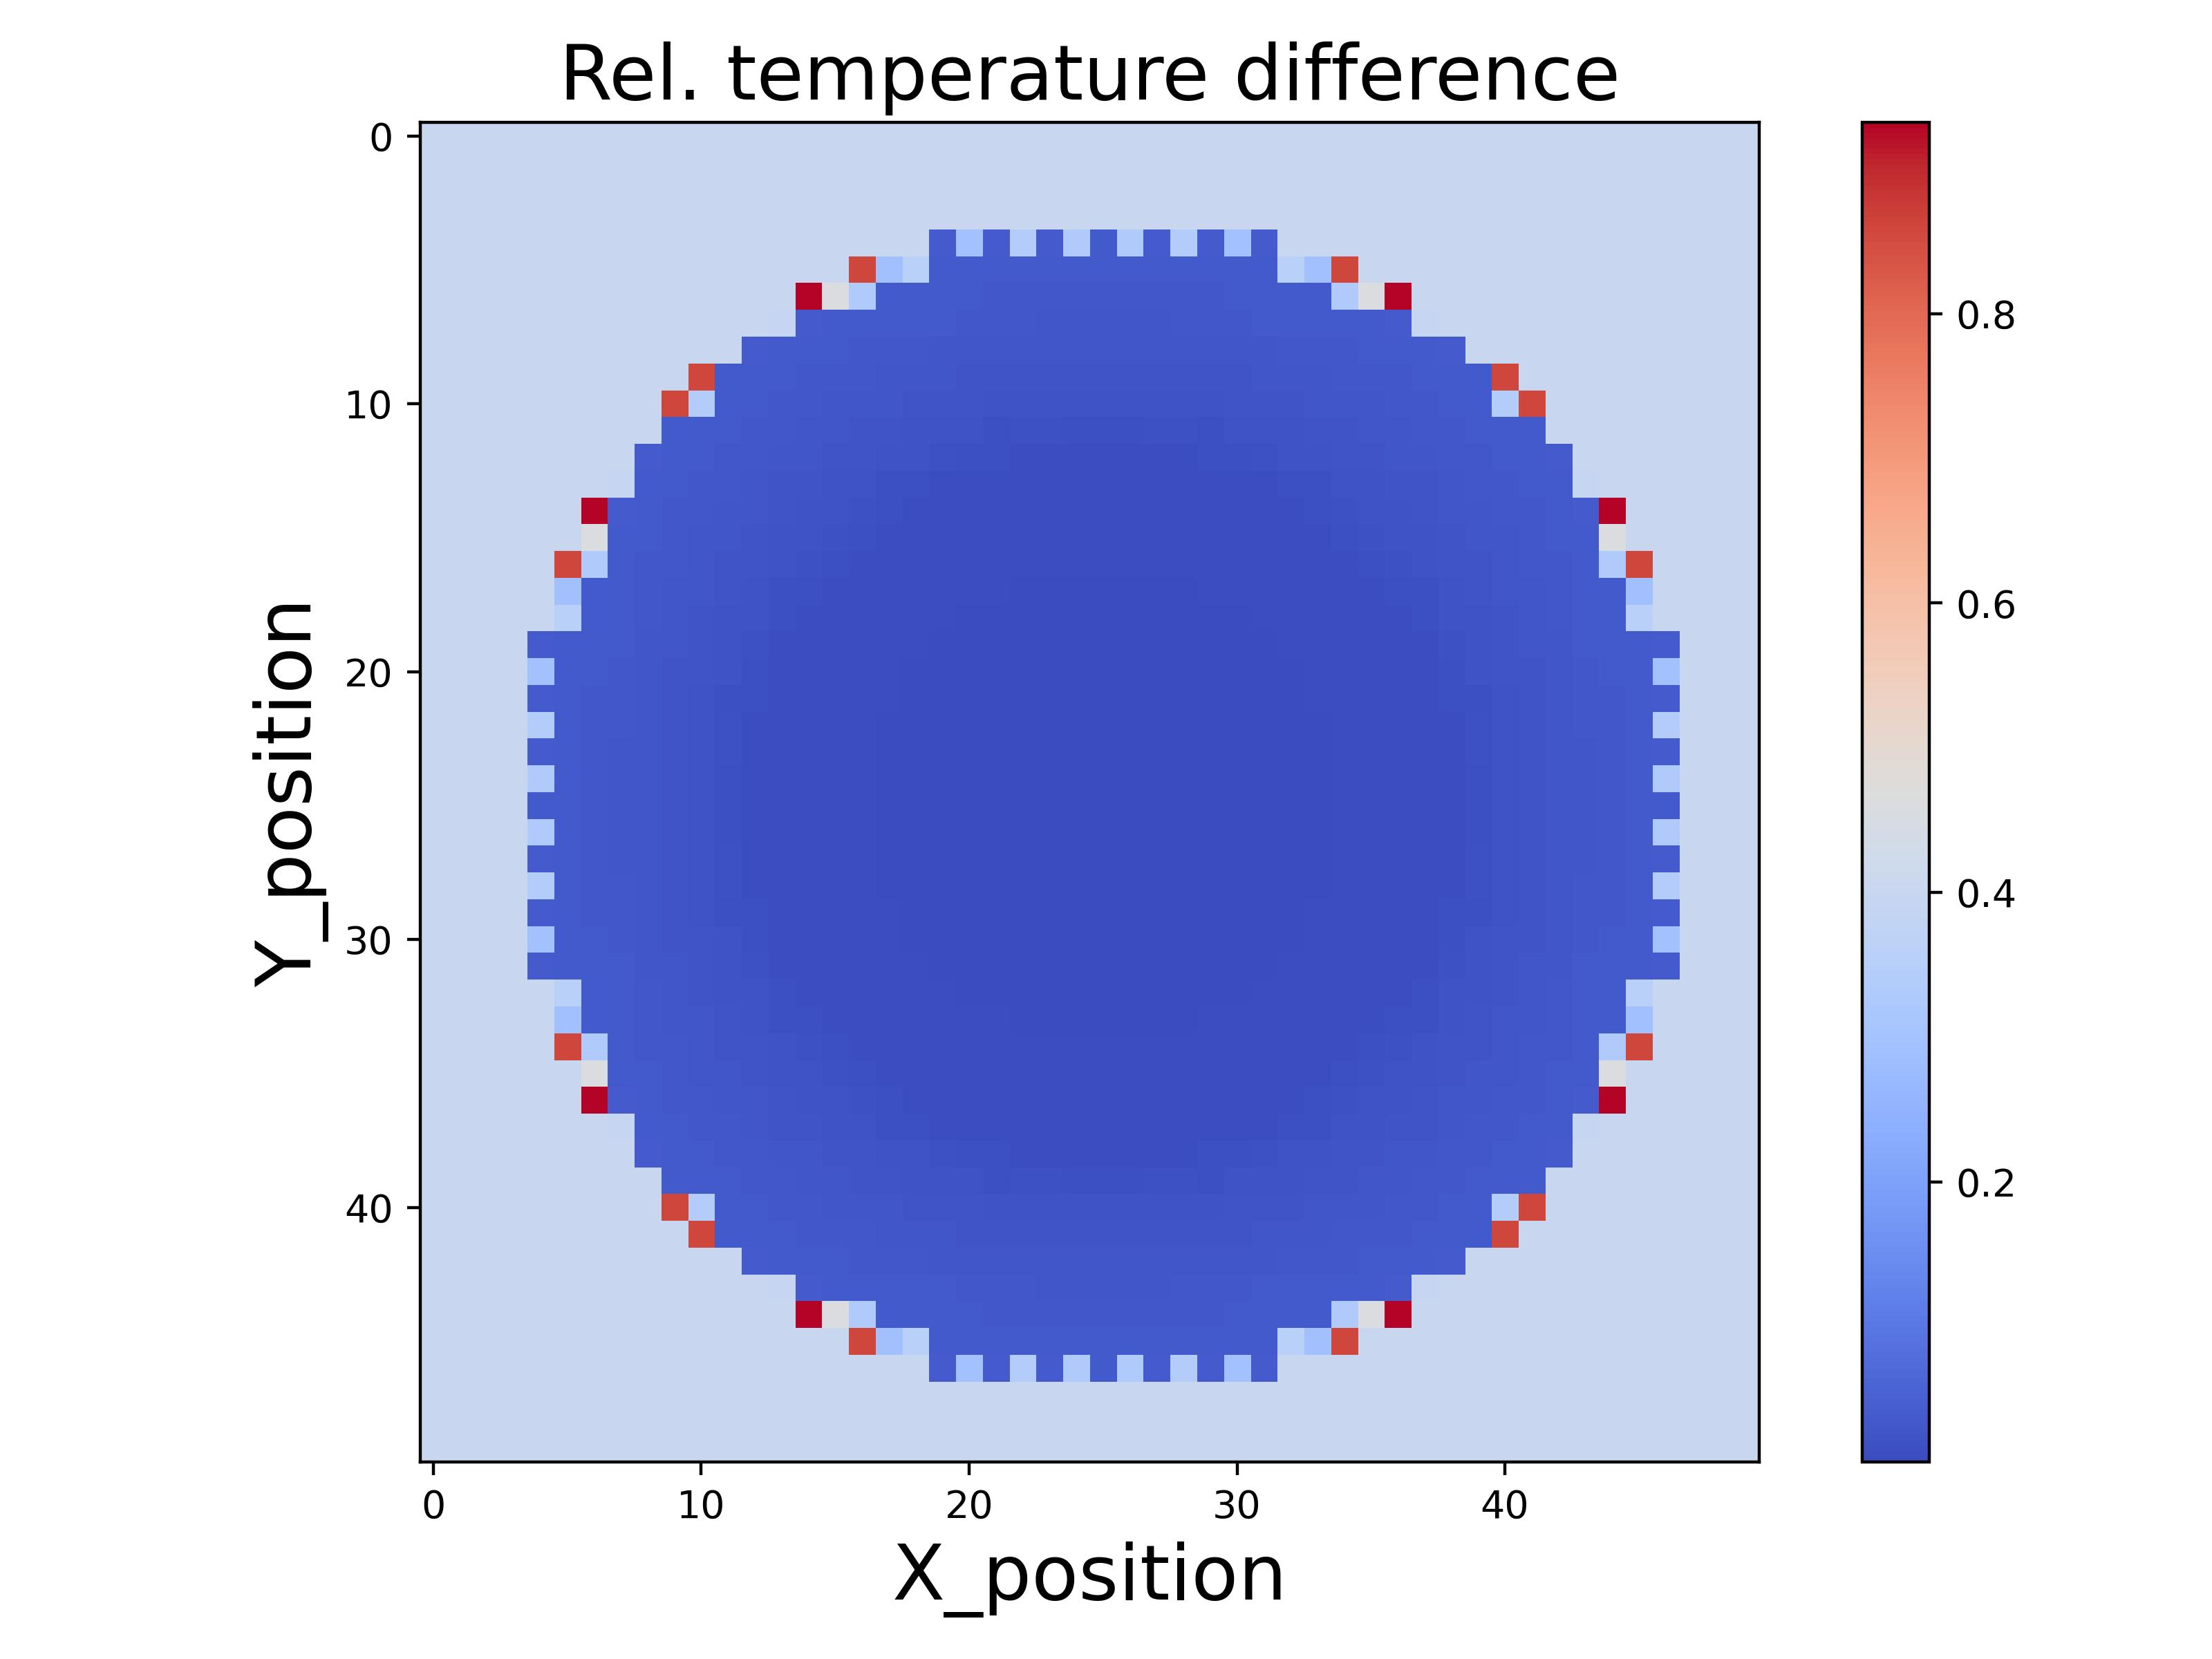
\includegraphics[width=\textwidth]{figures/raw_data/0/linear/T_bias.jpg}
            \subcaption{Black body material}
        \end{subfigure}
        \begin{subfigure}{0.28\textwidth}
            \centering
            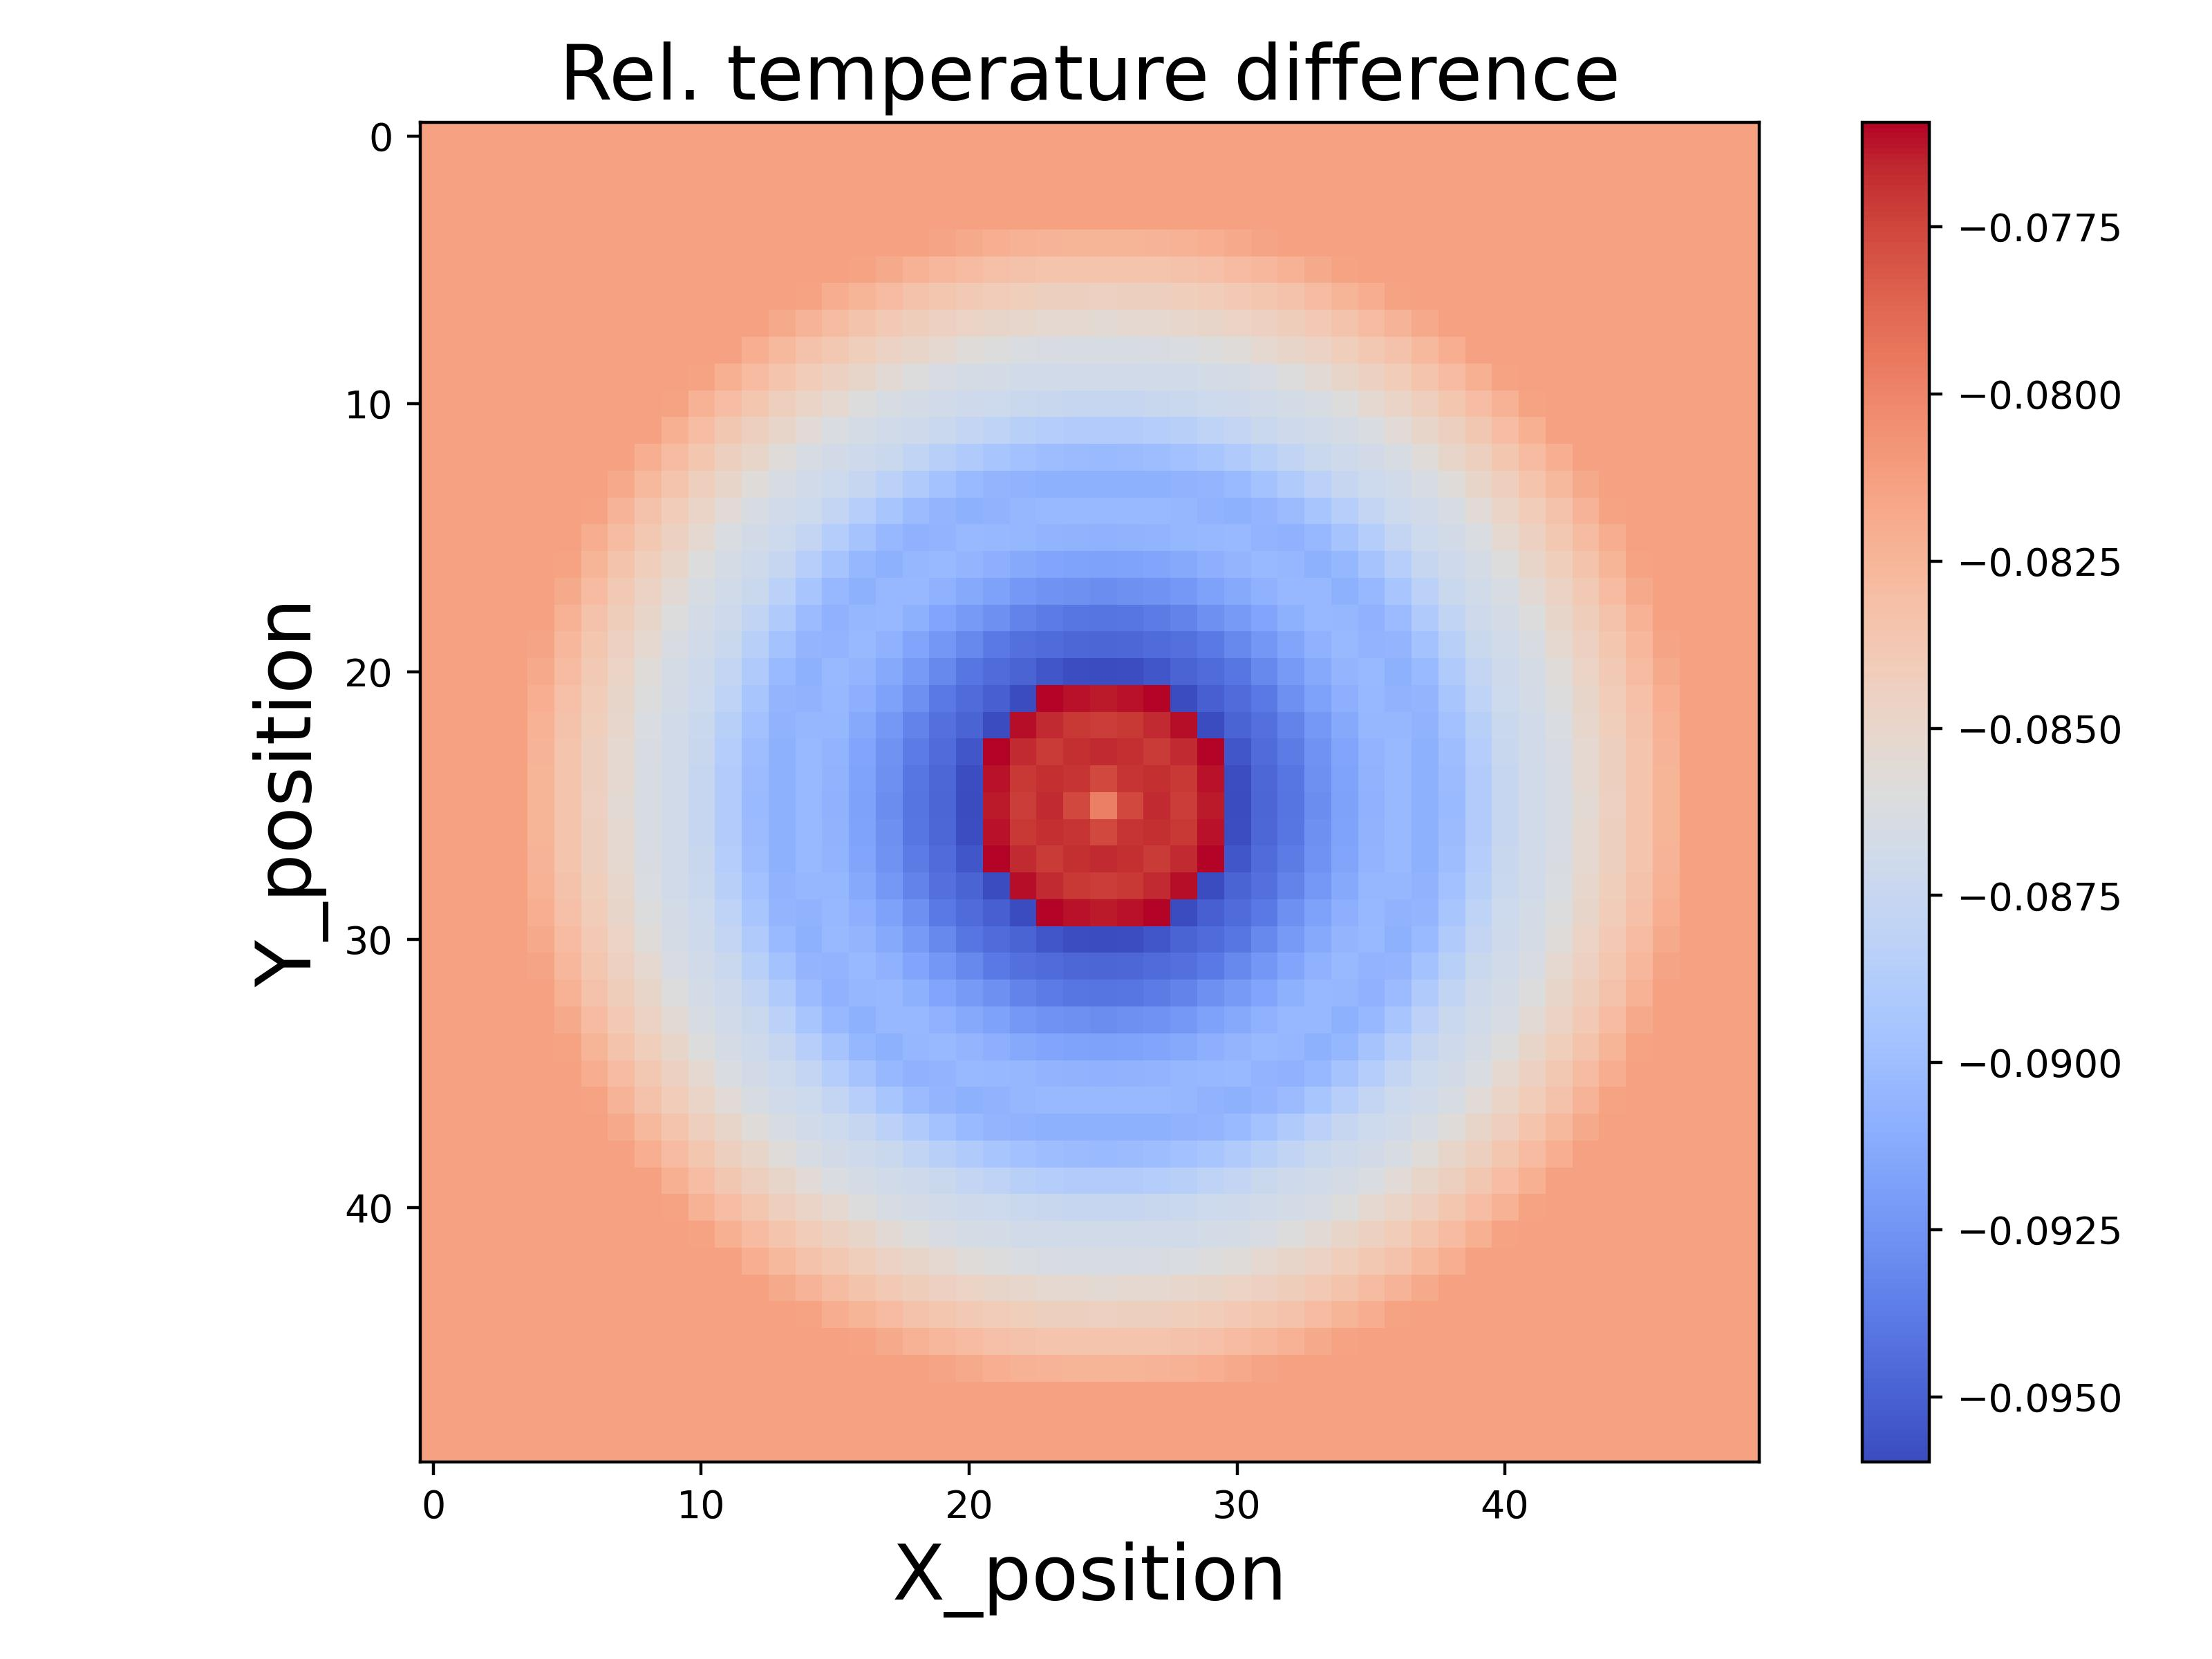
\includegraphics[width=\textwidth]{figures/raw_data/5/linear/T_bias.jpg}
            \subcaption{Real iron data}
        \end{subfigure}
        \begin{subfigure}{0.28\textwidth}
            \centering
            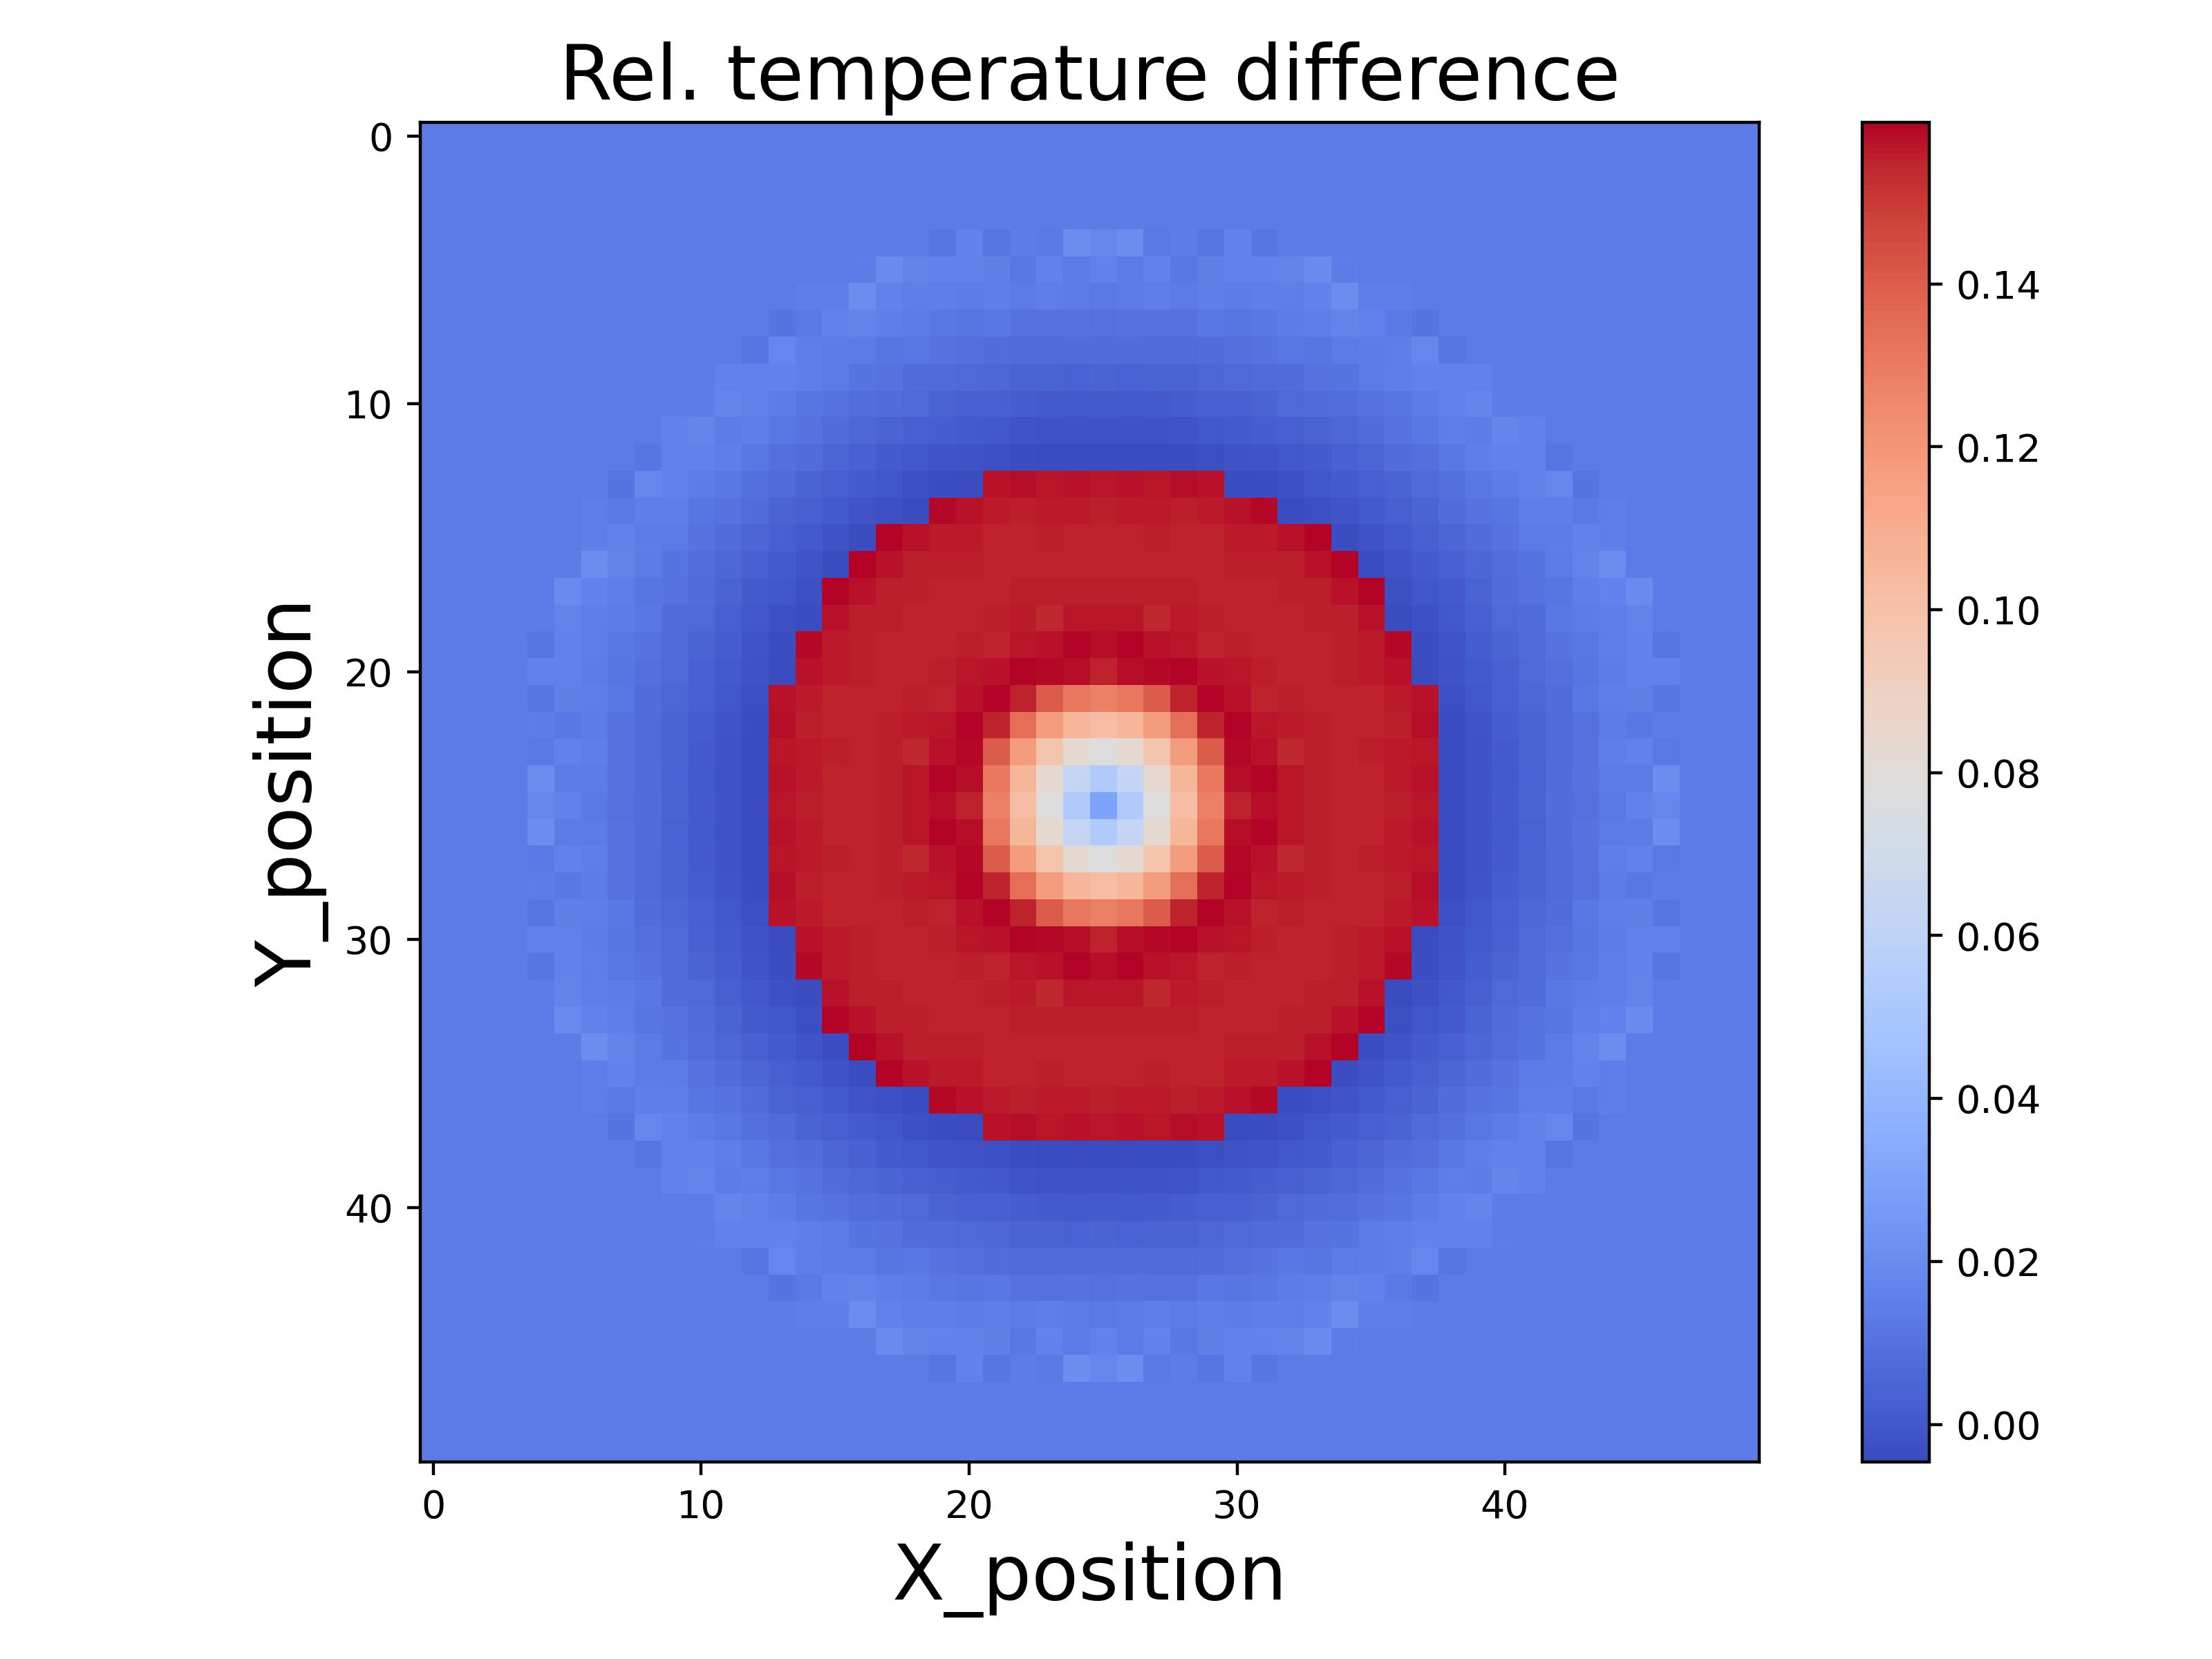
\includegraphics[width=\textwidth]{figures/raw_data/21/linear/T_bias.jpg}
            \subcaption{Model 1}
        \end{subfigure}
    \end{minipage}\\
    \begin{minipage}{\textwidth}
        \centering
        \begin{subfigure}{0.28\textwidth}
            \centering
            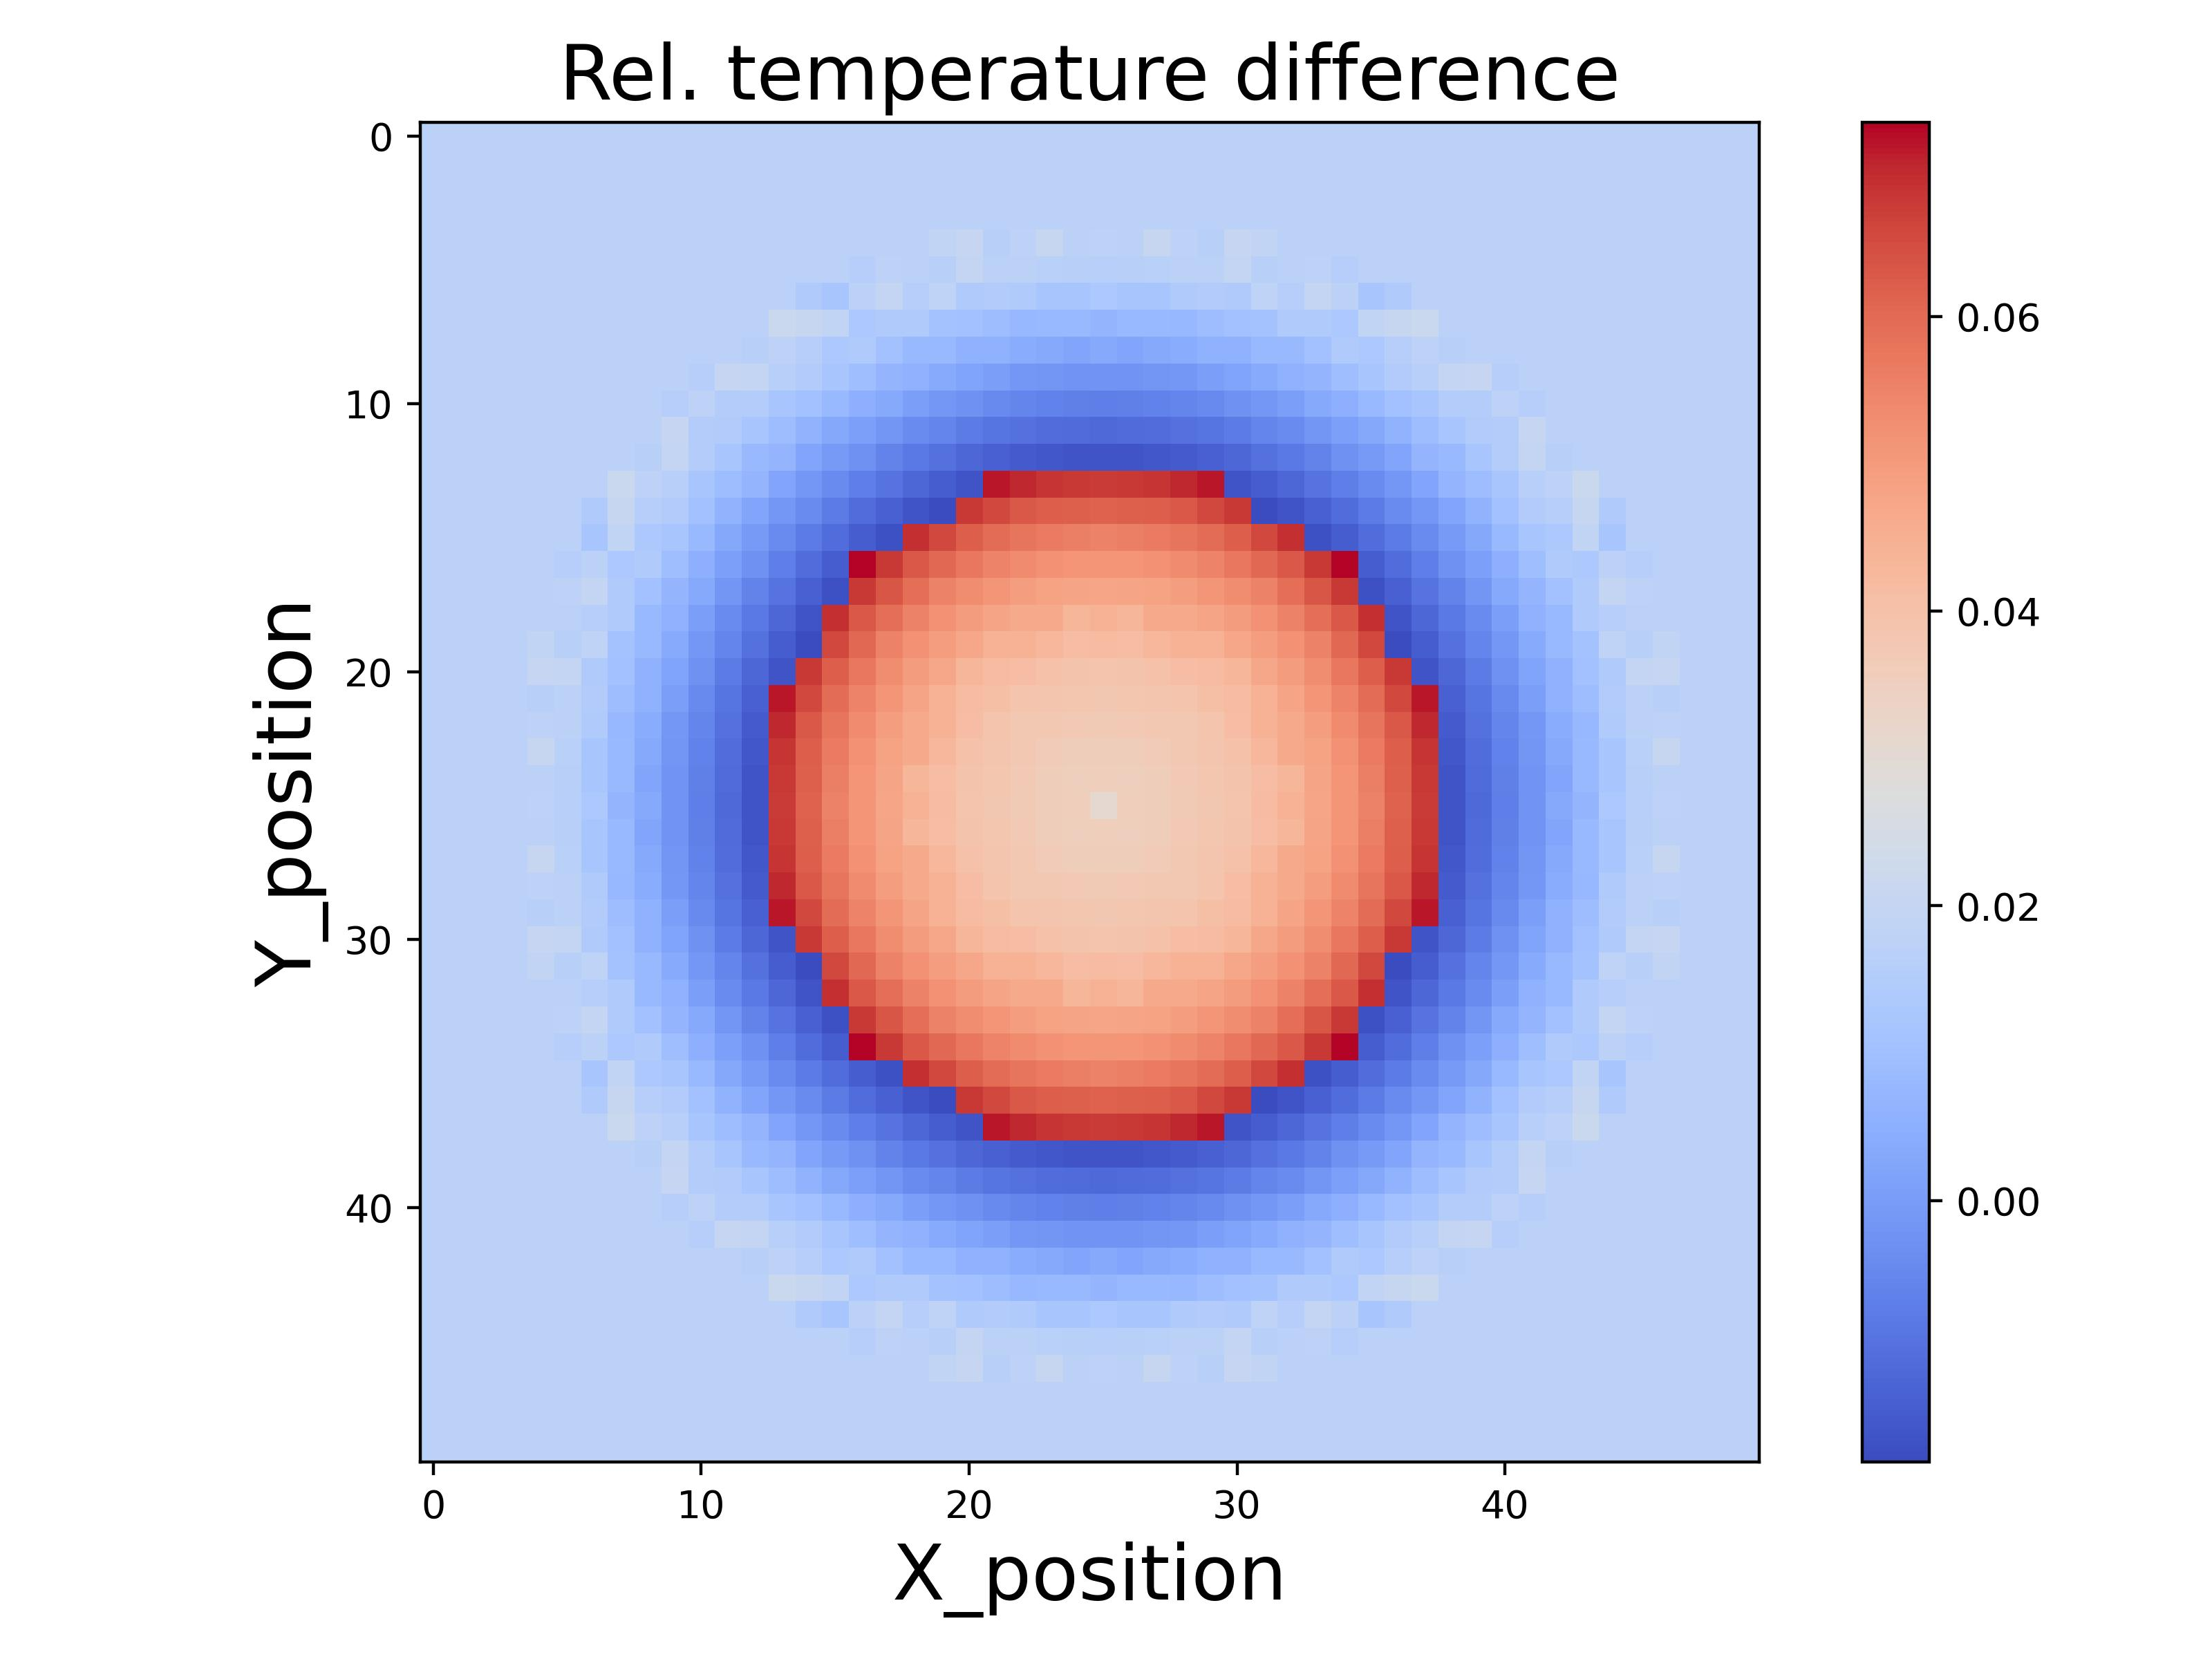
\includegraphics[width=\textwidth]{figures/raw_data/22/linear/T_bias.jpg}
            \subcaption{Model 2}
        \end{subfigure}
        \begin{subfigure}{0.28\textwidth}
            \centering
            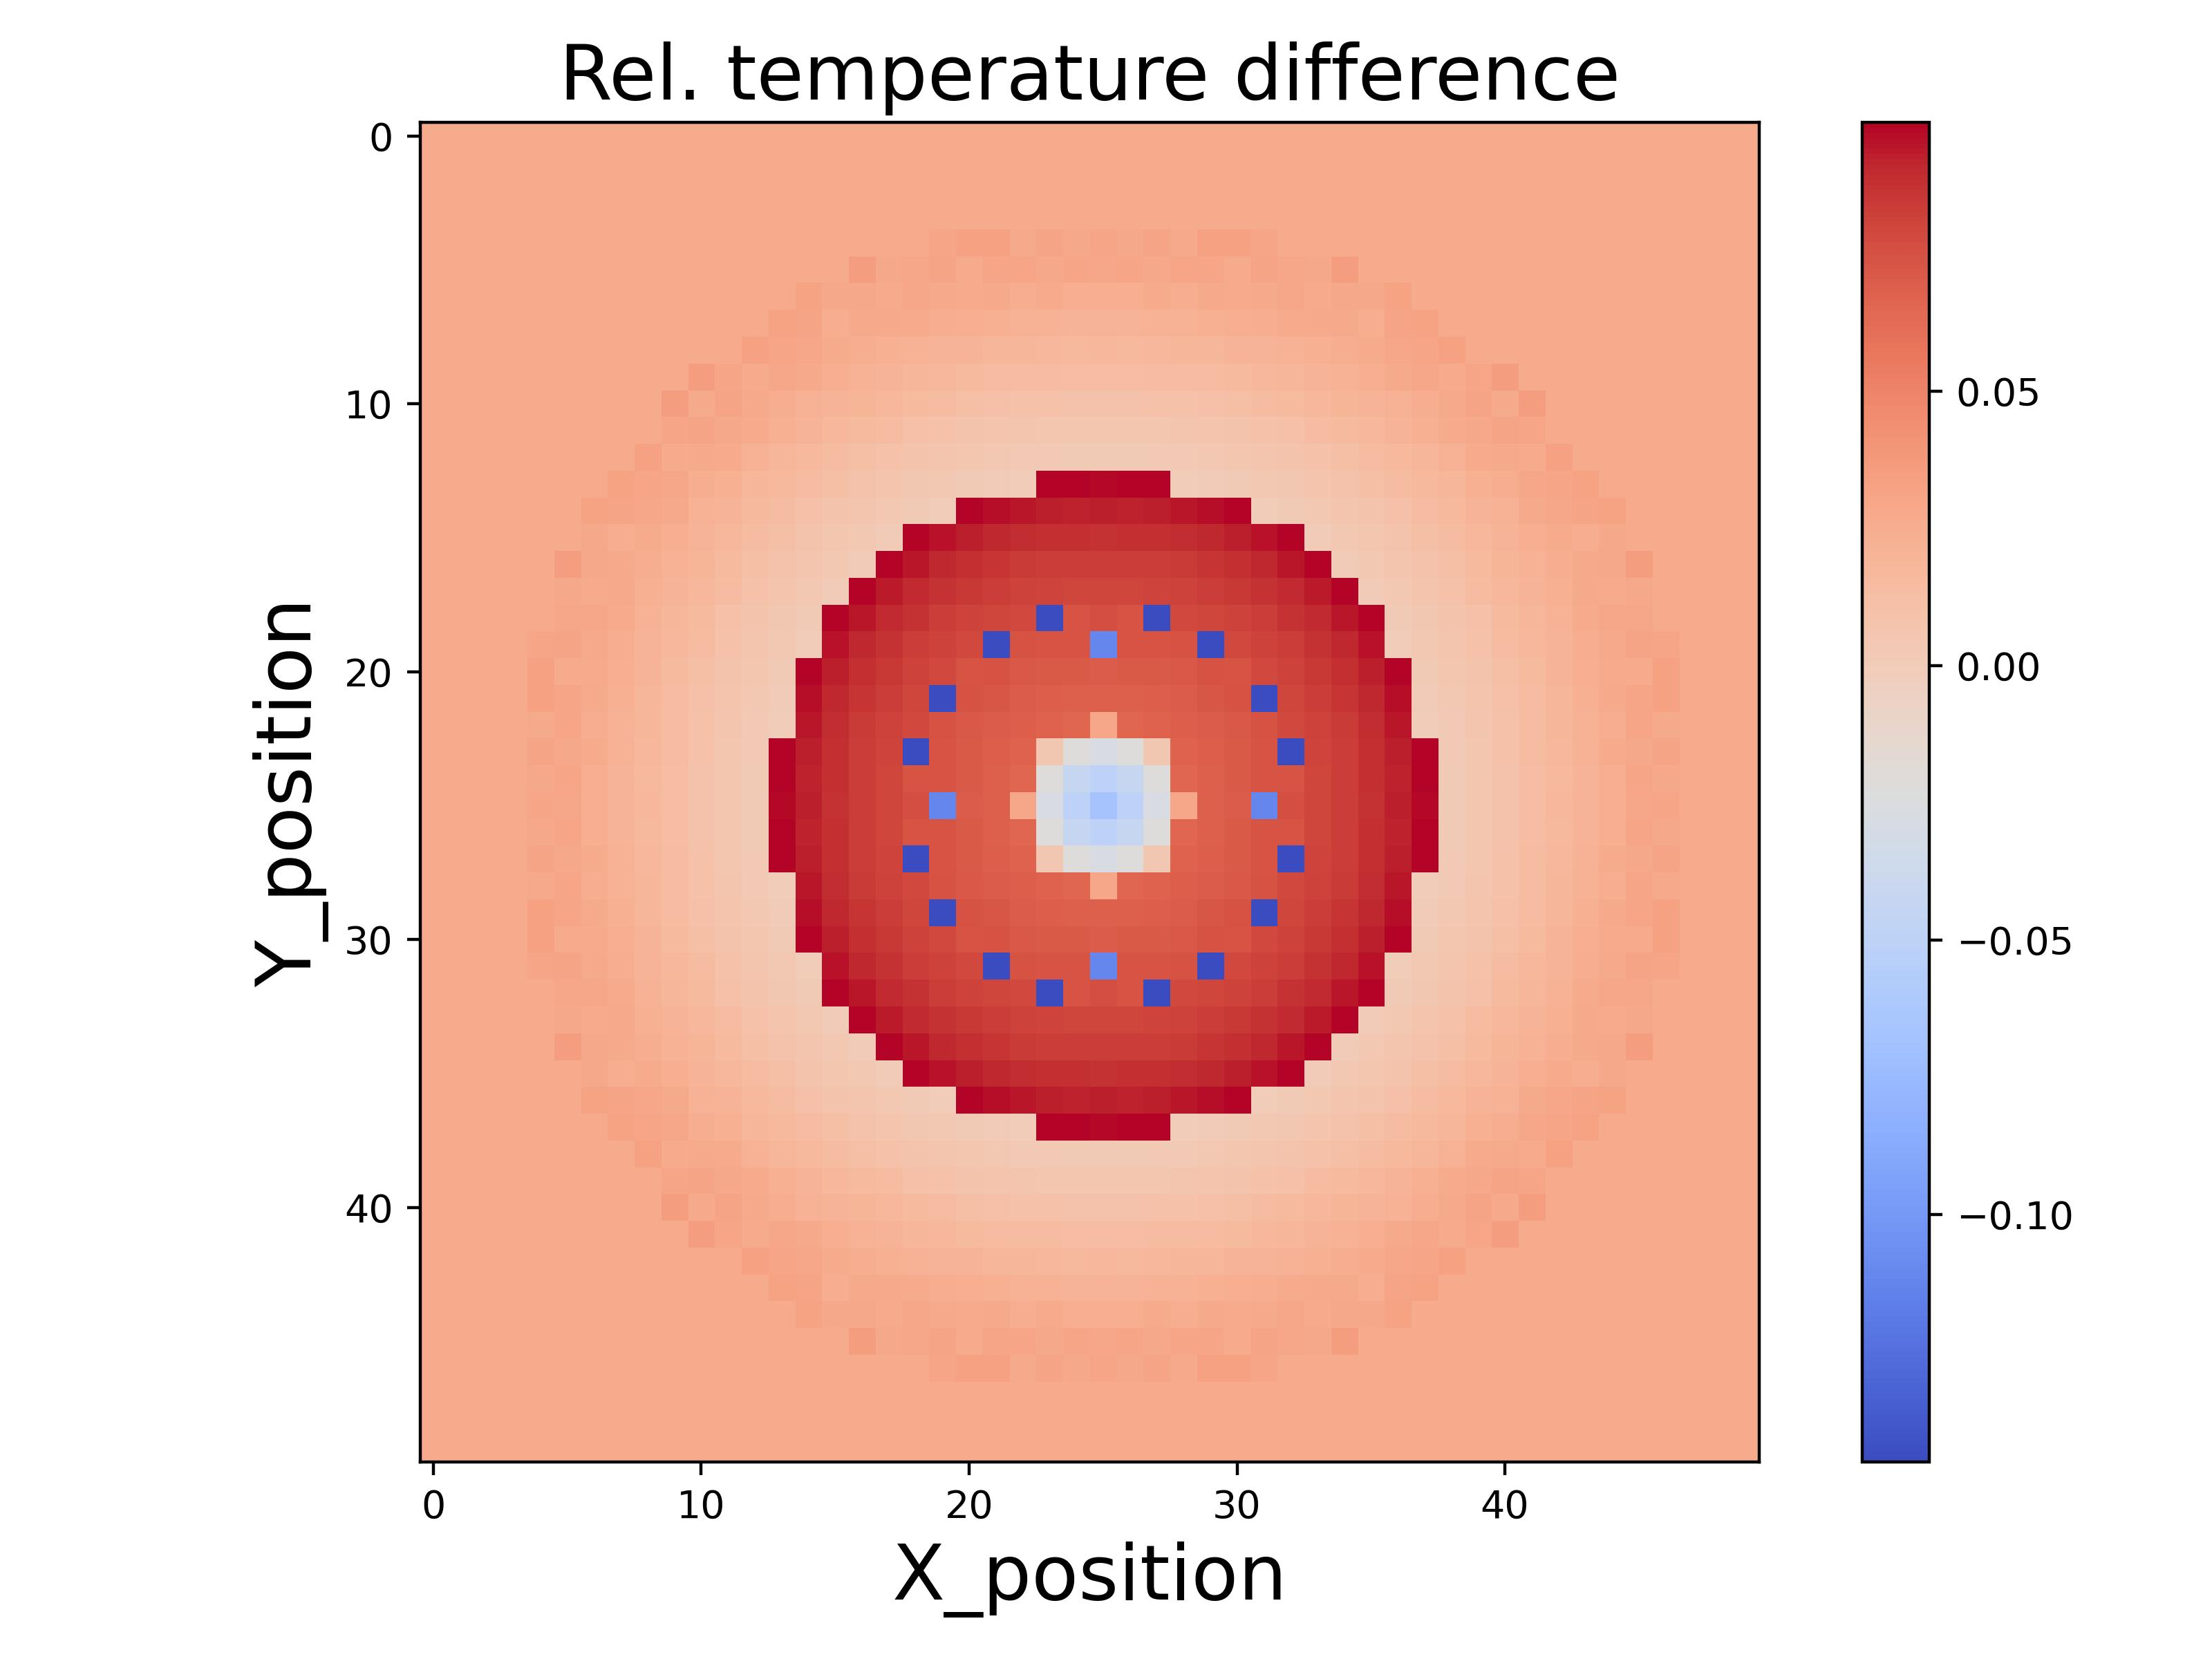
\includegraphics[width=\textwidth]{figures/raw_data/23/linear/T_bias.jpg}
            \subcaption{Model 3}
        \end{subfigure}
        \begin{subfigure}{0.28\textwidth}
            \centering
            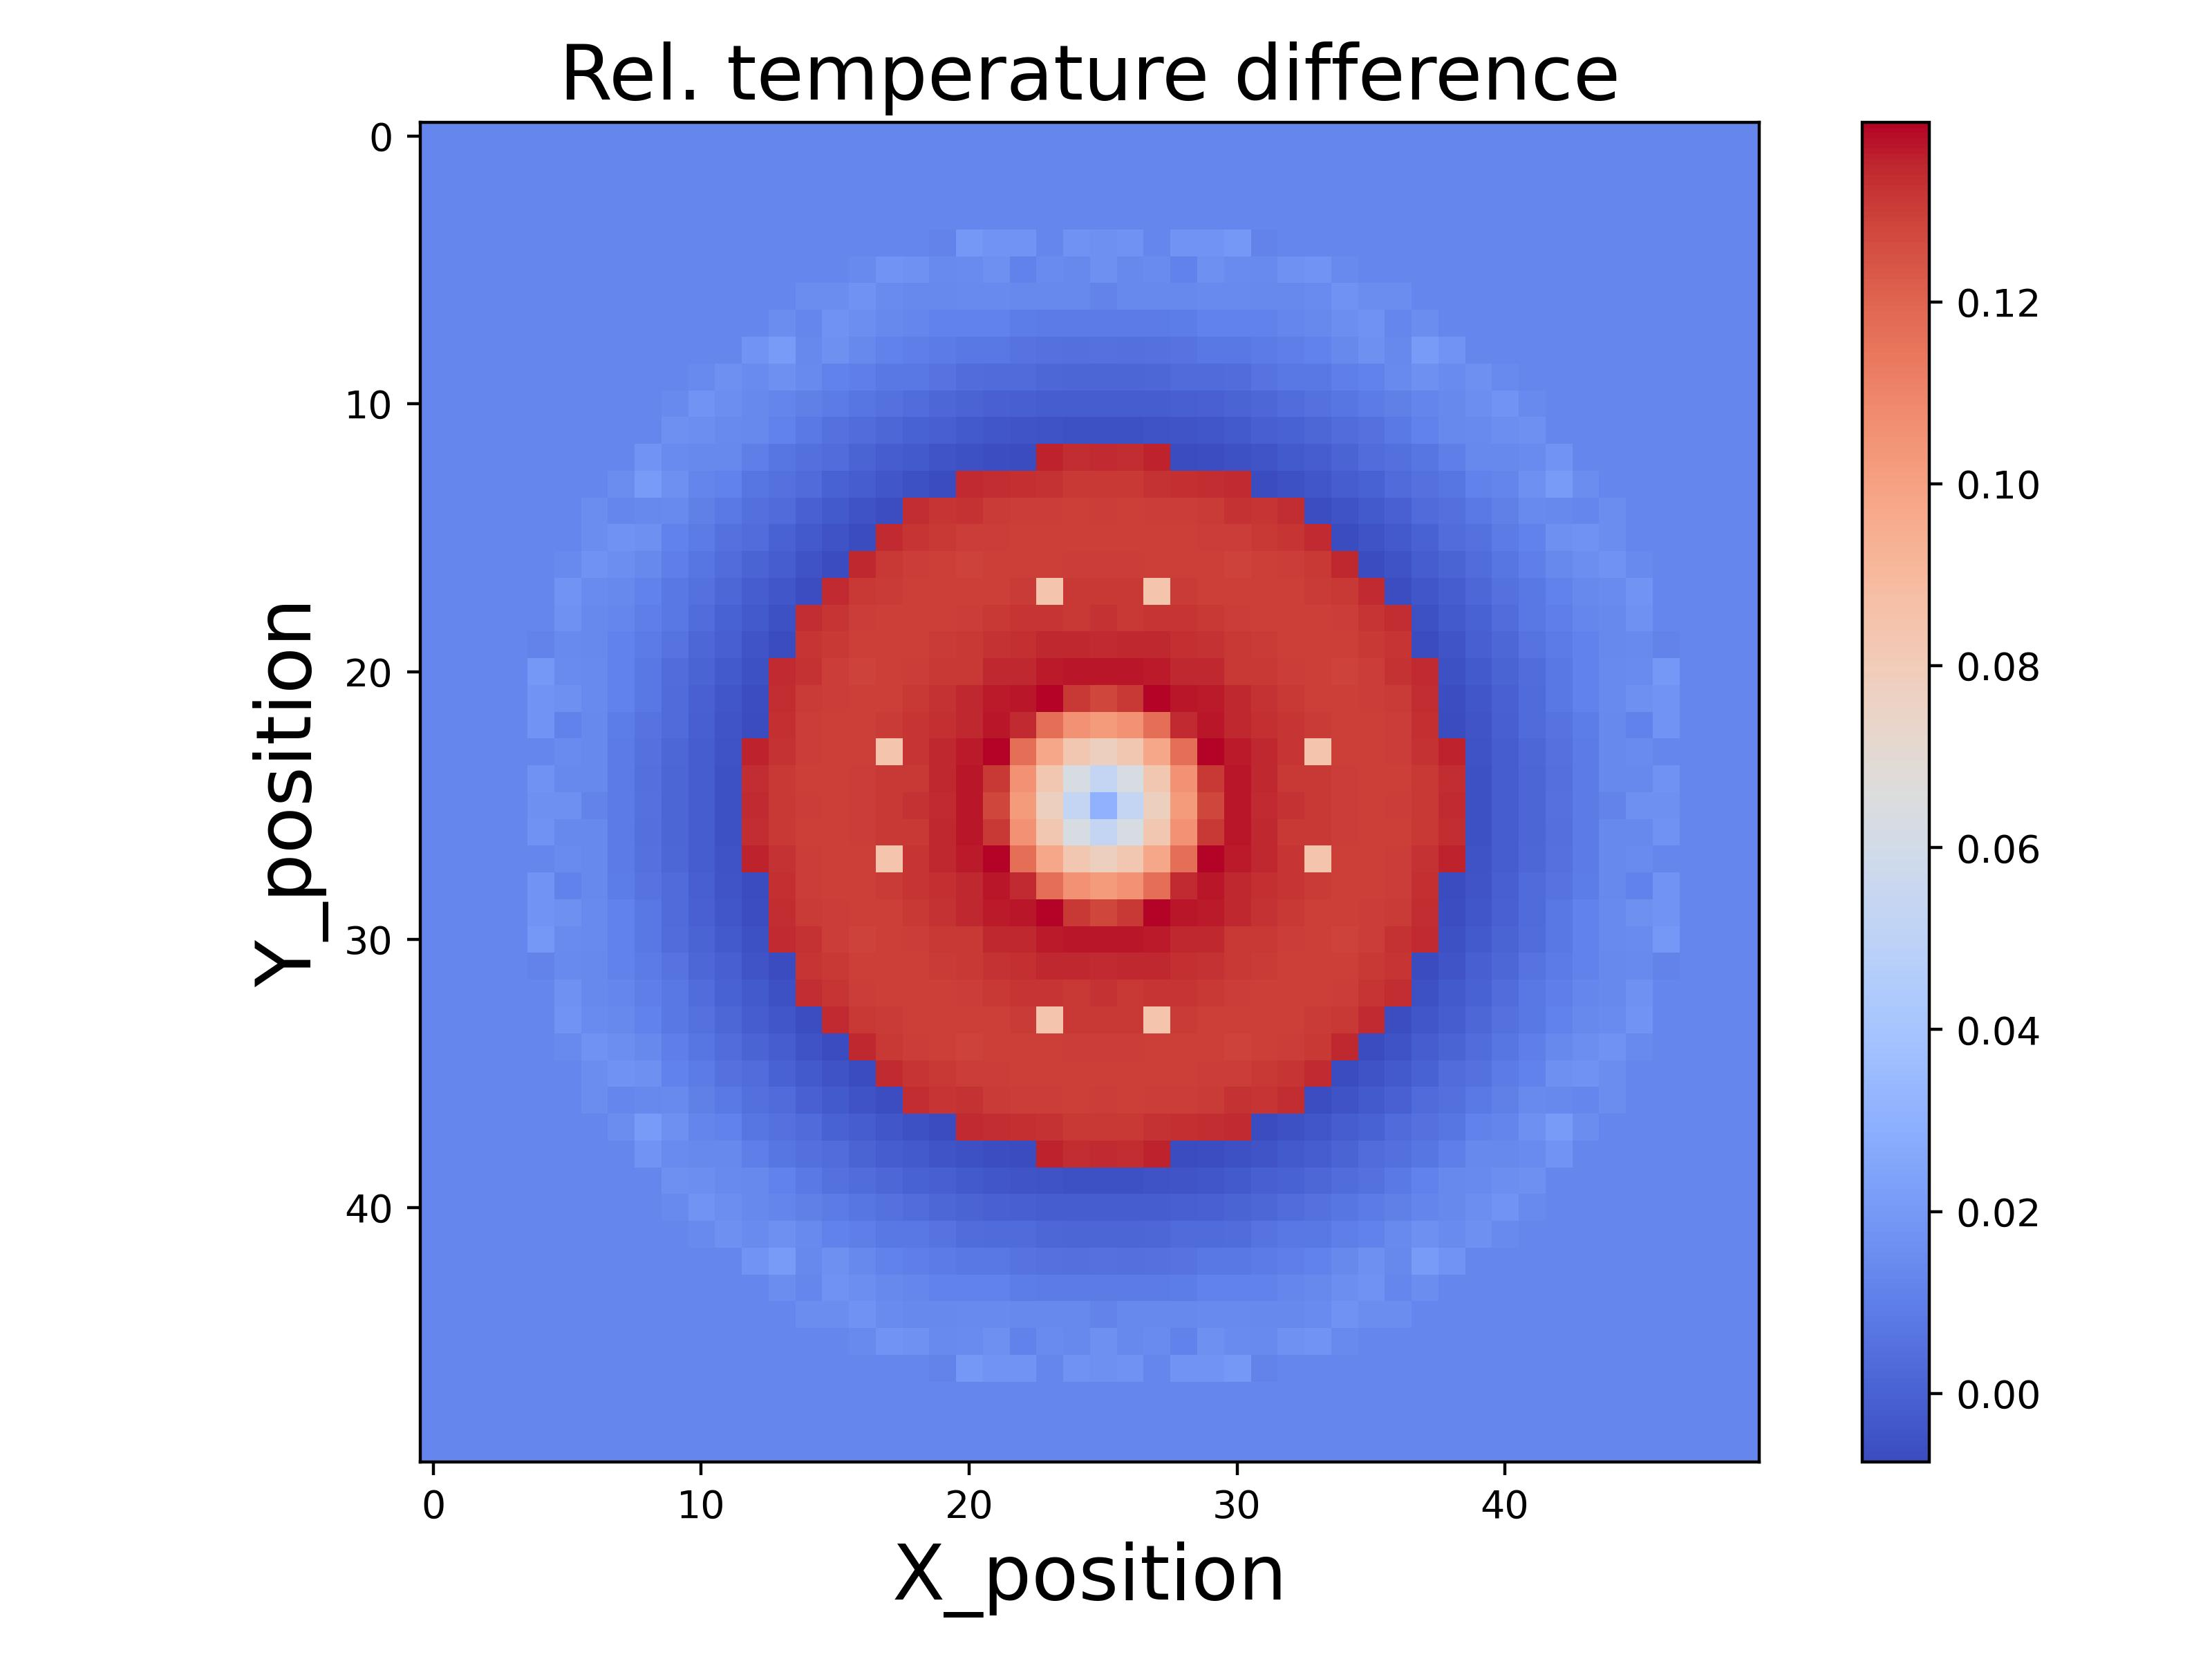
\includegraphics[width=\textwidth]{figures/raw_data/24/linear/T_bias.jpg}
            \subcaption{Model 4}
        \end{subfigure}
    \end{minipage}\\
    \begin{minipage}{\textwidth}
        \centering
        \begin{subfigure}{0.28\textwidth}
            \centering
            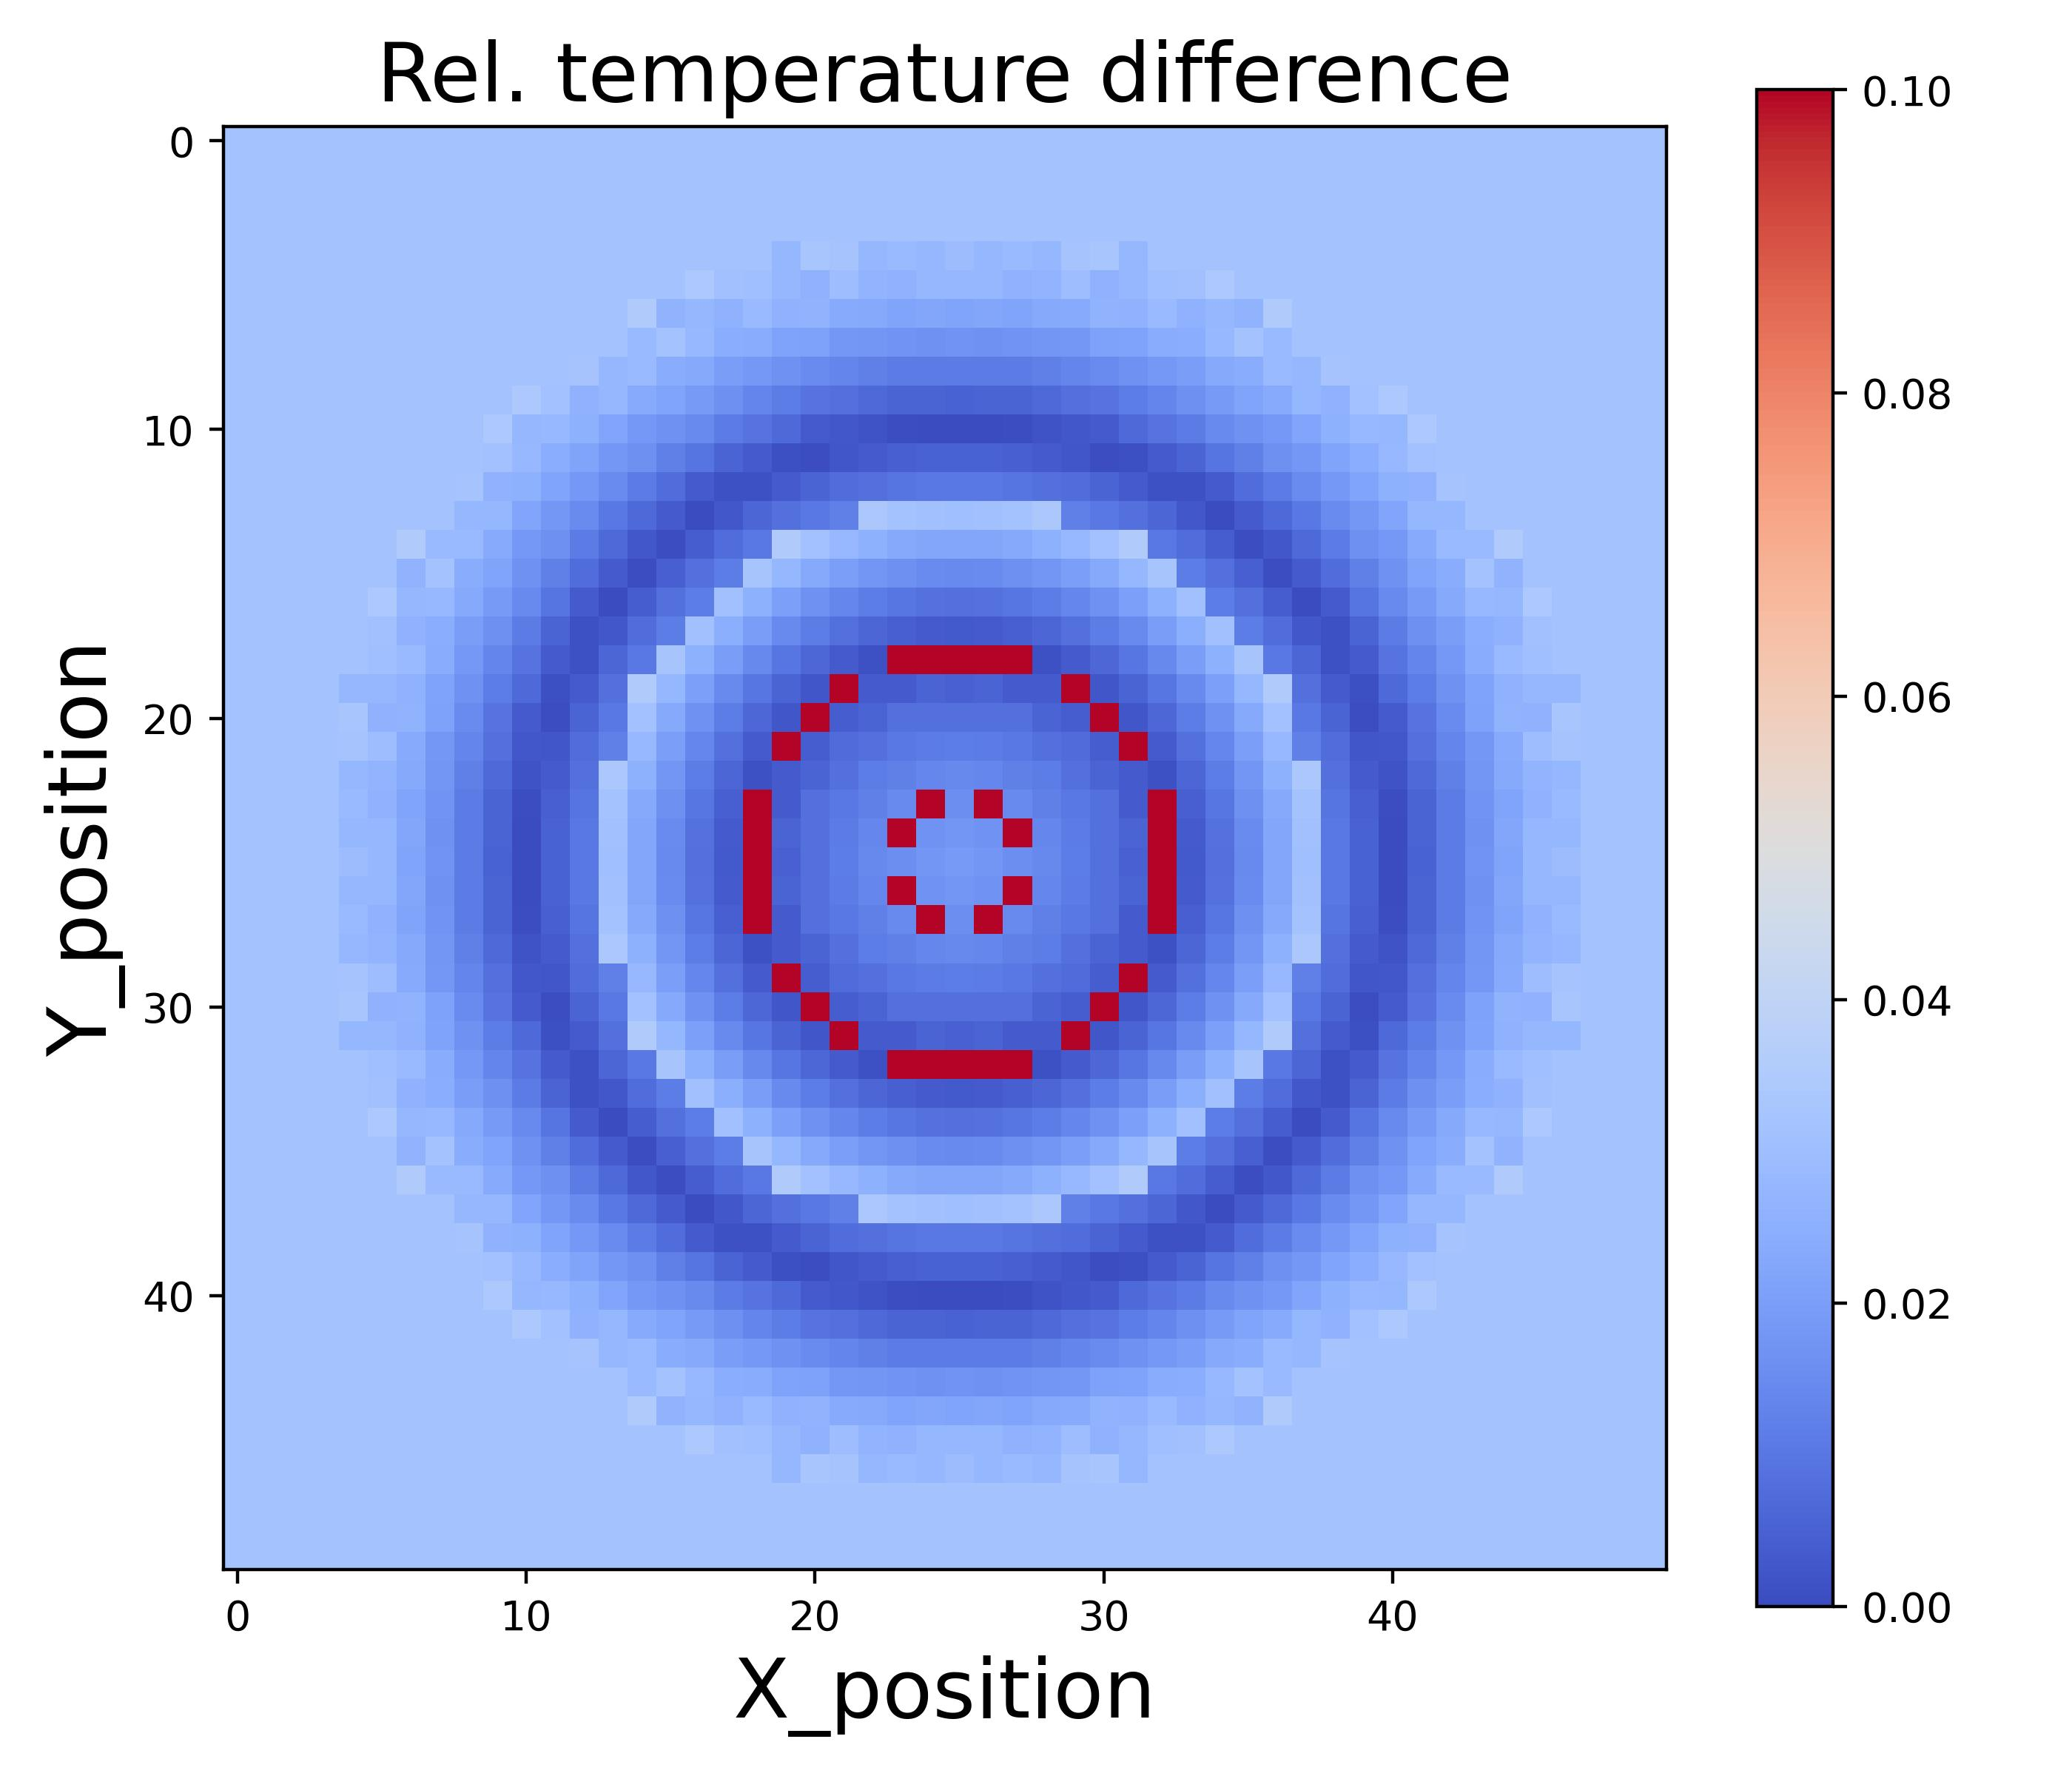
\includegraphics[width=\textwidth]{figures/raw_data/25/linear/T_bias.jpg}
            \subcaption{Model 5}
        \end{subfigure}
        \begin{subfigure}{0.28\textwidth}
            \centering
            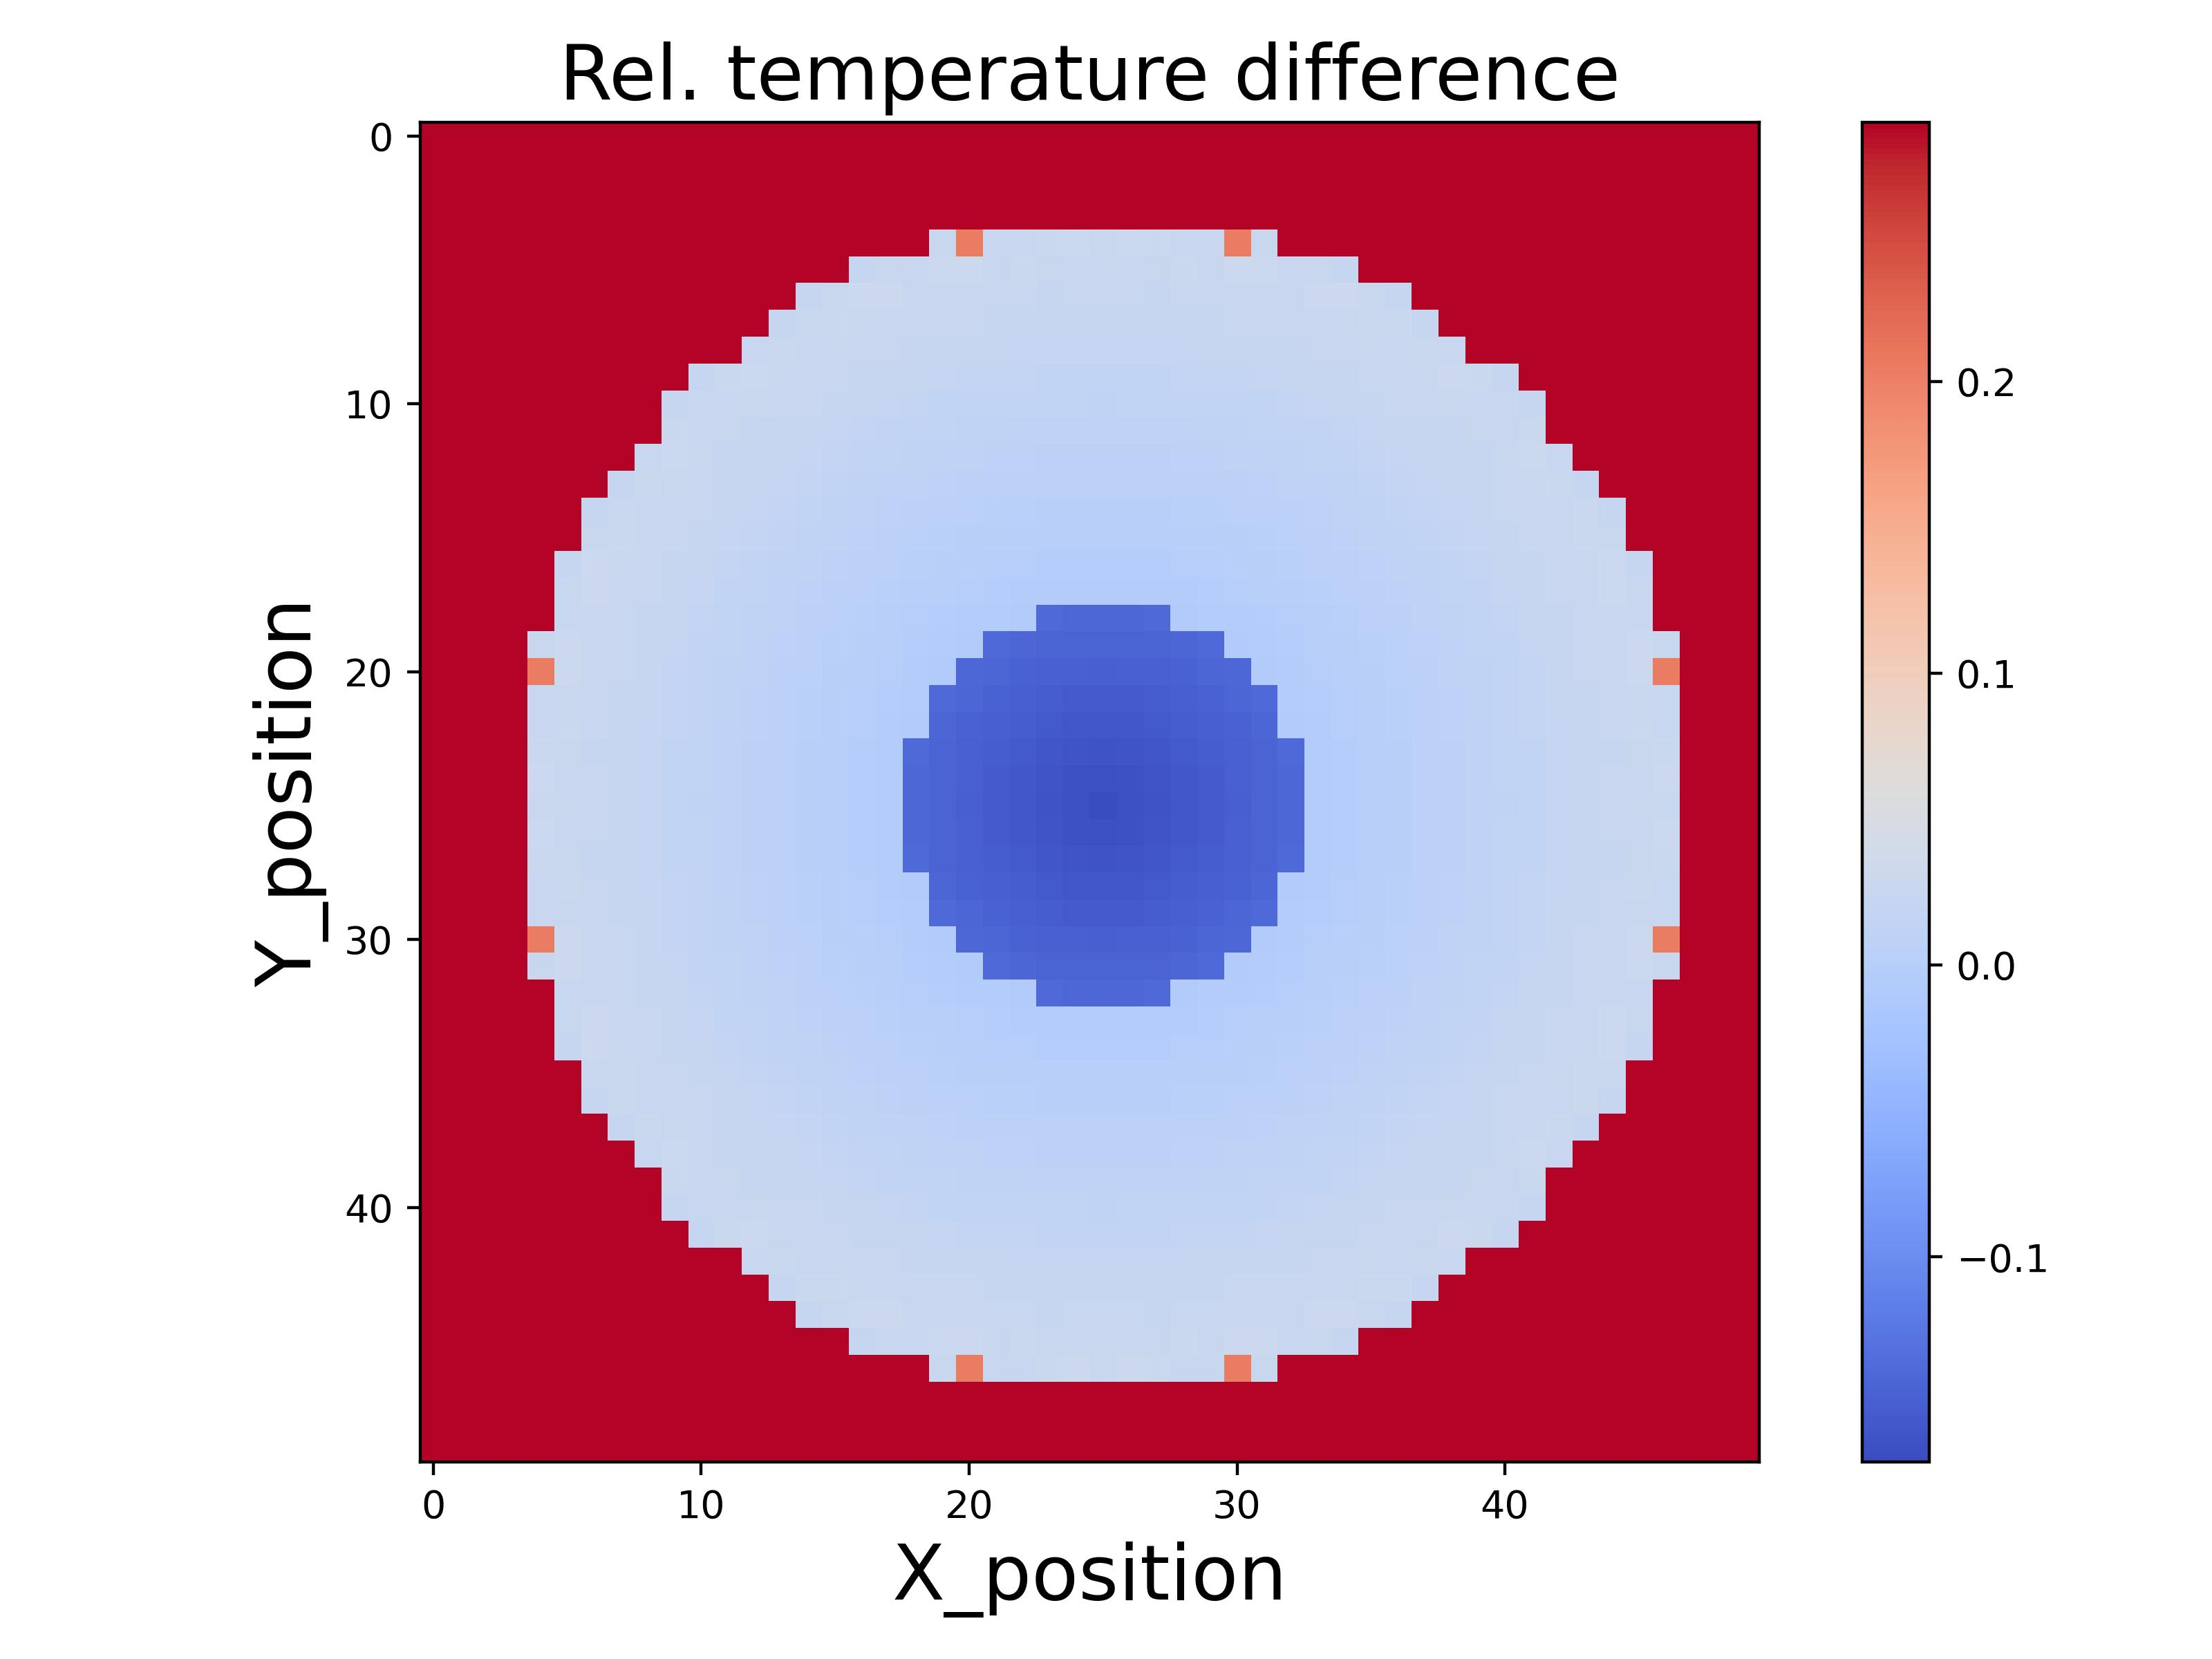
\includegraphics[width=\textwidth]{figures/raw_data/26/linear/T_bias.jpg}
            \subcaption{Model 6}
        \end{subfigure}
        \begin{subfigure}{0.28\textwidth}
            \centering
            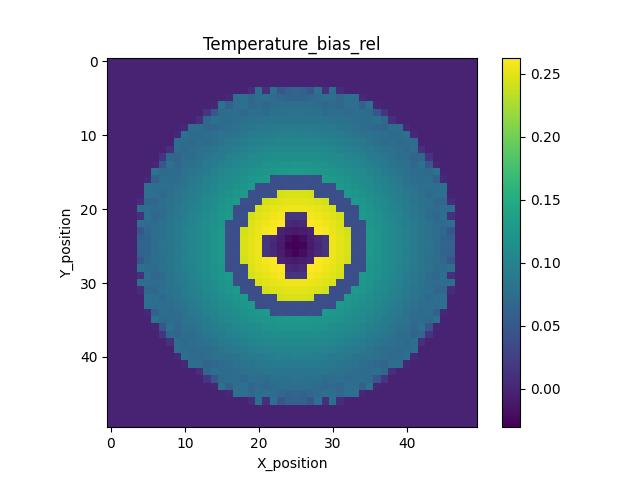
\includegraphics[width=\textwidth]{figures/raw_data/31/linear/T_bias.jpg}
            \subcaption{Model 7}
        \end{subfigure}
    \end{minipage}\\
    \begin{minipage}{\textwidth}
        \centering
        \begin{subfigure}{0.28\textwidth}
            \centering
            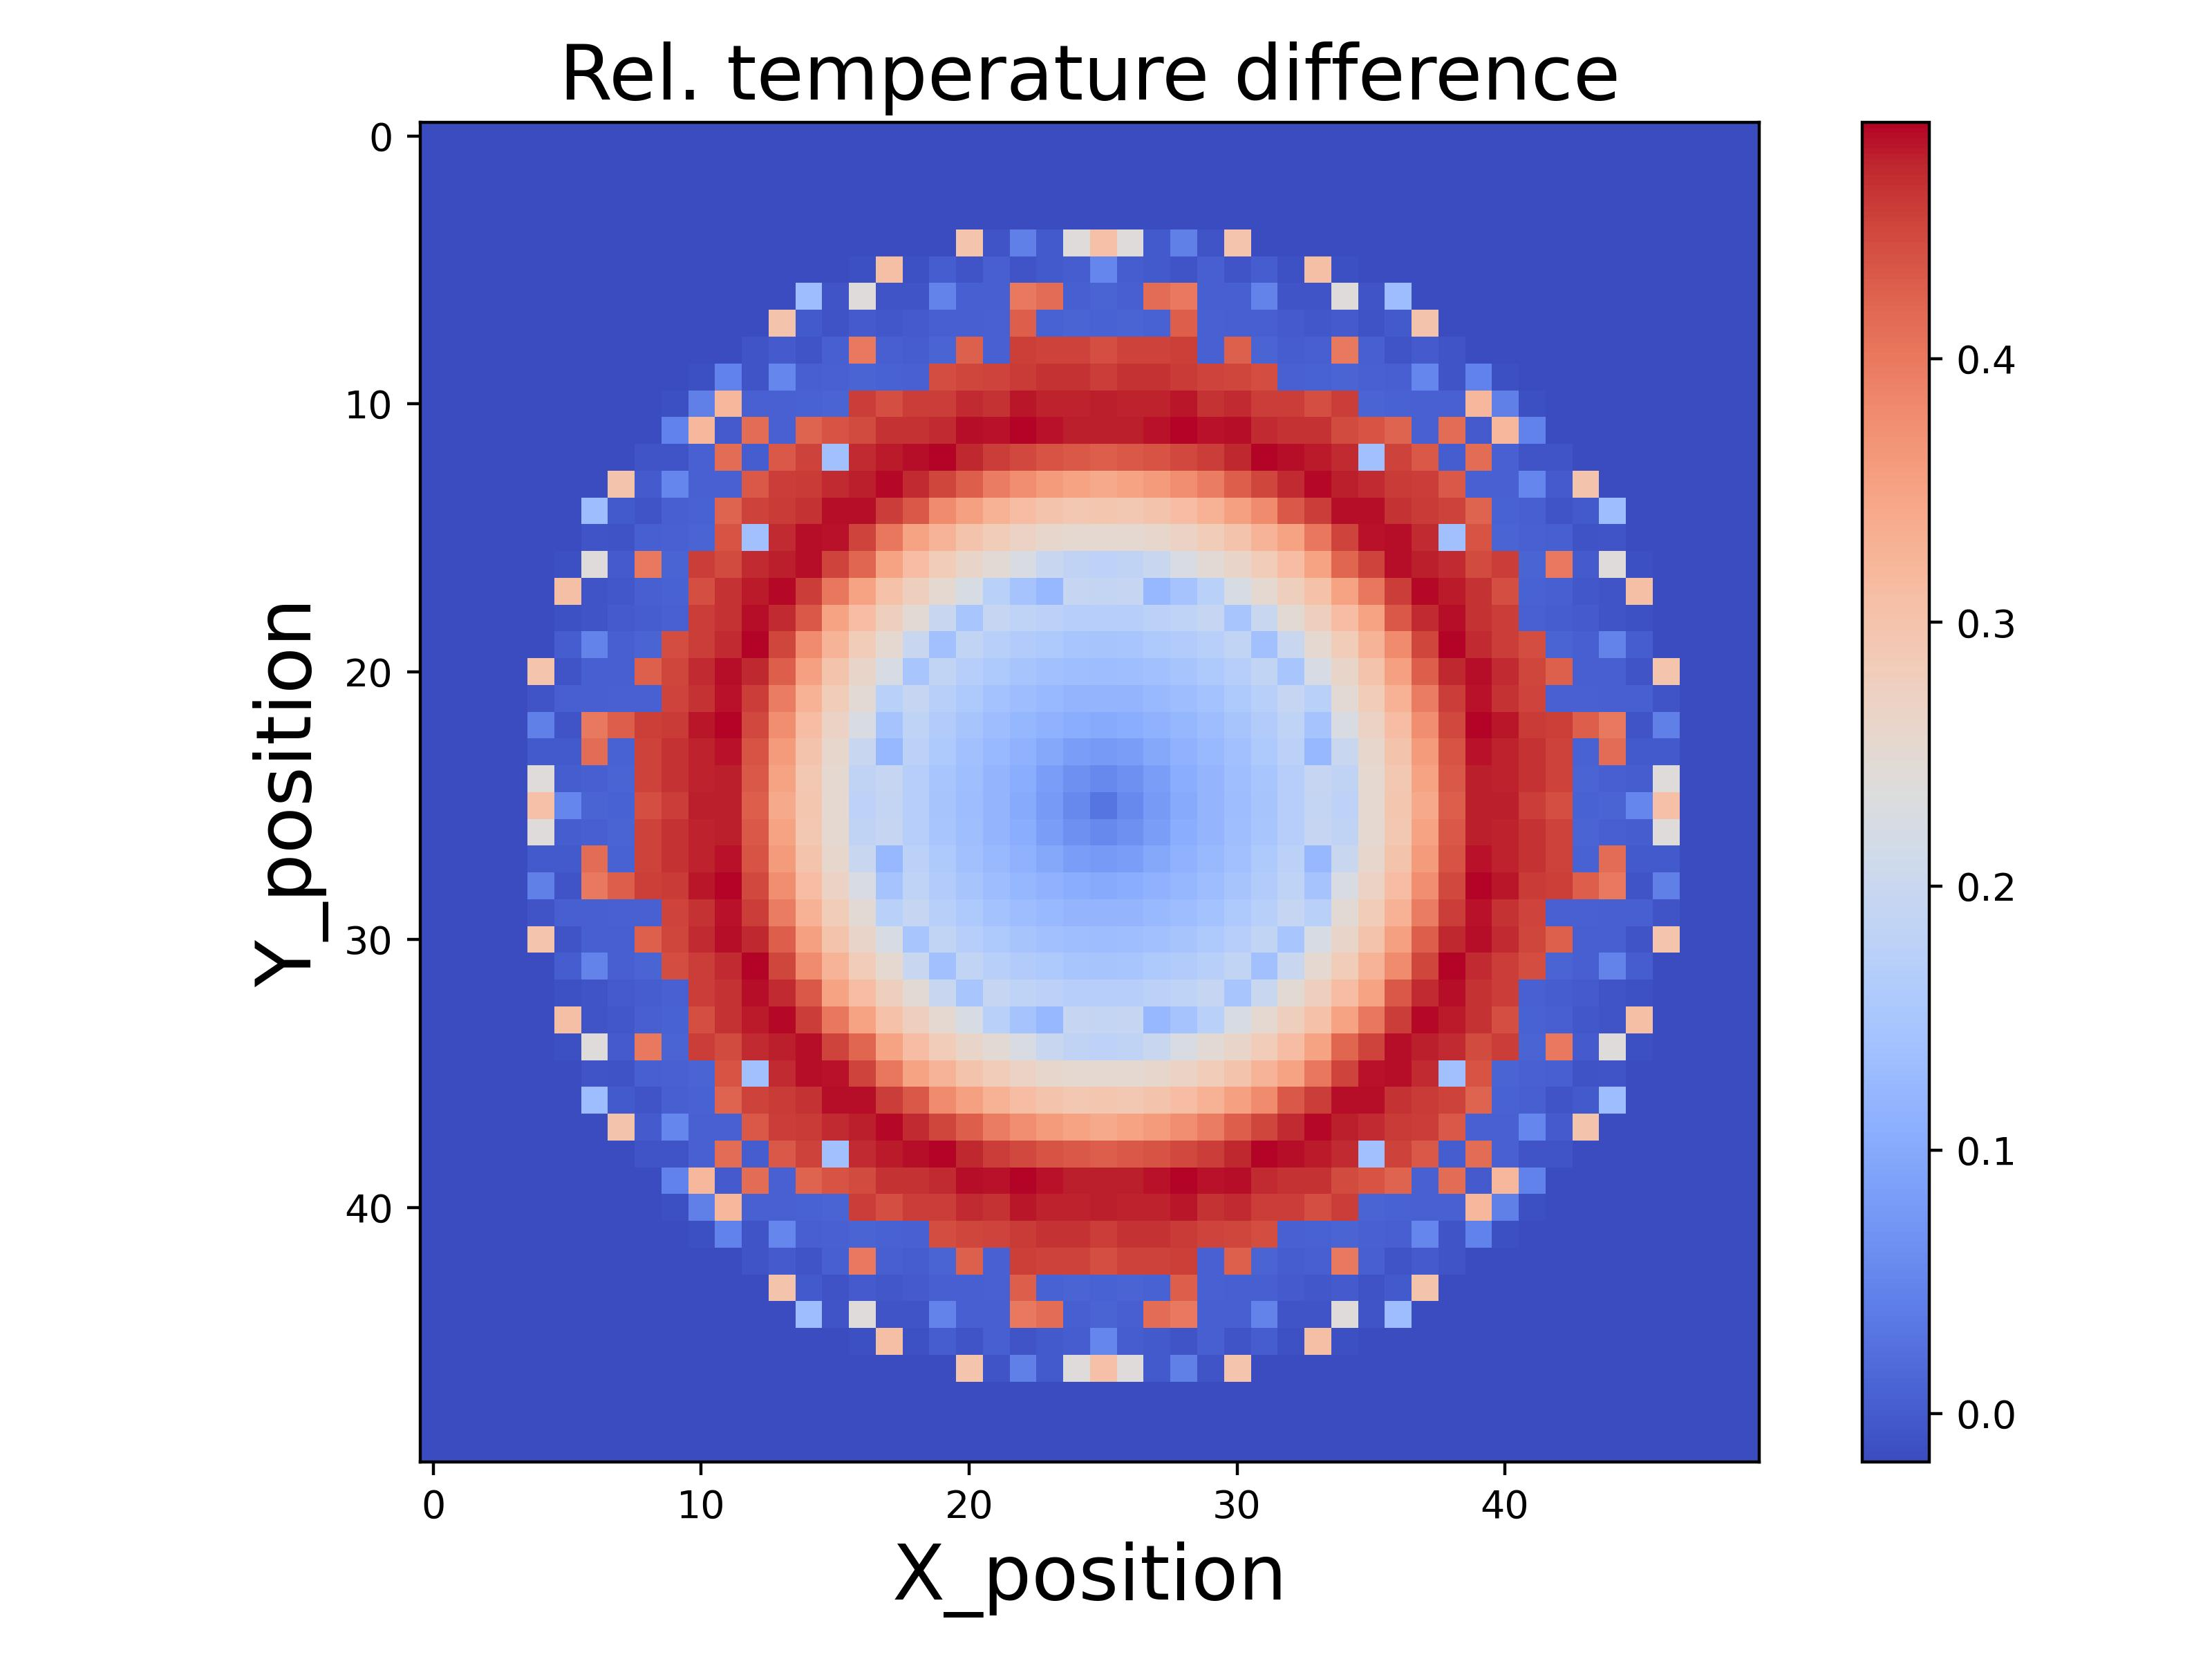
\includegraphics[width=\textwidth]{figures/raw_data/32/linear/T_bias.jpg}
            \subcaption{Model 8}
        \end{subfigure}
        \begin{subfigure}{0.28\textwidth}
            \centering
            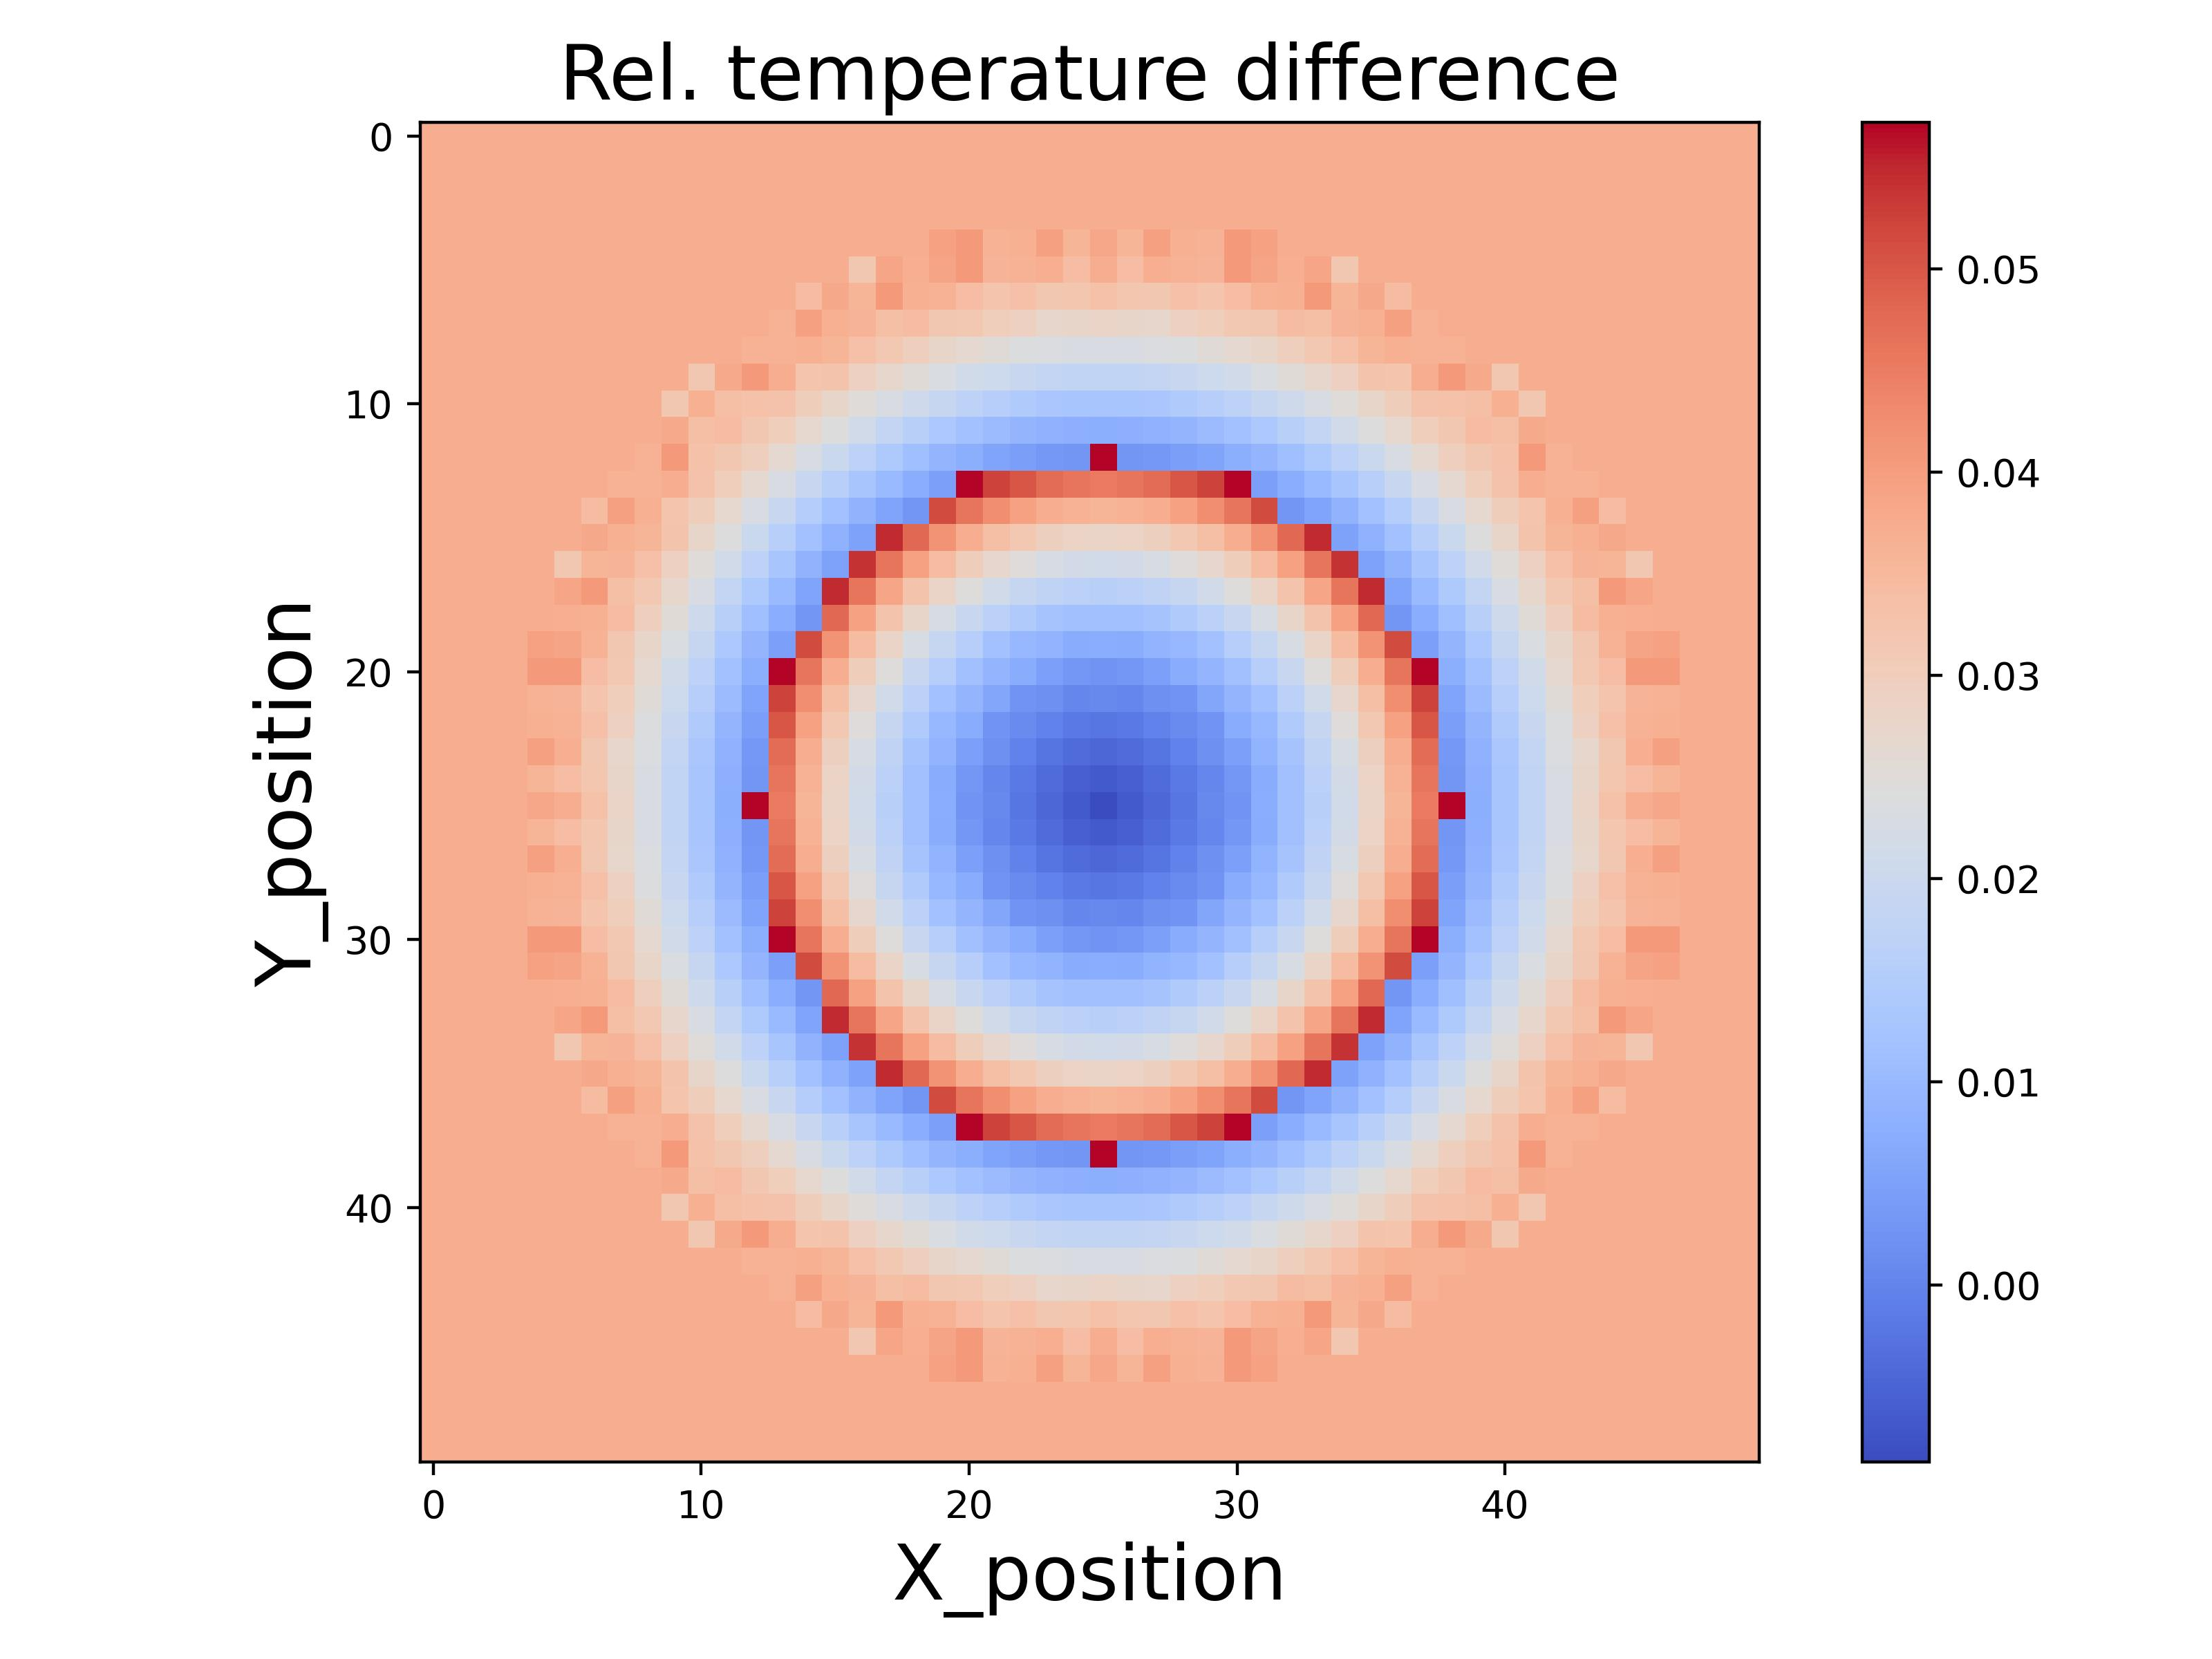
\includegraphics[width=\textwidth]{figures/raw_data/33/linear/T_bias.jpg}
            \subcaption{Model 9}
        \end{subfigure}
    \end{minipage}
    \caption{Temperature difference of linear model}  
\end{figure}
\begin{figure}[p]
    \centering
    \begin{minipage}{\textwidth}
        \centering
        \begin{subfigure}{0.325\textwidth}
            \centering
            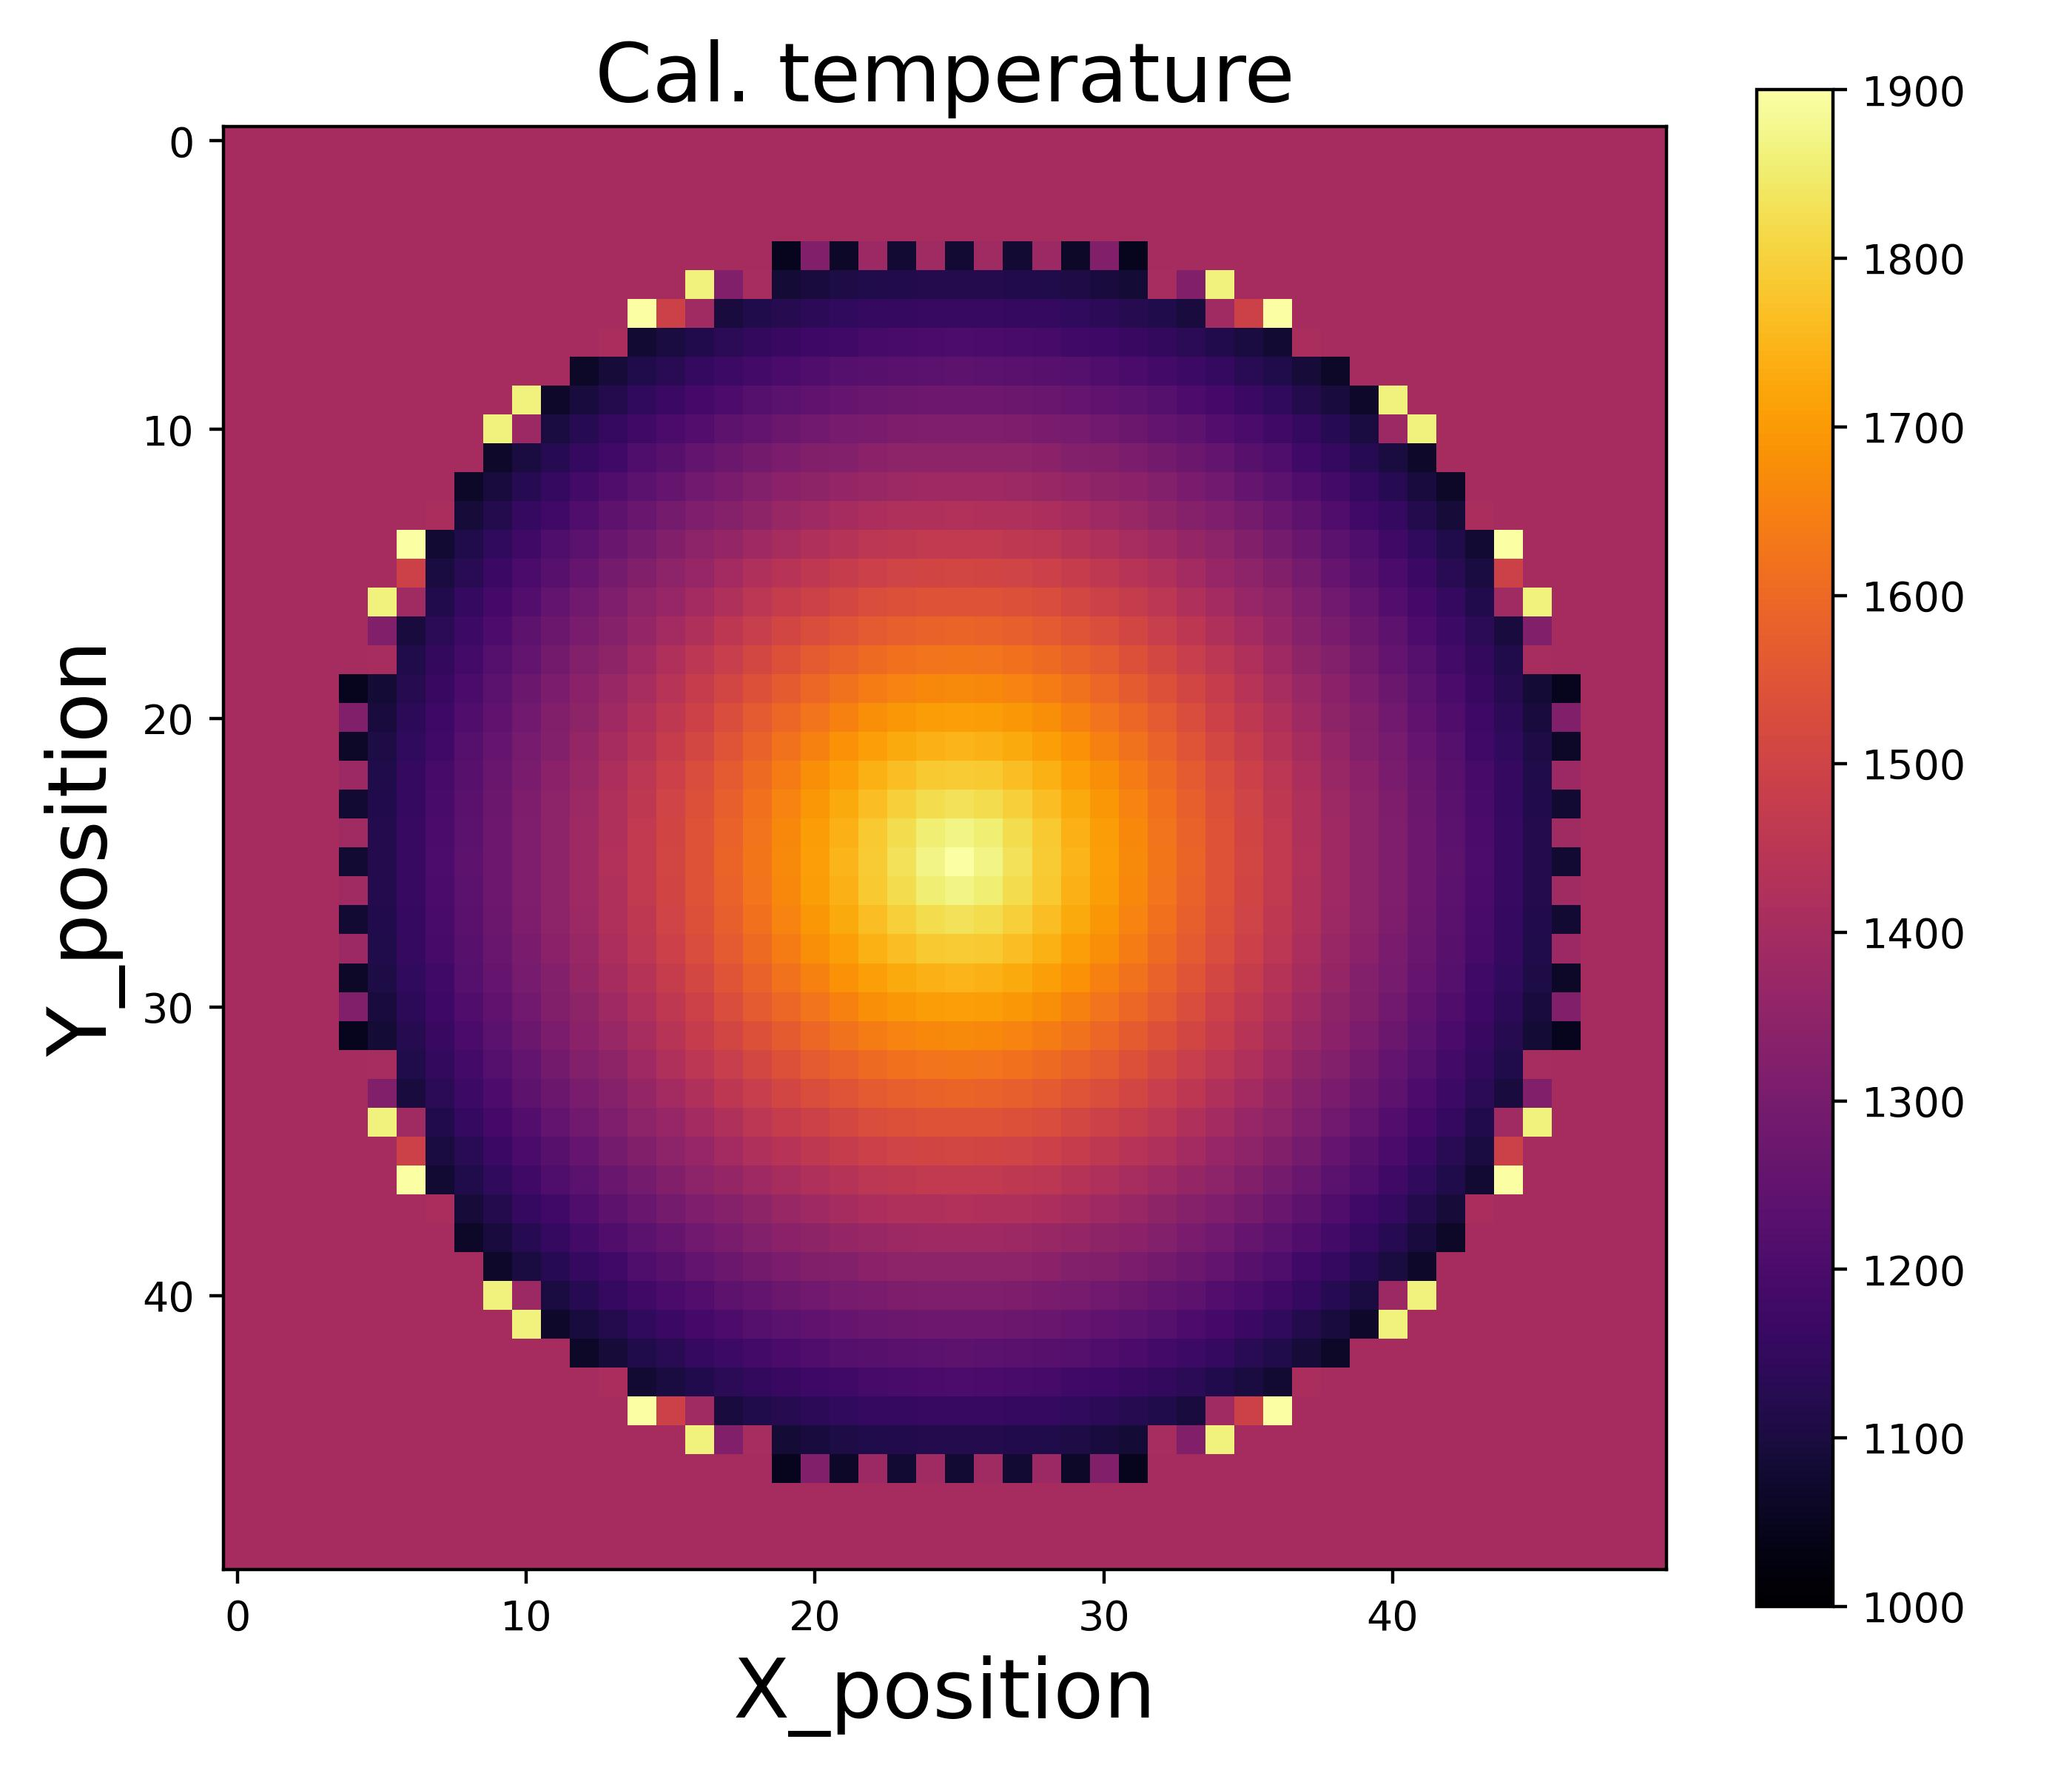
\includegraphics[width=\textwidth]{figures/raw_data/0/linear/T_cal.jpg}
            \subcaption{Black body material}
        \end{subfigure}
        \begin{subfigure}{0.325\textwidth}
            \centering
            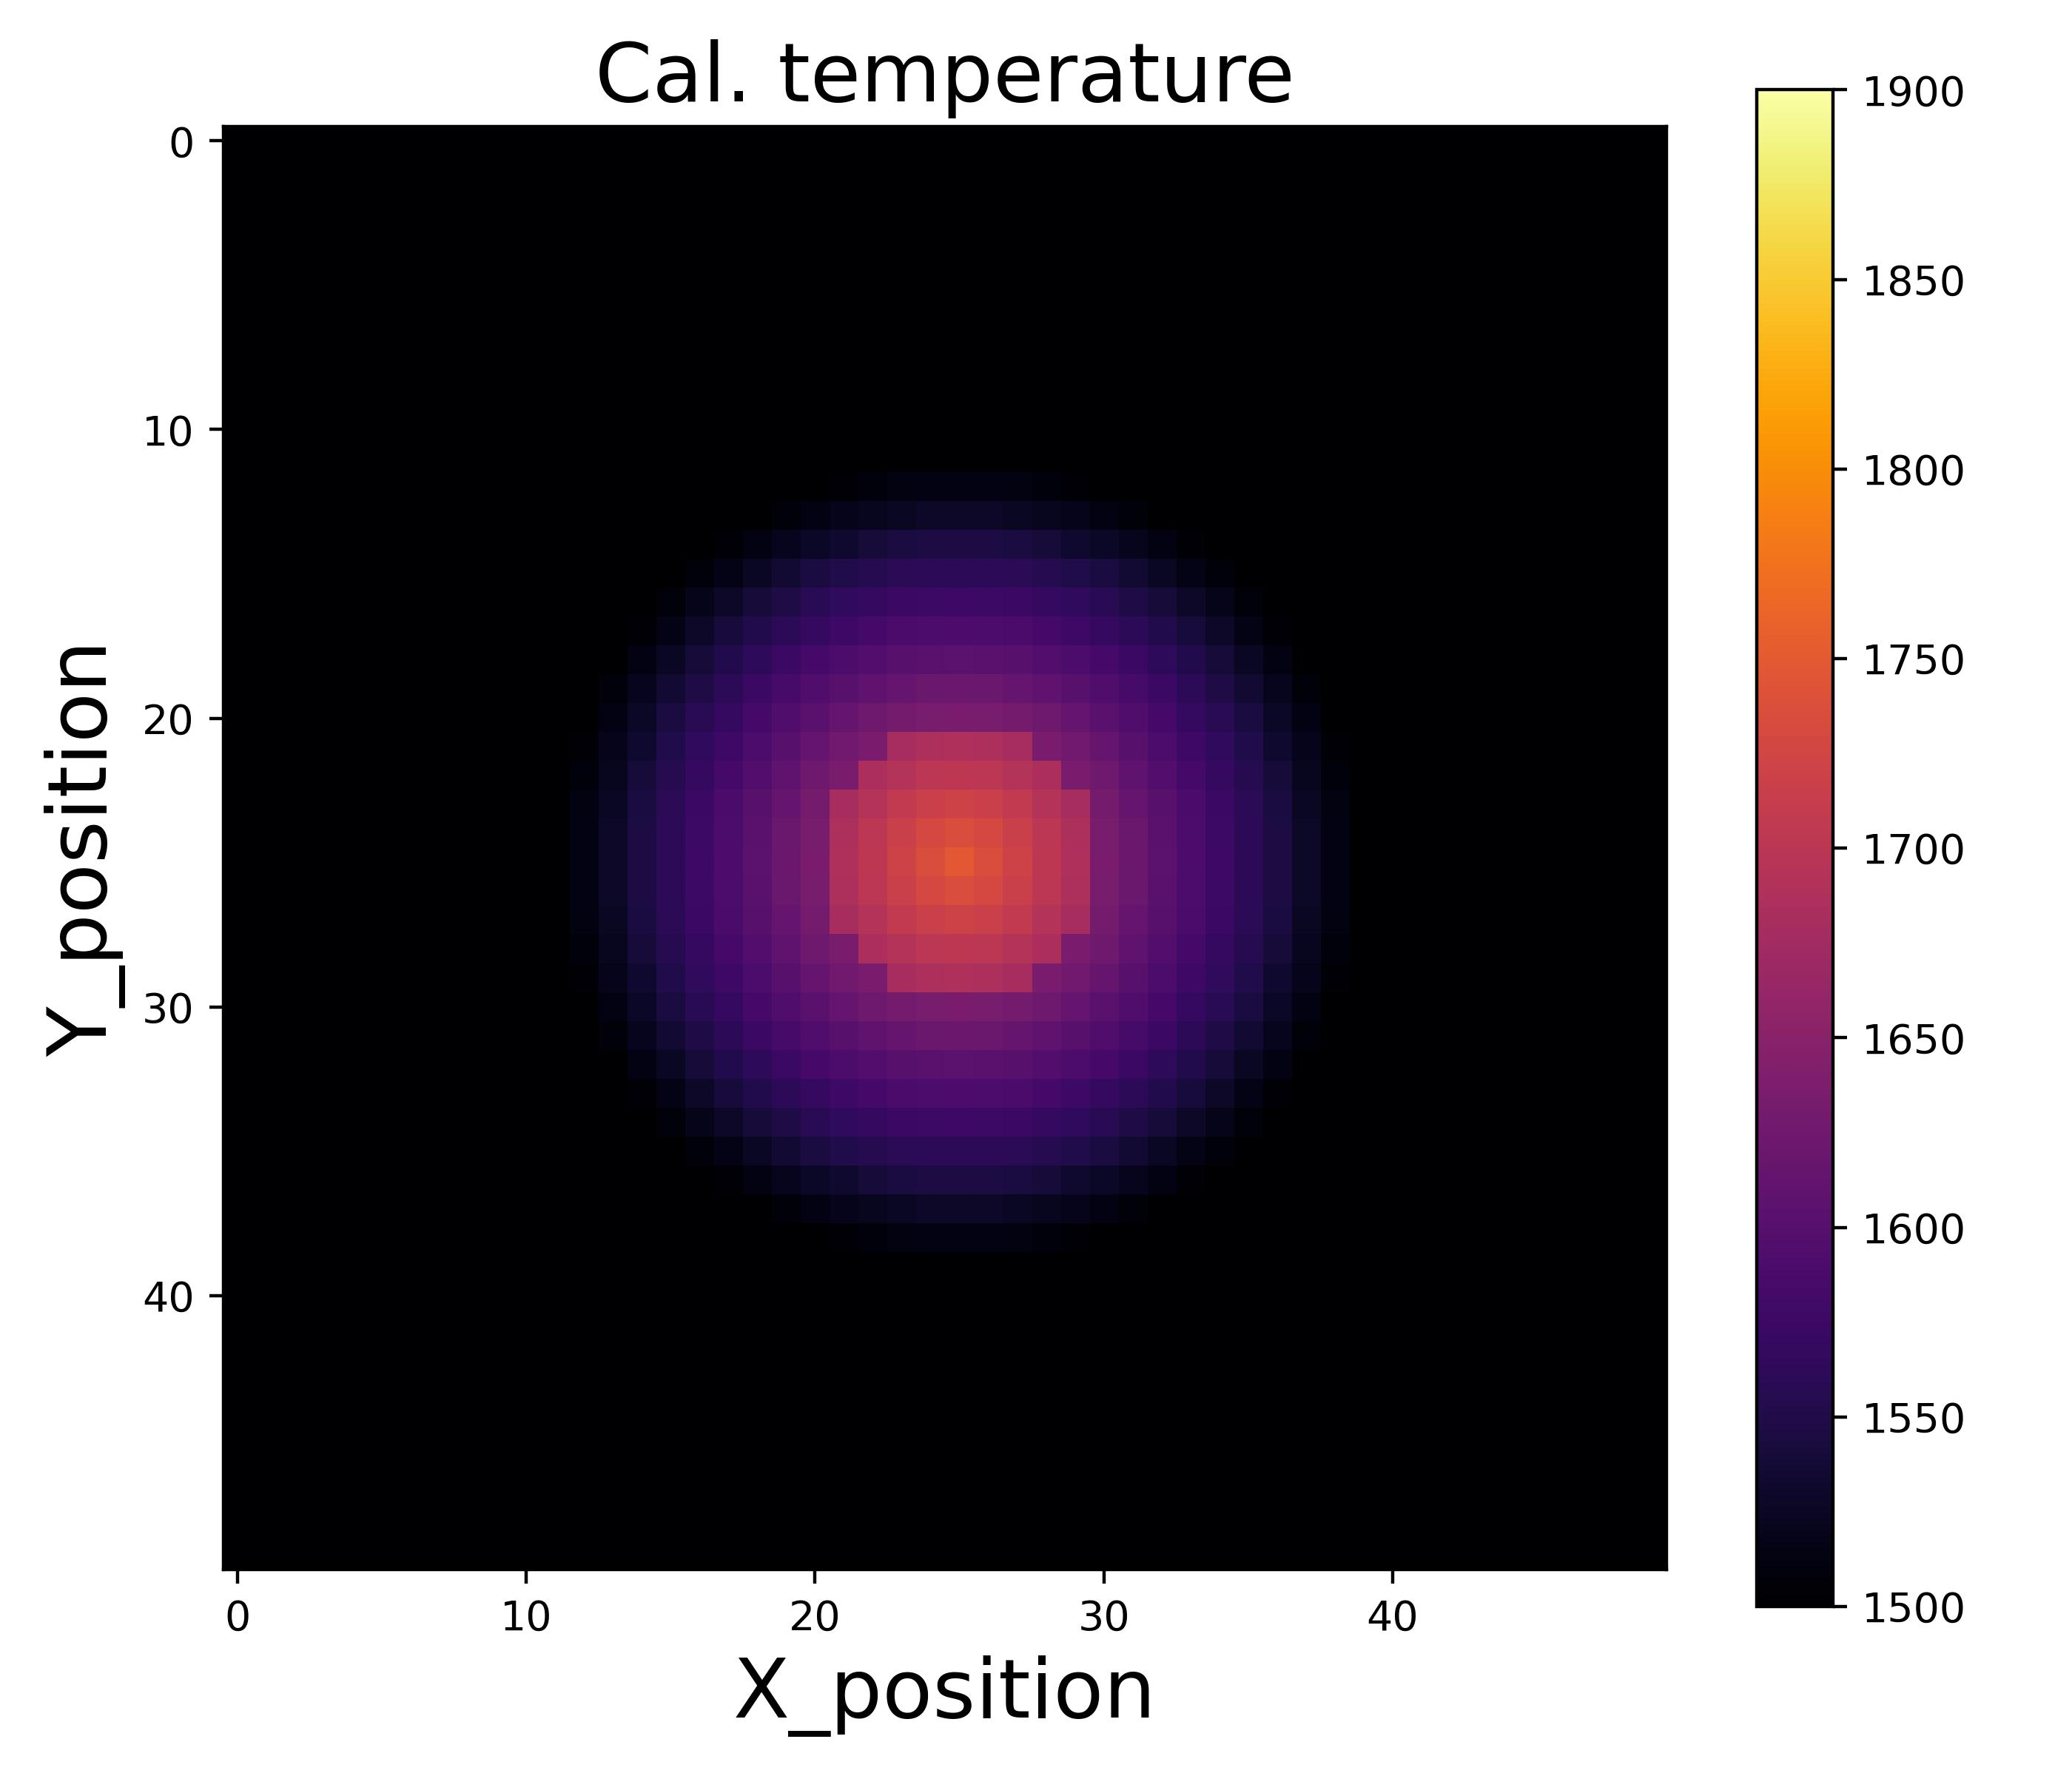
\includegraphics[width=\textwidth]{figures/raw_data/5/linear/T_cal.jpg}
            \subcaption{Real iron data}
        \end{subfigure}
        \begin{subfigure}{0.325\textwidth}
            \centering
            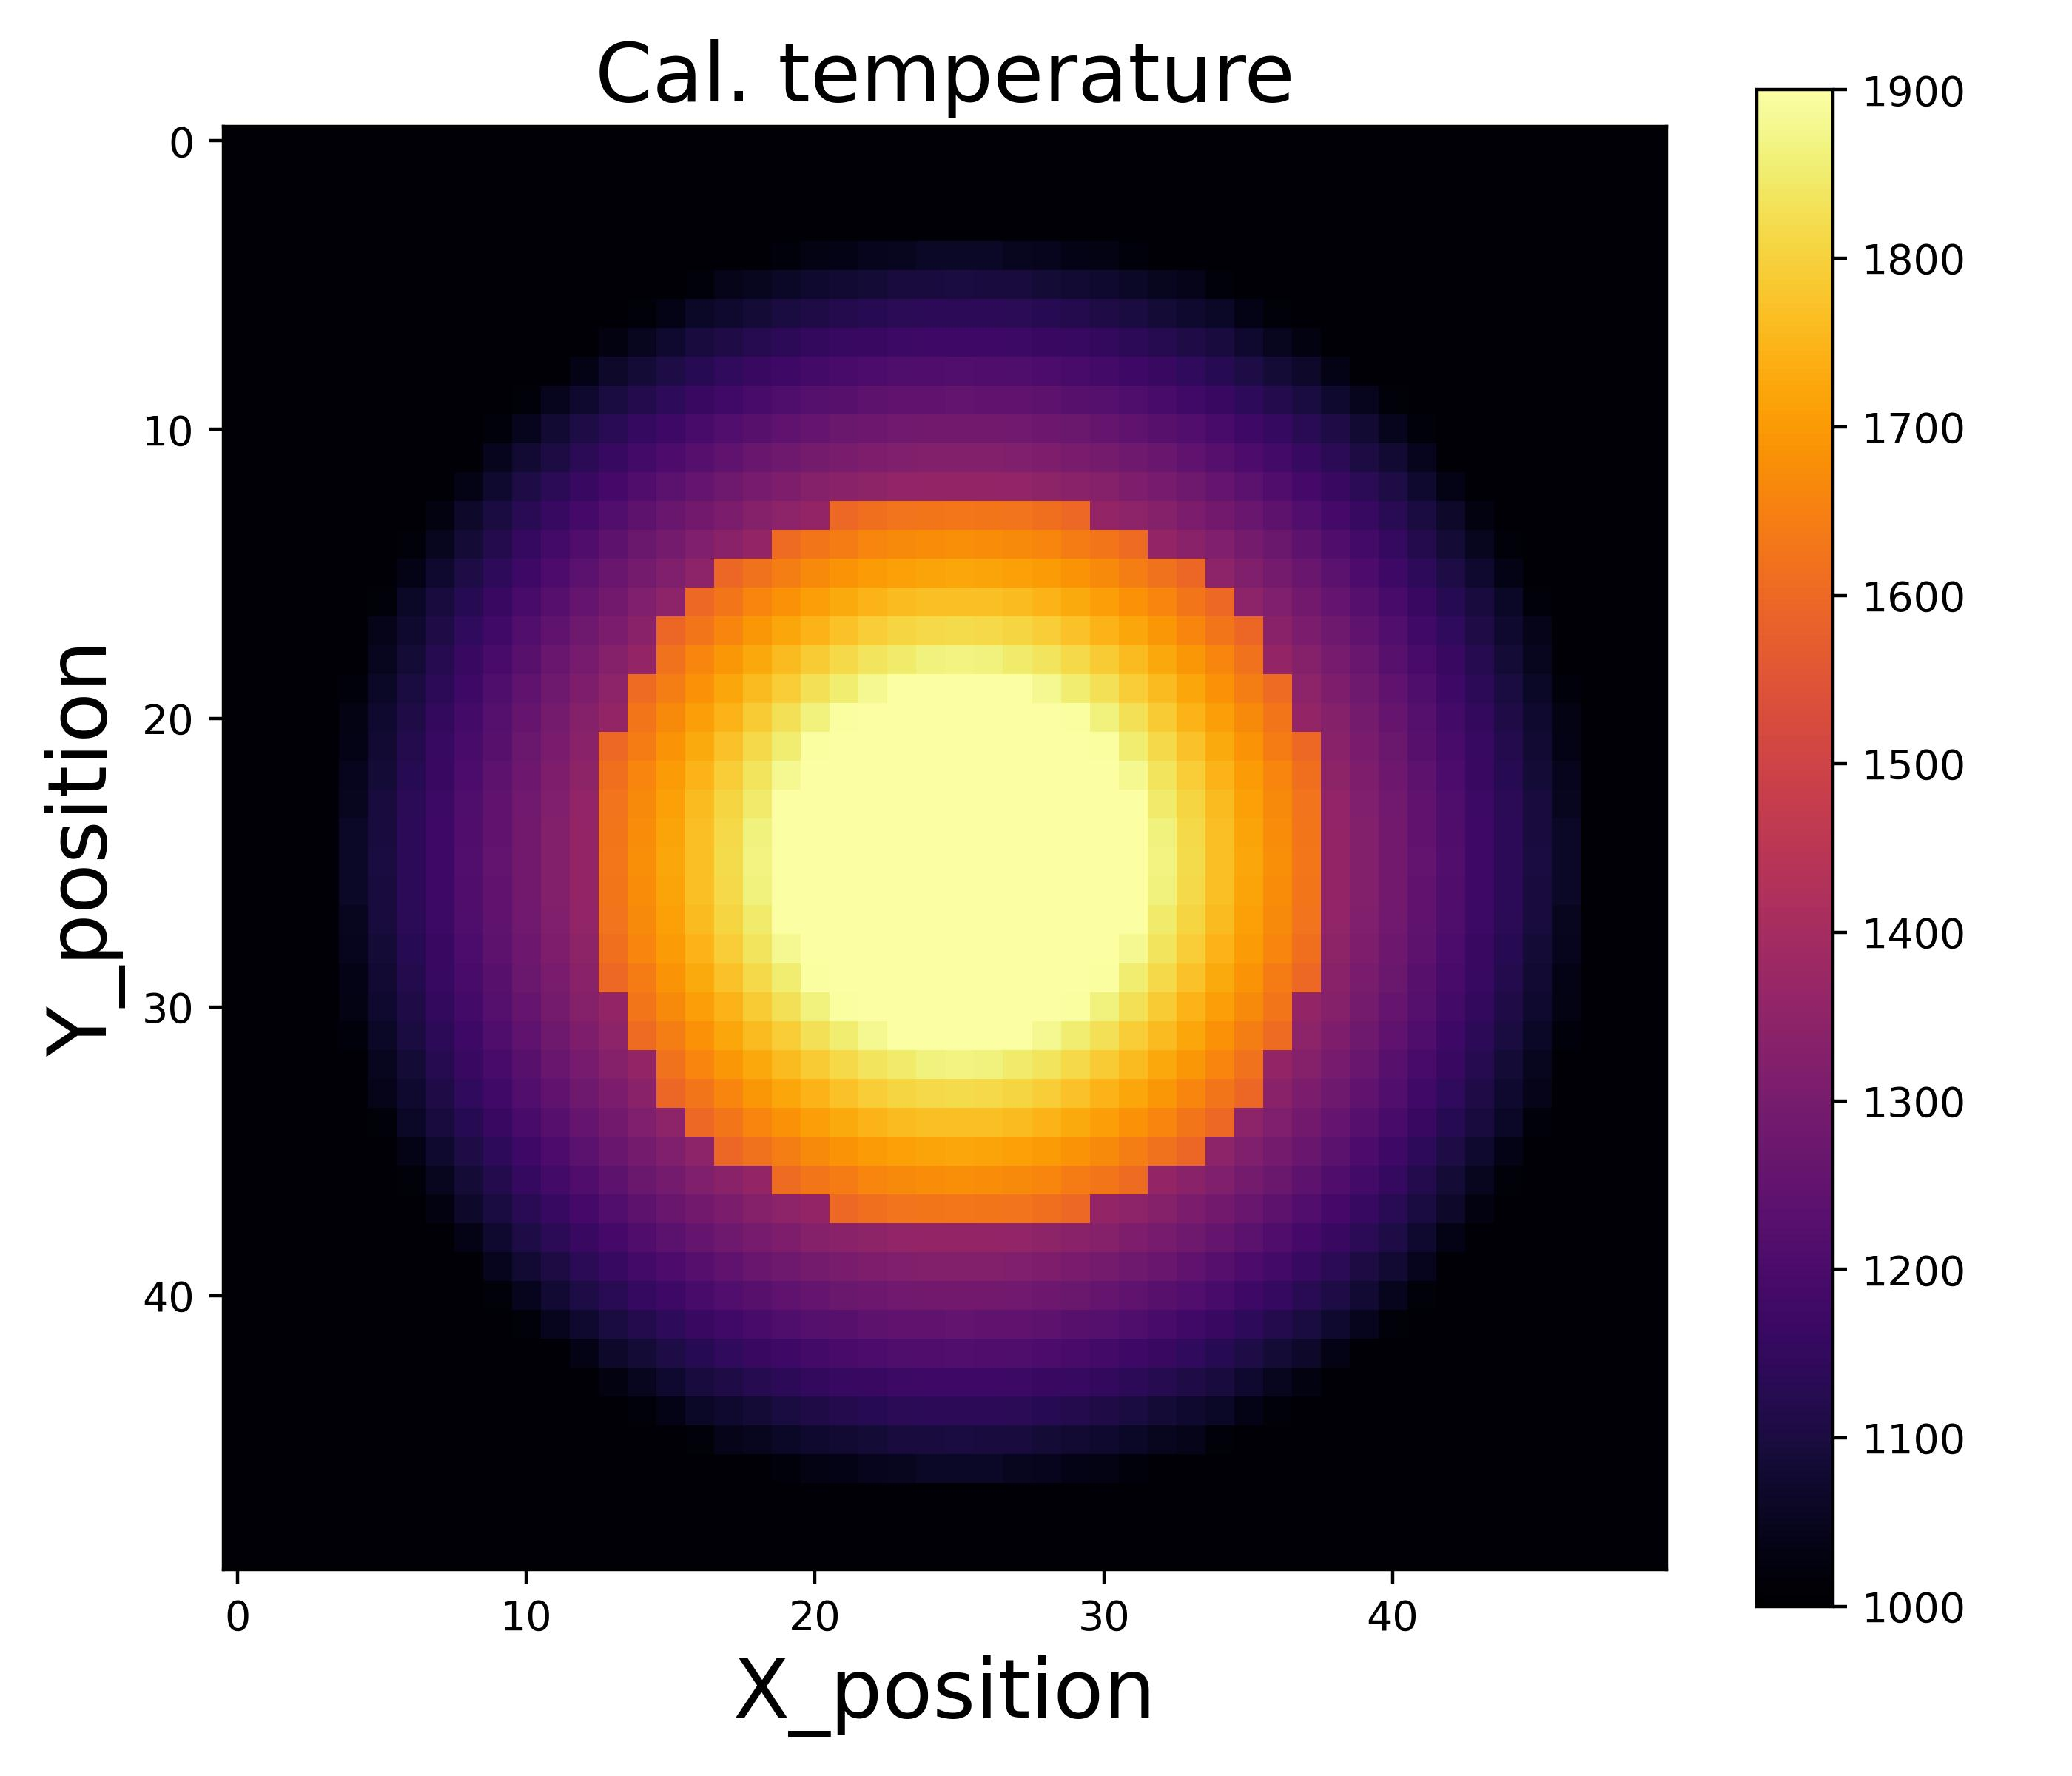
\includegraphics[width=\textwidth]{figures/raw_data/21/linear/T_cal.jpg}
            \subcaption{Model 1}
        \end{subfigure}
    \end{minipage}\\
    \begin{minipage}{\textwidth}
        \centering
        \begin{subfigure}{0.325\textwidth}
            \centering
            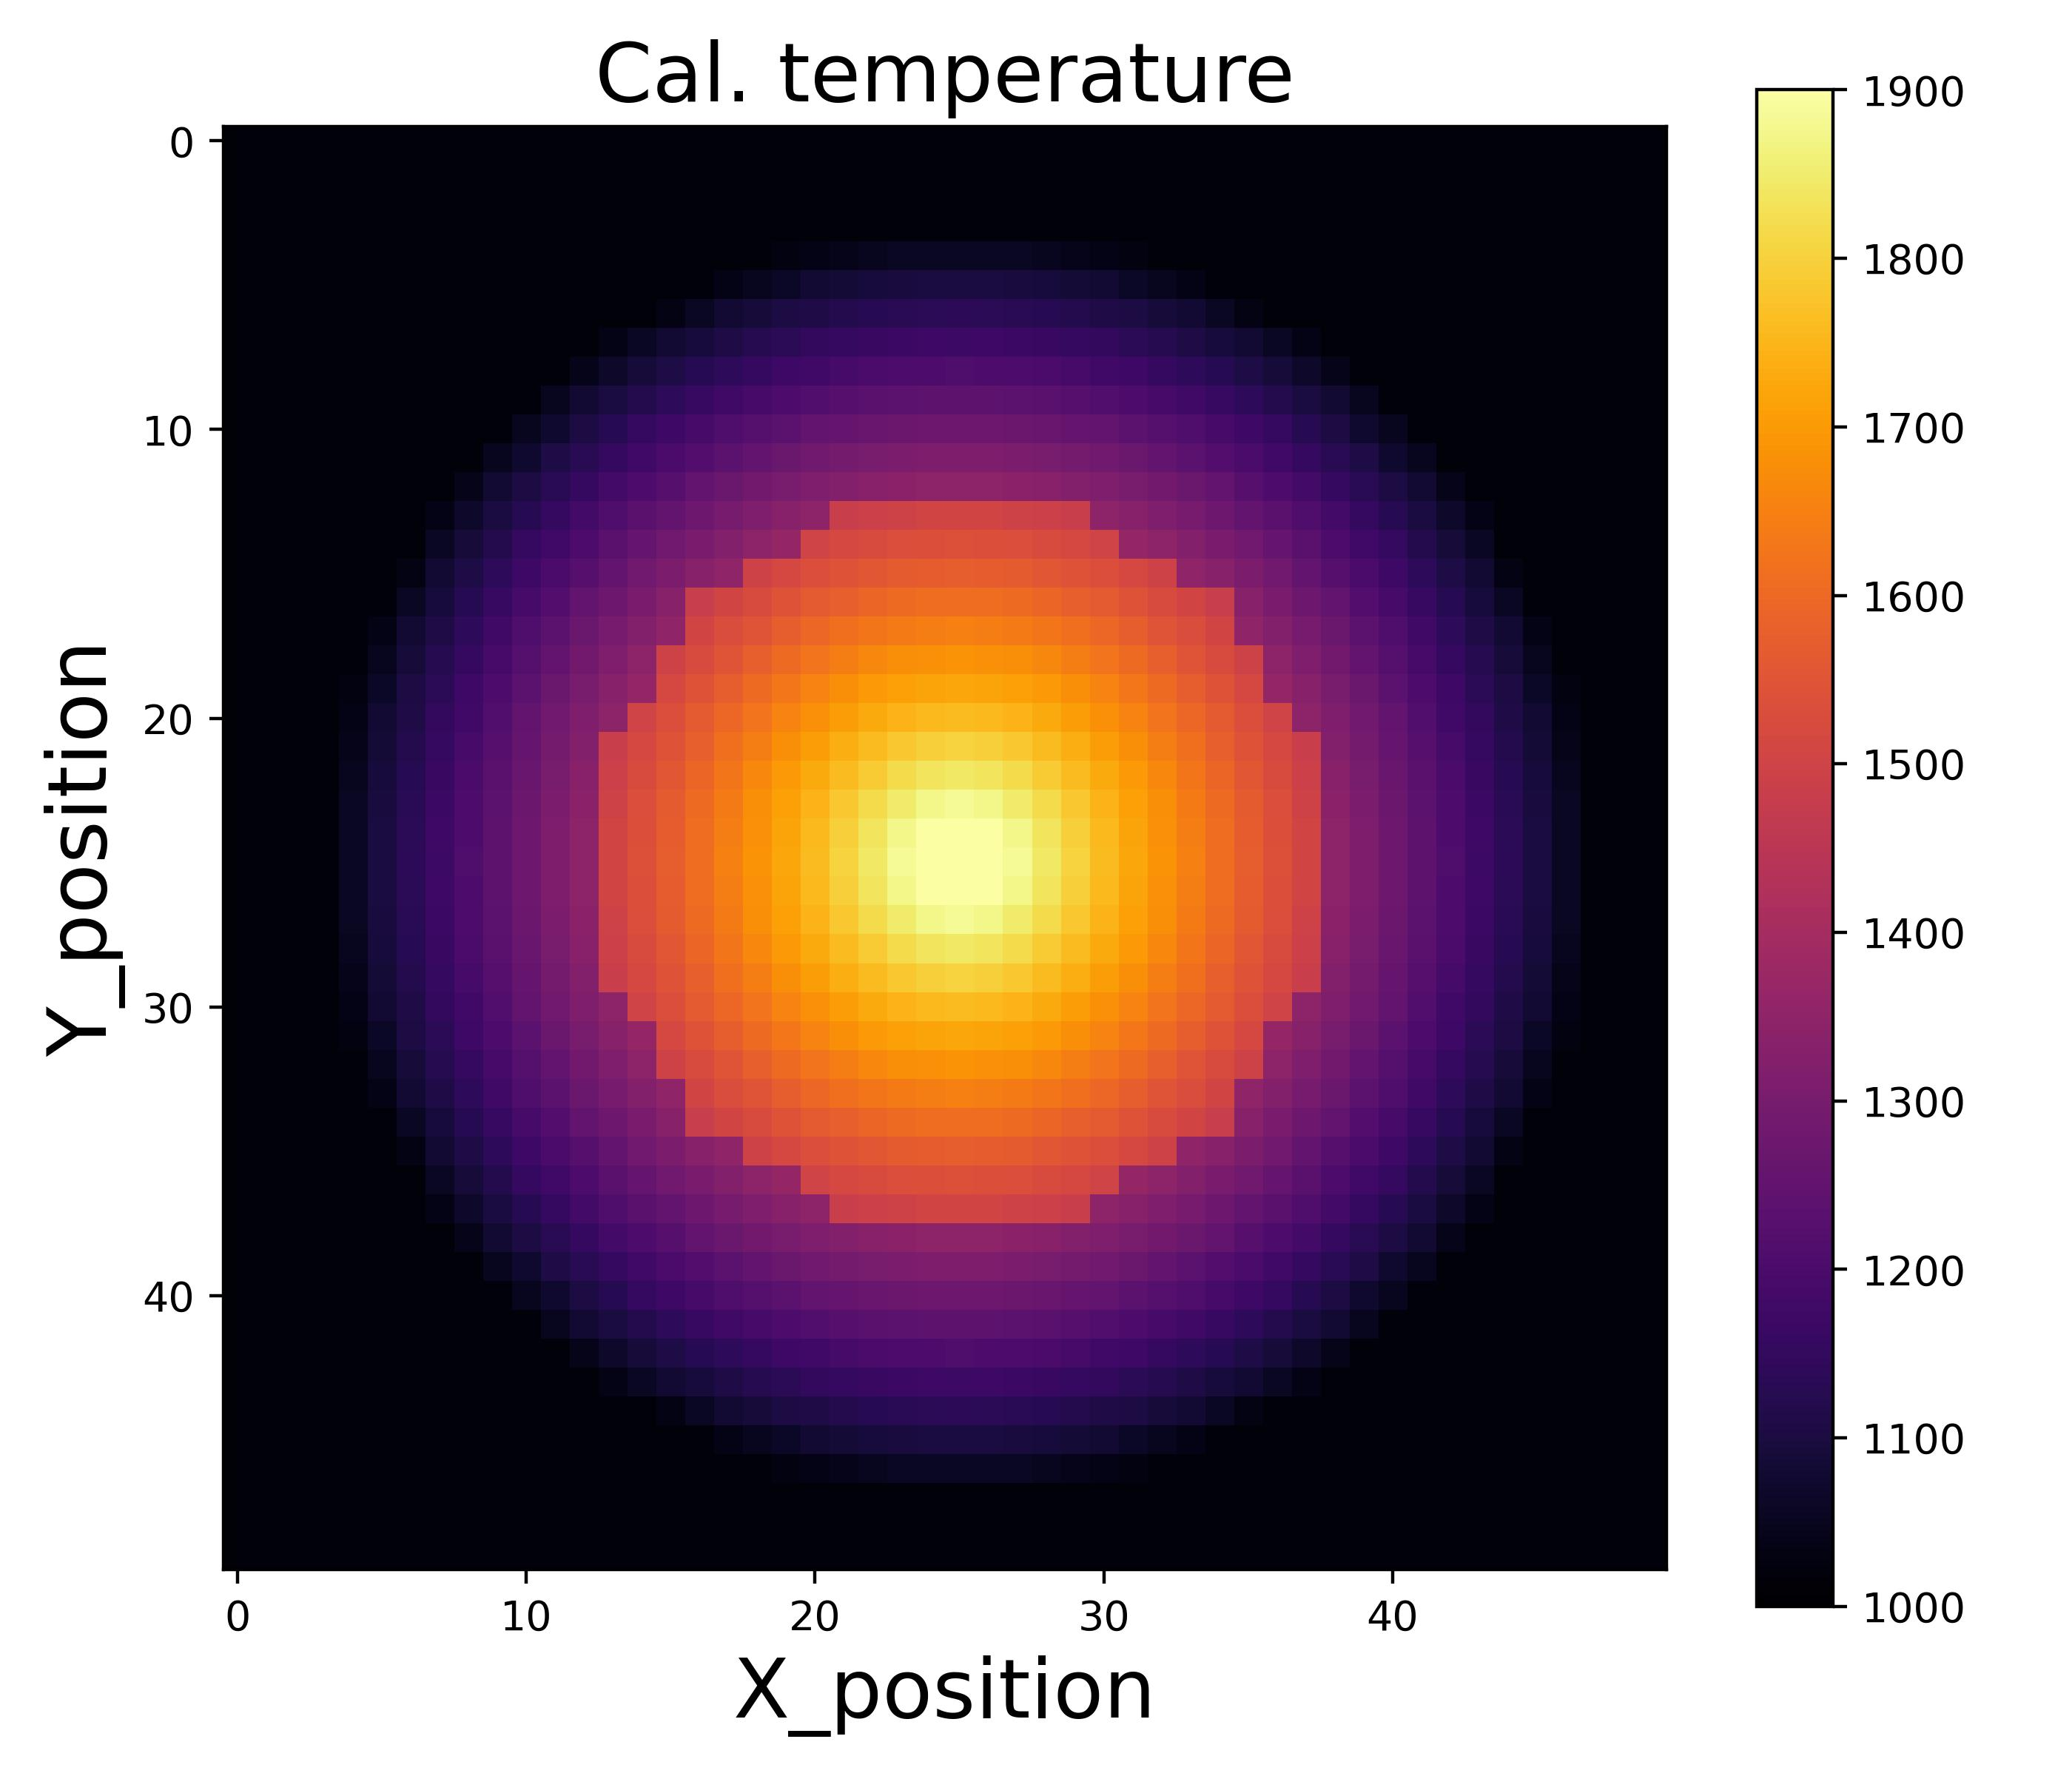
\includegraphics[width=\textwidth]{figures/raw_data/22/linear/T_cal.jpg}
            \subcaption{Model 2}
        \end{subfigure}
        \begin{subfigure}{0.325\textwidth}
            \centering
            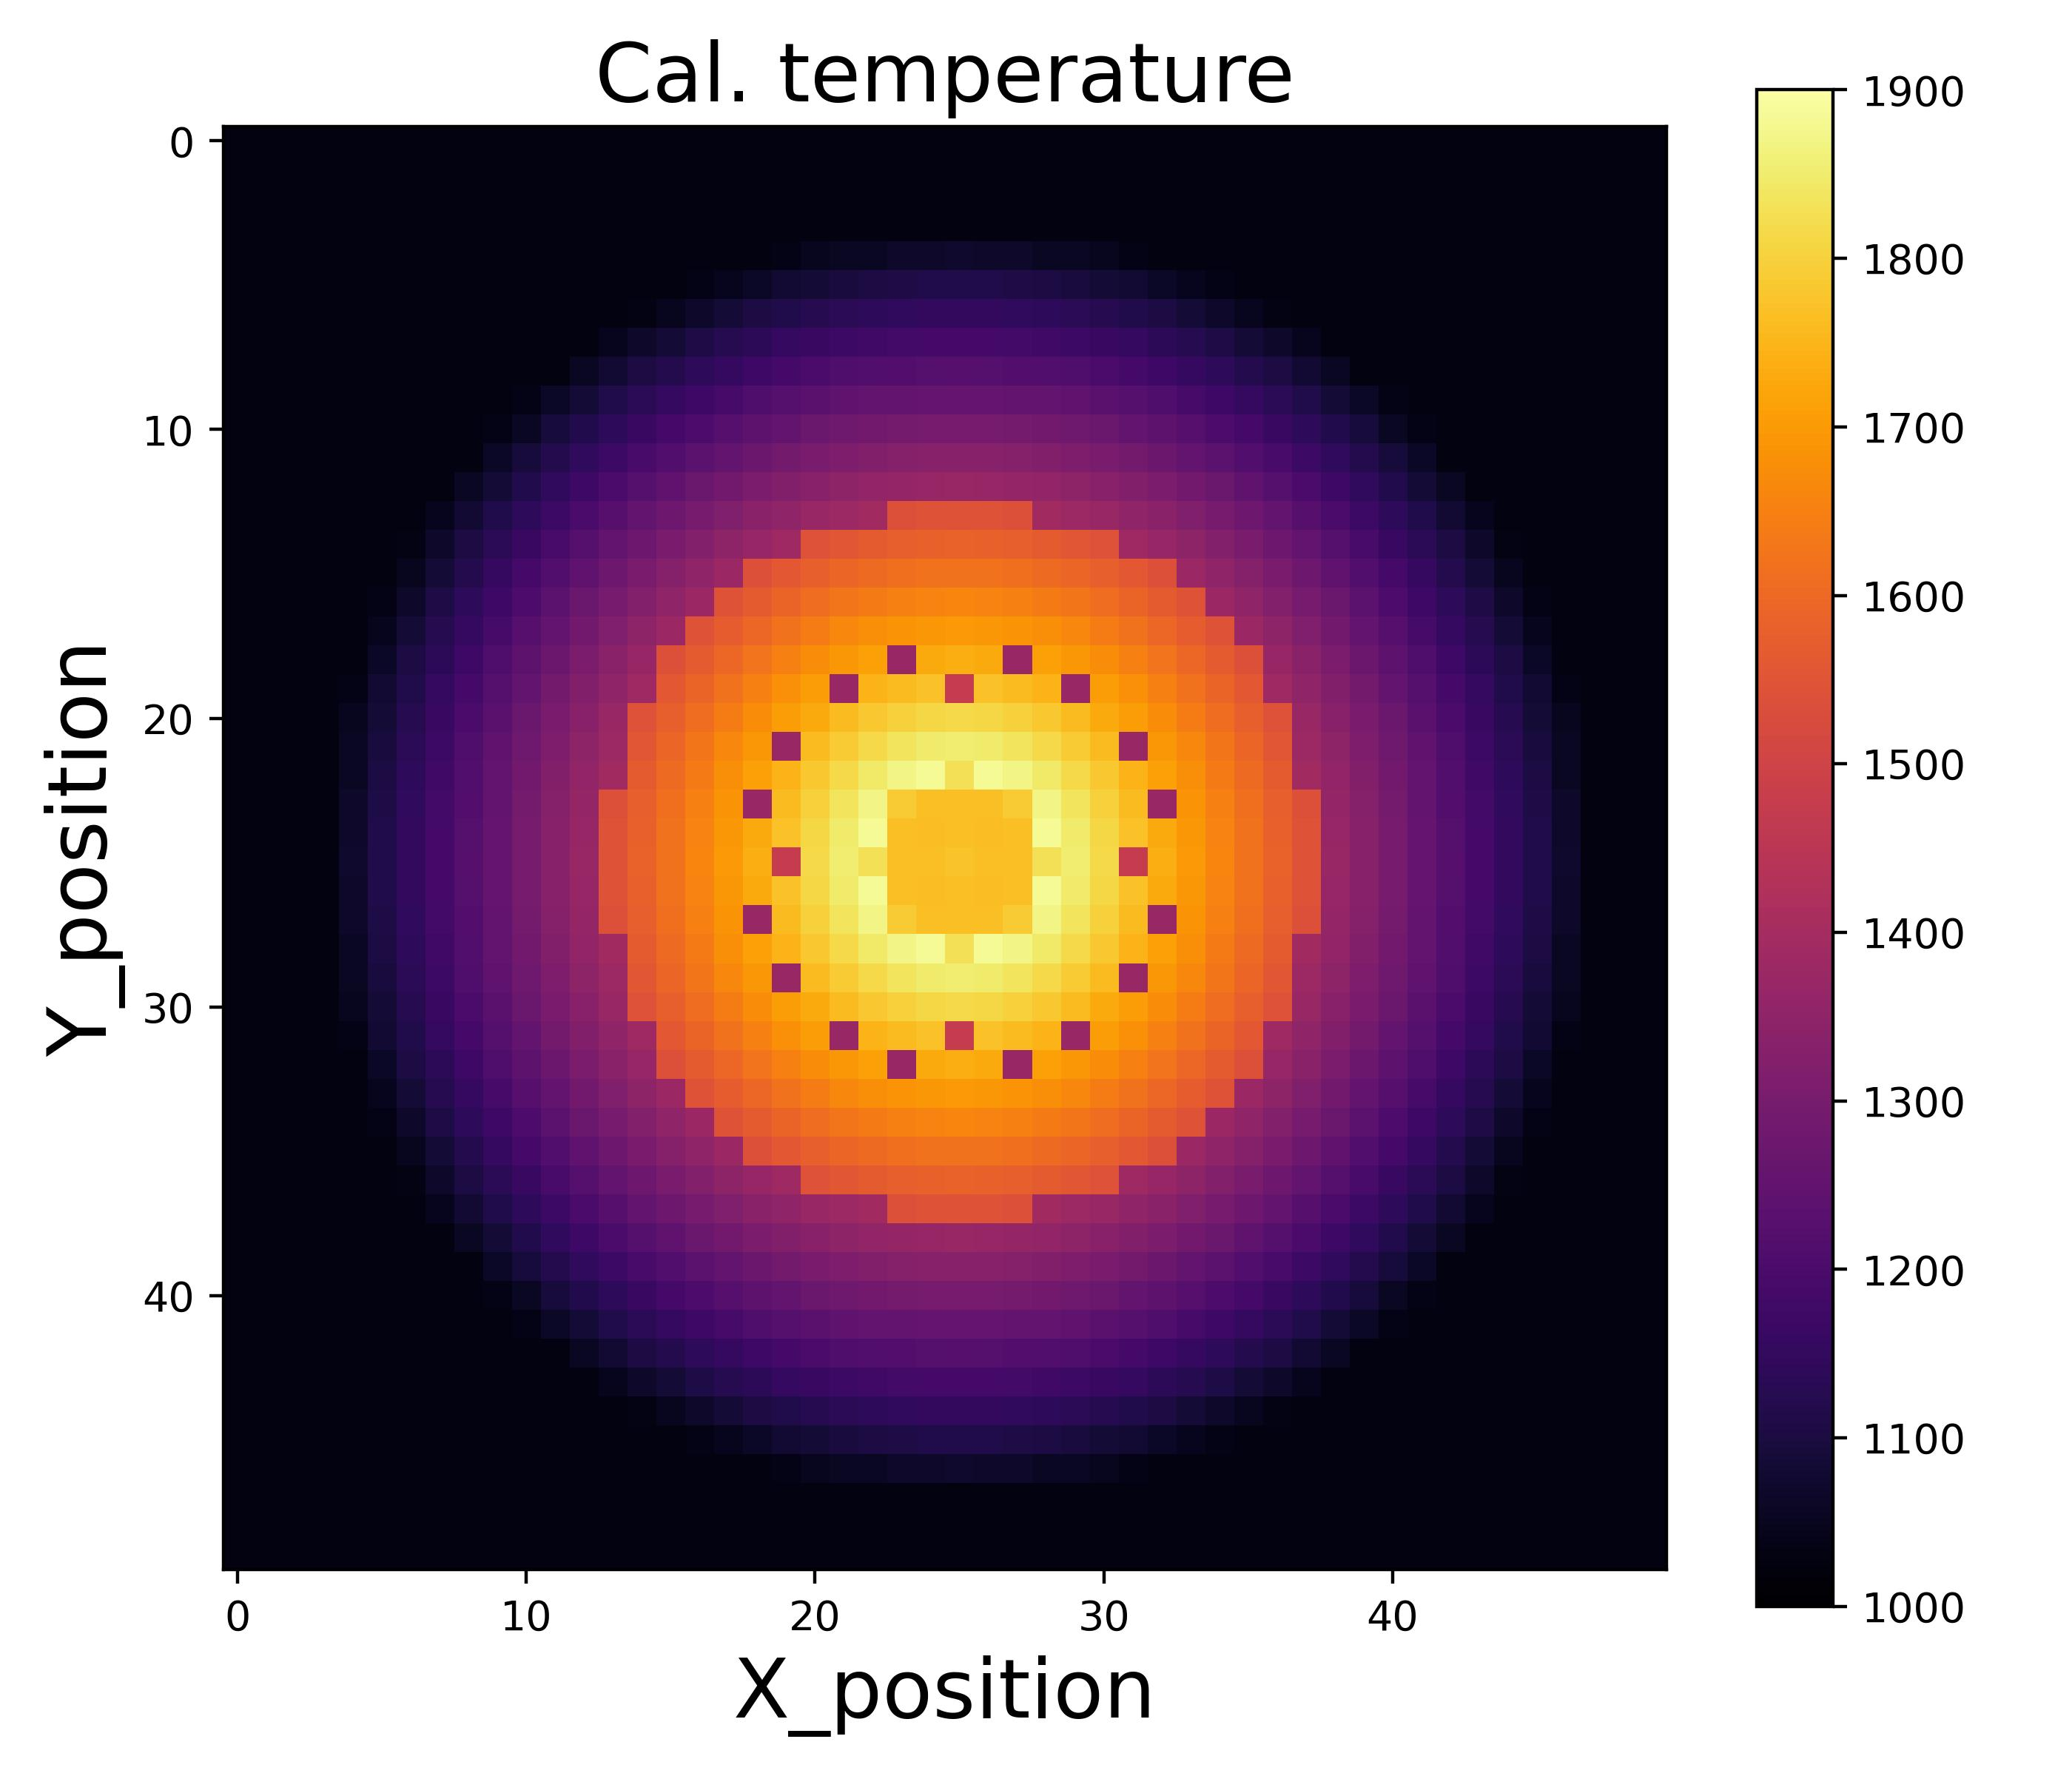
\includegraphics[width=\textwidth]{figures/raw_data/23/linear/T_cal.jpg}
            \subcaption{Model 3}
        \end{subfigure}
        \begin{subfigure}{0.325\textwidth}
            \centering
            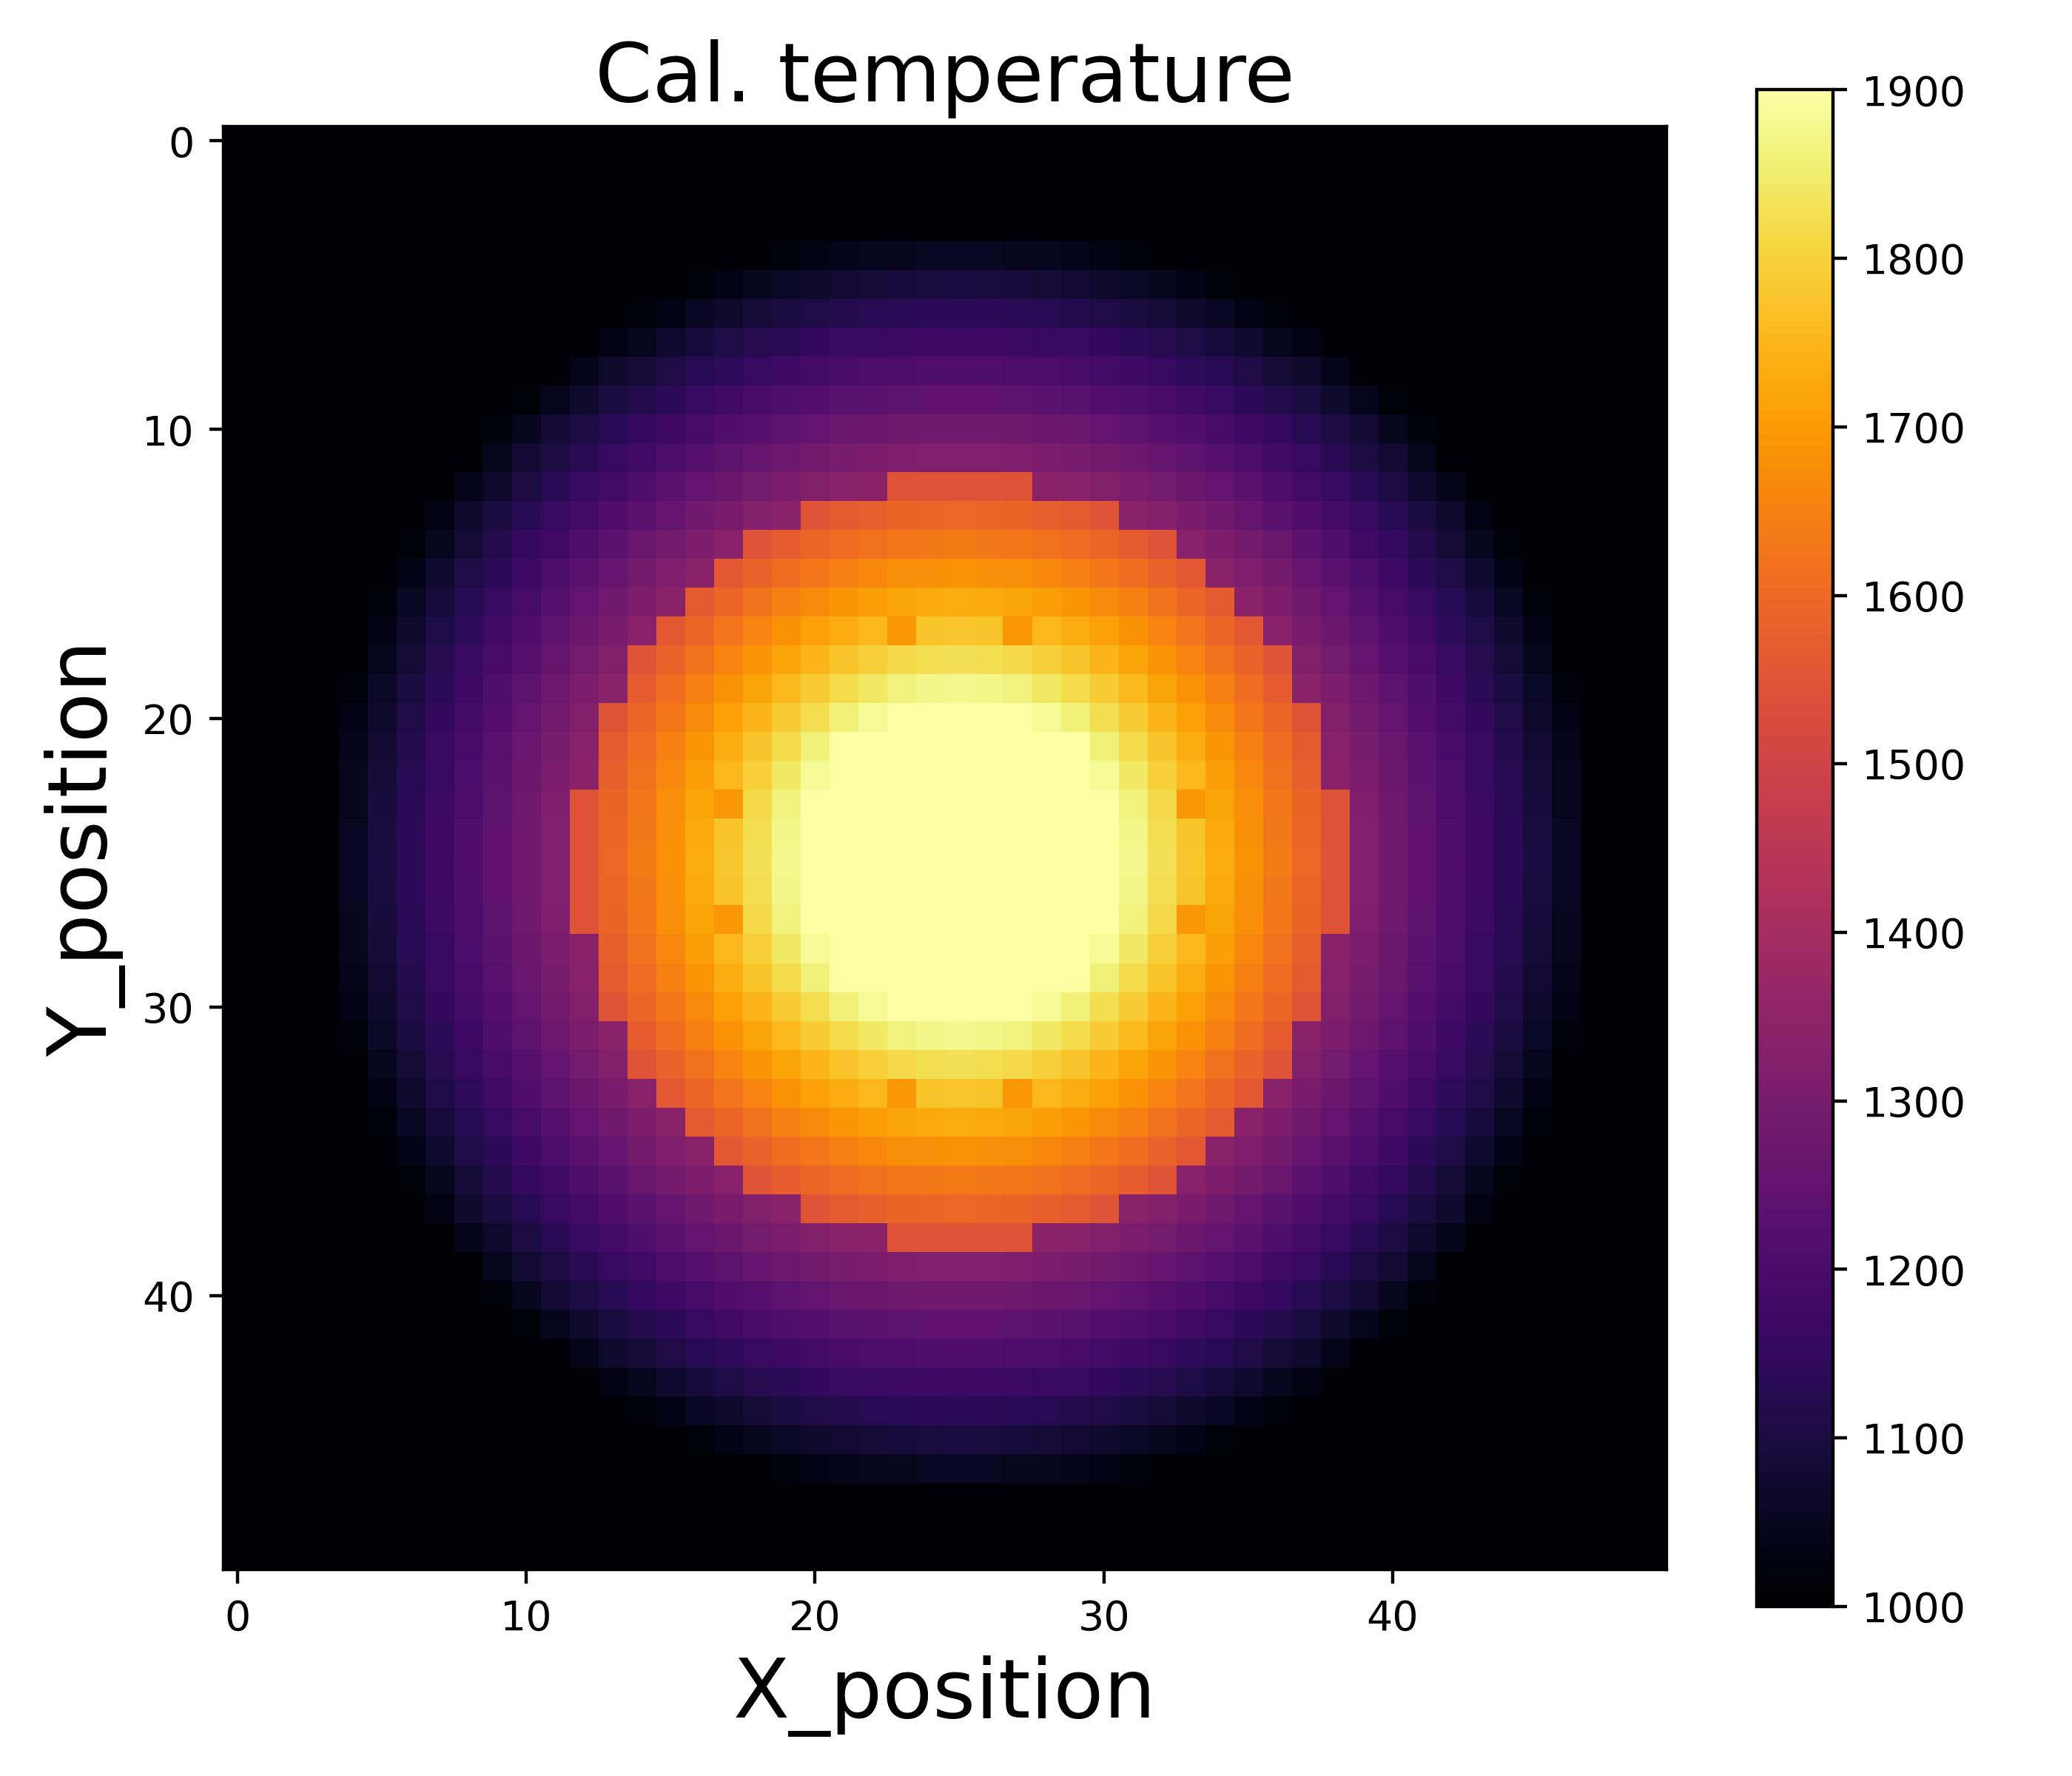
\includegraphics[width=\textwidth]{figures/raw_data/24/linear/T_cal.jpg}
            \subcaption{Model 4}
        \end{subfigure}
    \end{minipage}\\
    \begin{minipage}{\textwidth}
        \centering
        \begin{subfigure}{0.325\textwidth}
            \centering
            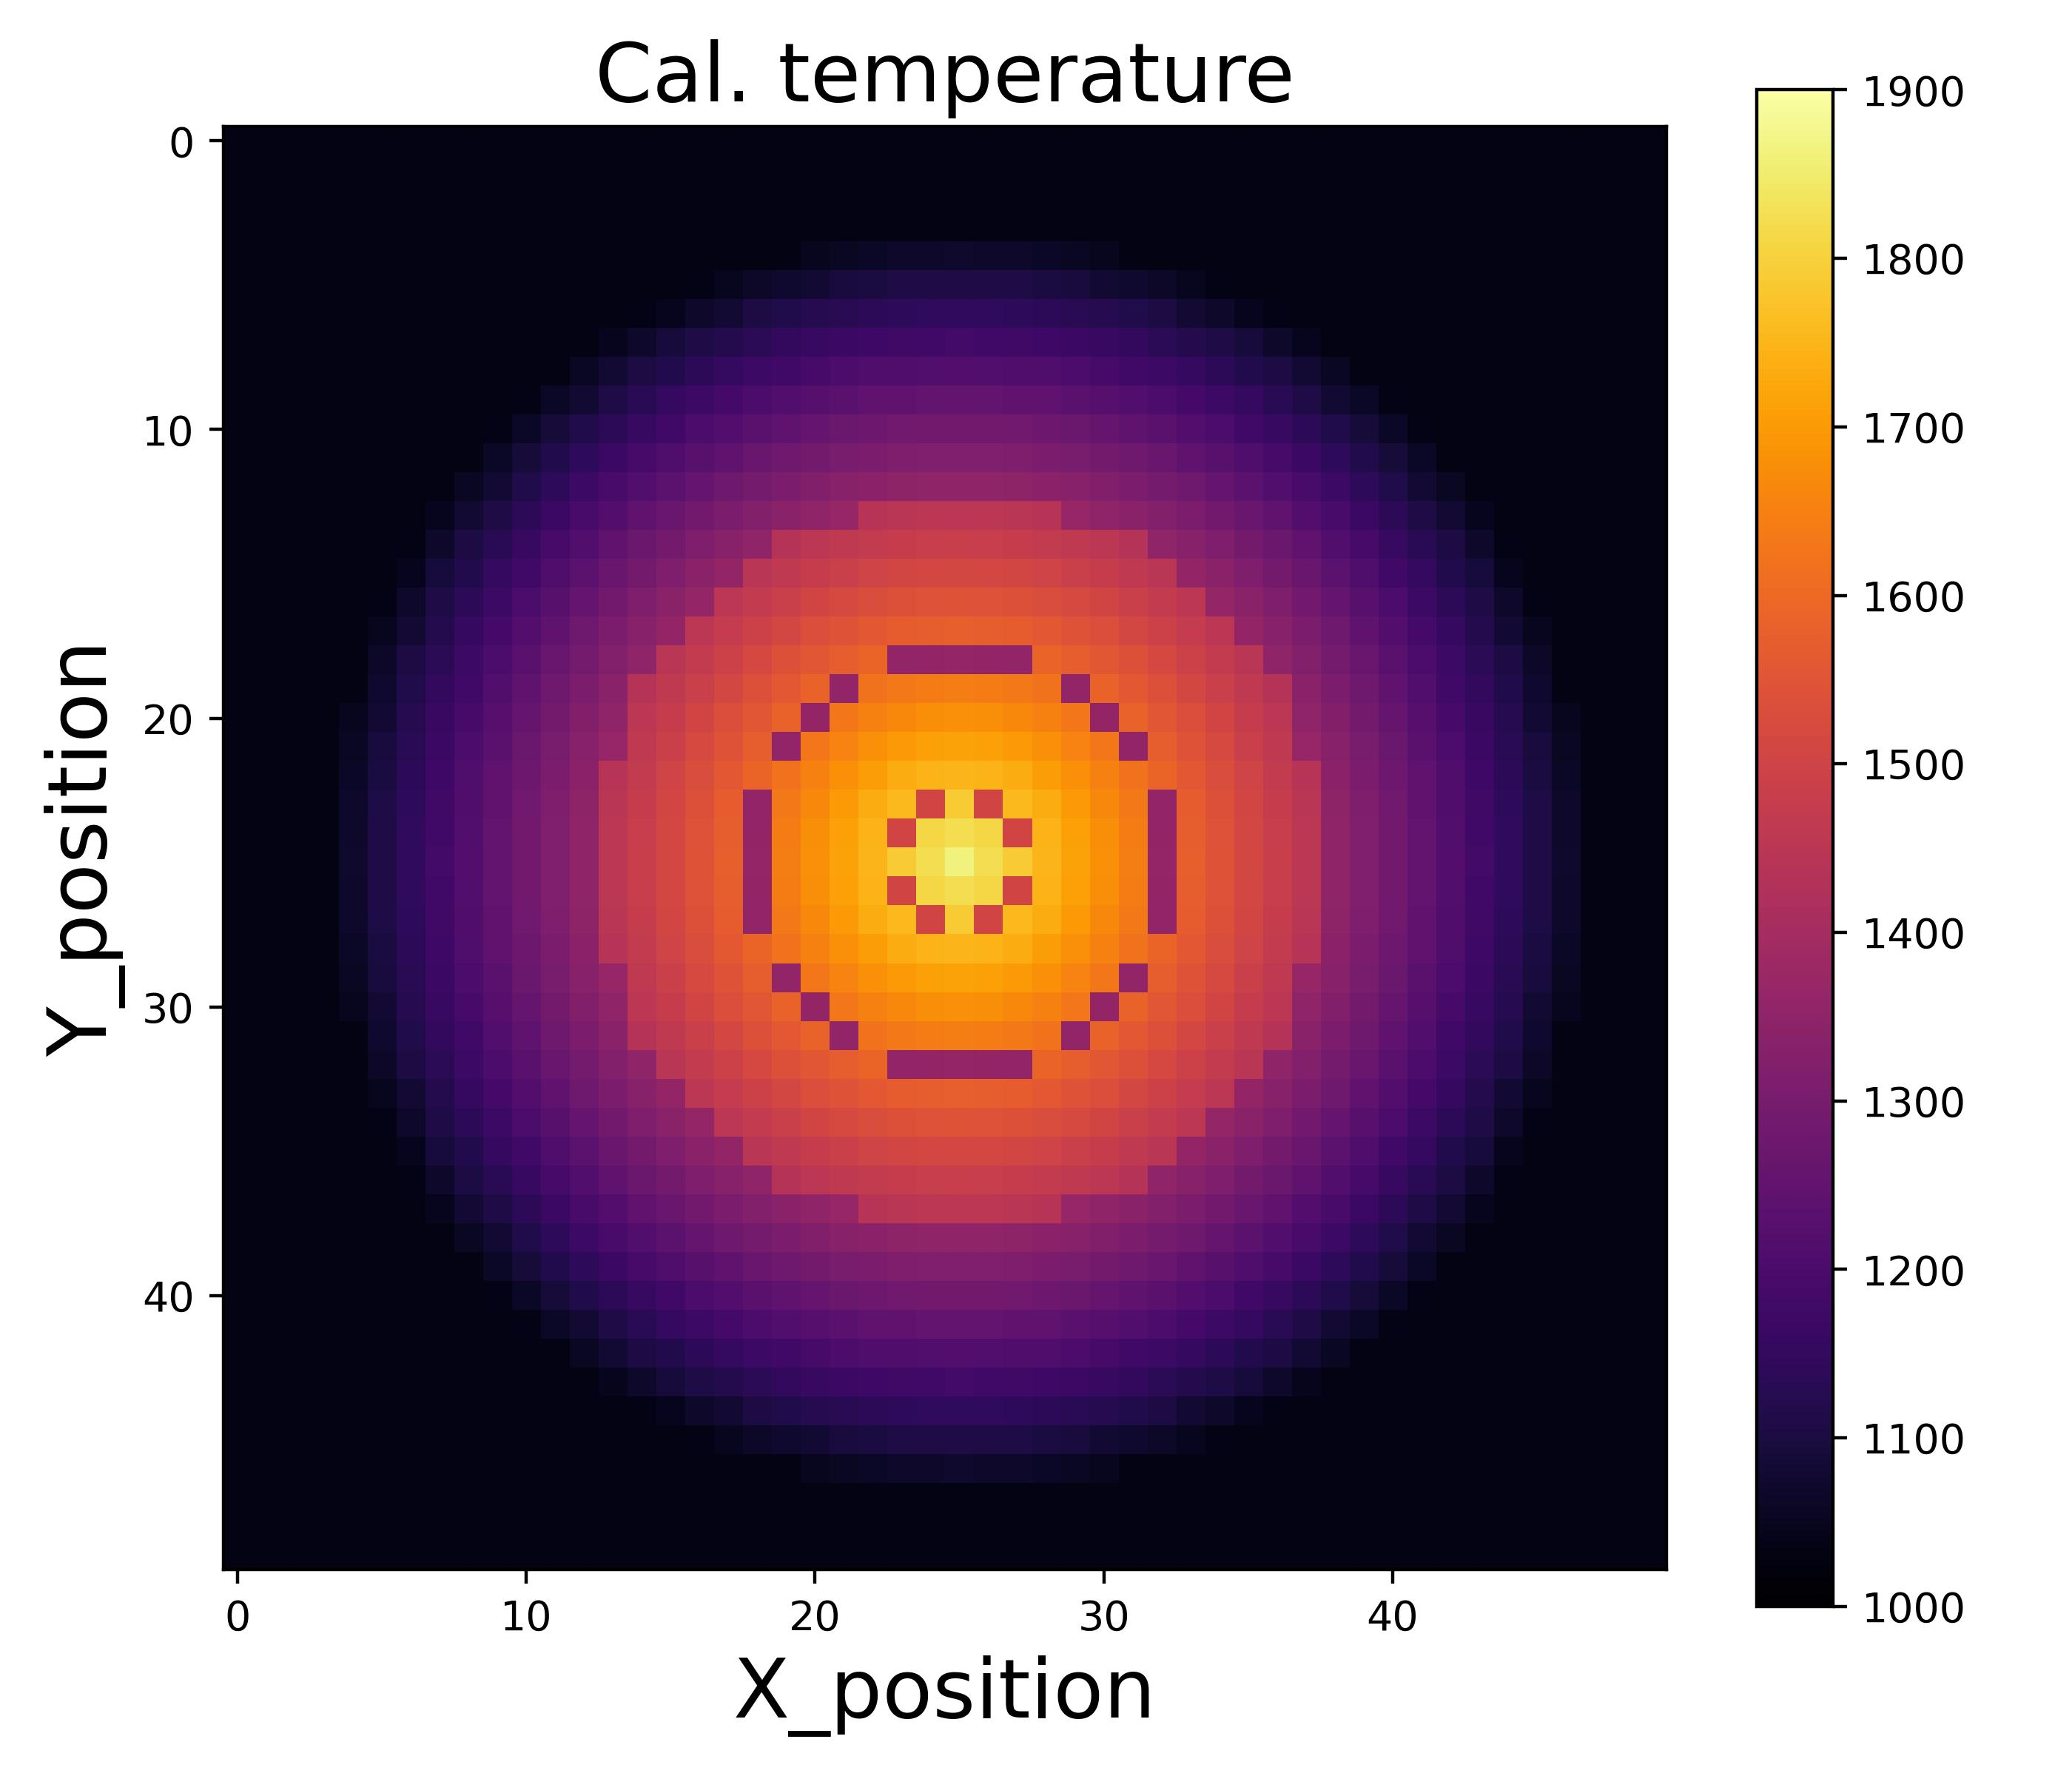
\includegraphics[width=\textwidth]{figures/raw_data/25/linear/T_cal.jpg}
            \subcaption{Model 5}
        \end{subfigure}
        \begin{subfigure}{0.325\textwidth}
            \centering
            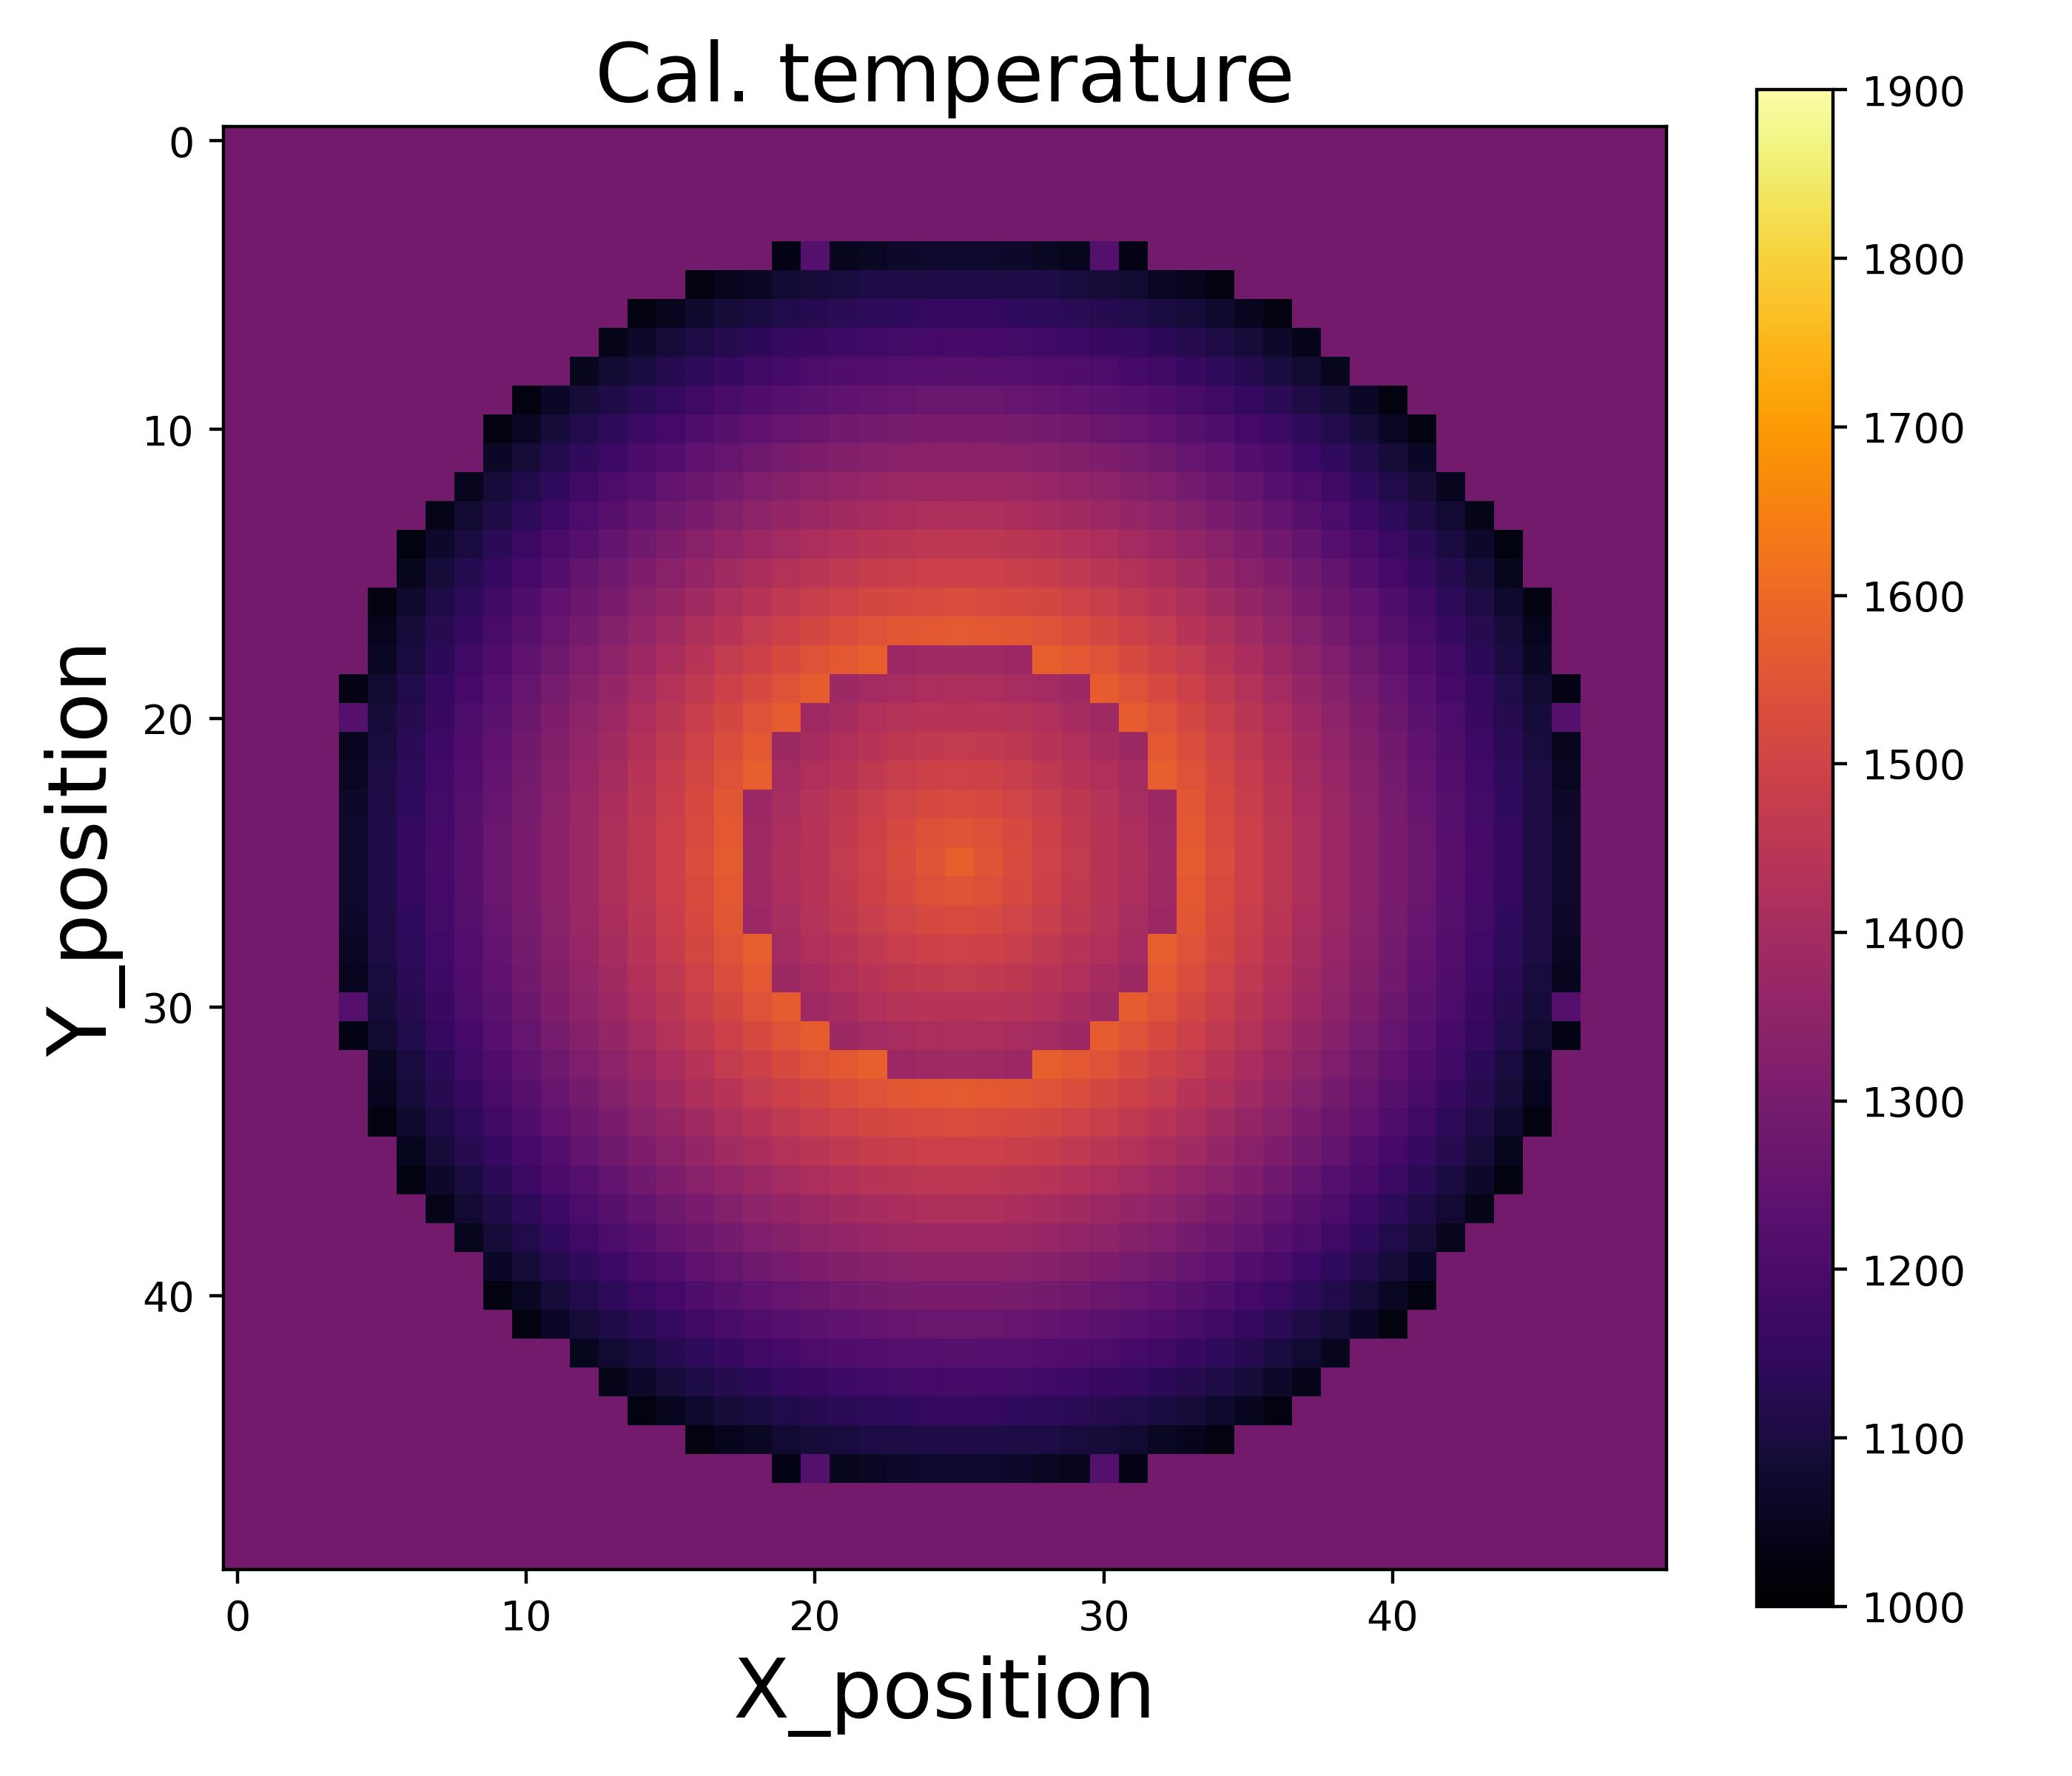
\includegraphics[width=\textwidth]{figures/raw_data/26/linear/T_cal.jpg}
            \subcaption{Model 6}
        \end{subfigure}
        \begin{subfigure}{0.325\textwidth}
            \centering
            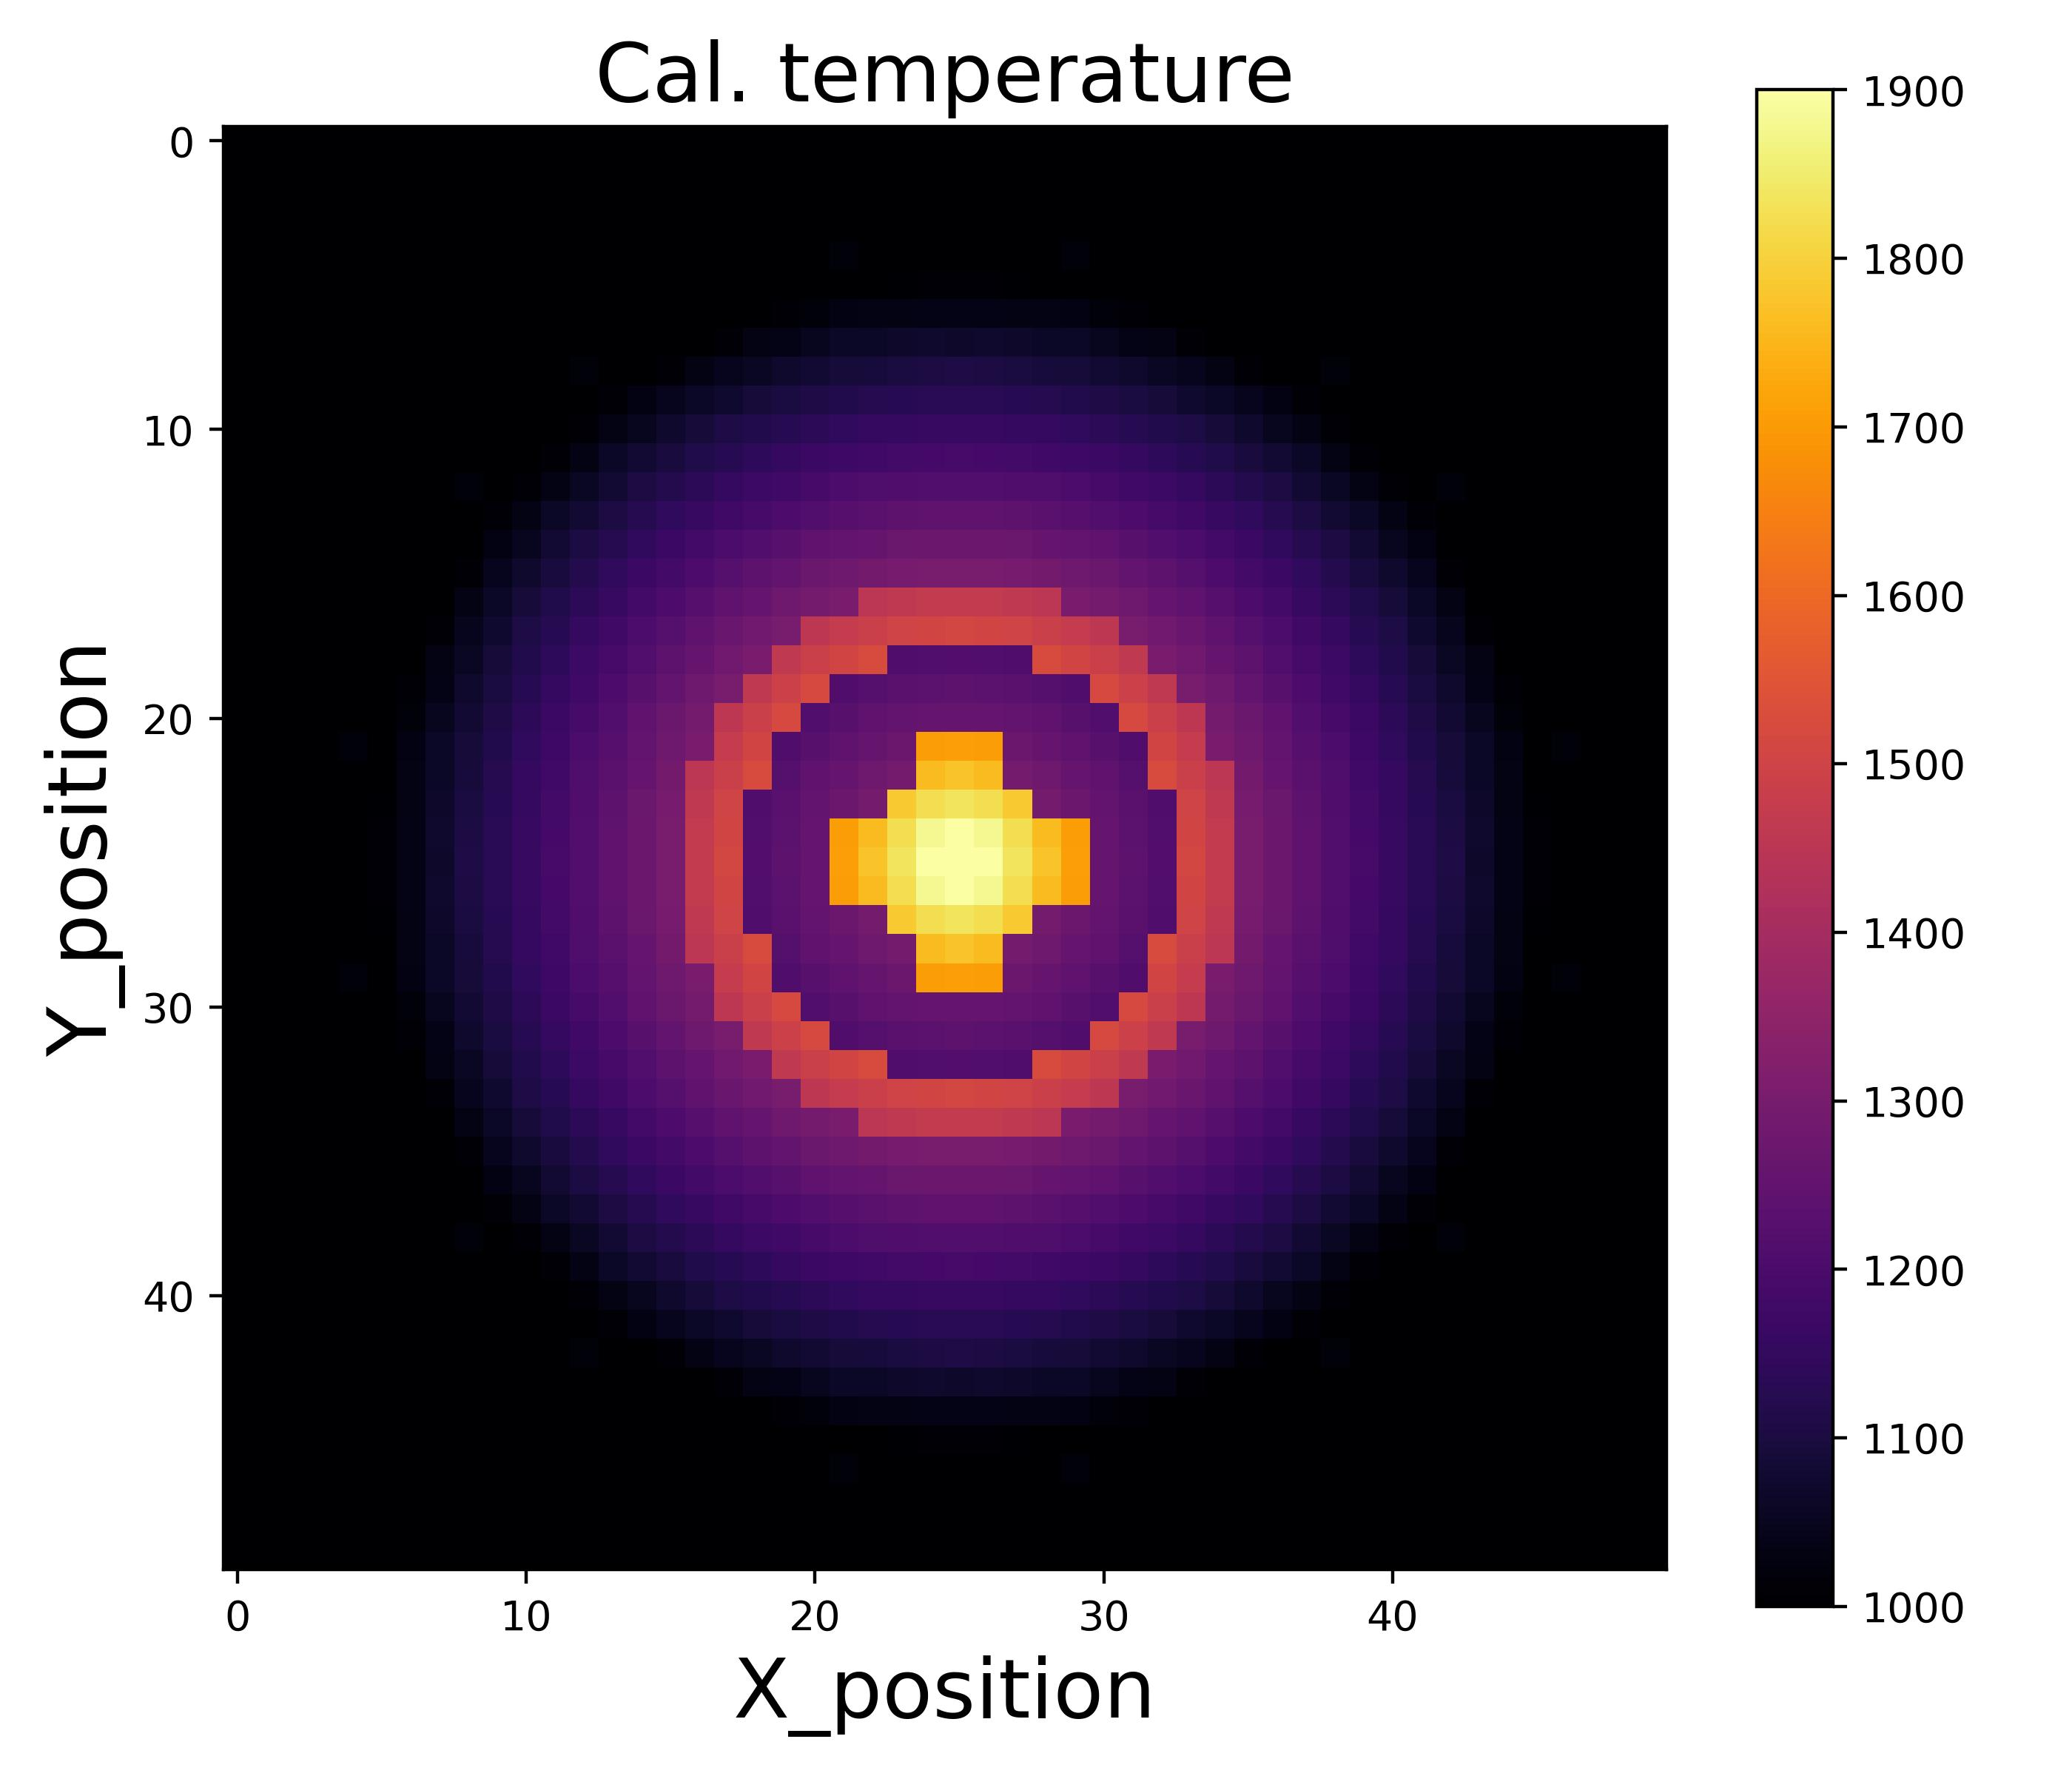
\includegraphics[width=\textwidth]{figures/raw_data/31/linear/T_cal.jpg}
            \subcaption{Model 7}
        \end{subfigure}
    \end{minipage}\\
    \begin{minipage}{\textwidth}
        \centering
        \begin{subfigure}{0.325\textwidth}
            \centering
            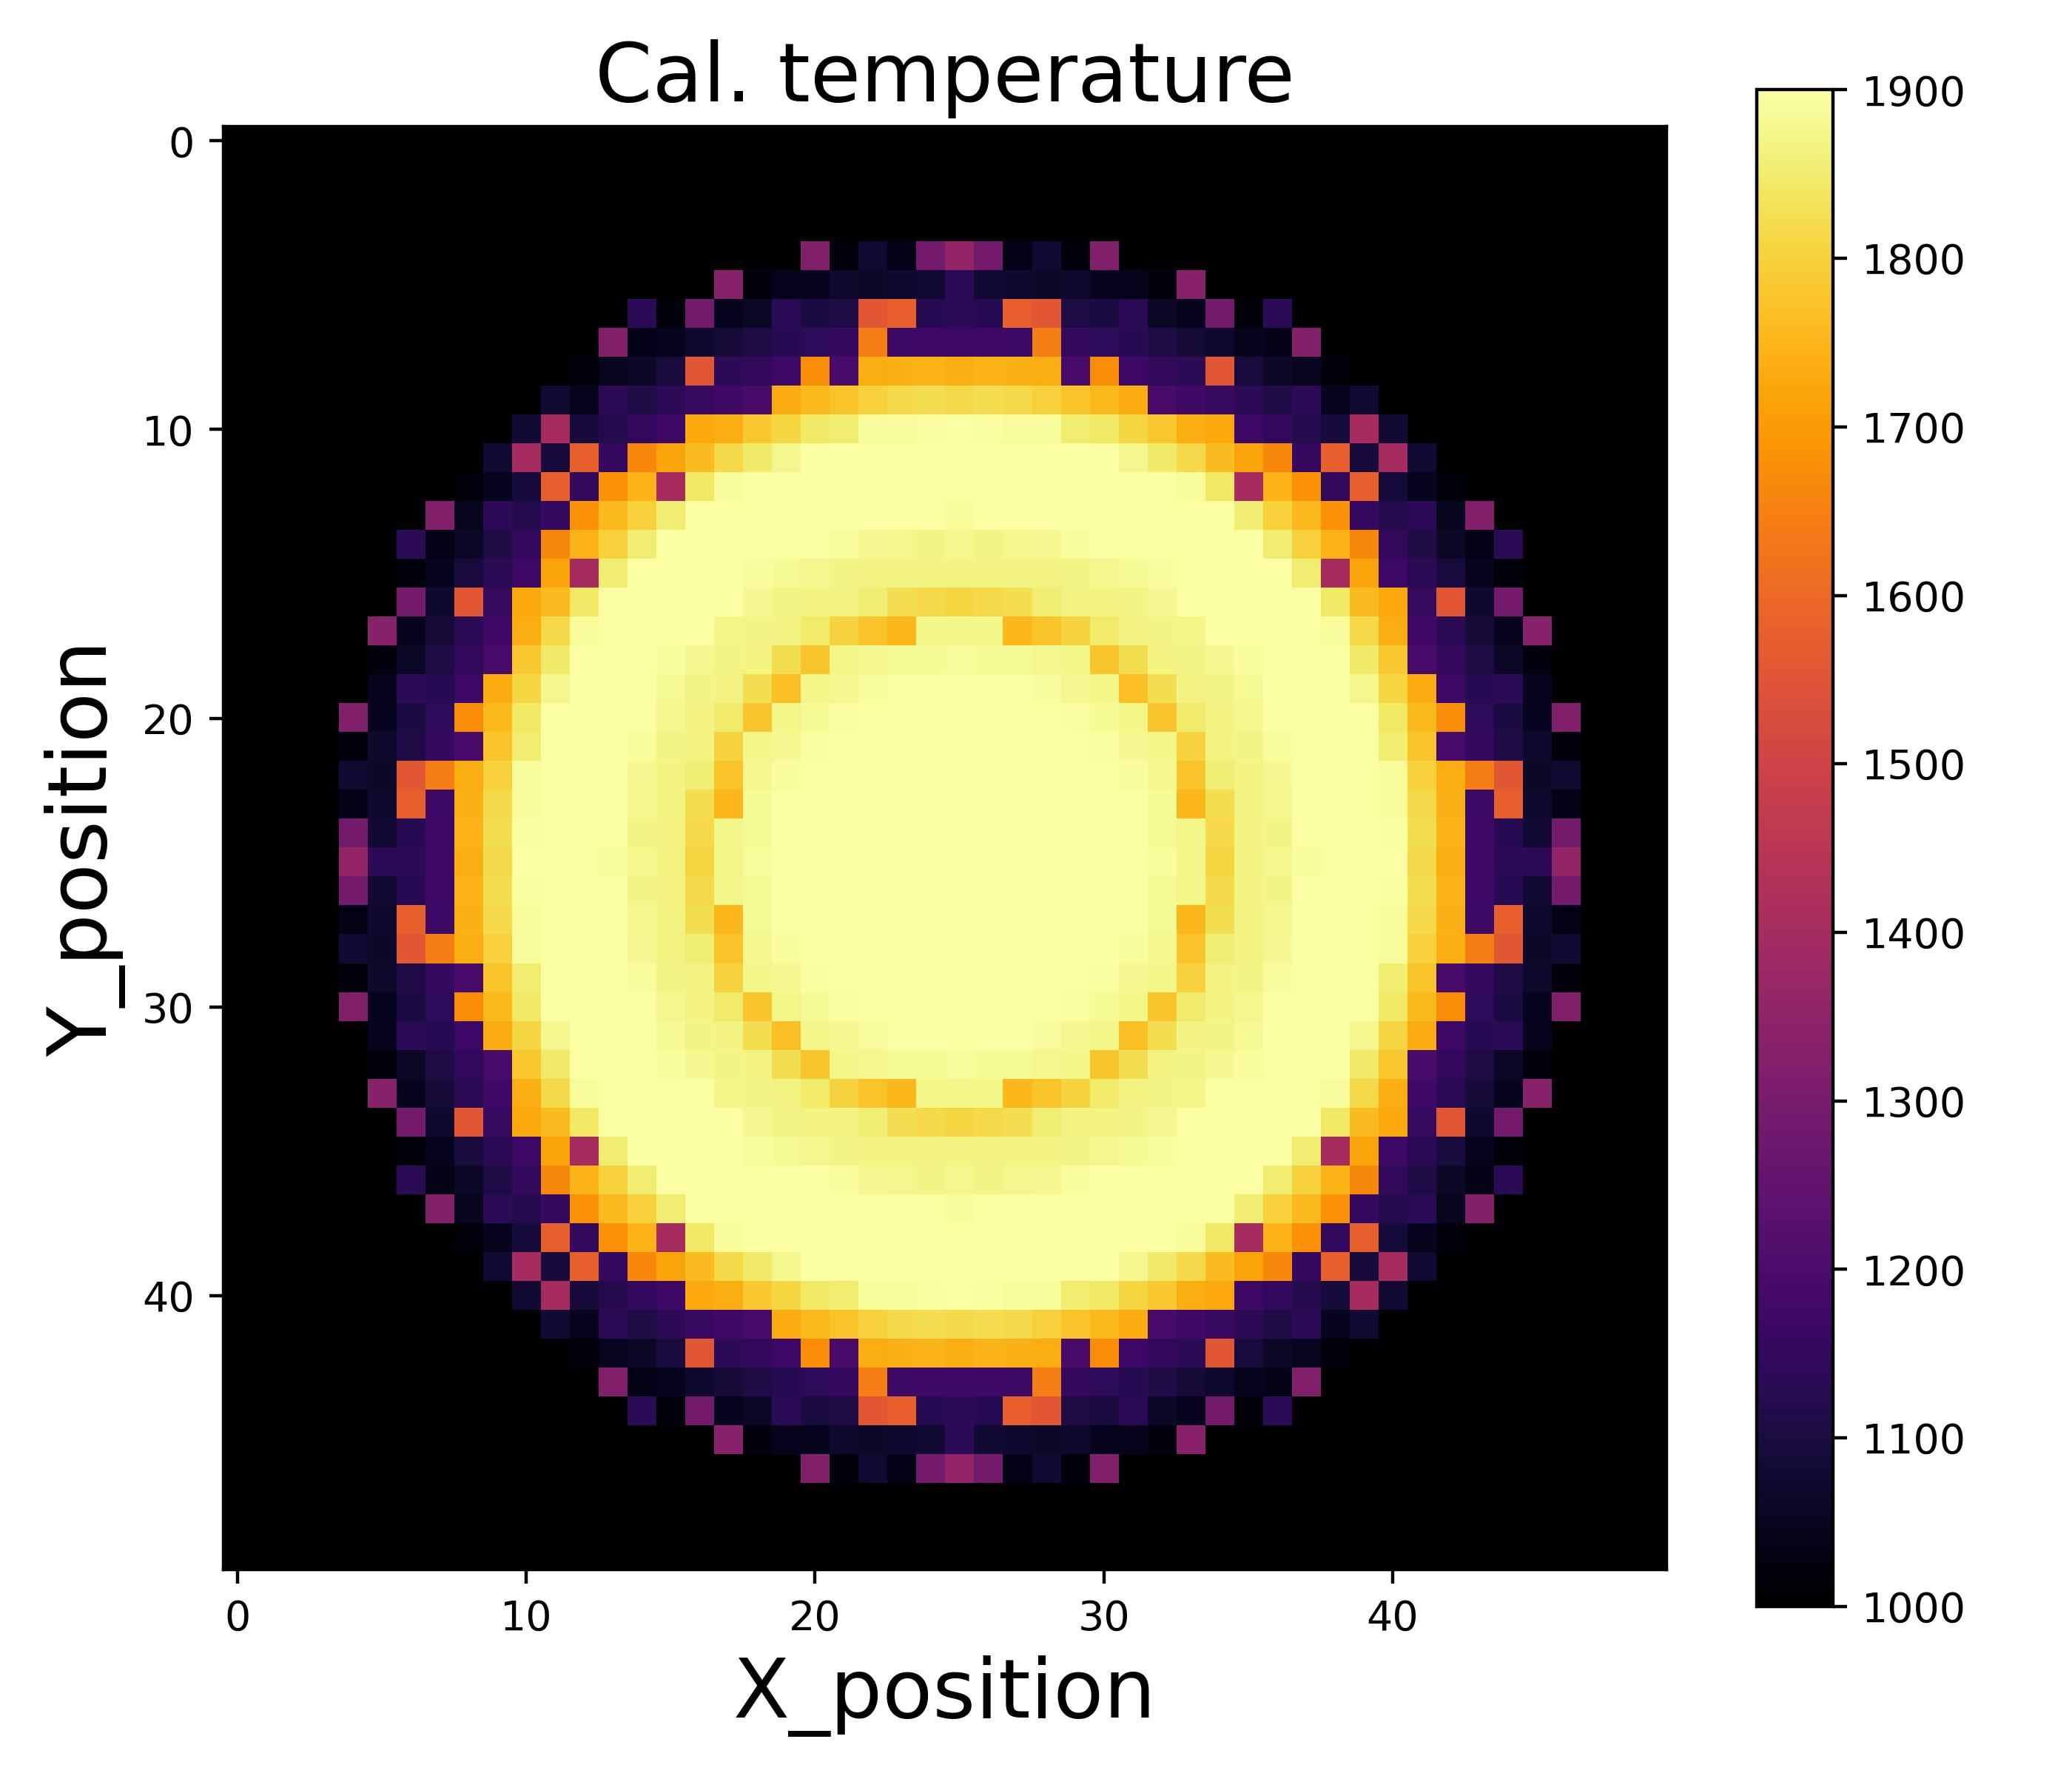
\includegraphics[width=\textwidth]{figures/raw_data/32/linear/T_cal.jpg}
            \subcaption{Model 8}
        \end{subfigure}
        \begin{subfigure}{0.325\textwidth}
            \centering
            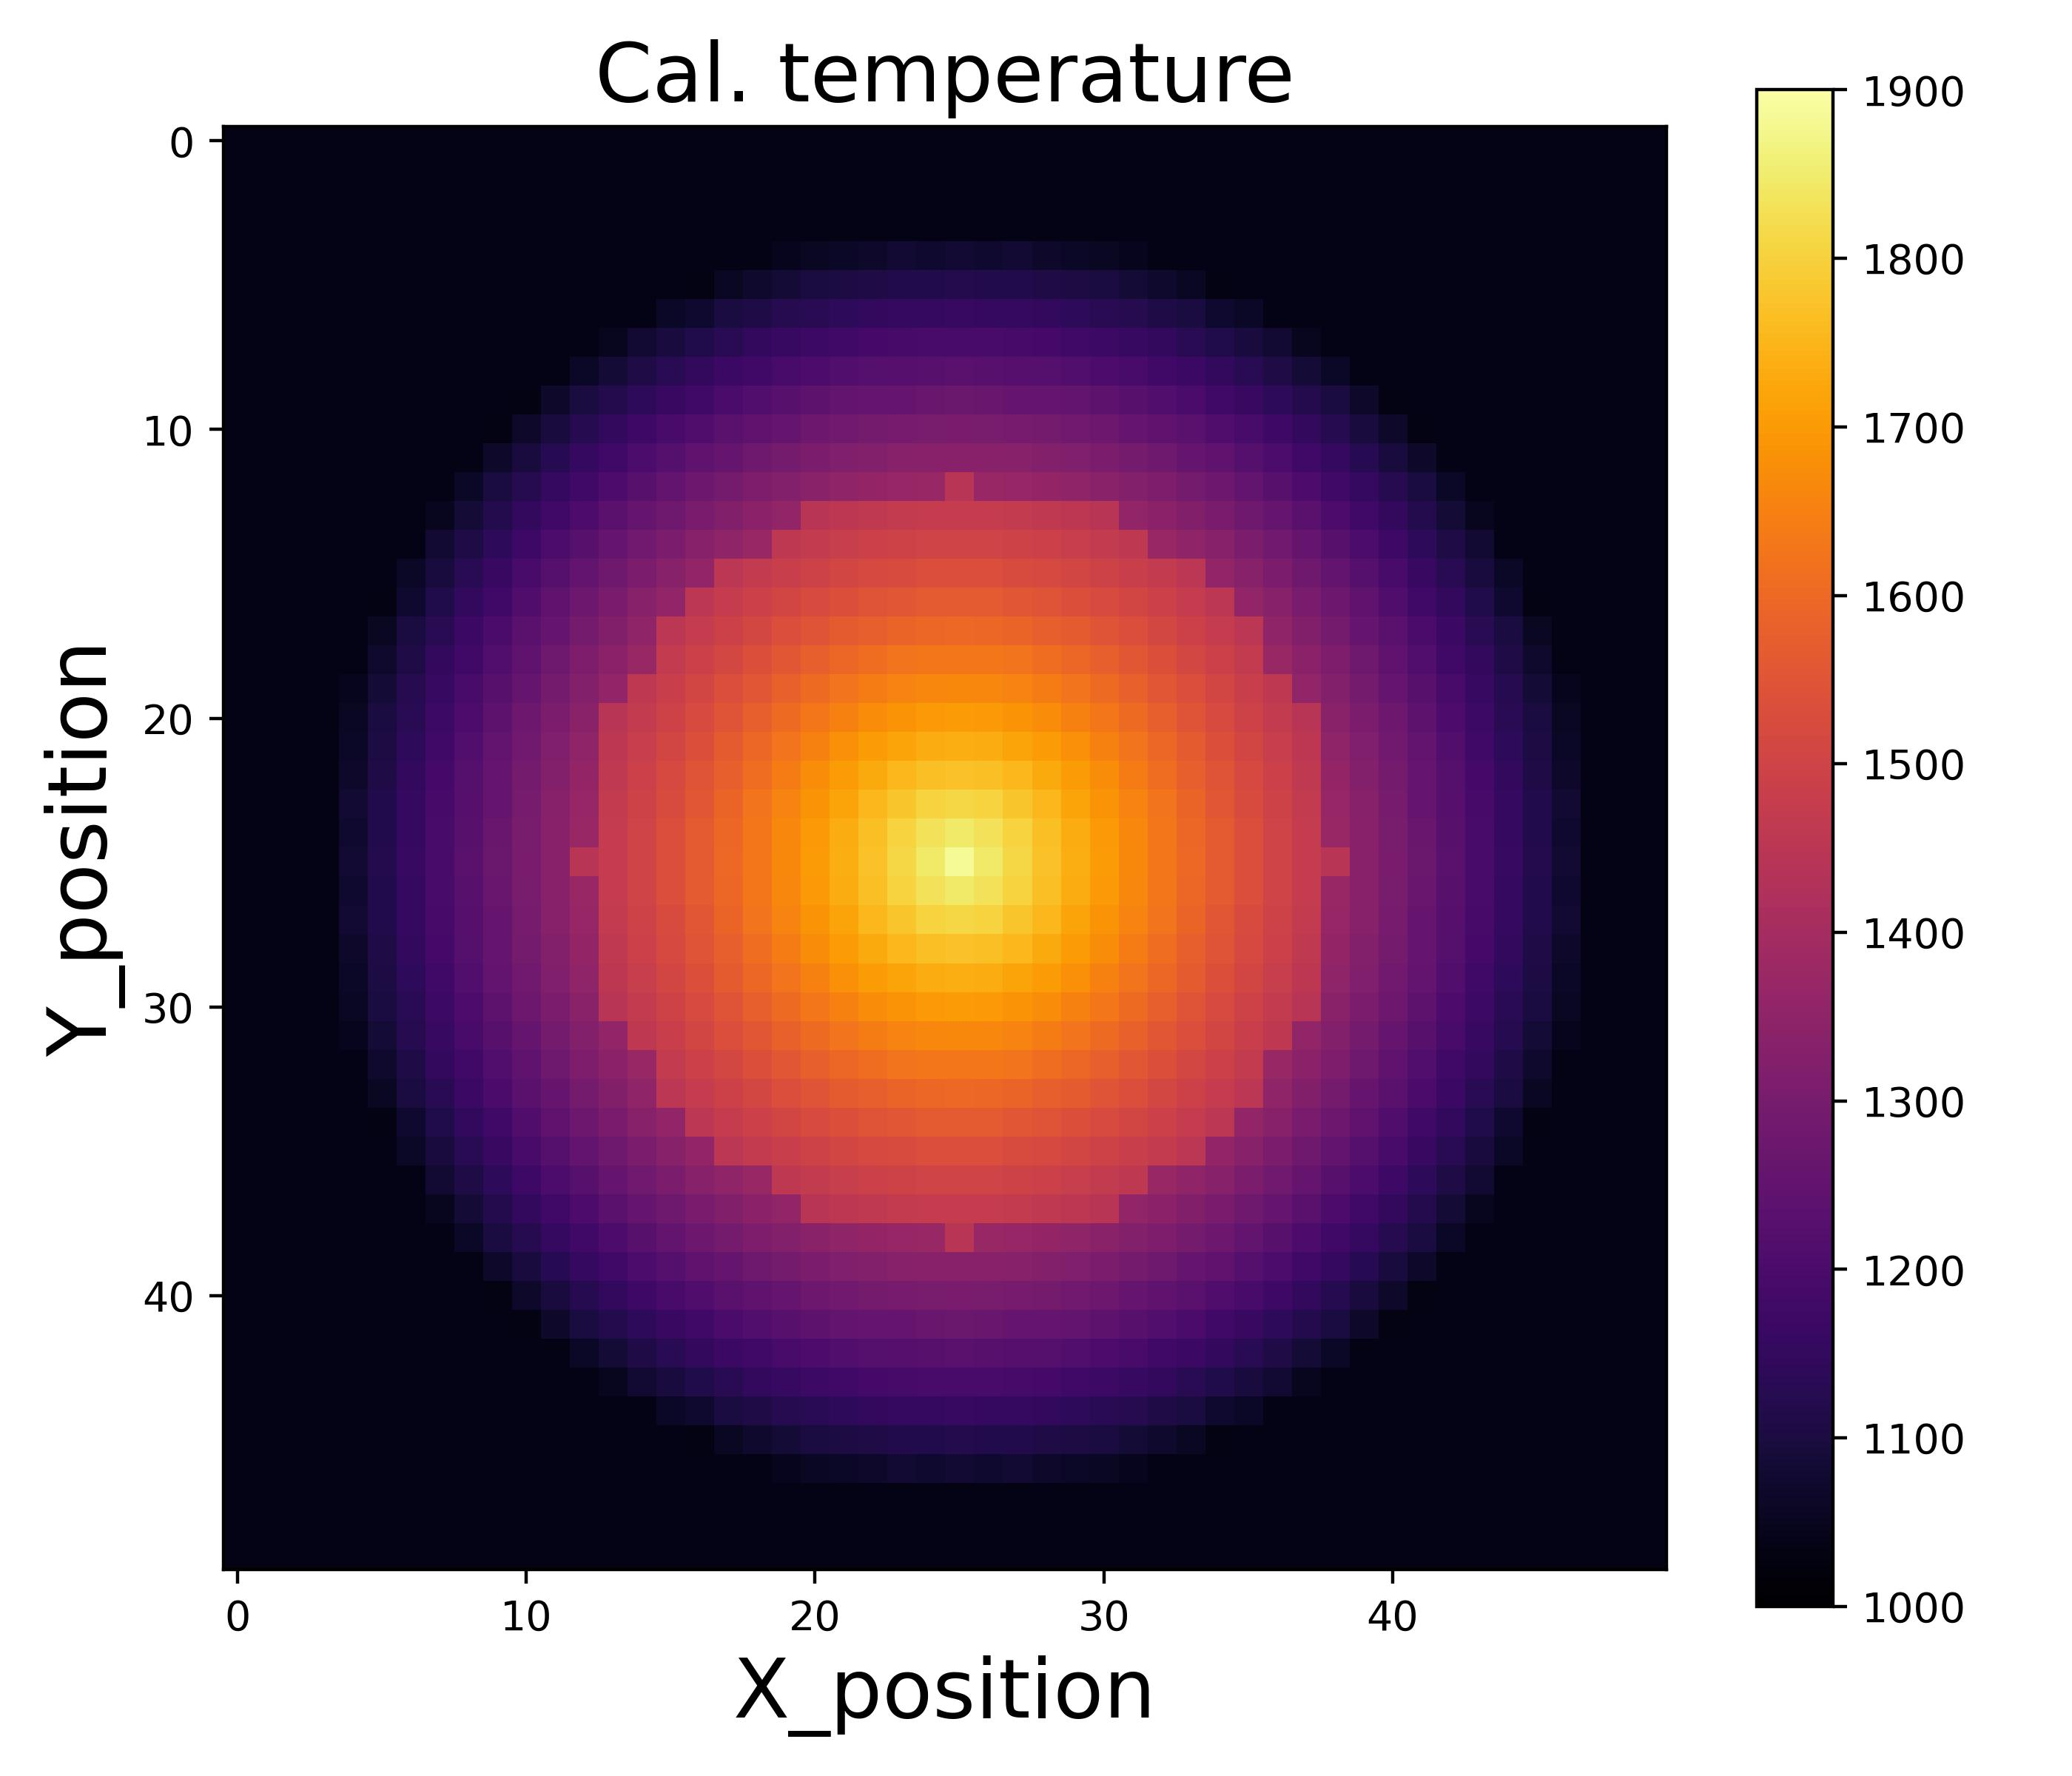
\includegraphics[width=\textwidth]{figures/raw_data/33/linear/T_cal.jpg}
            \subcaption{Model 9}
        \end{subfigure}
    \end{minipage}
    \caption{Temperature calculation results of linear model}  
\end{figure}
\begin{figure}[p]
    \centering
    \begin{minipage}{\textwidth}
        \centering
        \begin{subfigure}{0.325\textwidth}
            \centering
            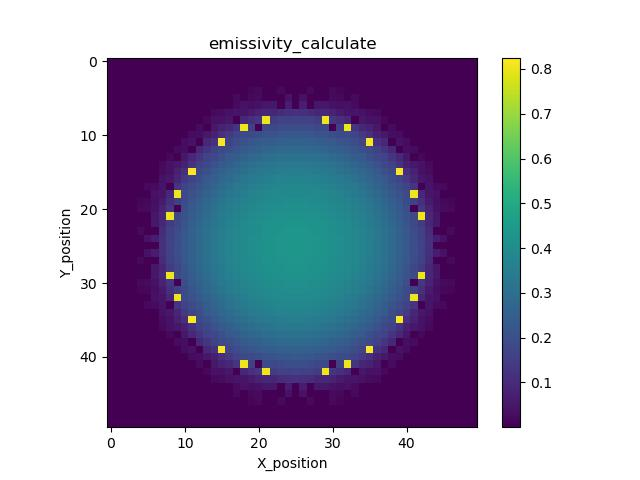
\includegraphics[width=\textwidth]{figures/raw_data/0/linear/emi_cal.jpg}
            \subcaption{Black body material}
        \end{subfigure}
        \begin{subfigure}{0.325\textwidth}
            \centering
            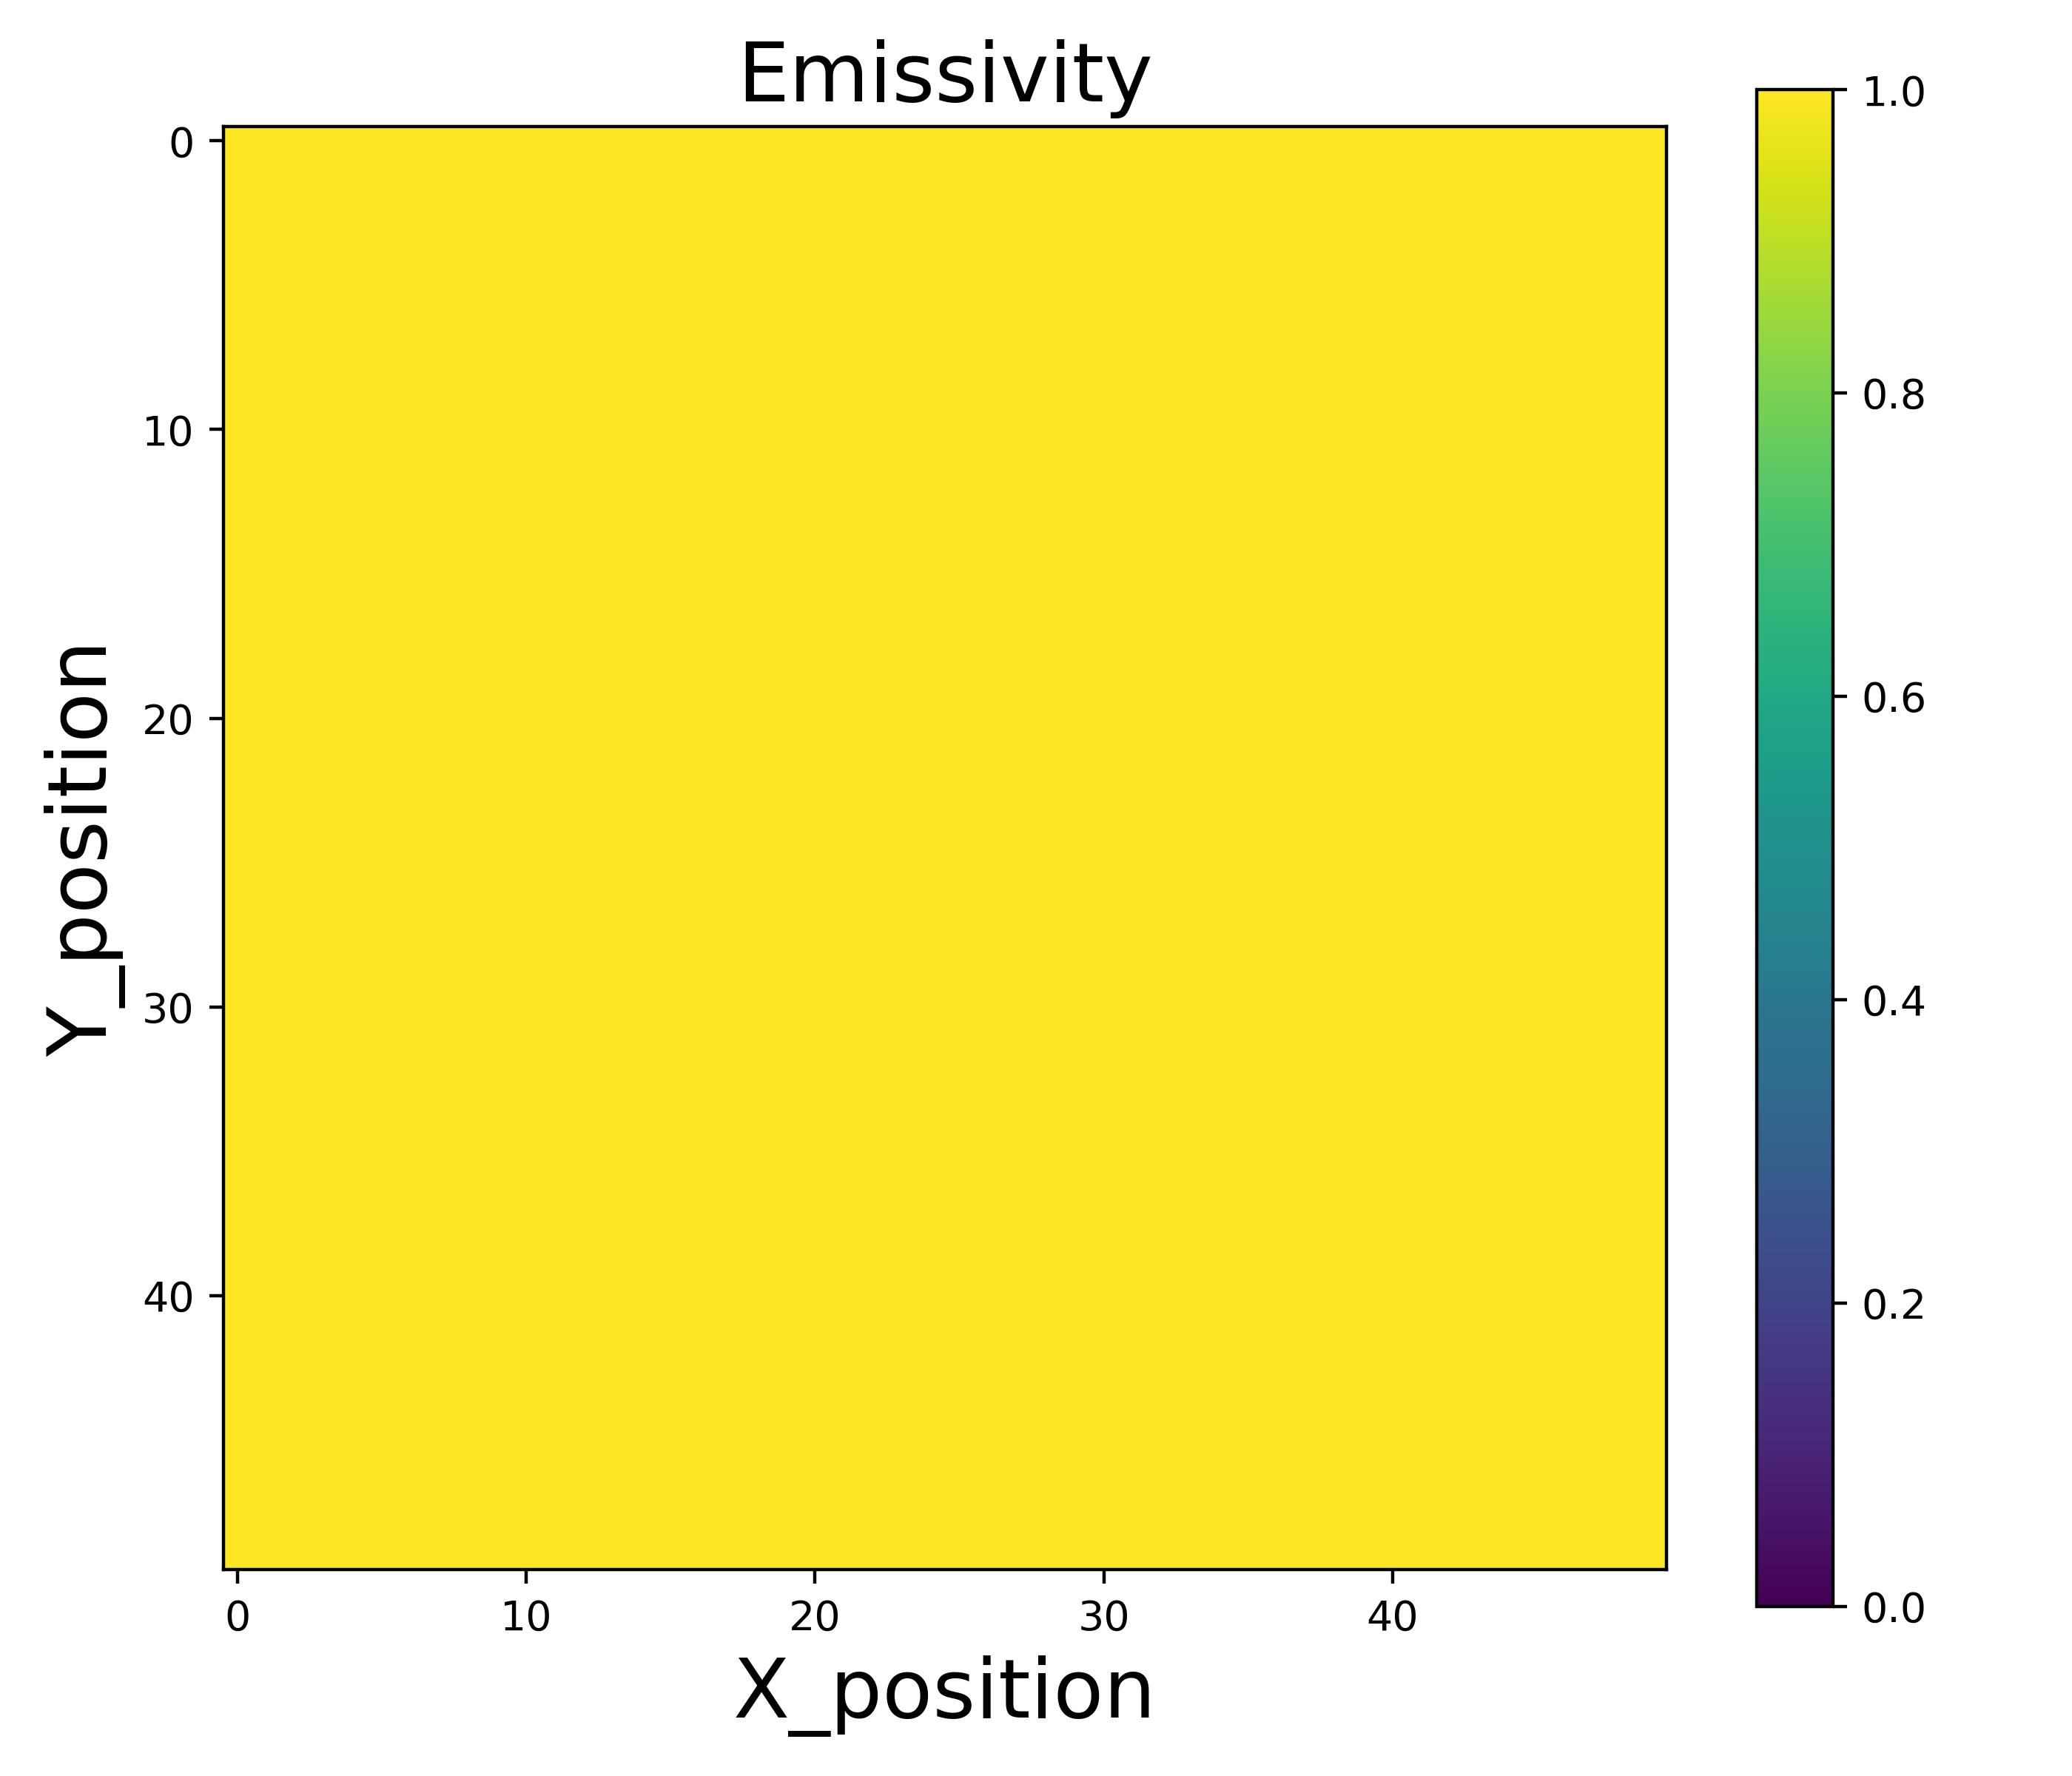
\includegraphics[width=\textwidth]{figures/raw_data/5/linear/emi_cal.jpg}
            \subcaption{Real iron data}
        \end{subfigure}
        \begin{subfigure}{0.325\textwidth}
            \centering
            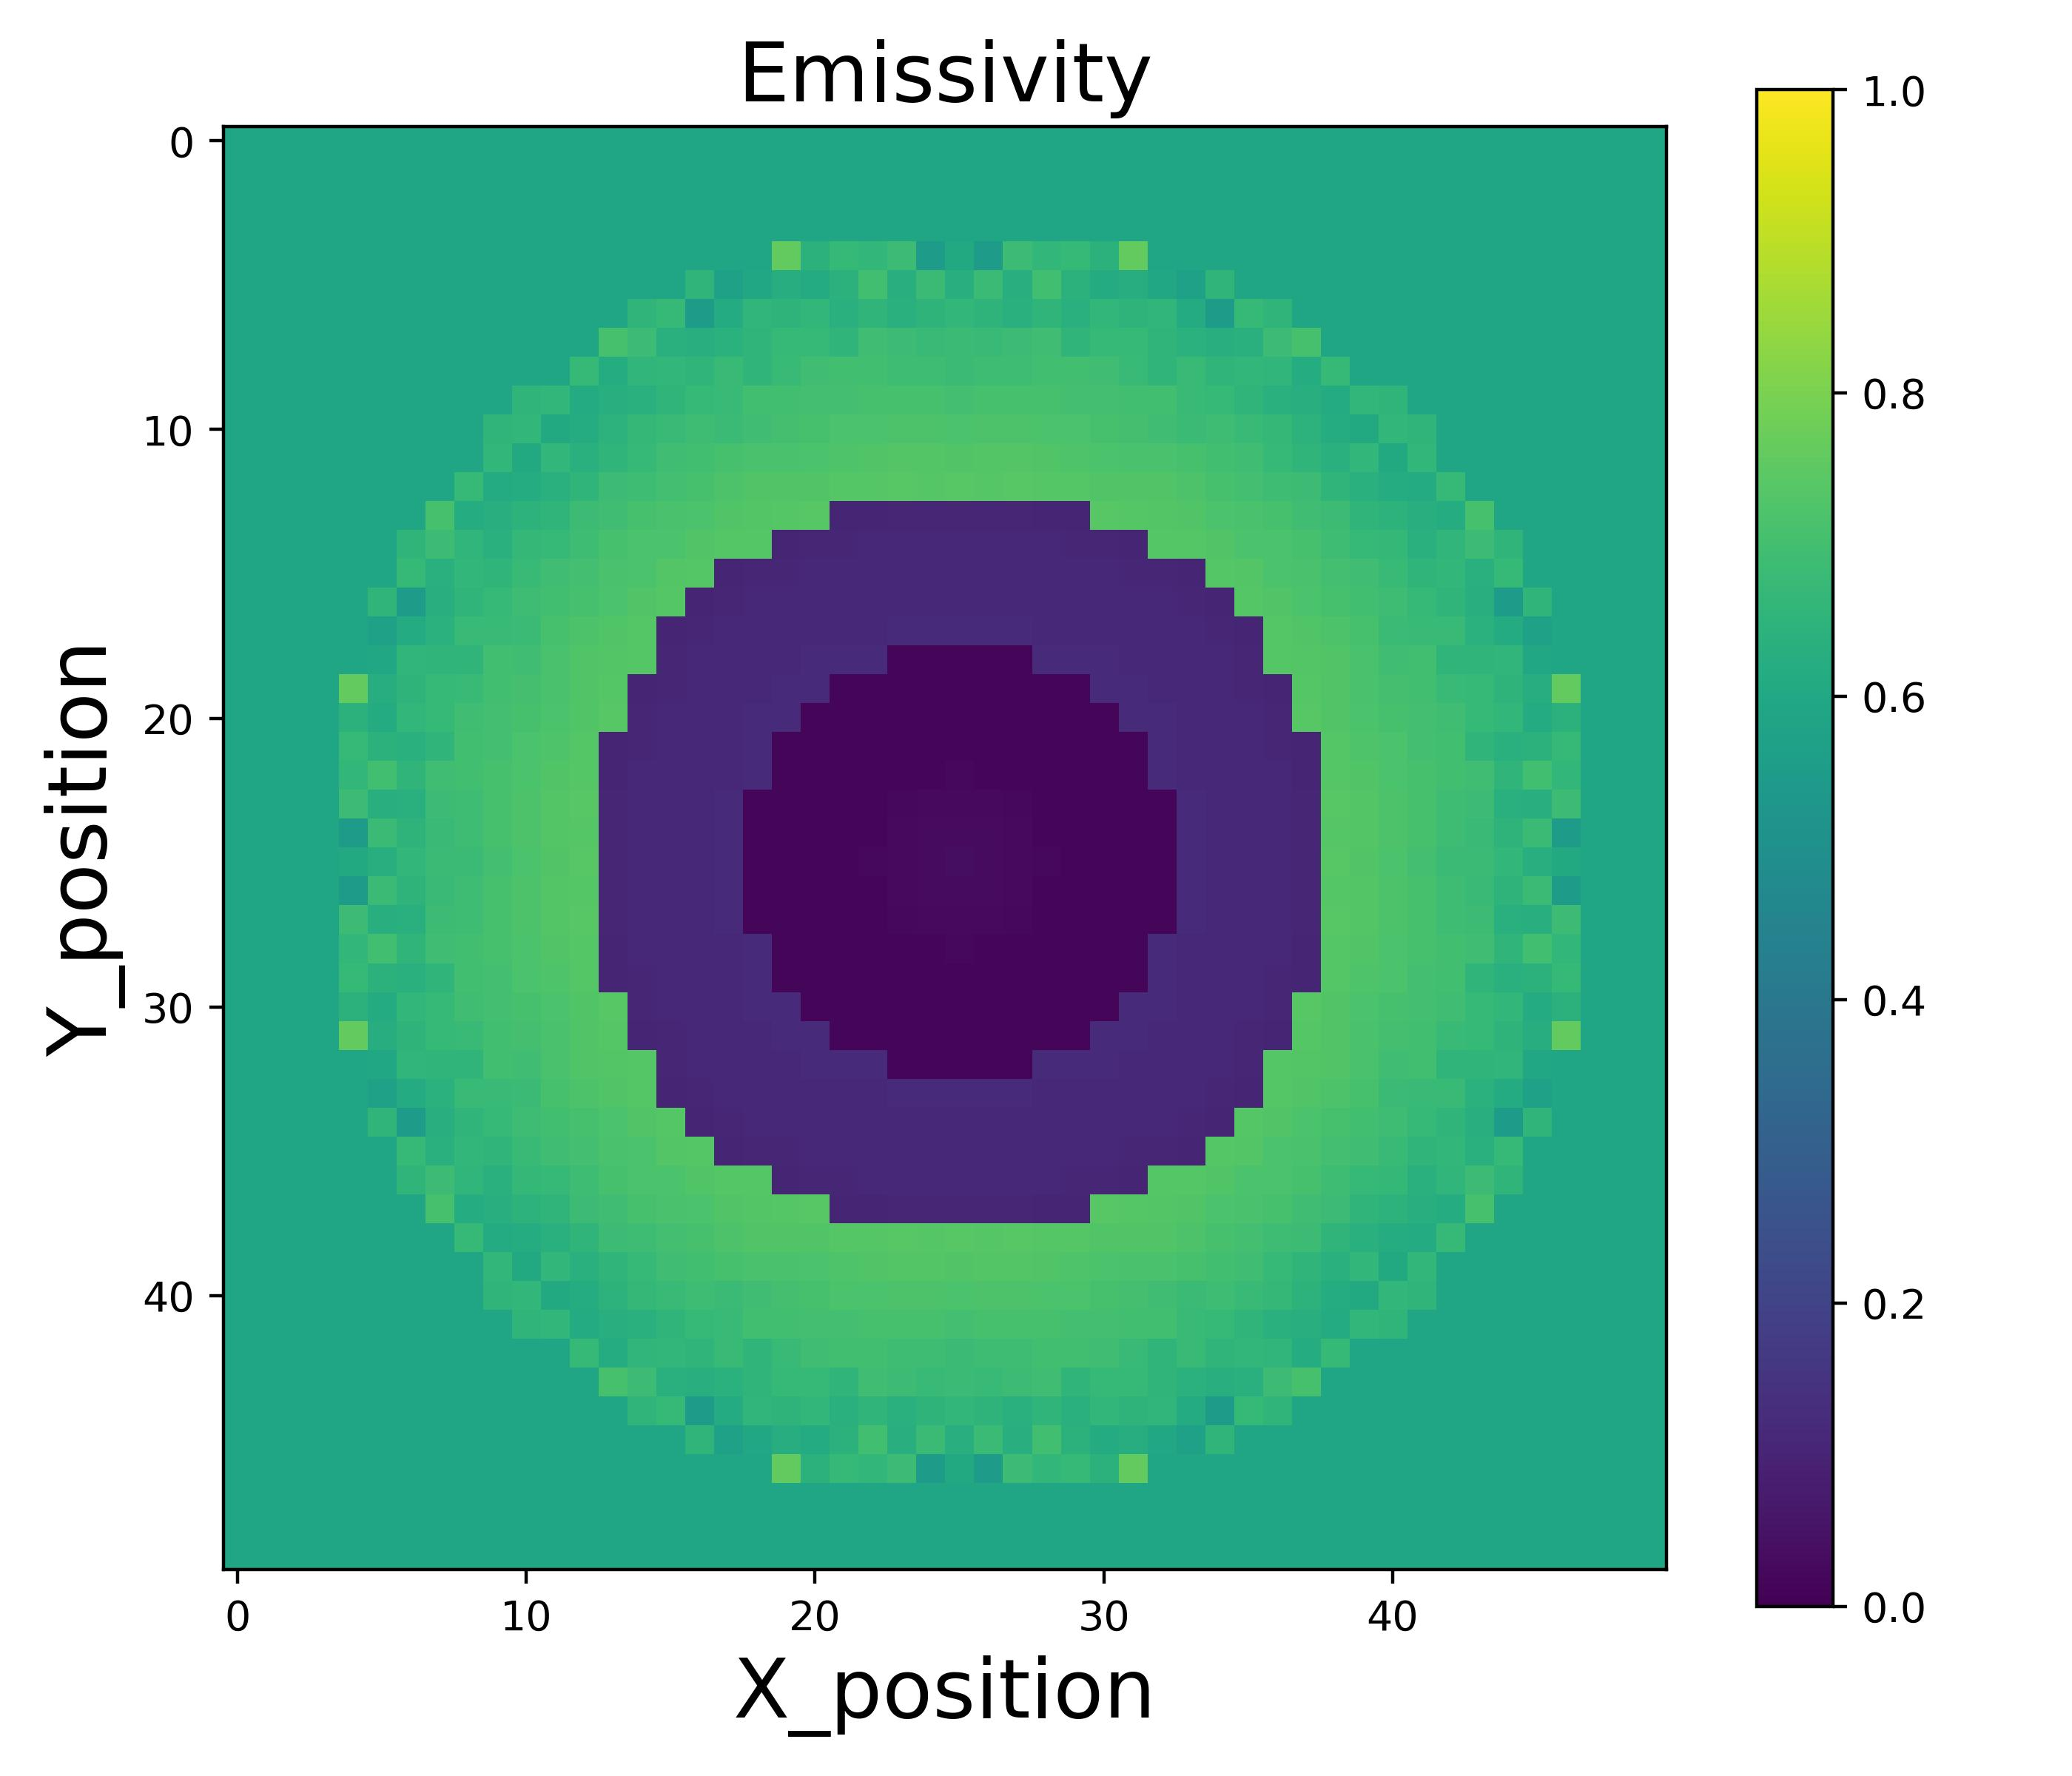
\includegraphics[width=\textwidth]{figures/raw_data/21/linear/emi_cal.jpg}
            \subcaption{Model 1}
        \end{subfigure}
    \end{minipage}\\
    \begin{minipage}{\textwidth}
        \centering
        \begin{subfigure}{0.325\textwidth}
            \centering
            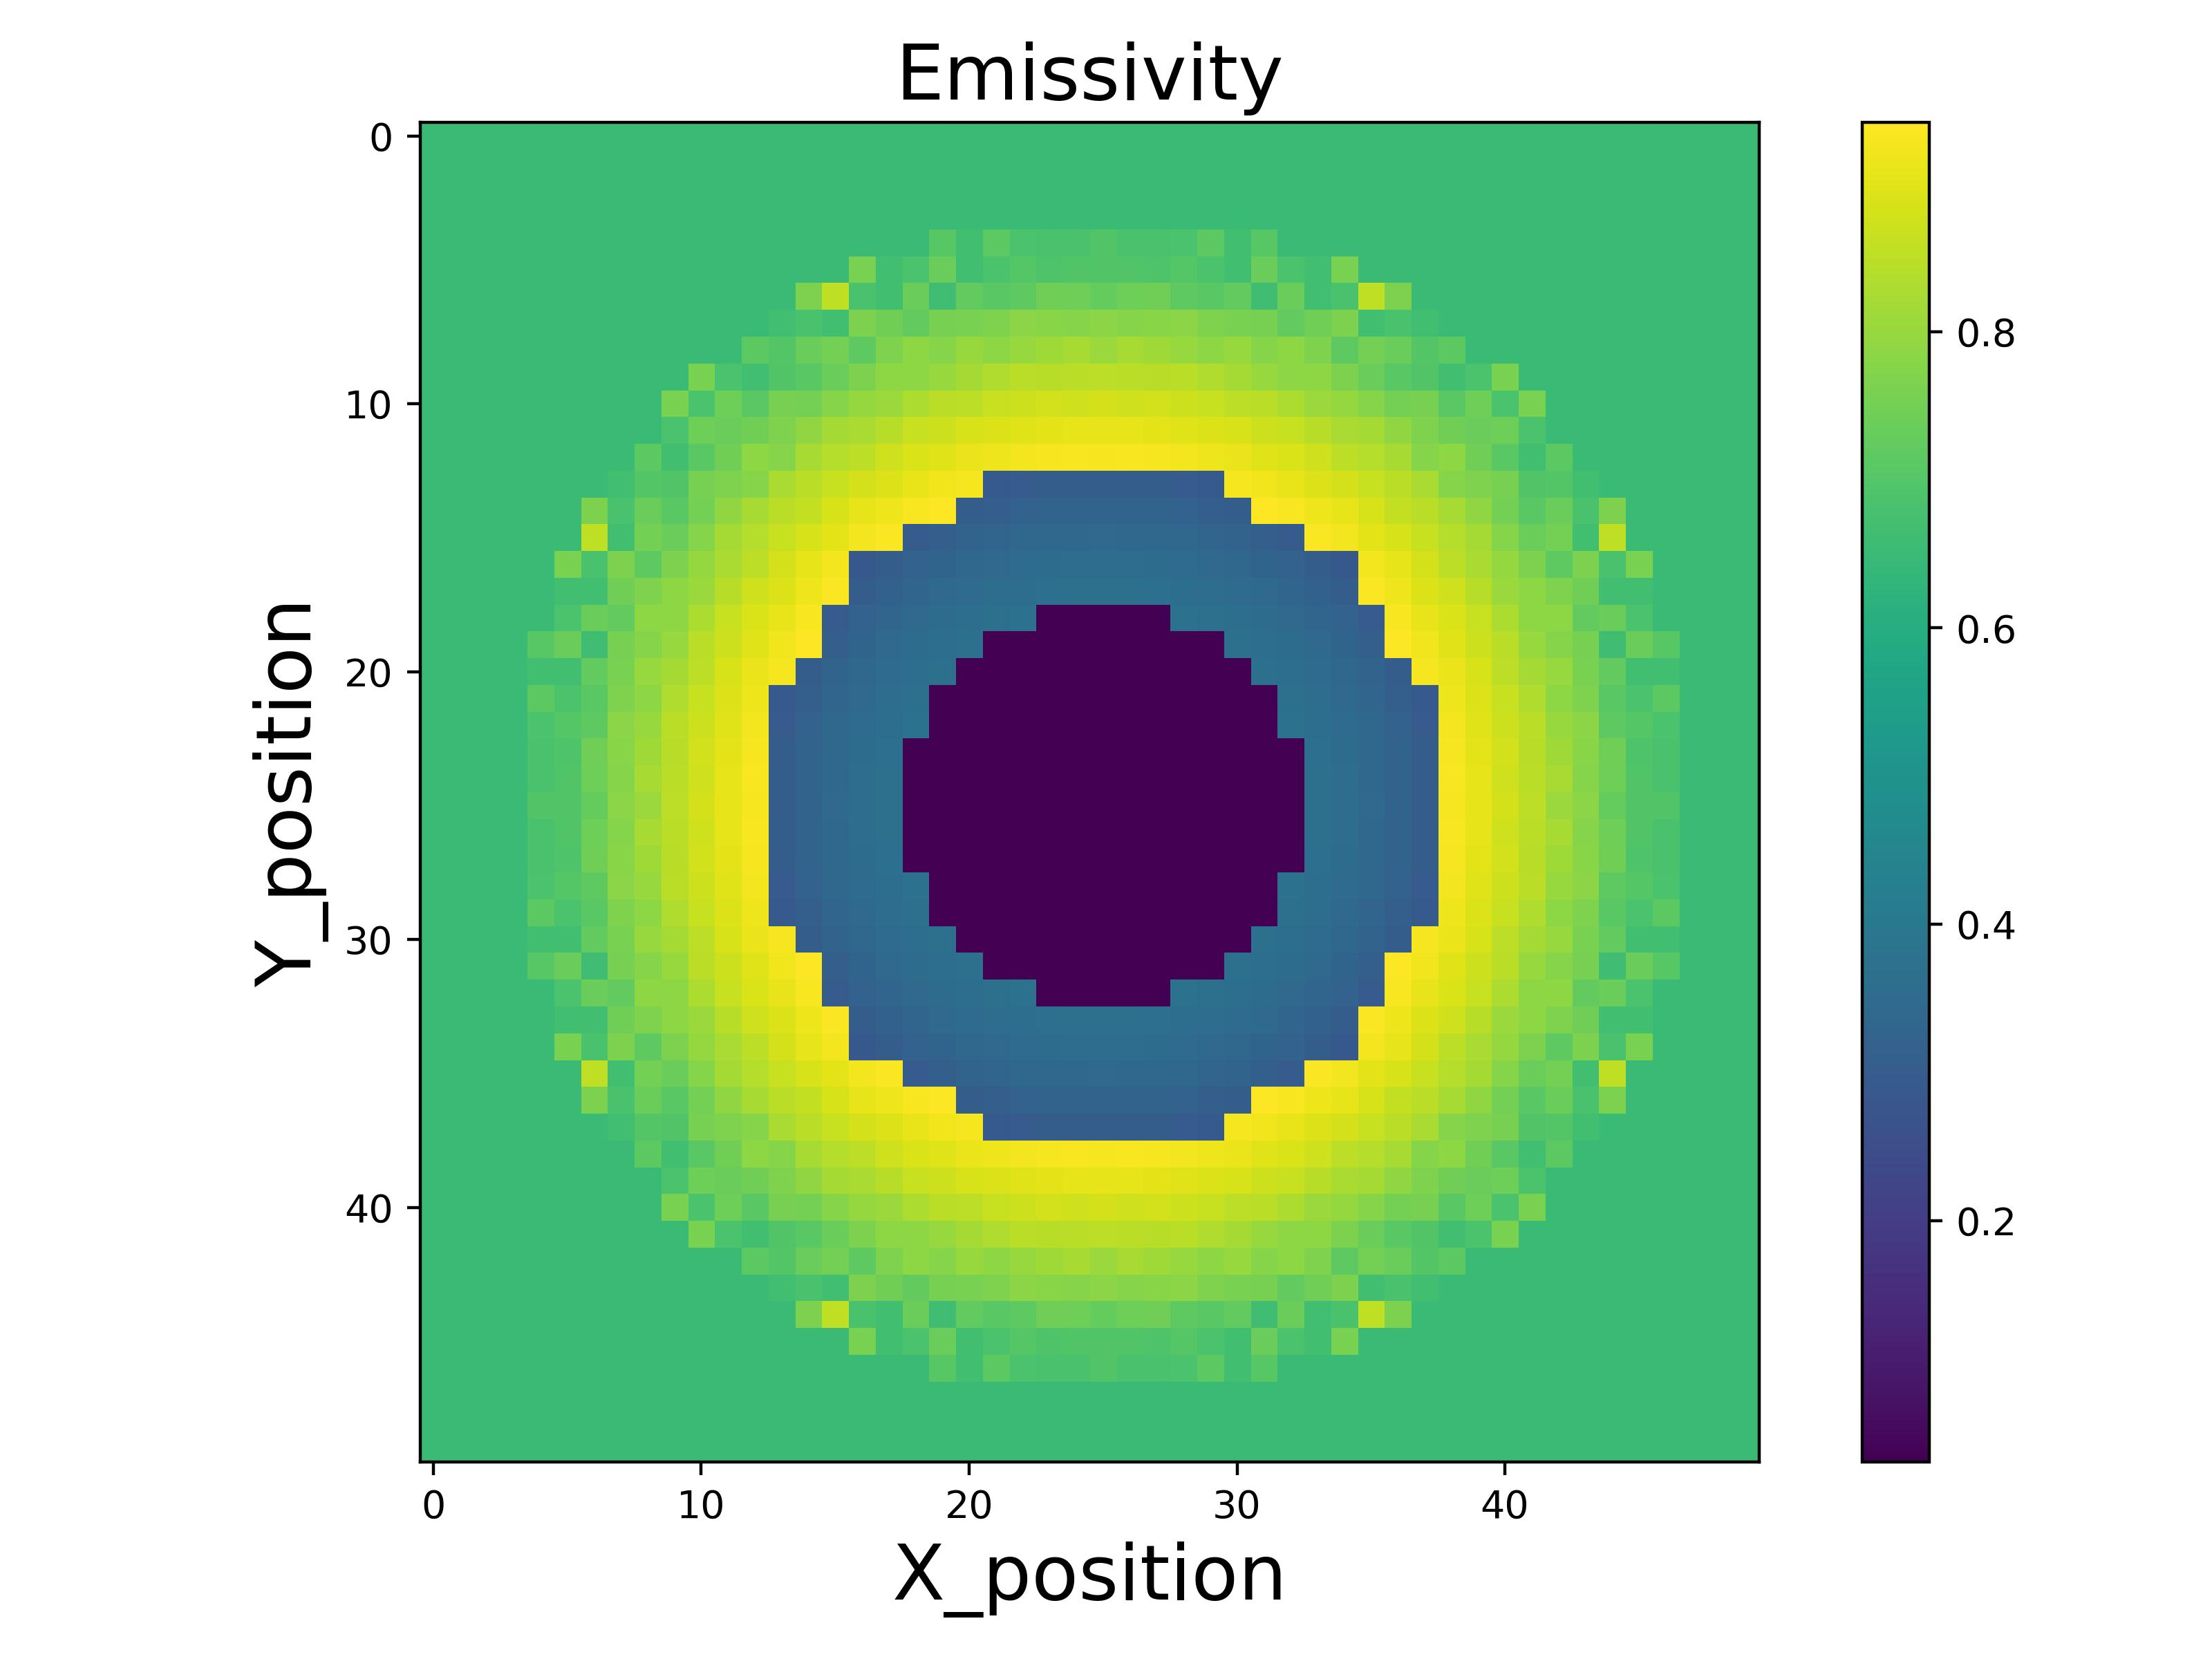
\includegraphics[width=\textwidth]{figures/raw_data/22/linear/emi_cal.jpg}
            \subcaption{Model 2}
        \end{subfigure}
        \begin{subfigure}{0.325\textwidth}
            \centering
            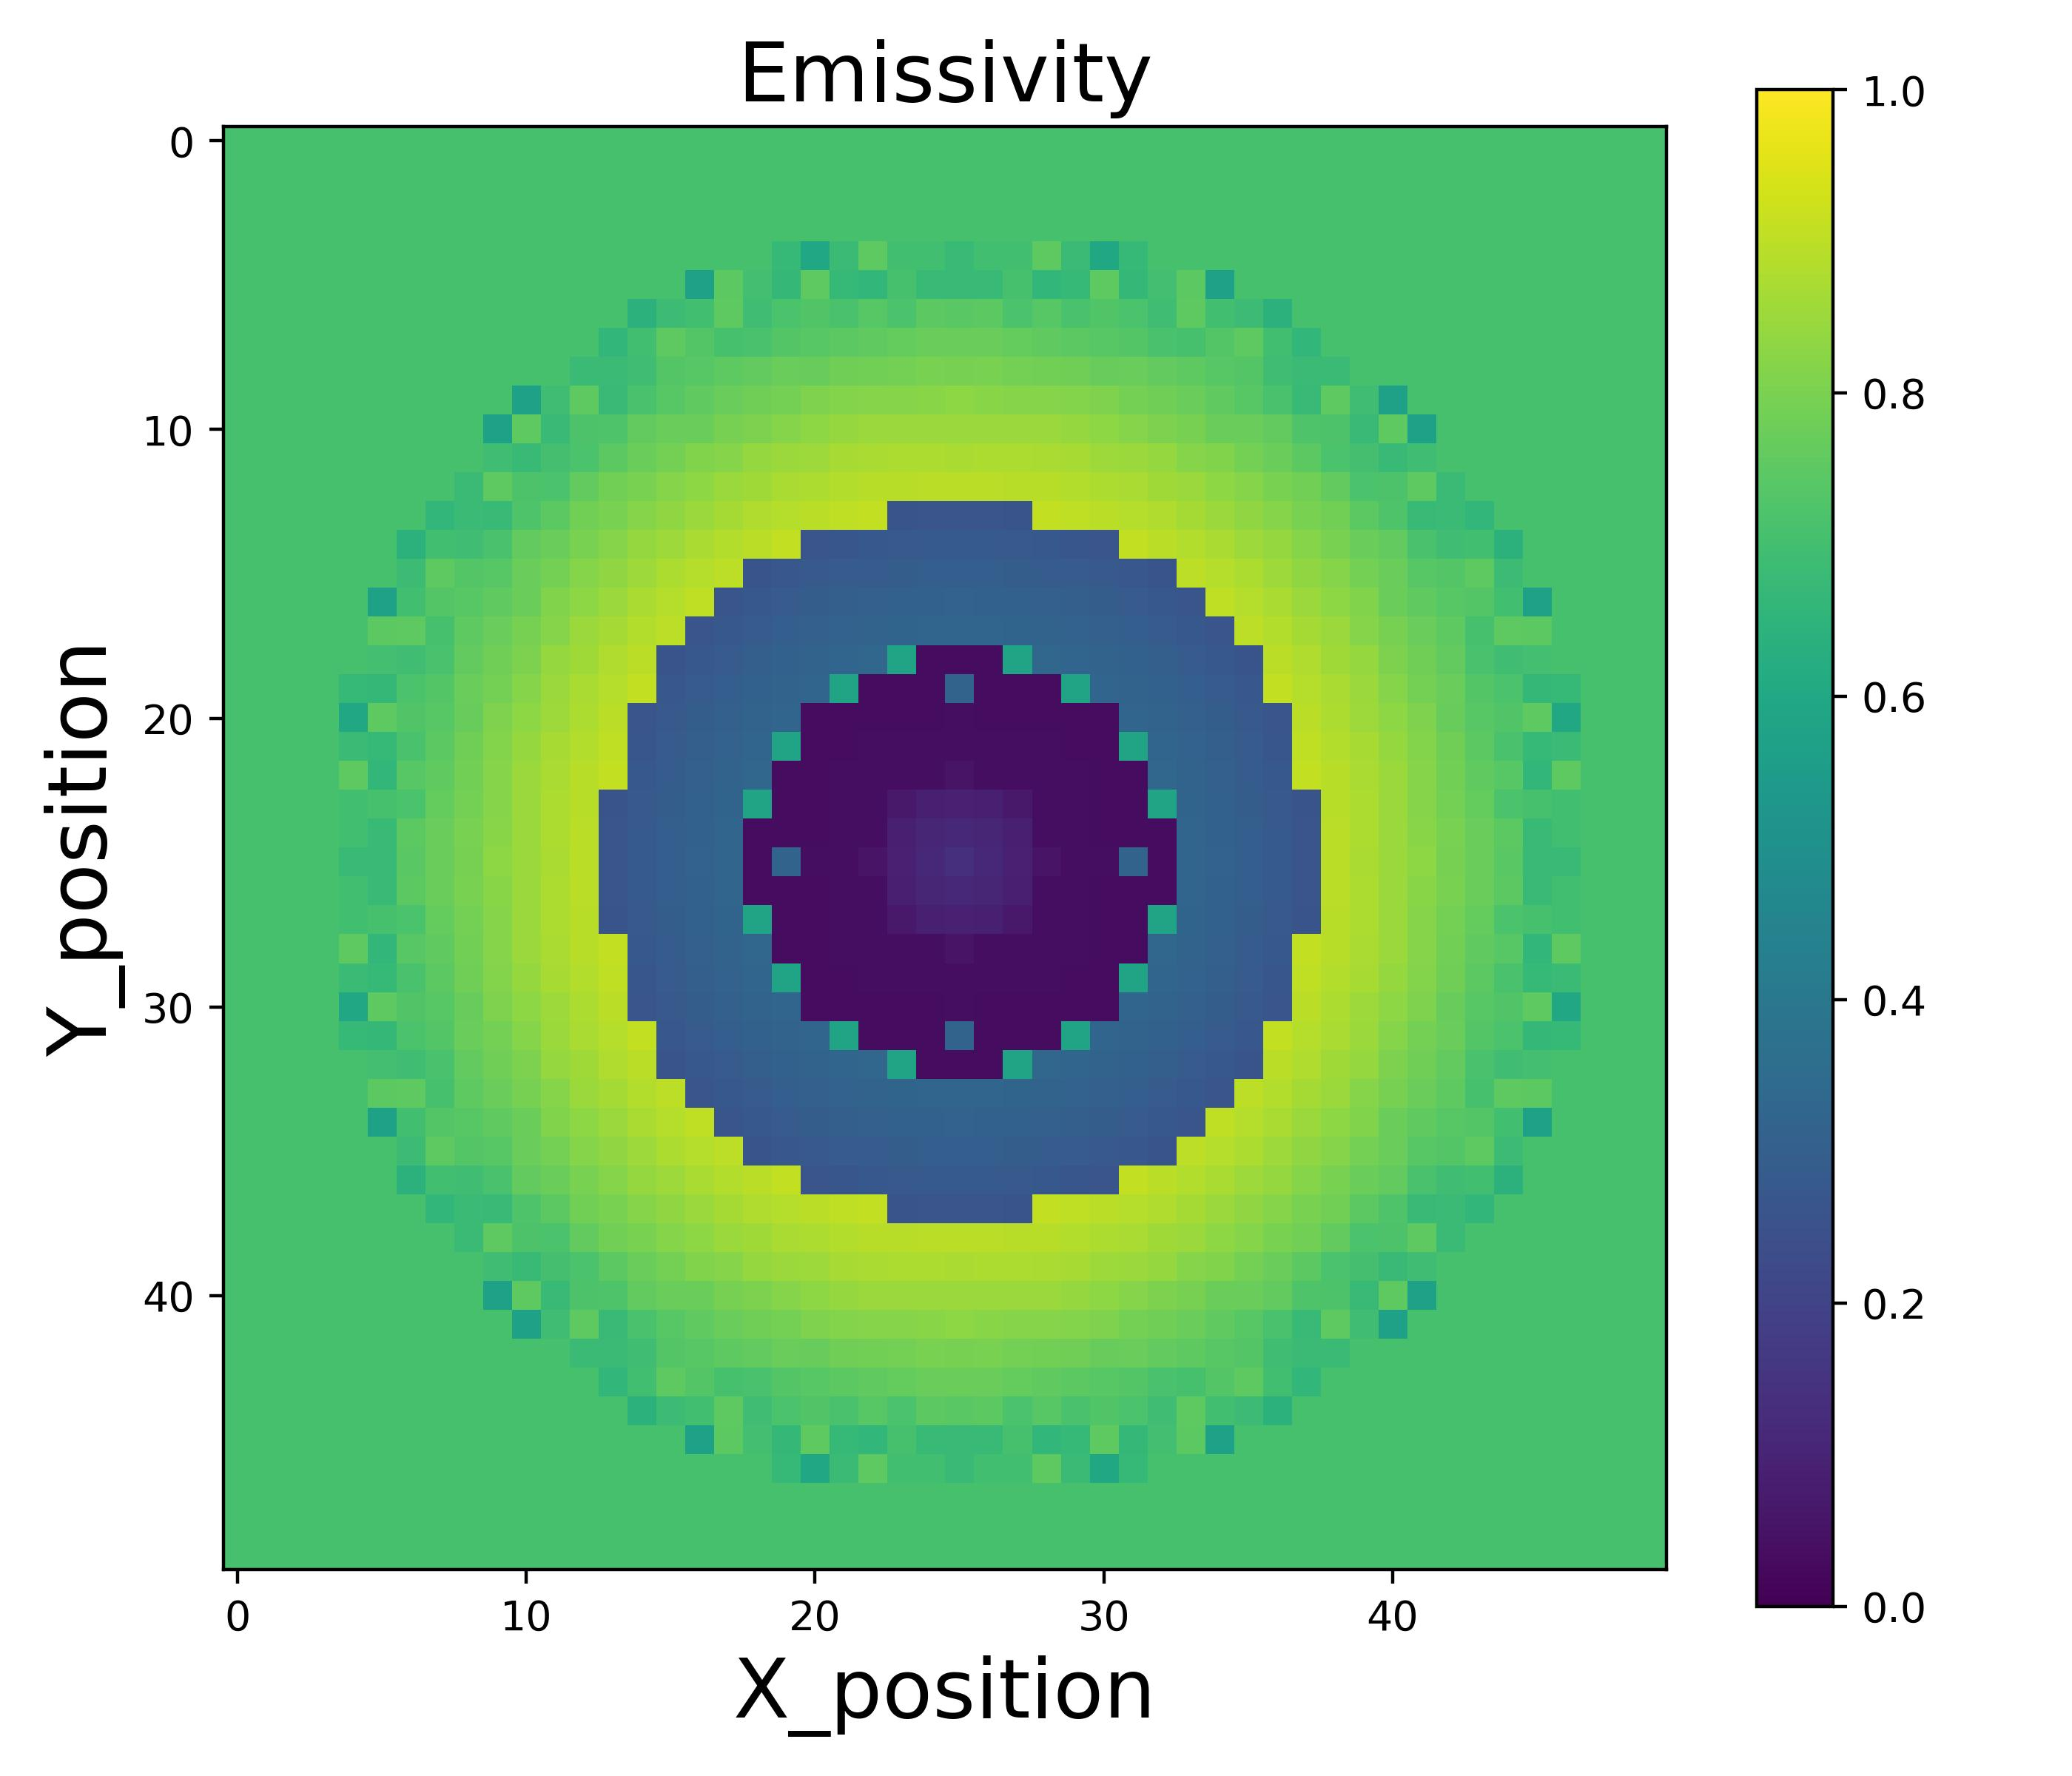
\includegraphics[width=\textwidth]{figures/raw_data/23/linear/emi_cal.jpg}
            \subcaption{Model 3}
        \end{subfigure}
        \begin{subfigure}{0.325\textwidth}
            \centering
            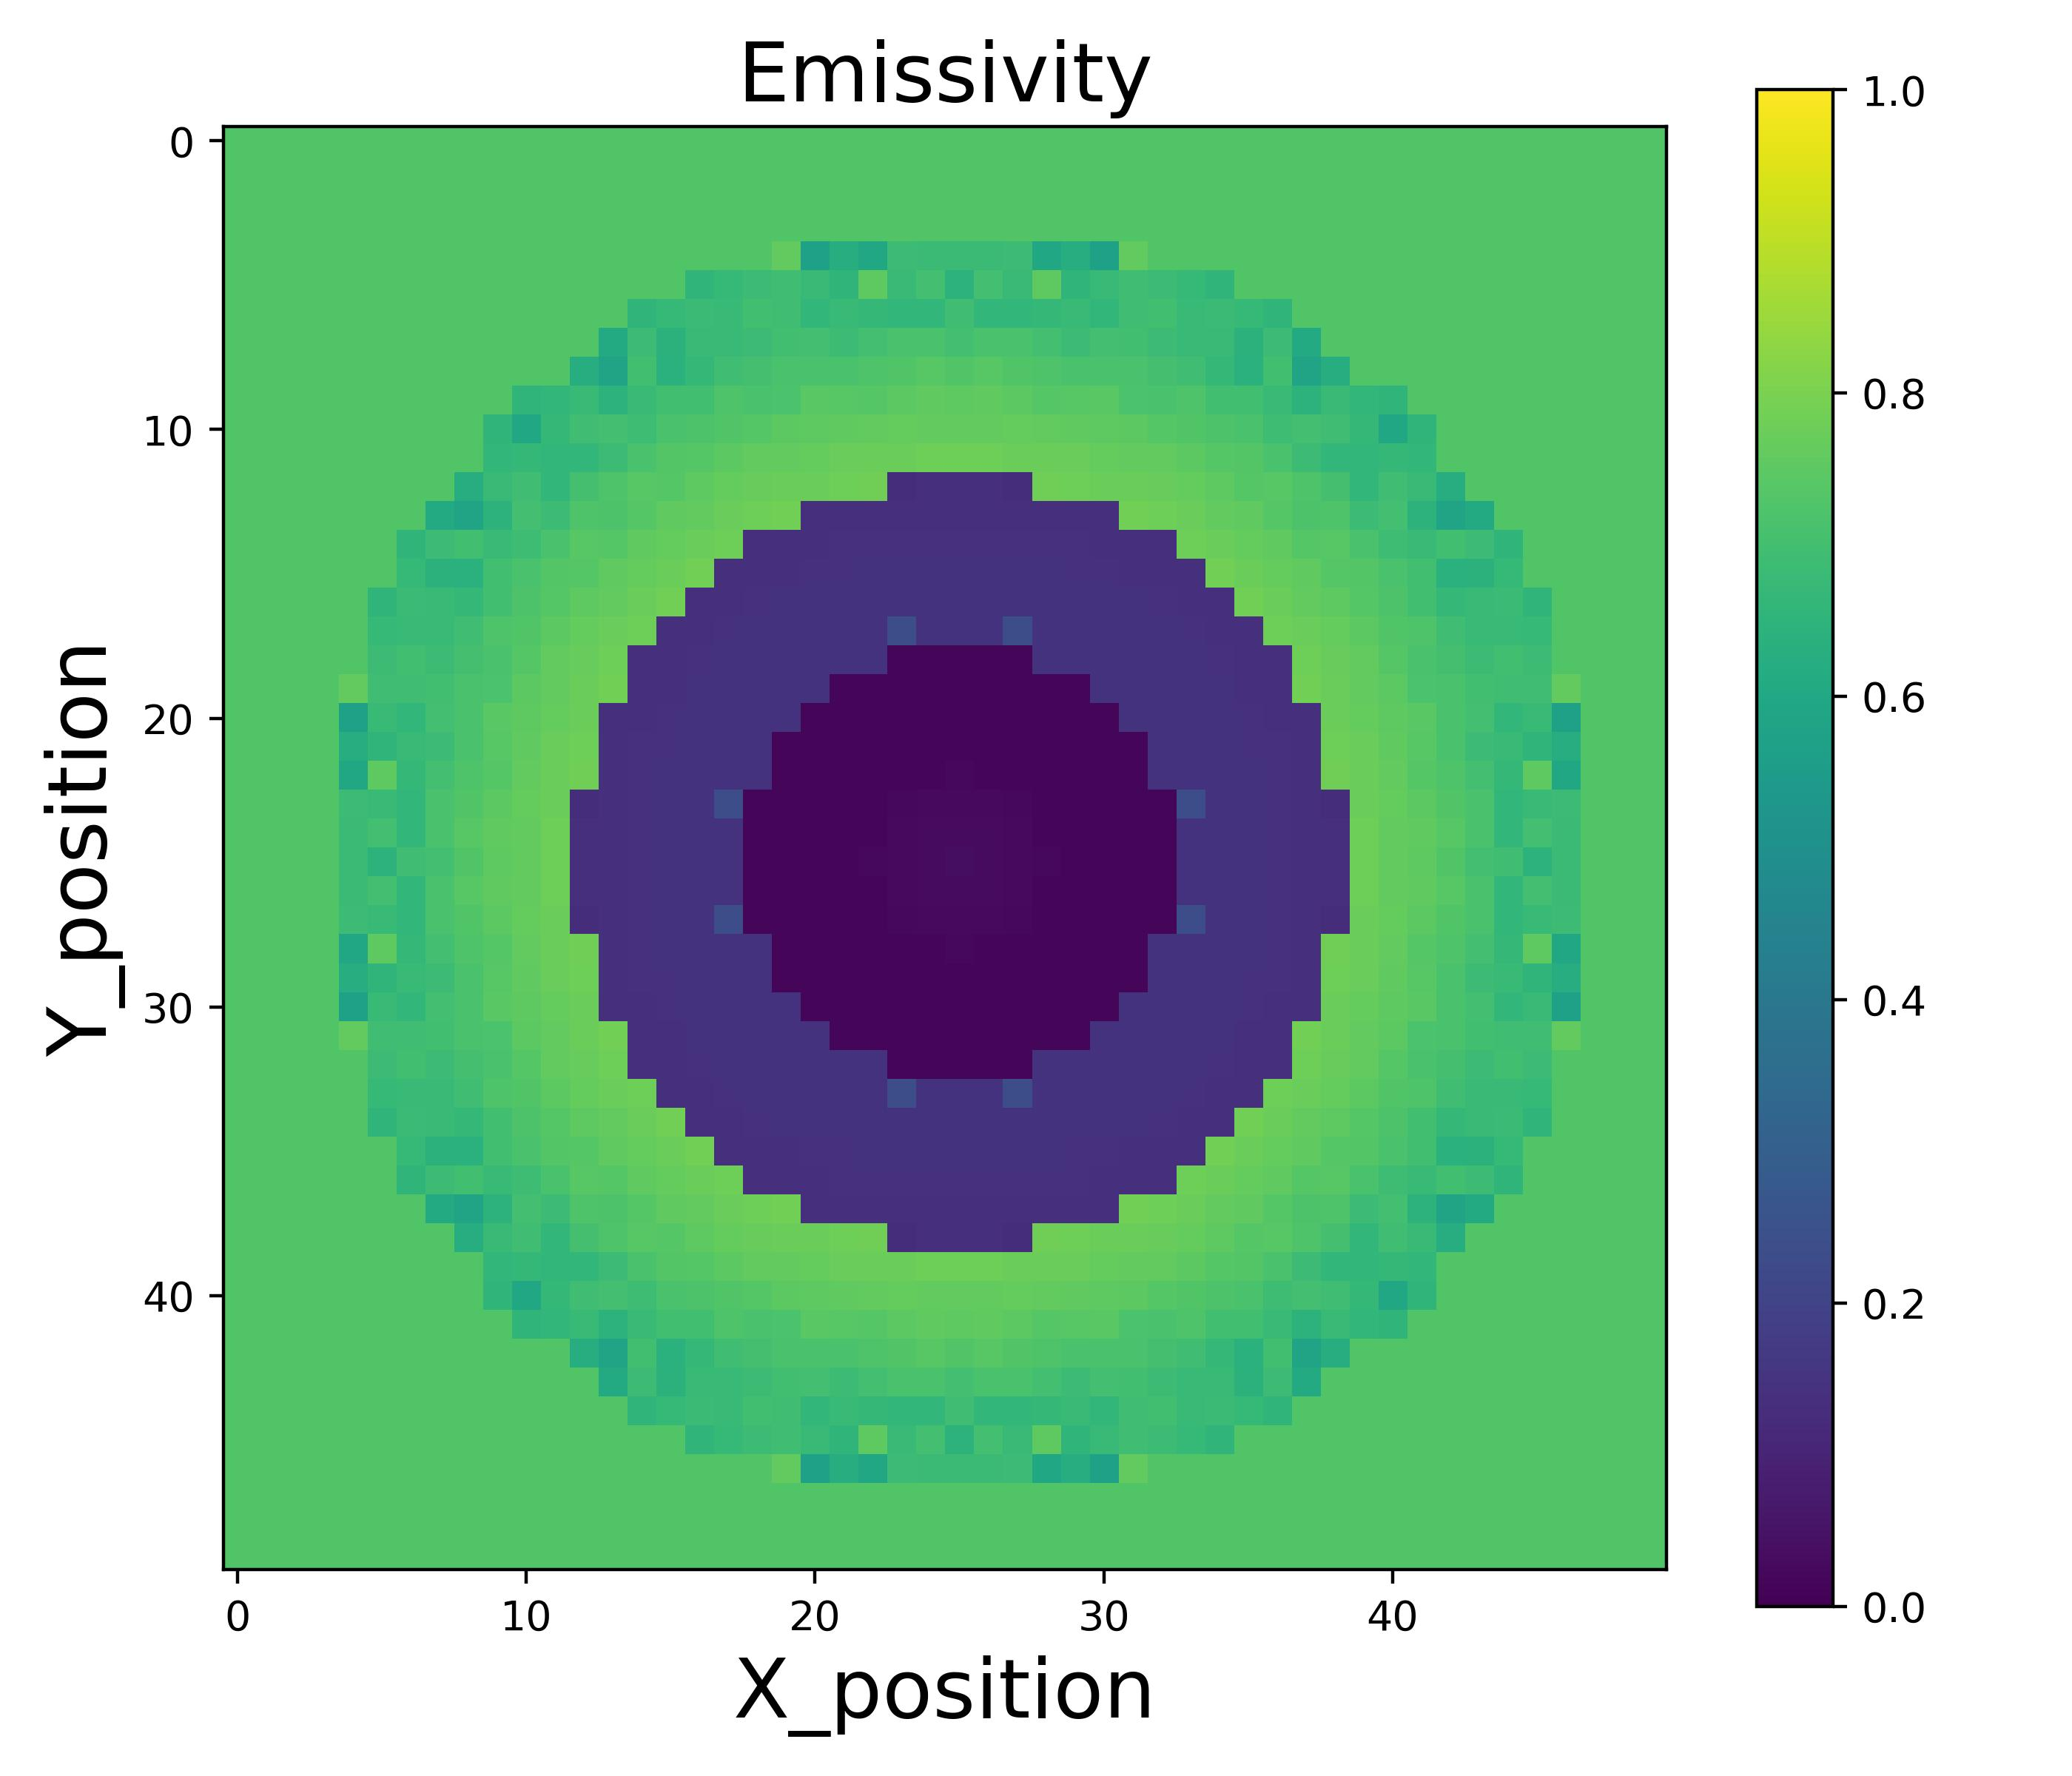
\includegraphics[width=\textwidth]{figures/raw_data/24/linear/emi_cal.jpg}
            \subcaption{Model 4}
        \end{subfigure}
    \end{minipage}\\
    \begin{minipage}{\textwidth}
        \centering
        \begin{subfigure}{0.325\textwidth}
            \centering
            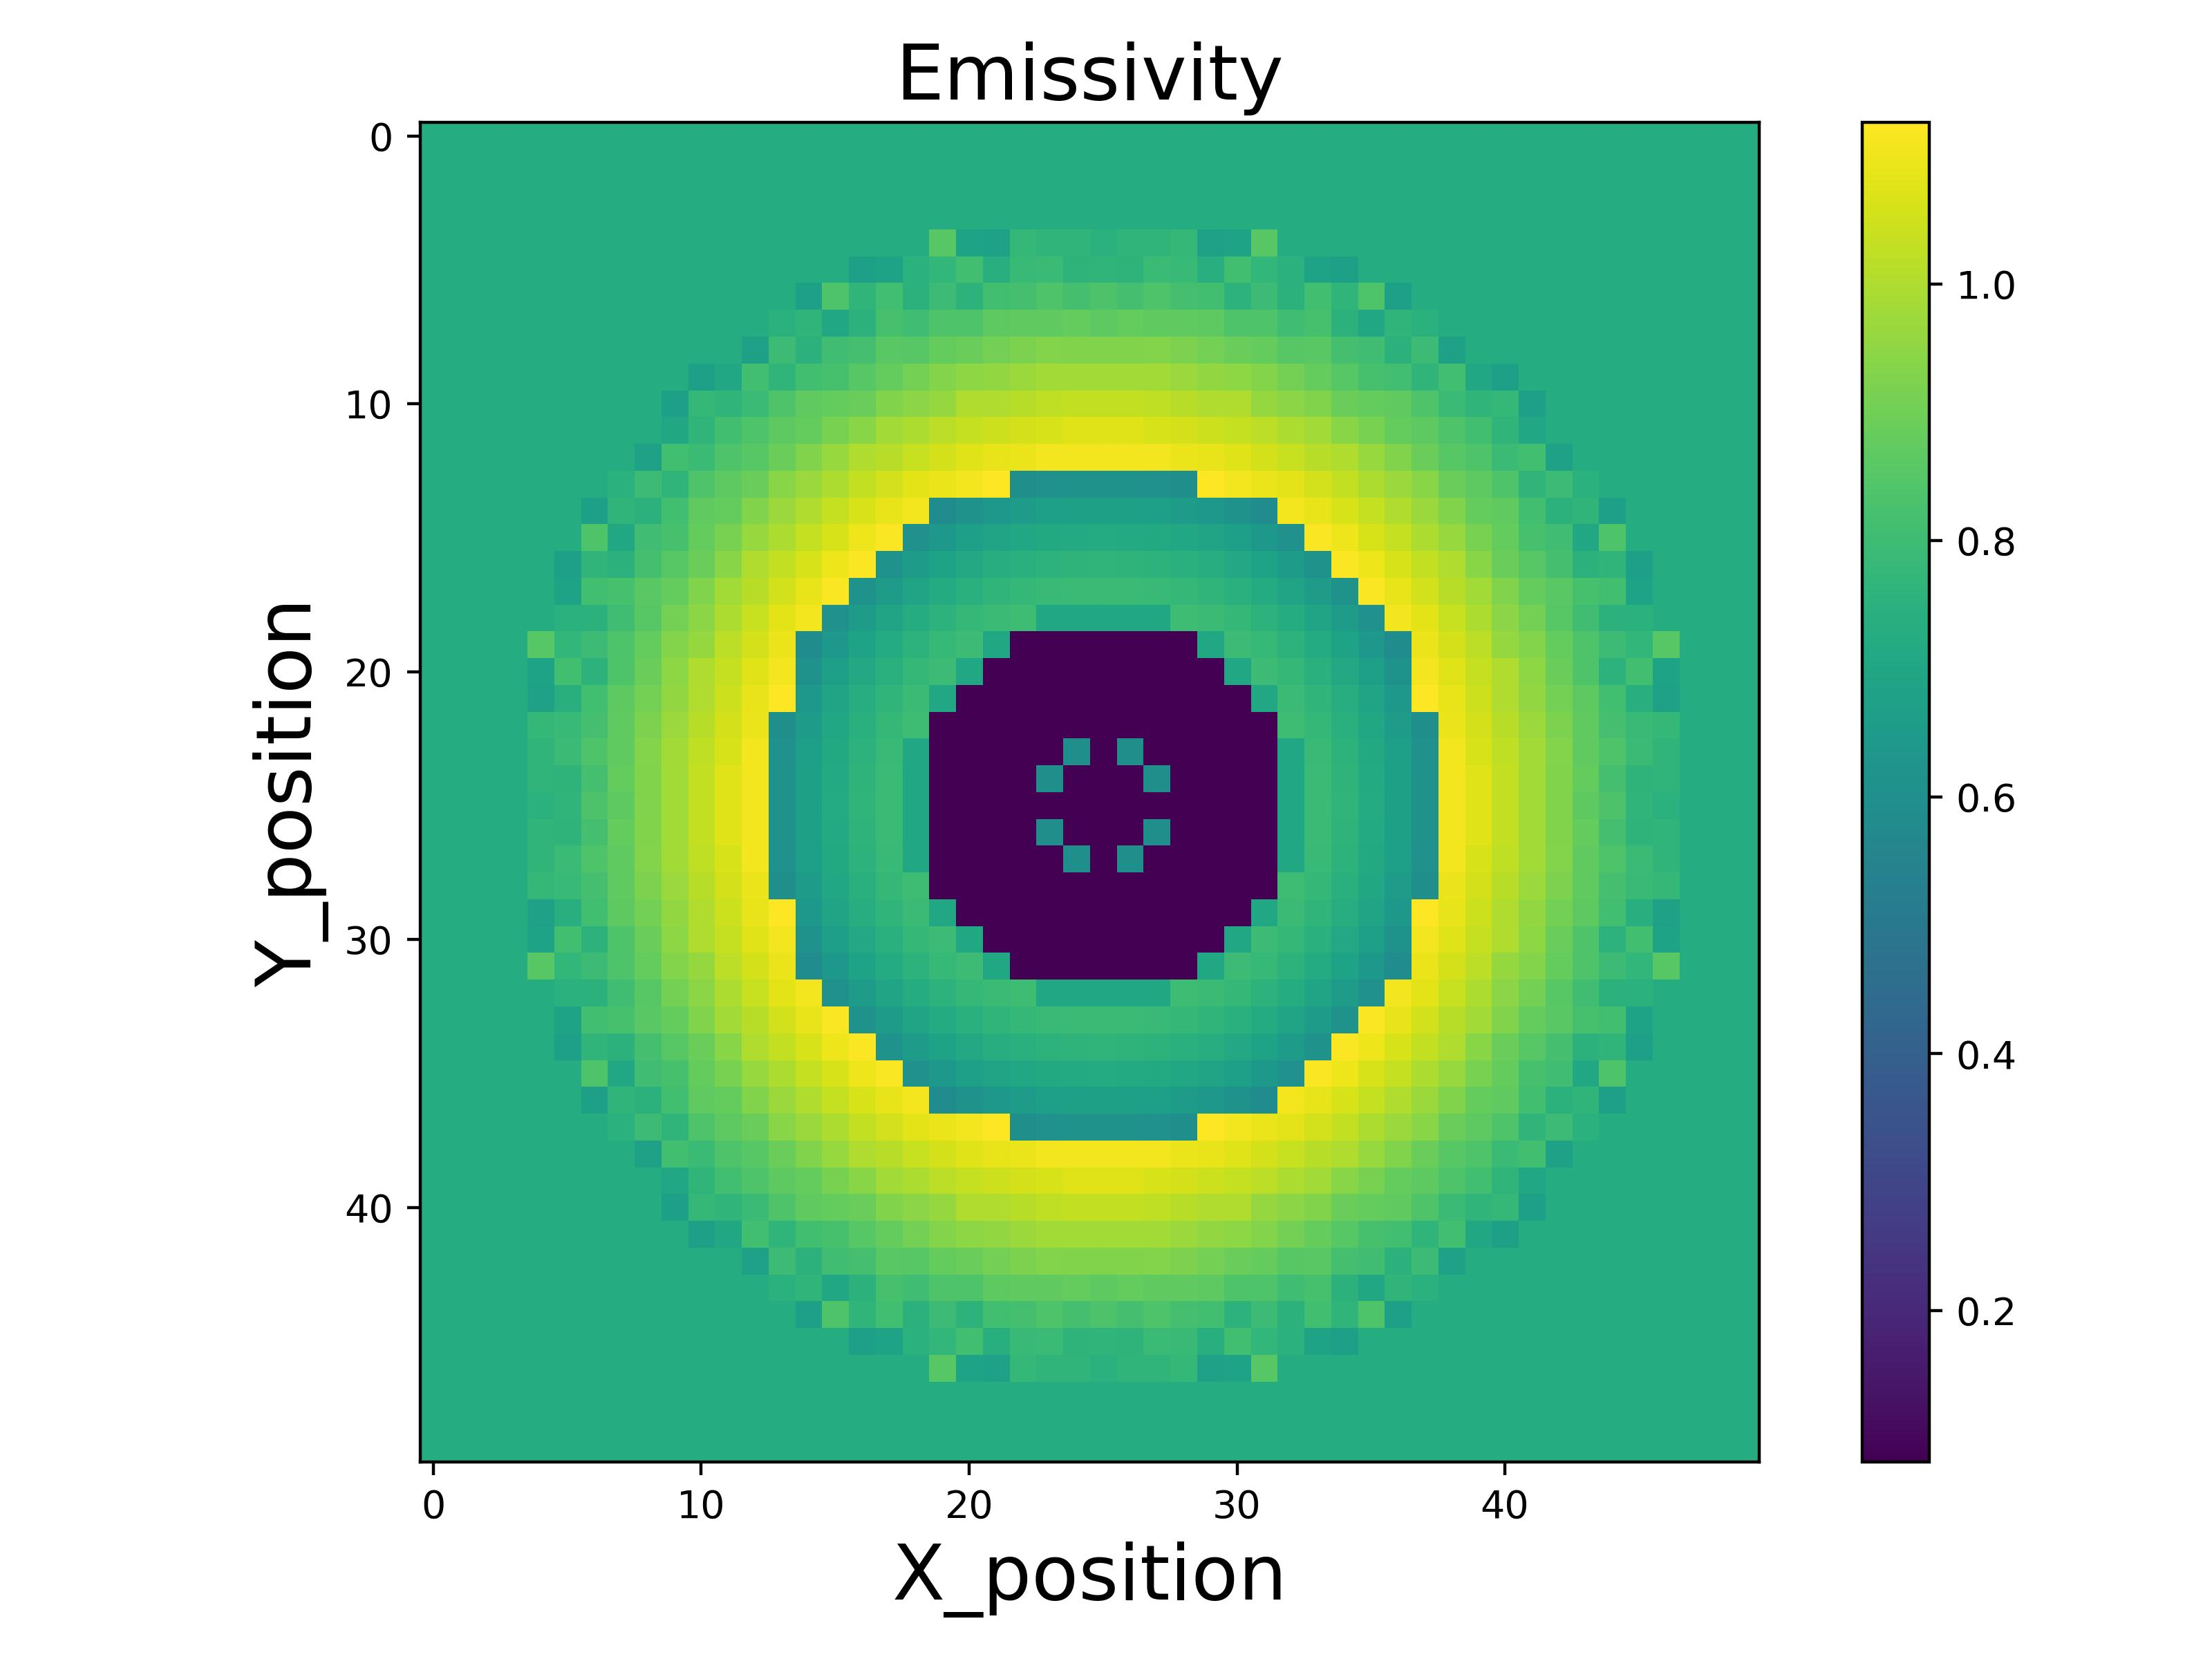
\includegraphics[width=\textwidth]{figures/raw_data/25/linear/emi_cal.jpg}
            \subcaption{Model 5}
        \end{subfigure}
        \begin{subfigure}{0.325\textwidth}
            \centering
            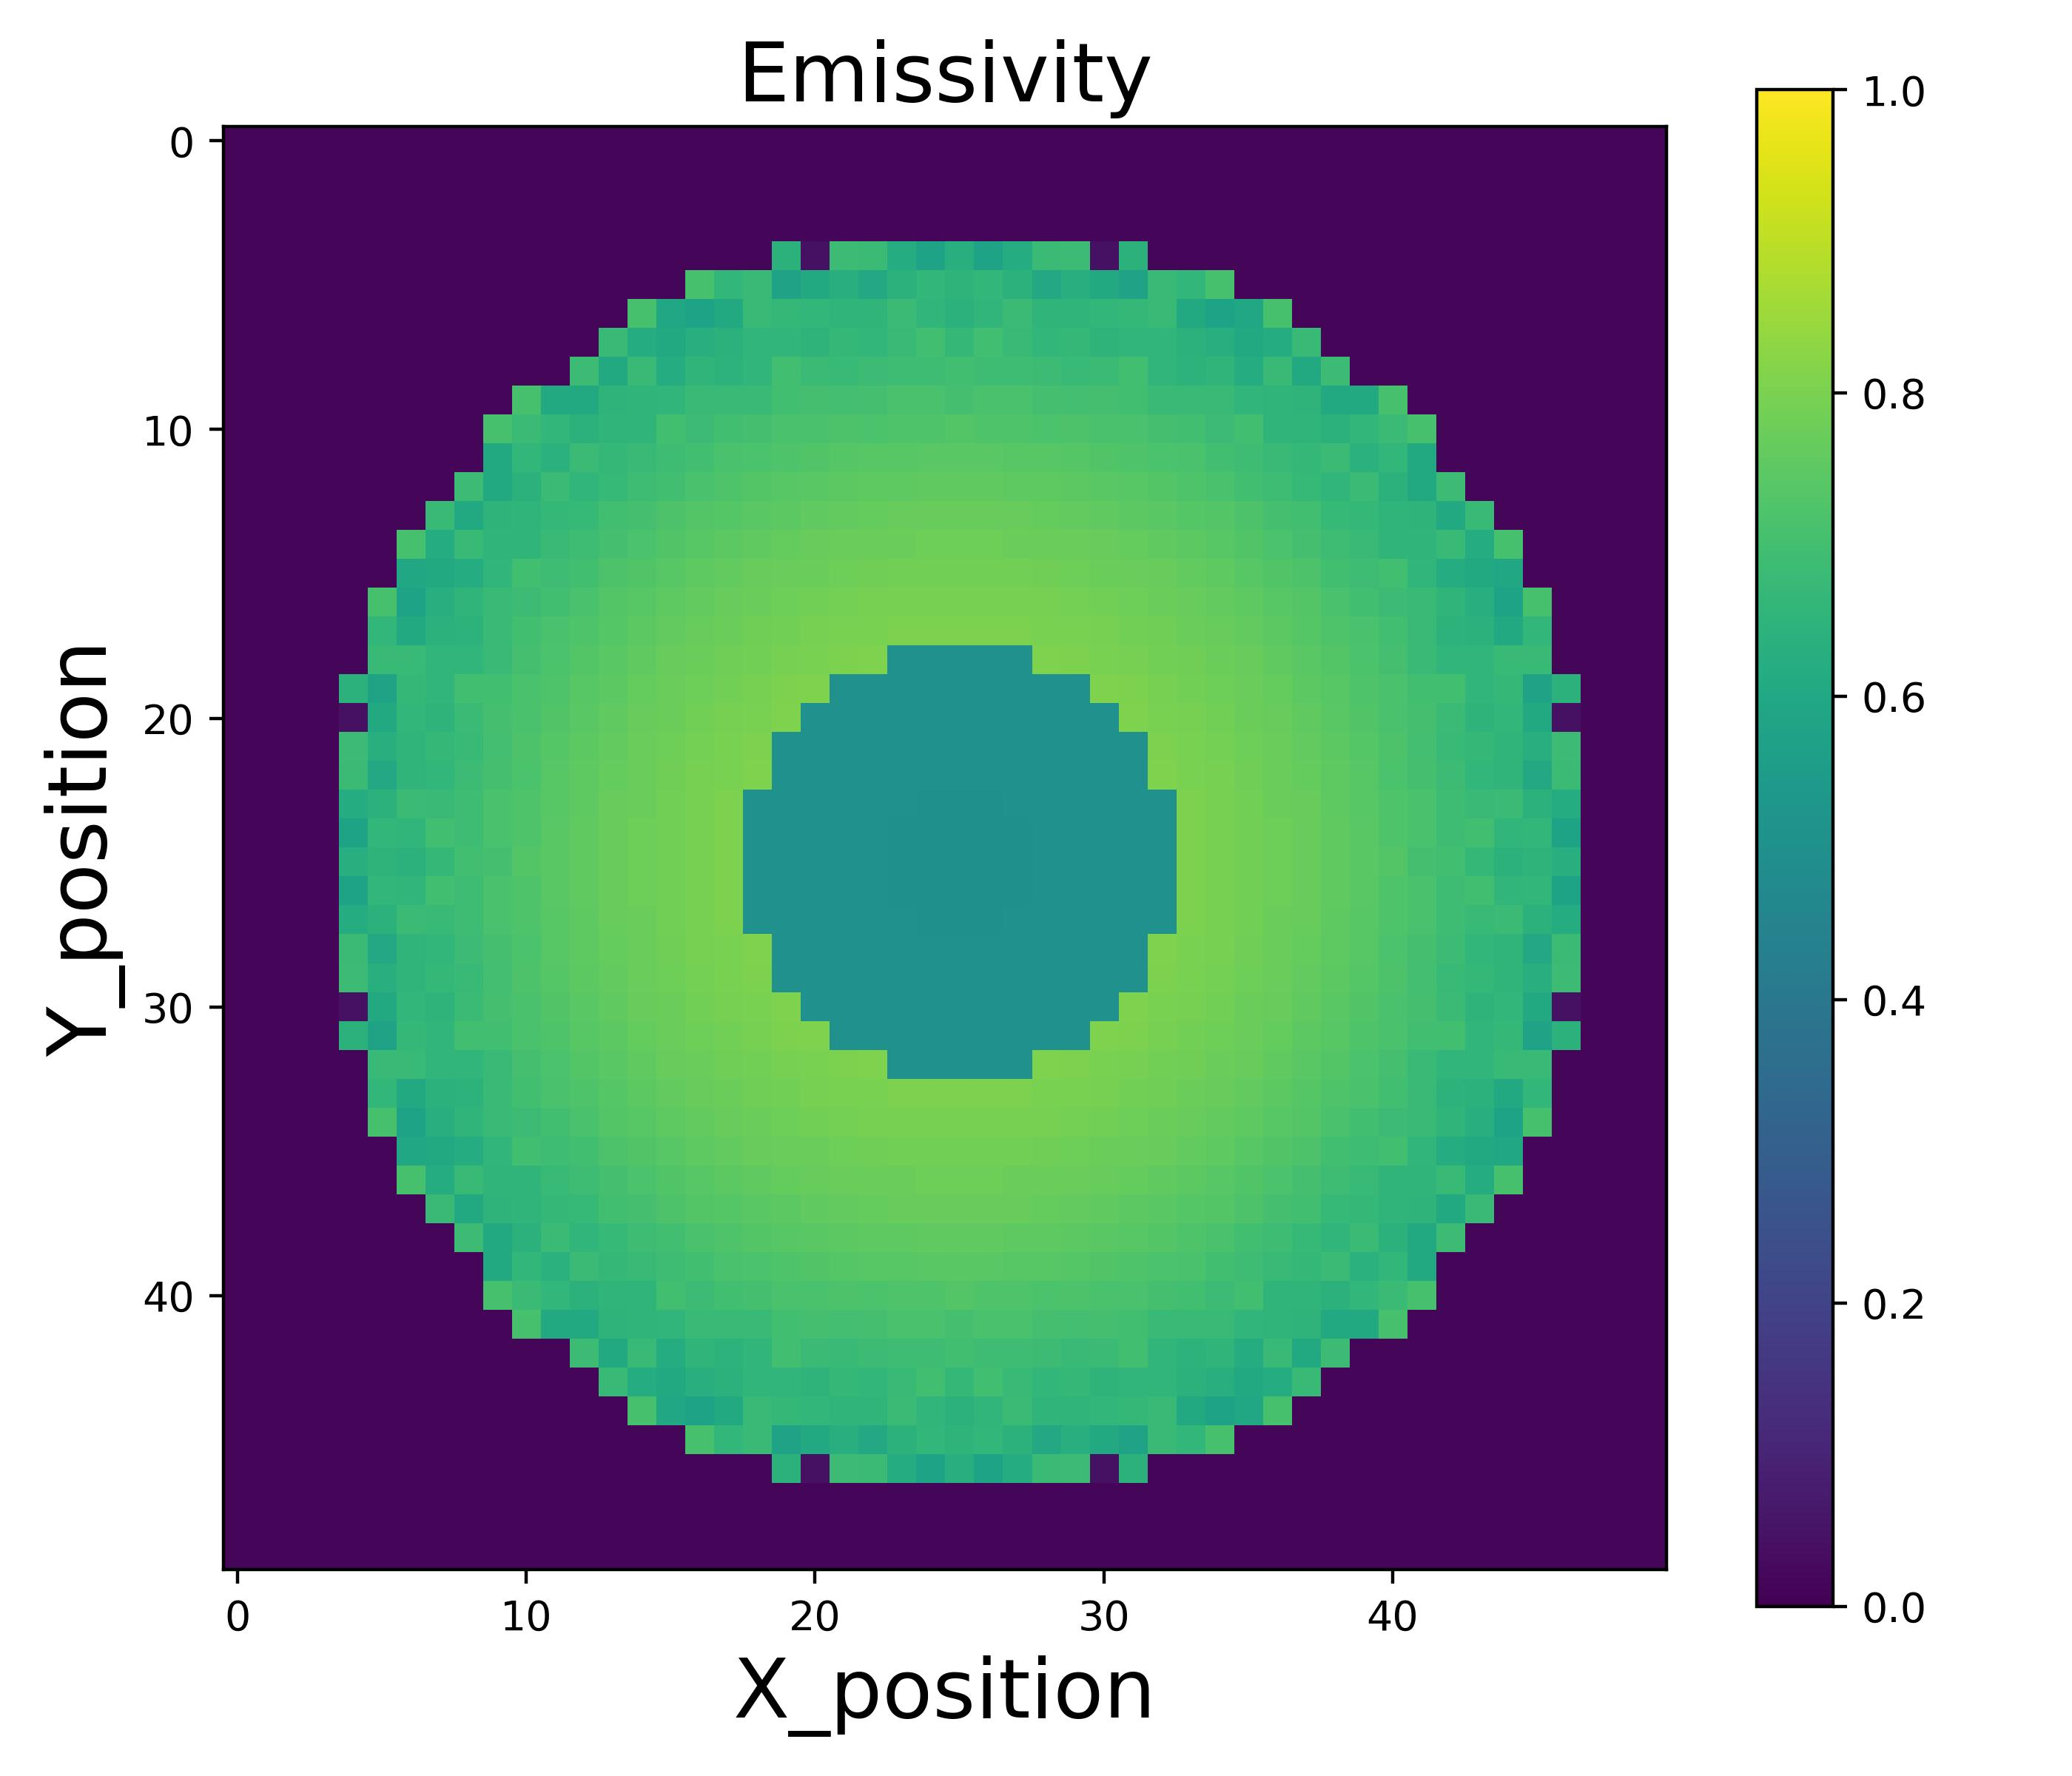
\includegraphics[width=\textwidth]{figures/raw_data/26/linear/emi_cal.jpg}
            \subcaption{Model 6}
        \end{subfigure}
        \begin{subfigure}{0.325\textwidth}
            \centering
            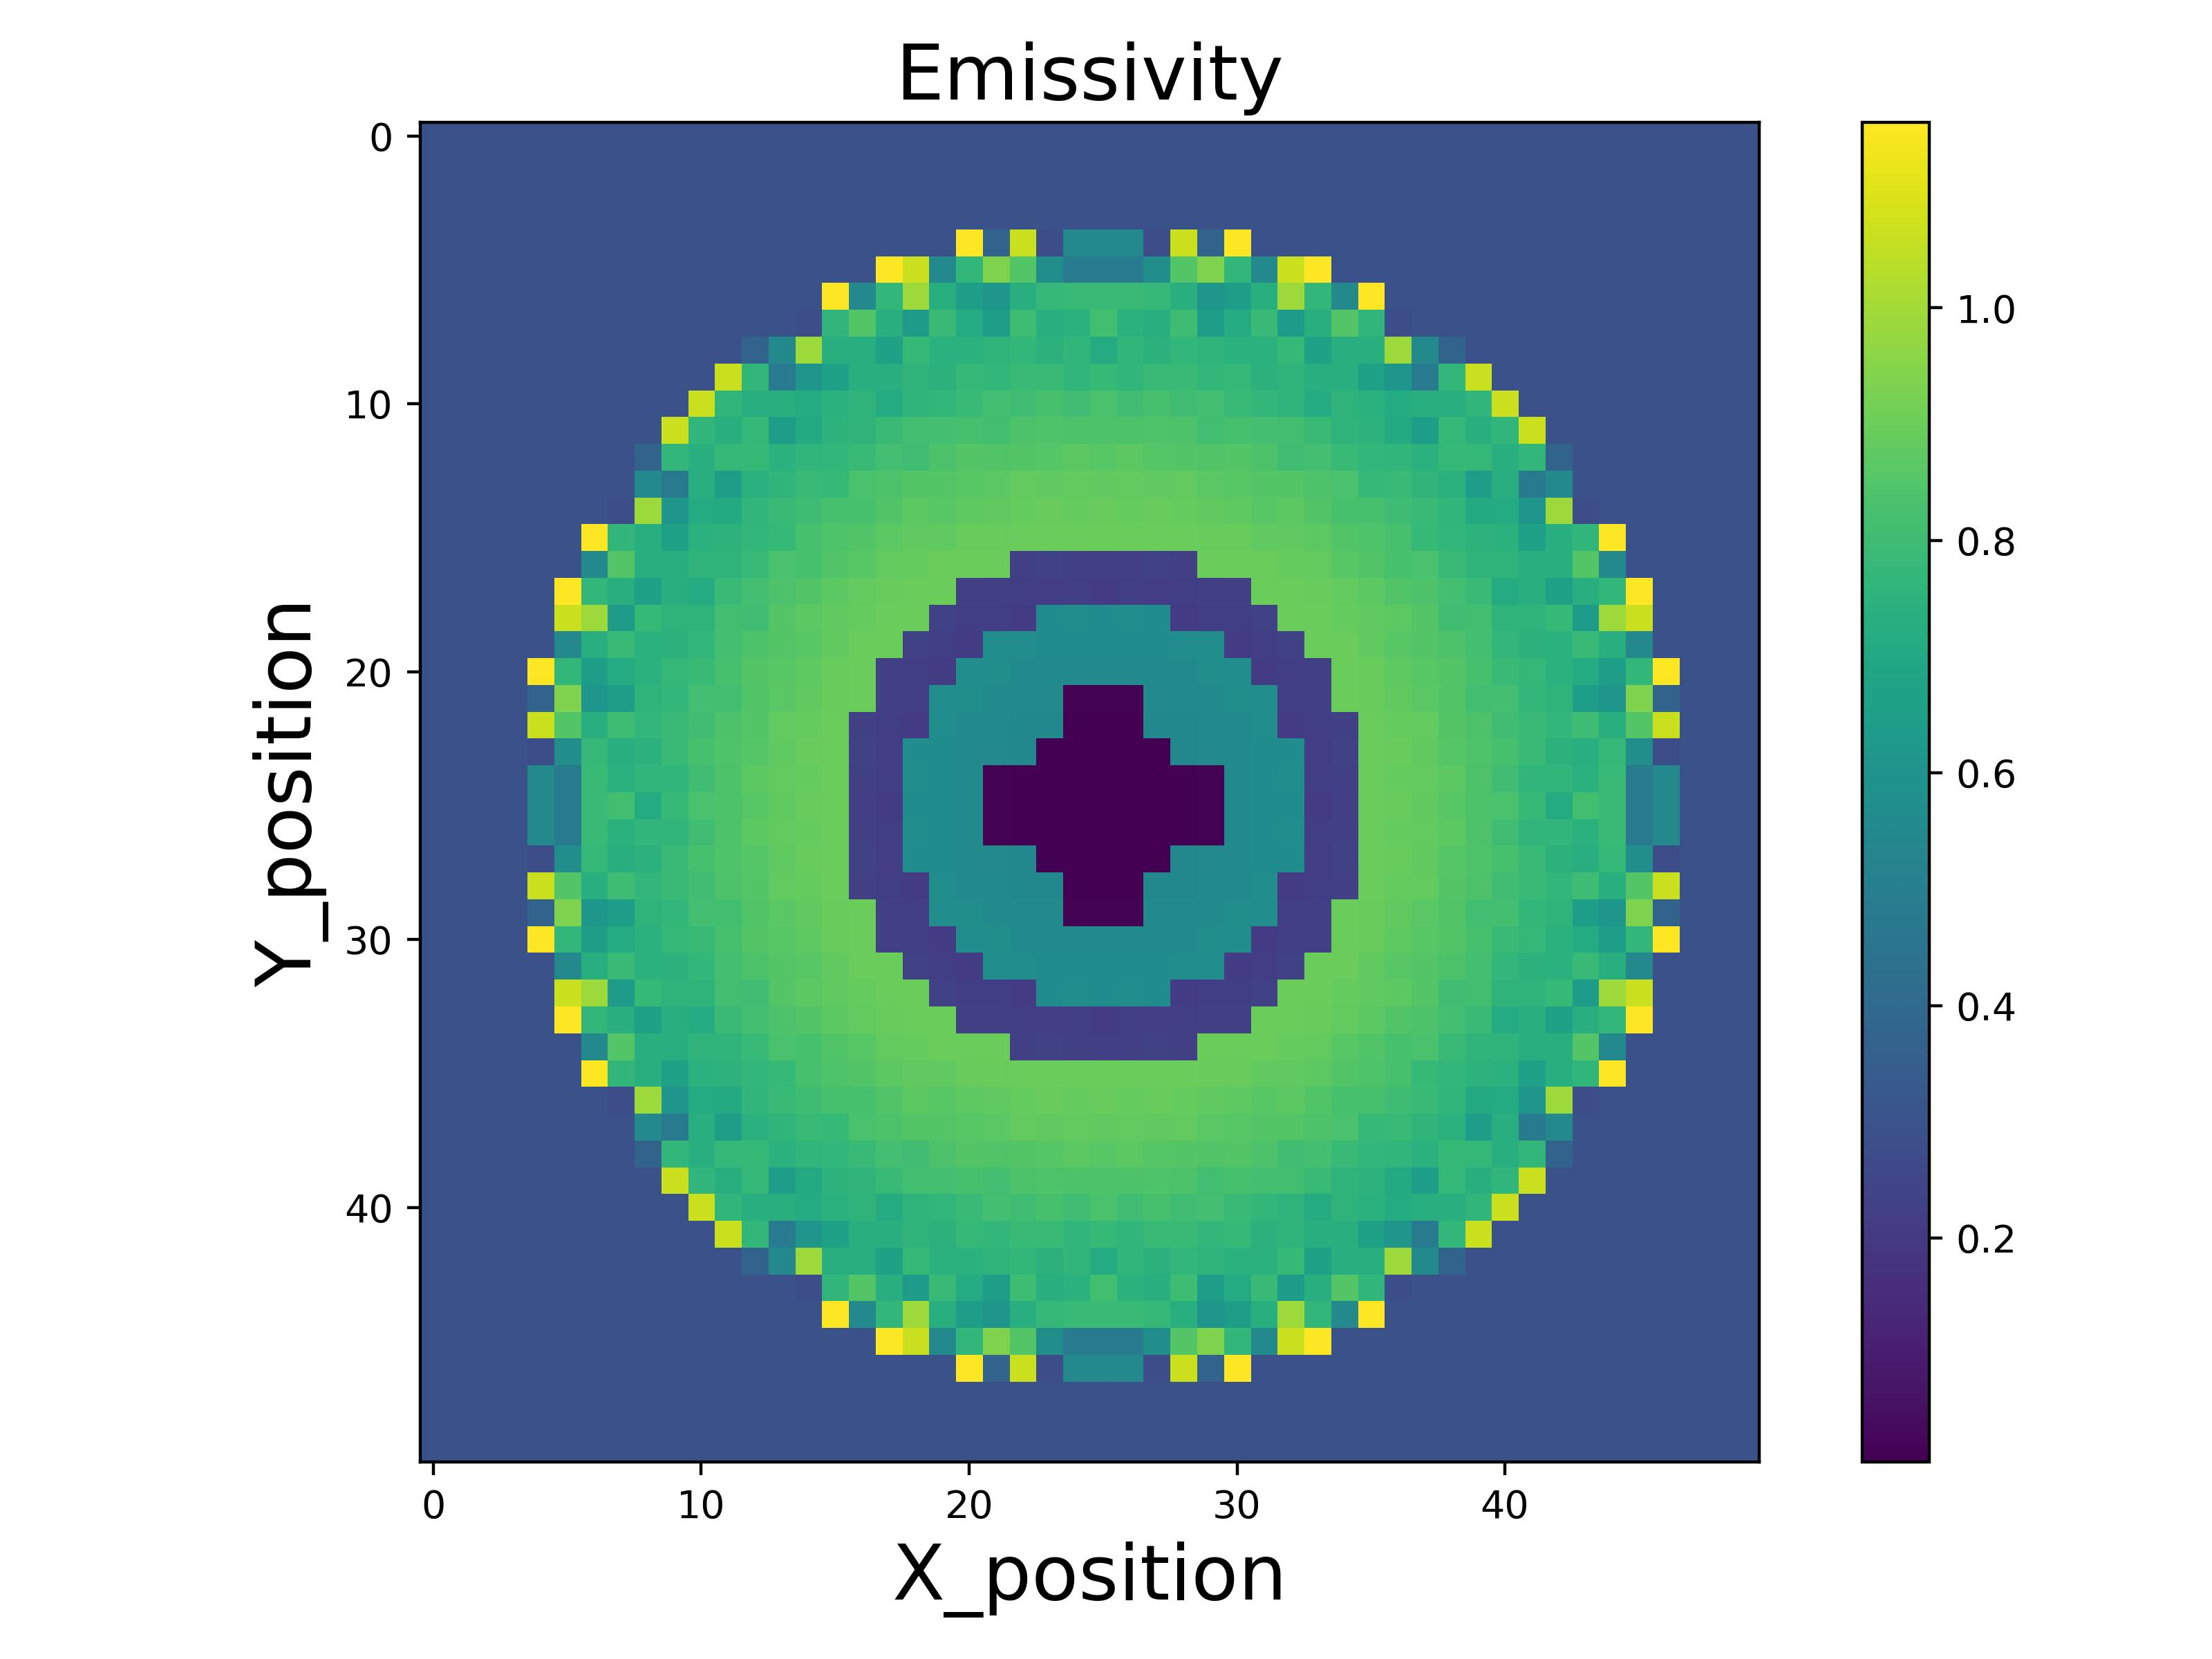
\includegraphics[width=\textwidth]{figures/raw_data/31/linear/emi_cal.jpg}
            \subcaption{Model 7}
        \end{subfigure}
    \end{minipage}\\
    \begin{minipage}{\textwidth}
        \centering
        \begin{subfigure}{0.325\textwidth}
            \centering
            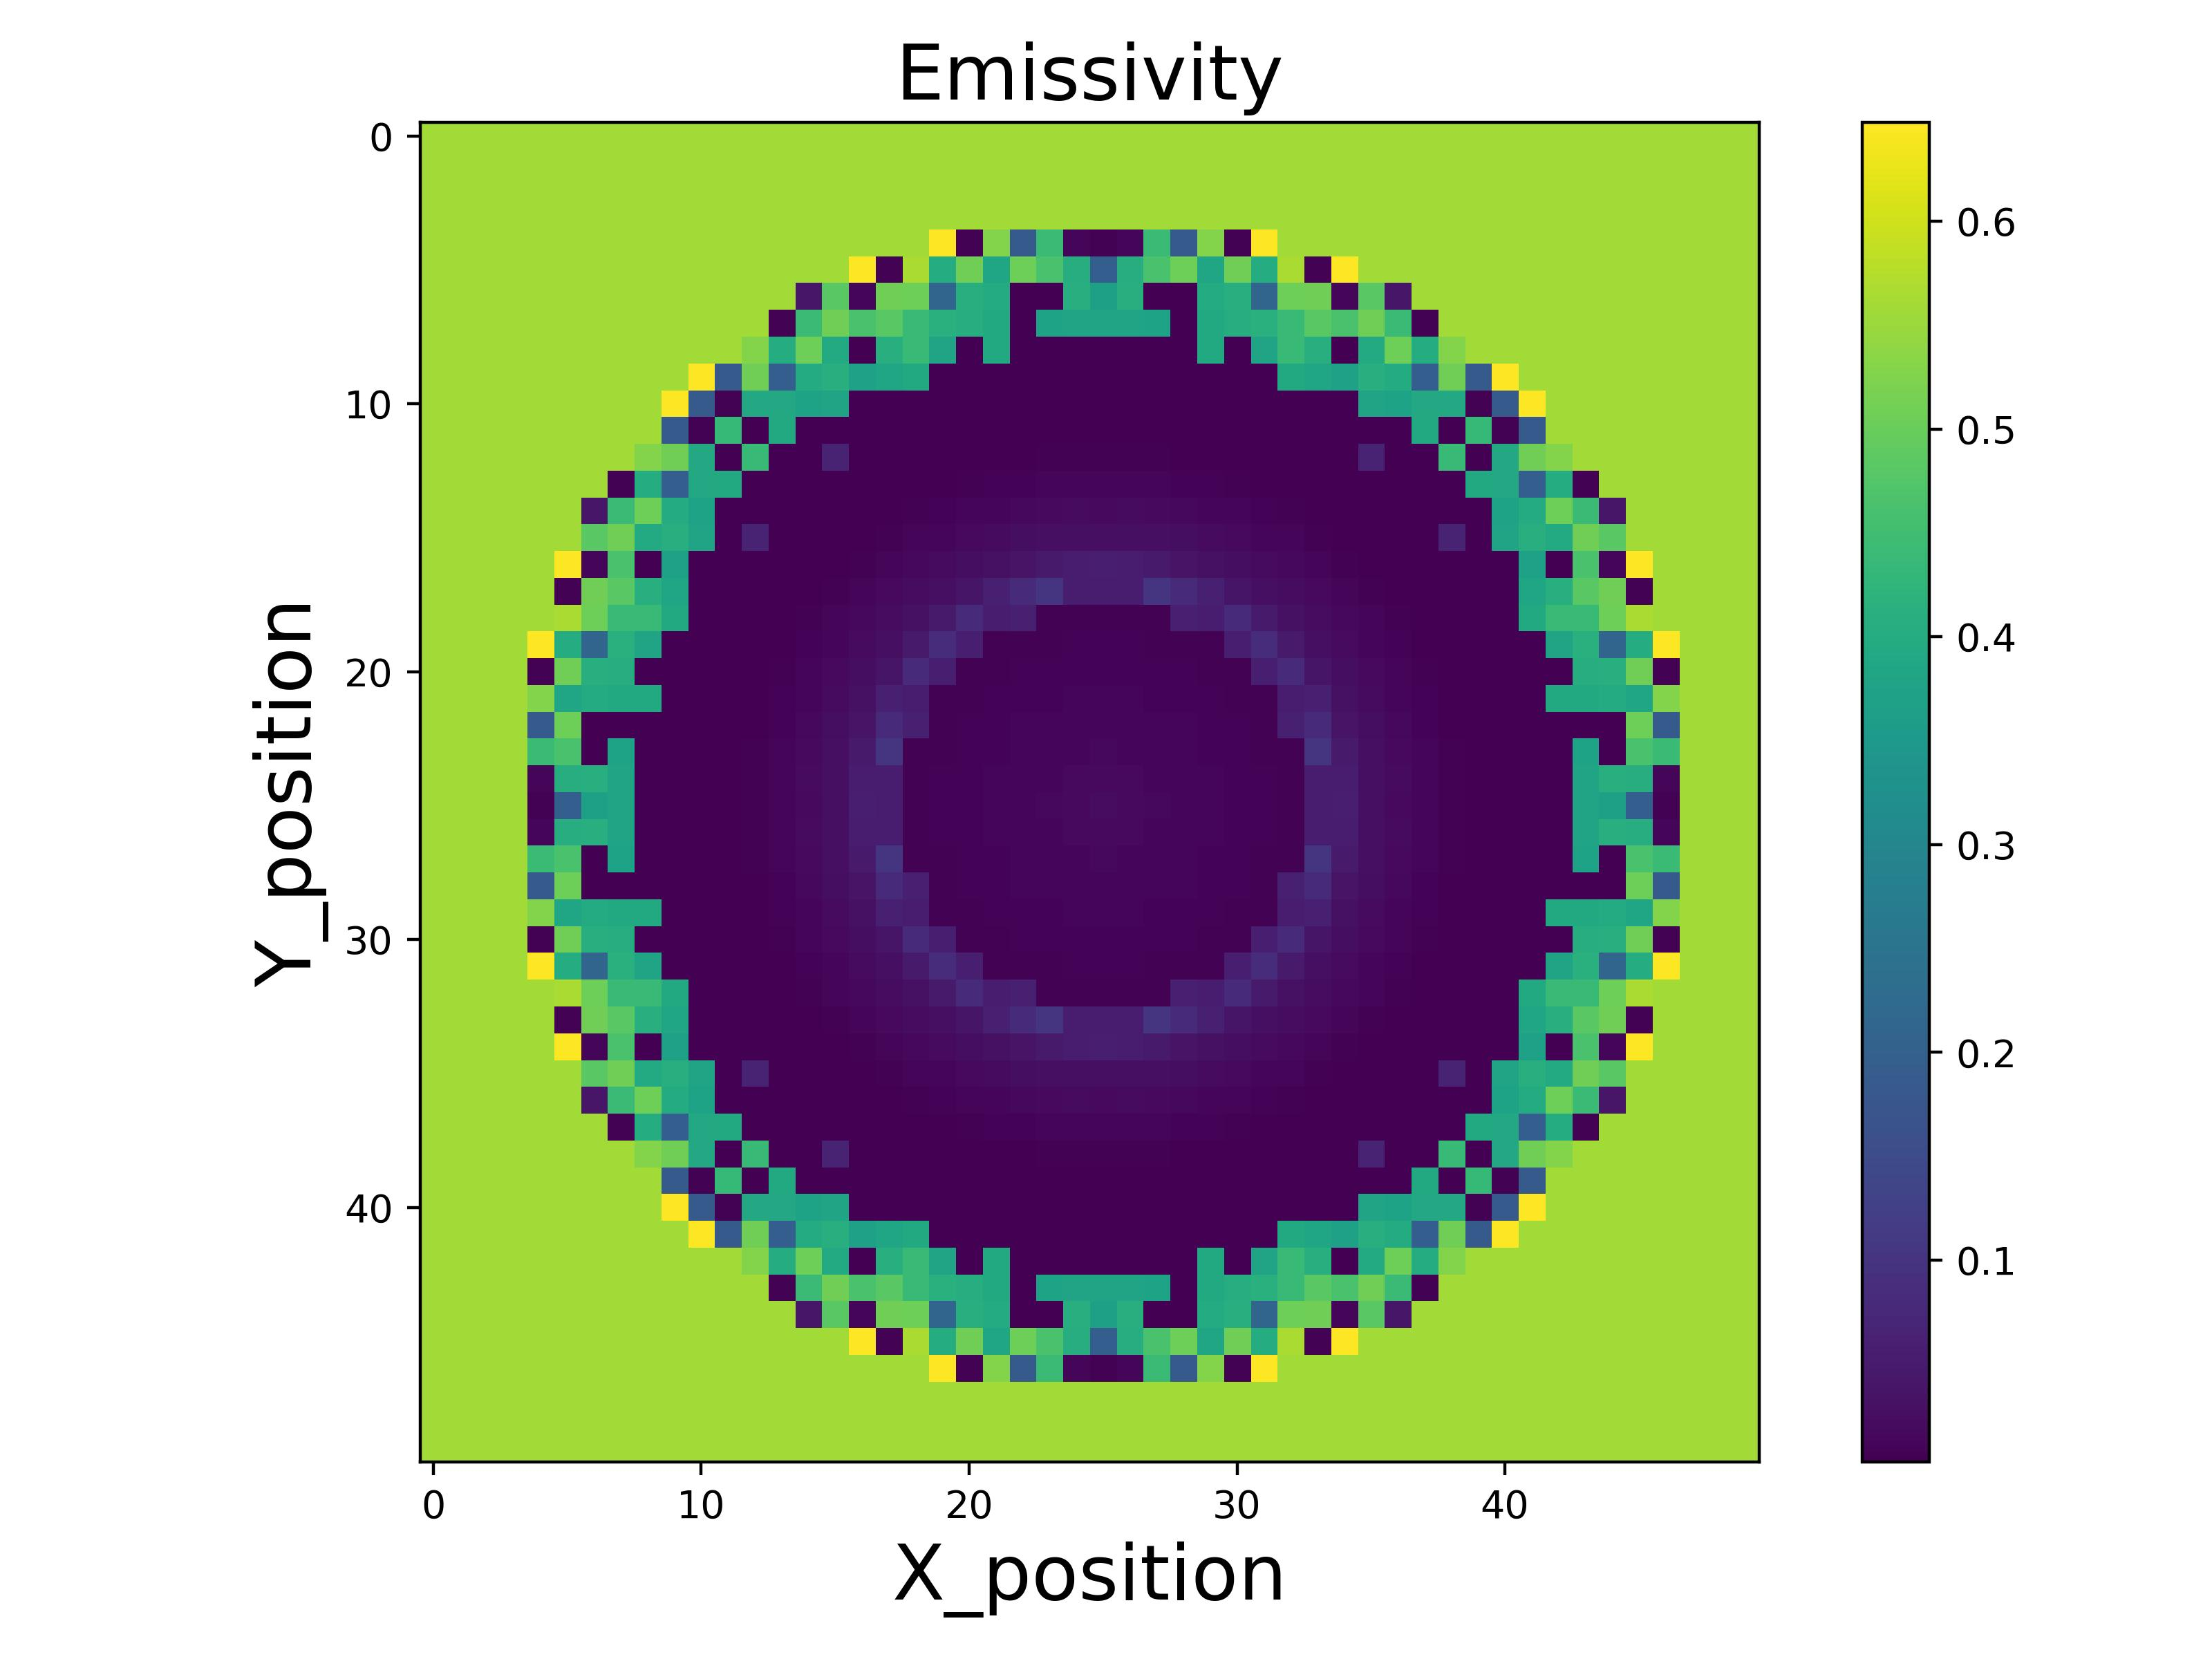
\includegraphics[width=\textwidth]{figures/raw_data/32/linear/emi_cal.jpg}
            \subcaption{Model 8}
        \end{subfigure}
        \begin{subfigure}{0.325\textwidth}
            \centering
            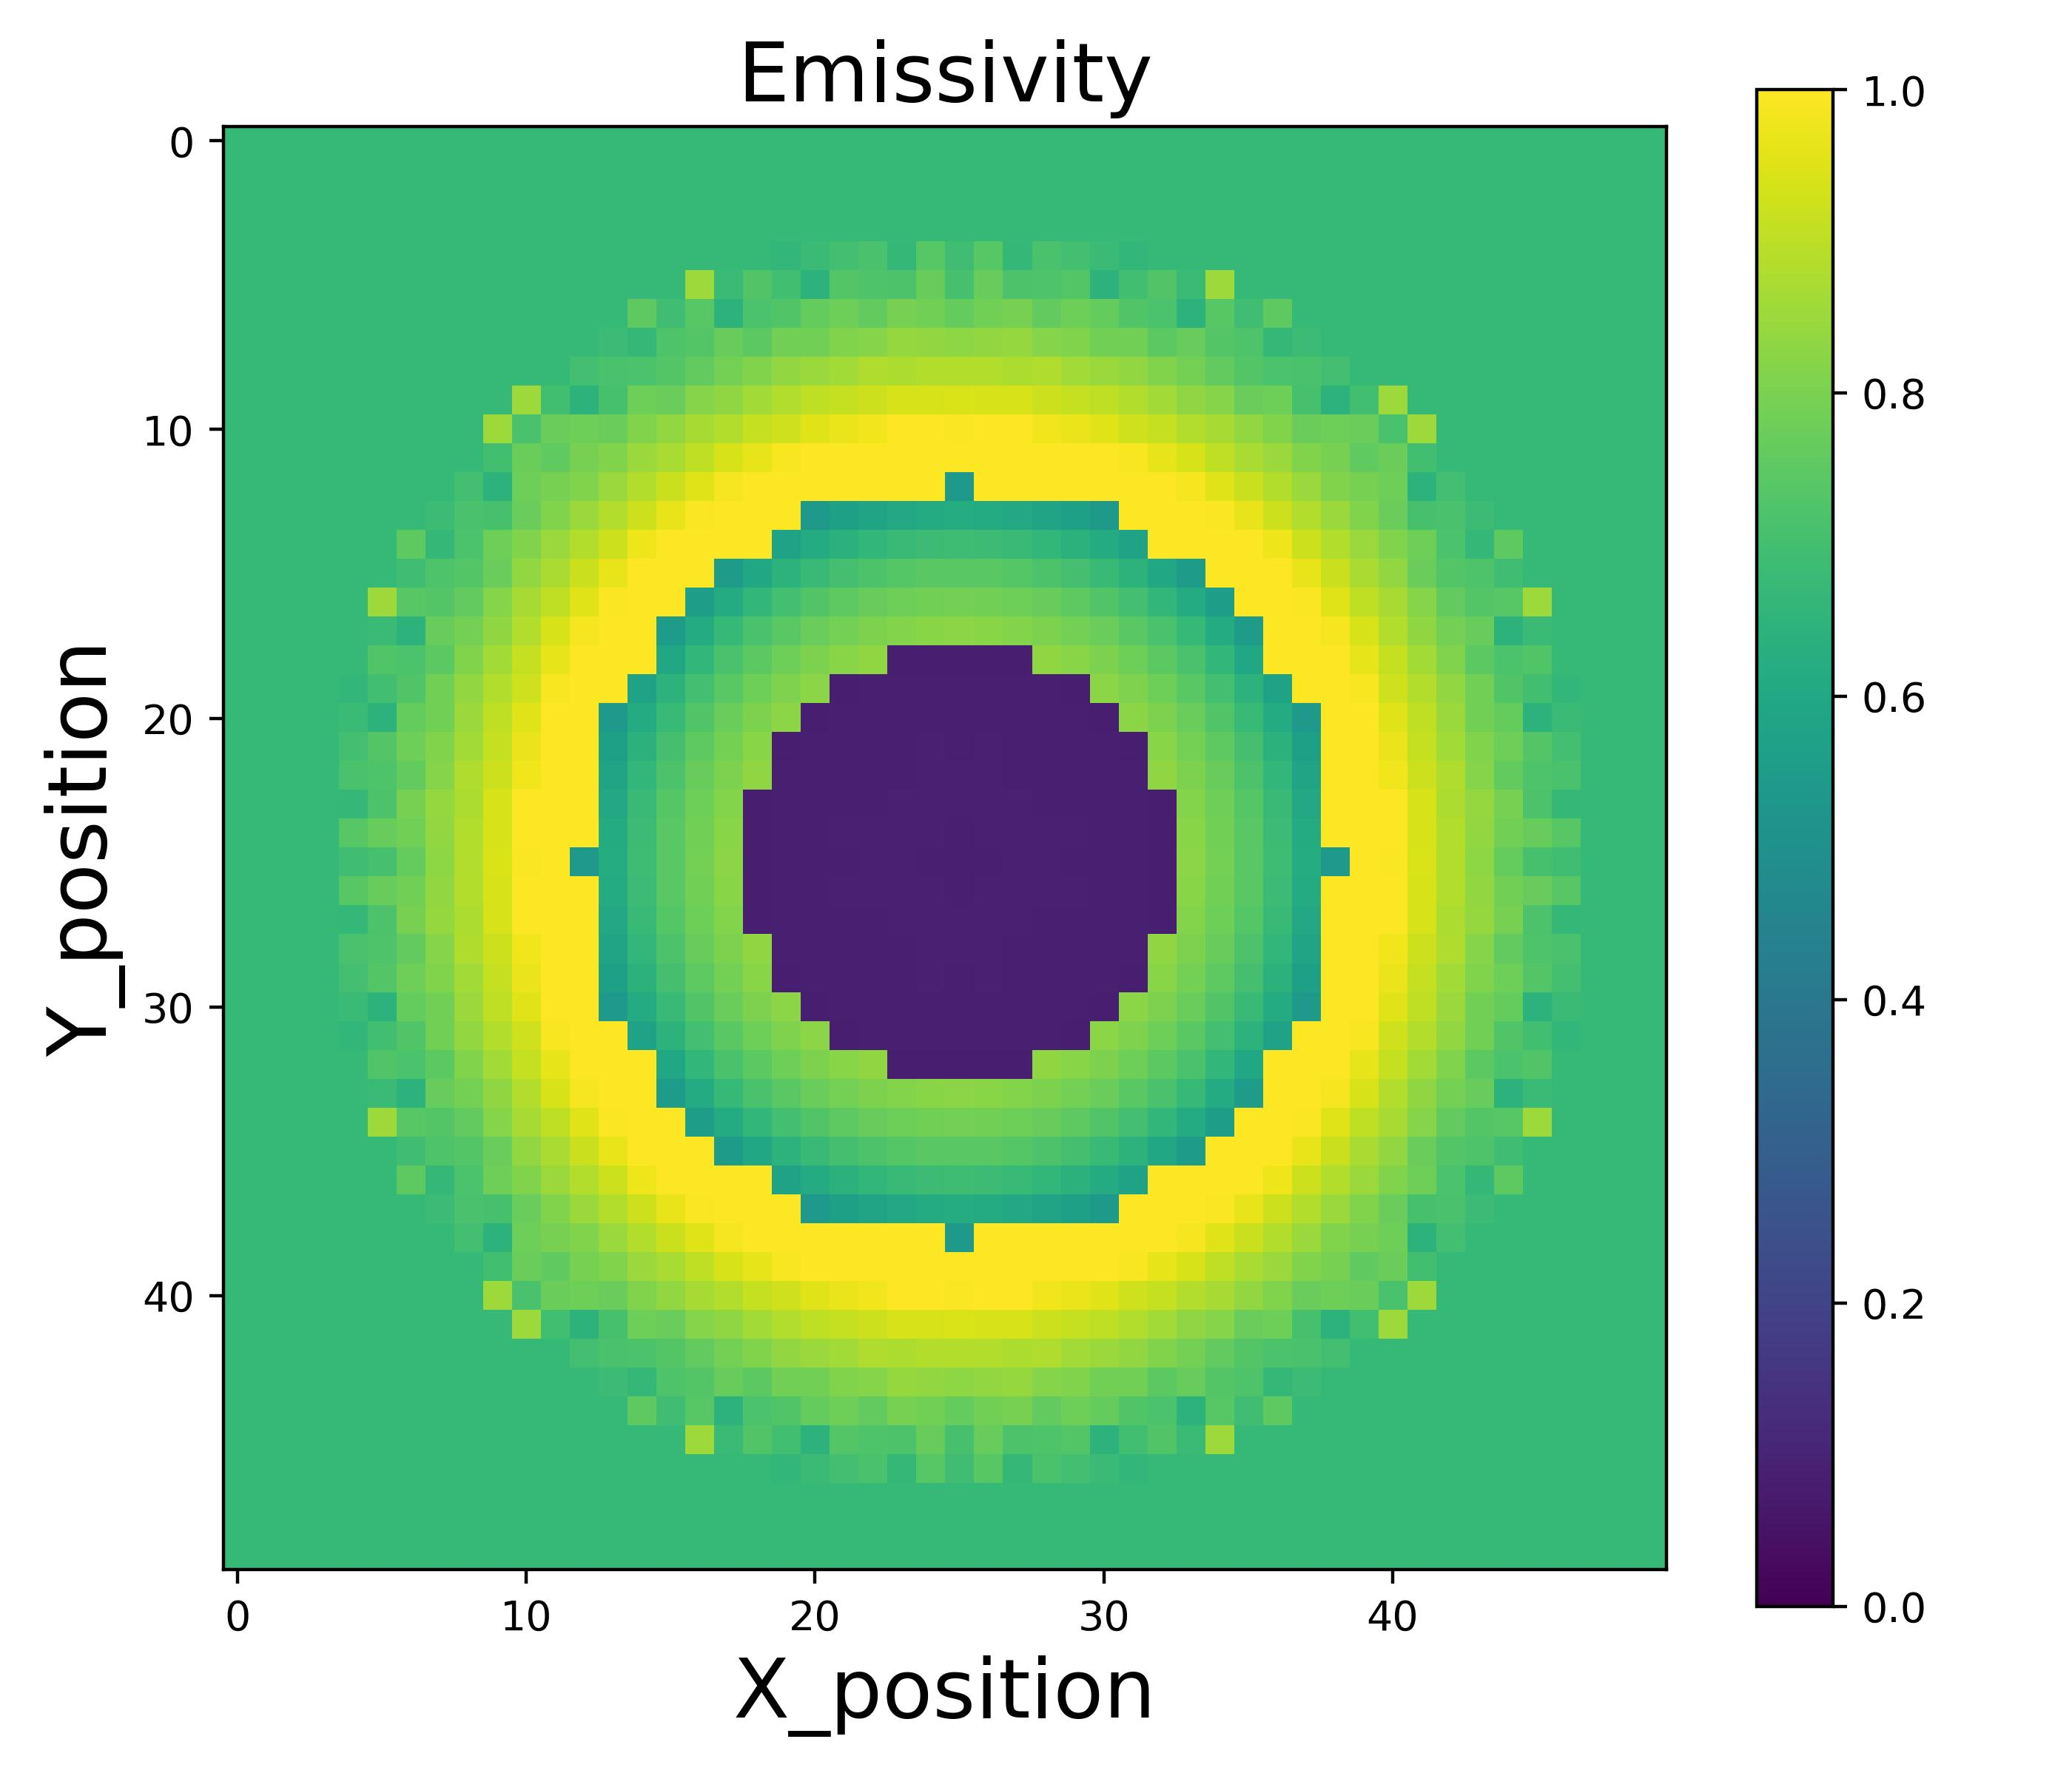
\includegraphics[width=\textwidth]{figures/raw_data/33/linear/emi_cal.jpg}
            \subcaption{Model 9}
        \end{subfigure}
    \end{minipage}
    \caption{Emissivity calculation results of linear model}  
\end{figure}


\newpage
\subsection{Linear square model}
\begin{figure}[h]
    \centering
    \begin{minipage}{\textwidth}
        \centering
        \begin{subfigure}{0.27\textwidth}
            \centering
            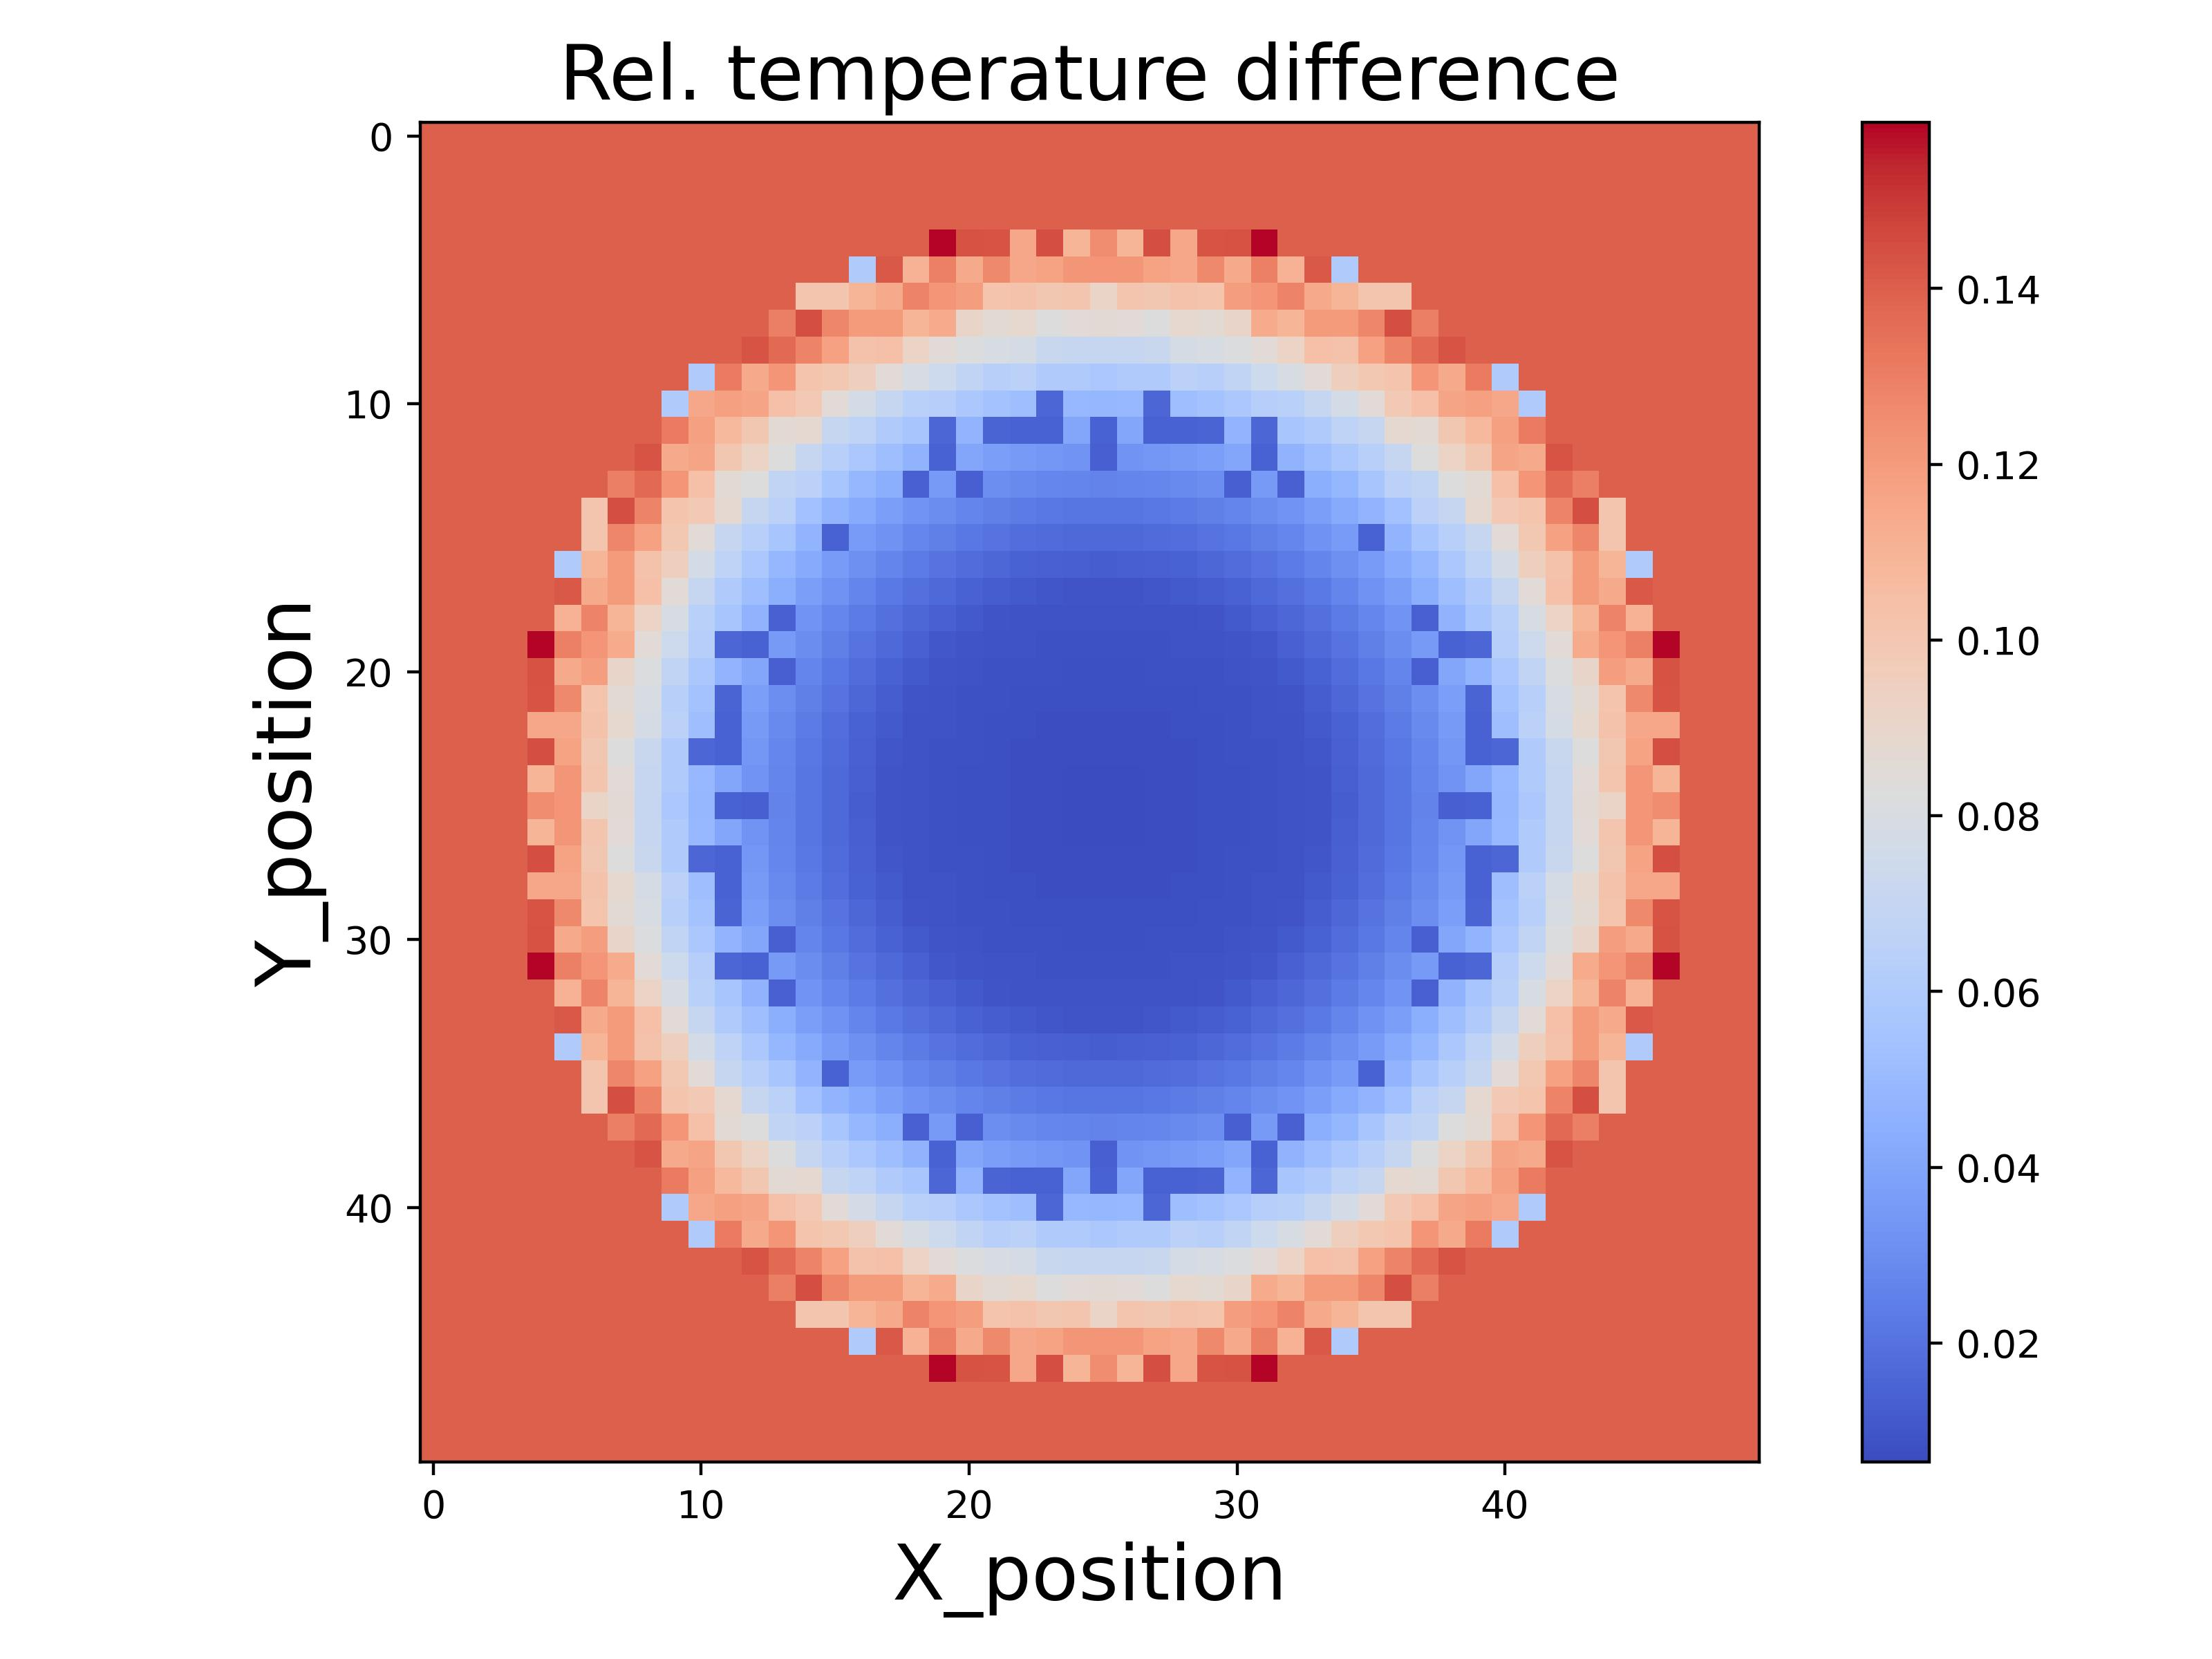
\includegraphics[width=\textwidth]{figures/raw_data/0/lin_square/T_bias.jpg}
            \subcaption{Black body material}
        \end{subfigure}
        \begin{subfigure}{0.27\textwidth}
            \centering
            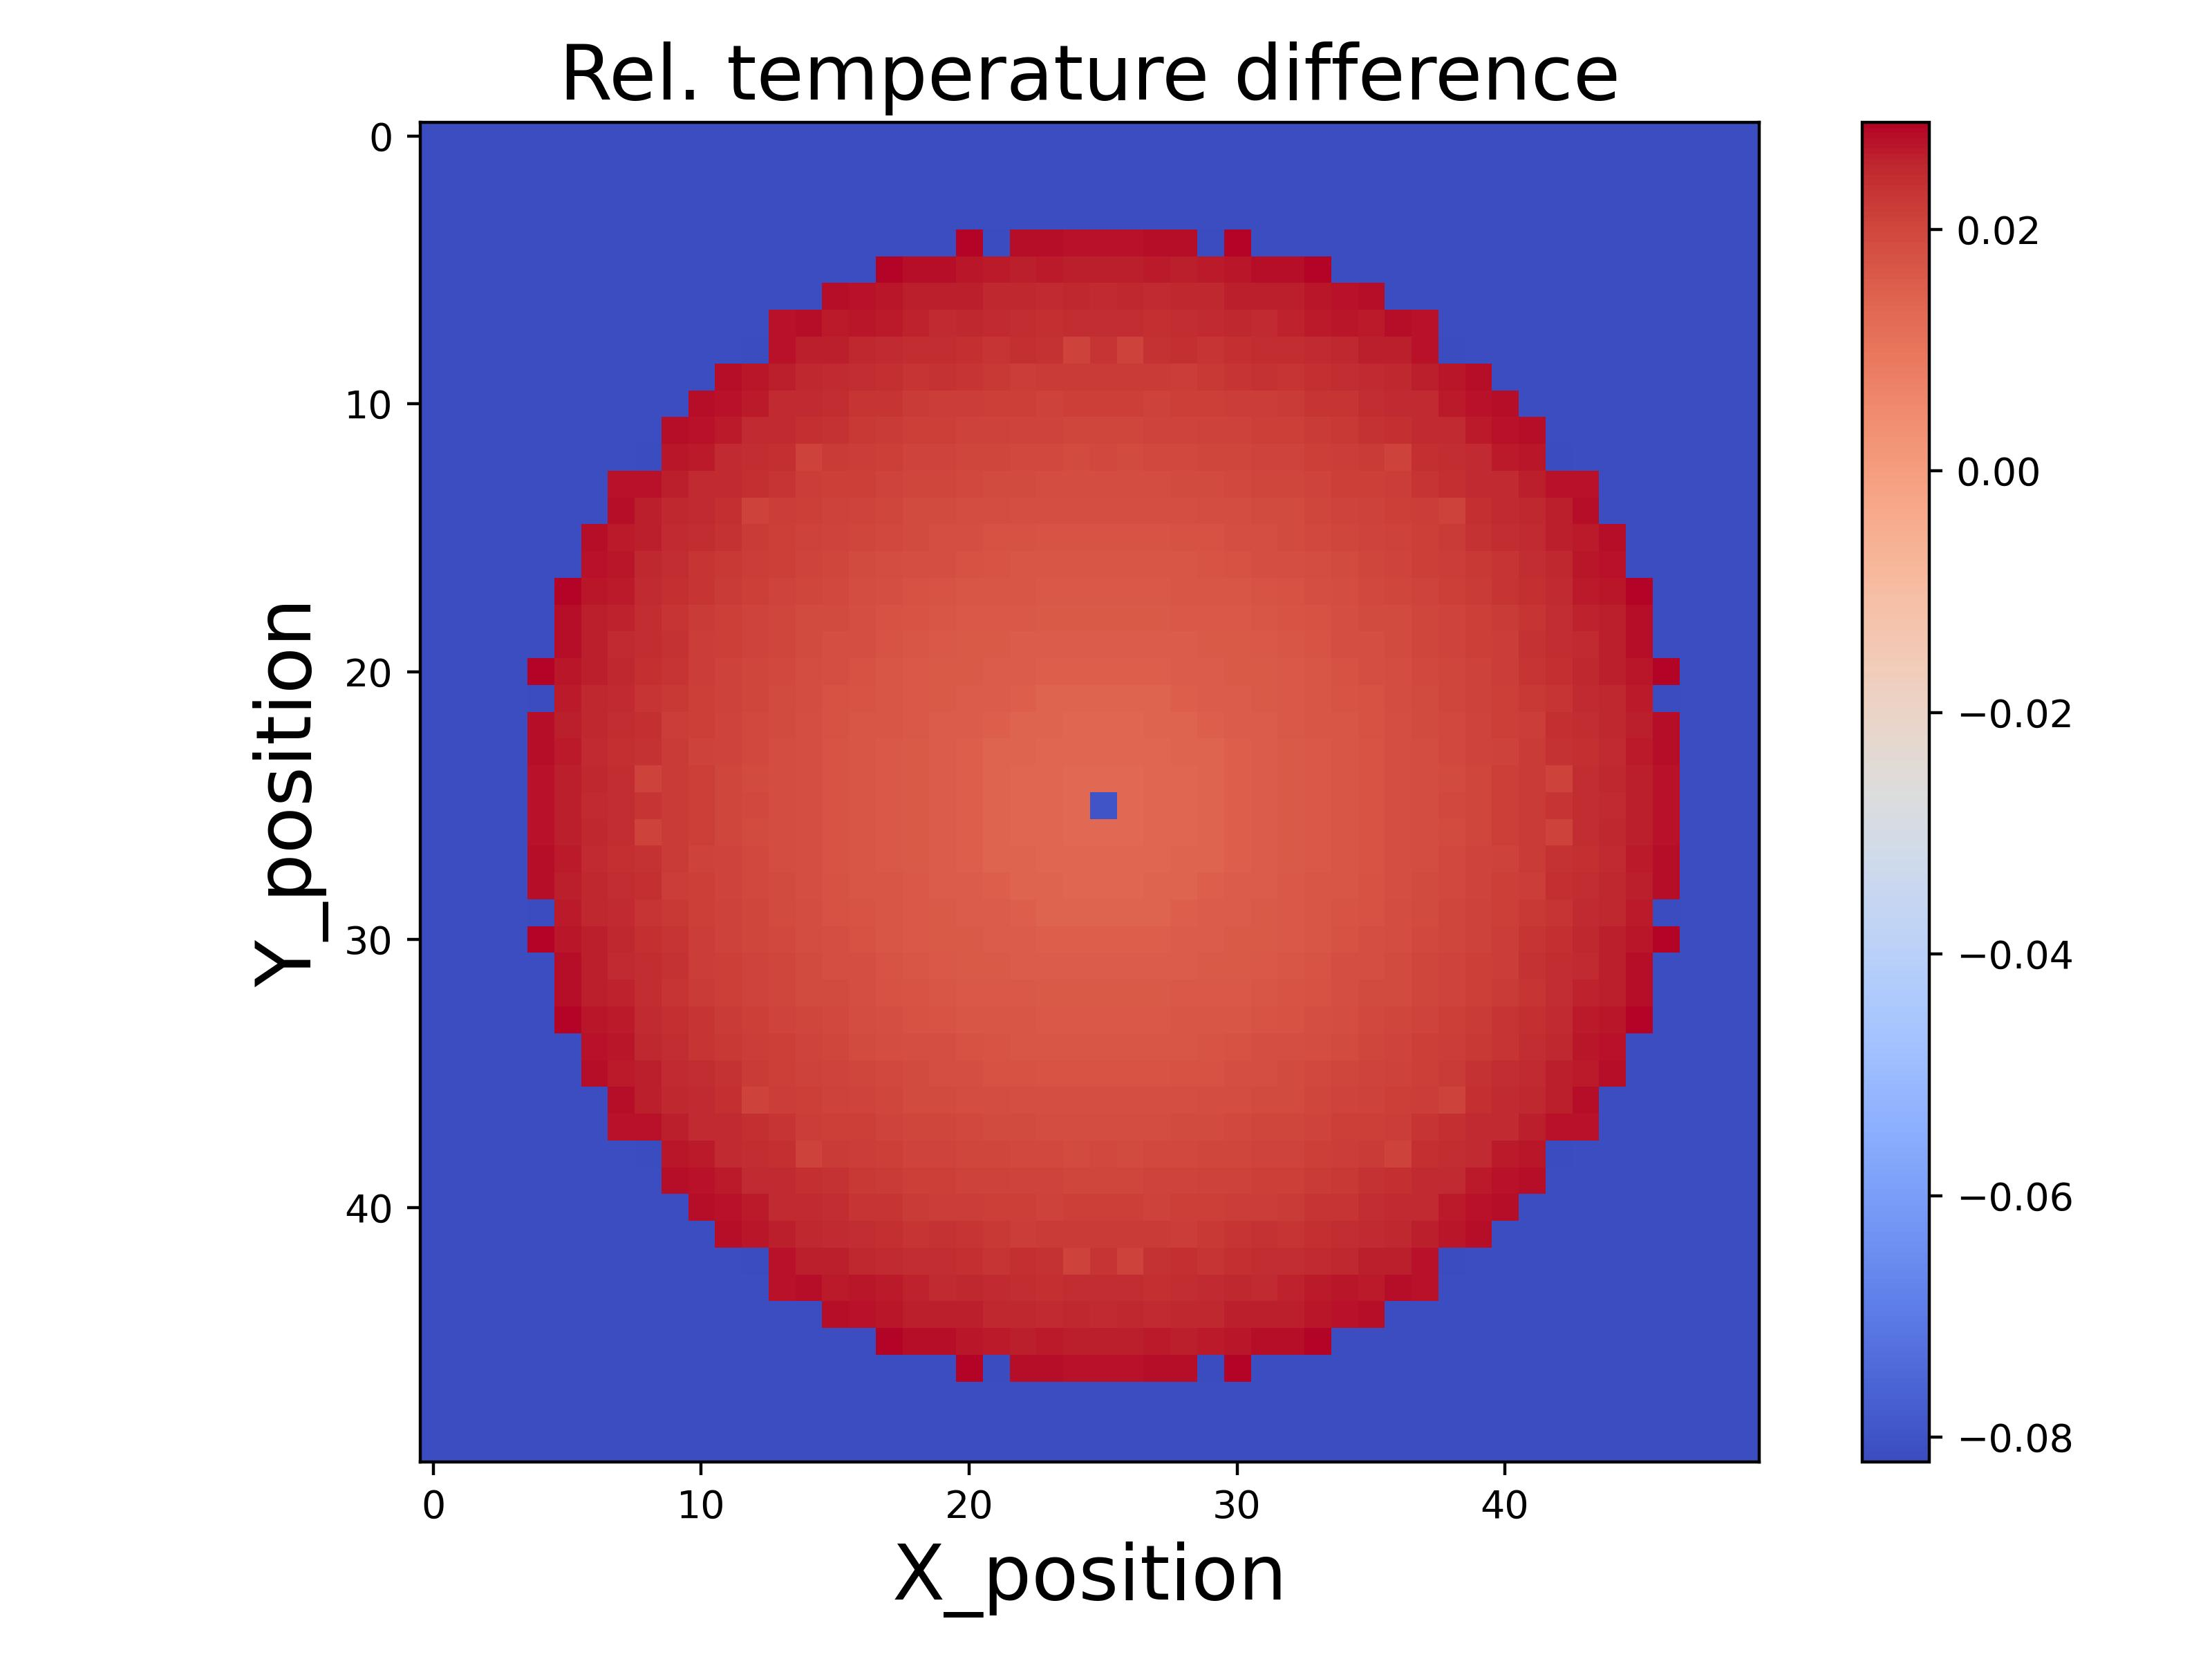
\includegraphics[width=\textwidth]{figures/raw_data/5/lin_square/T_bias.jpg}
            \subcaption{Real iron data}
        \end{subfigure}
        \begin{subfigure}{0.27\textwidth}
            \centering
            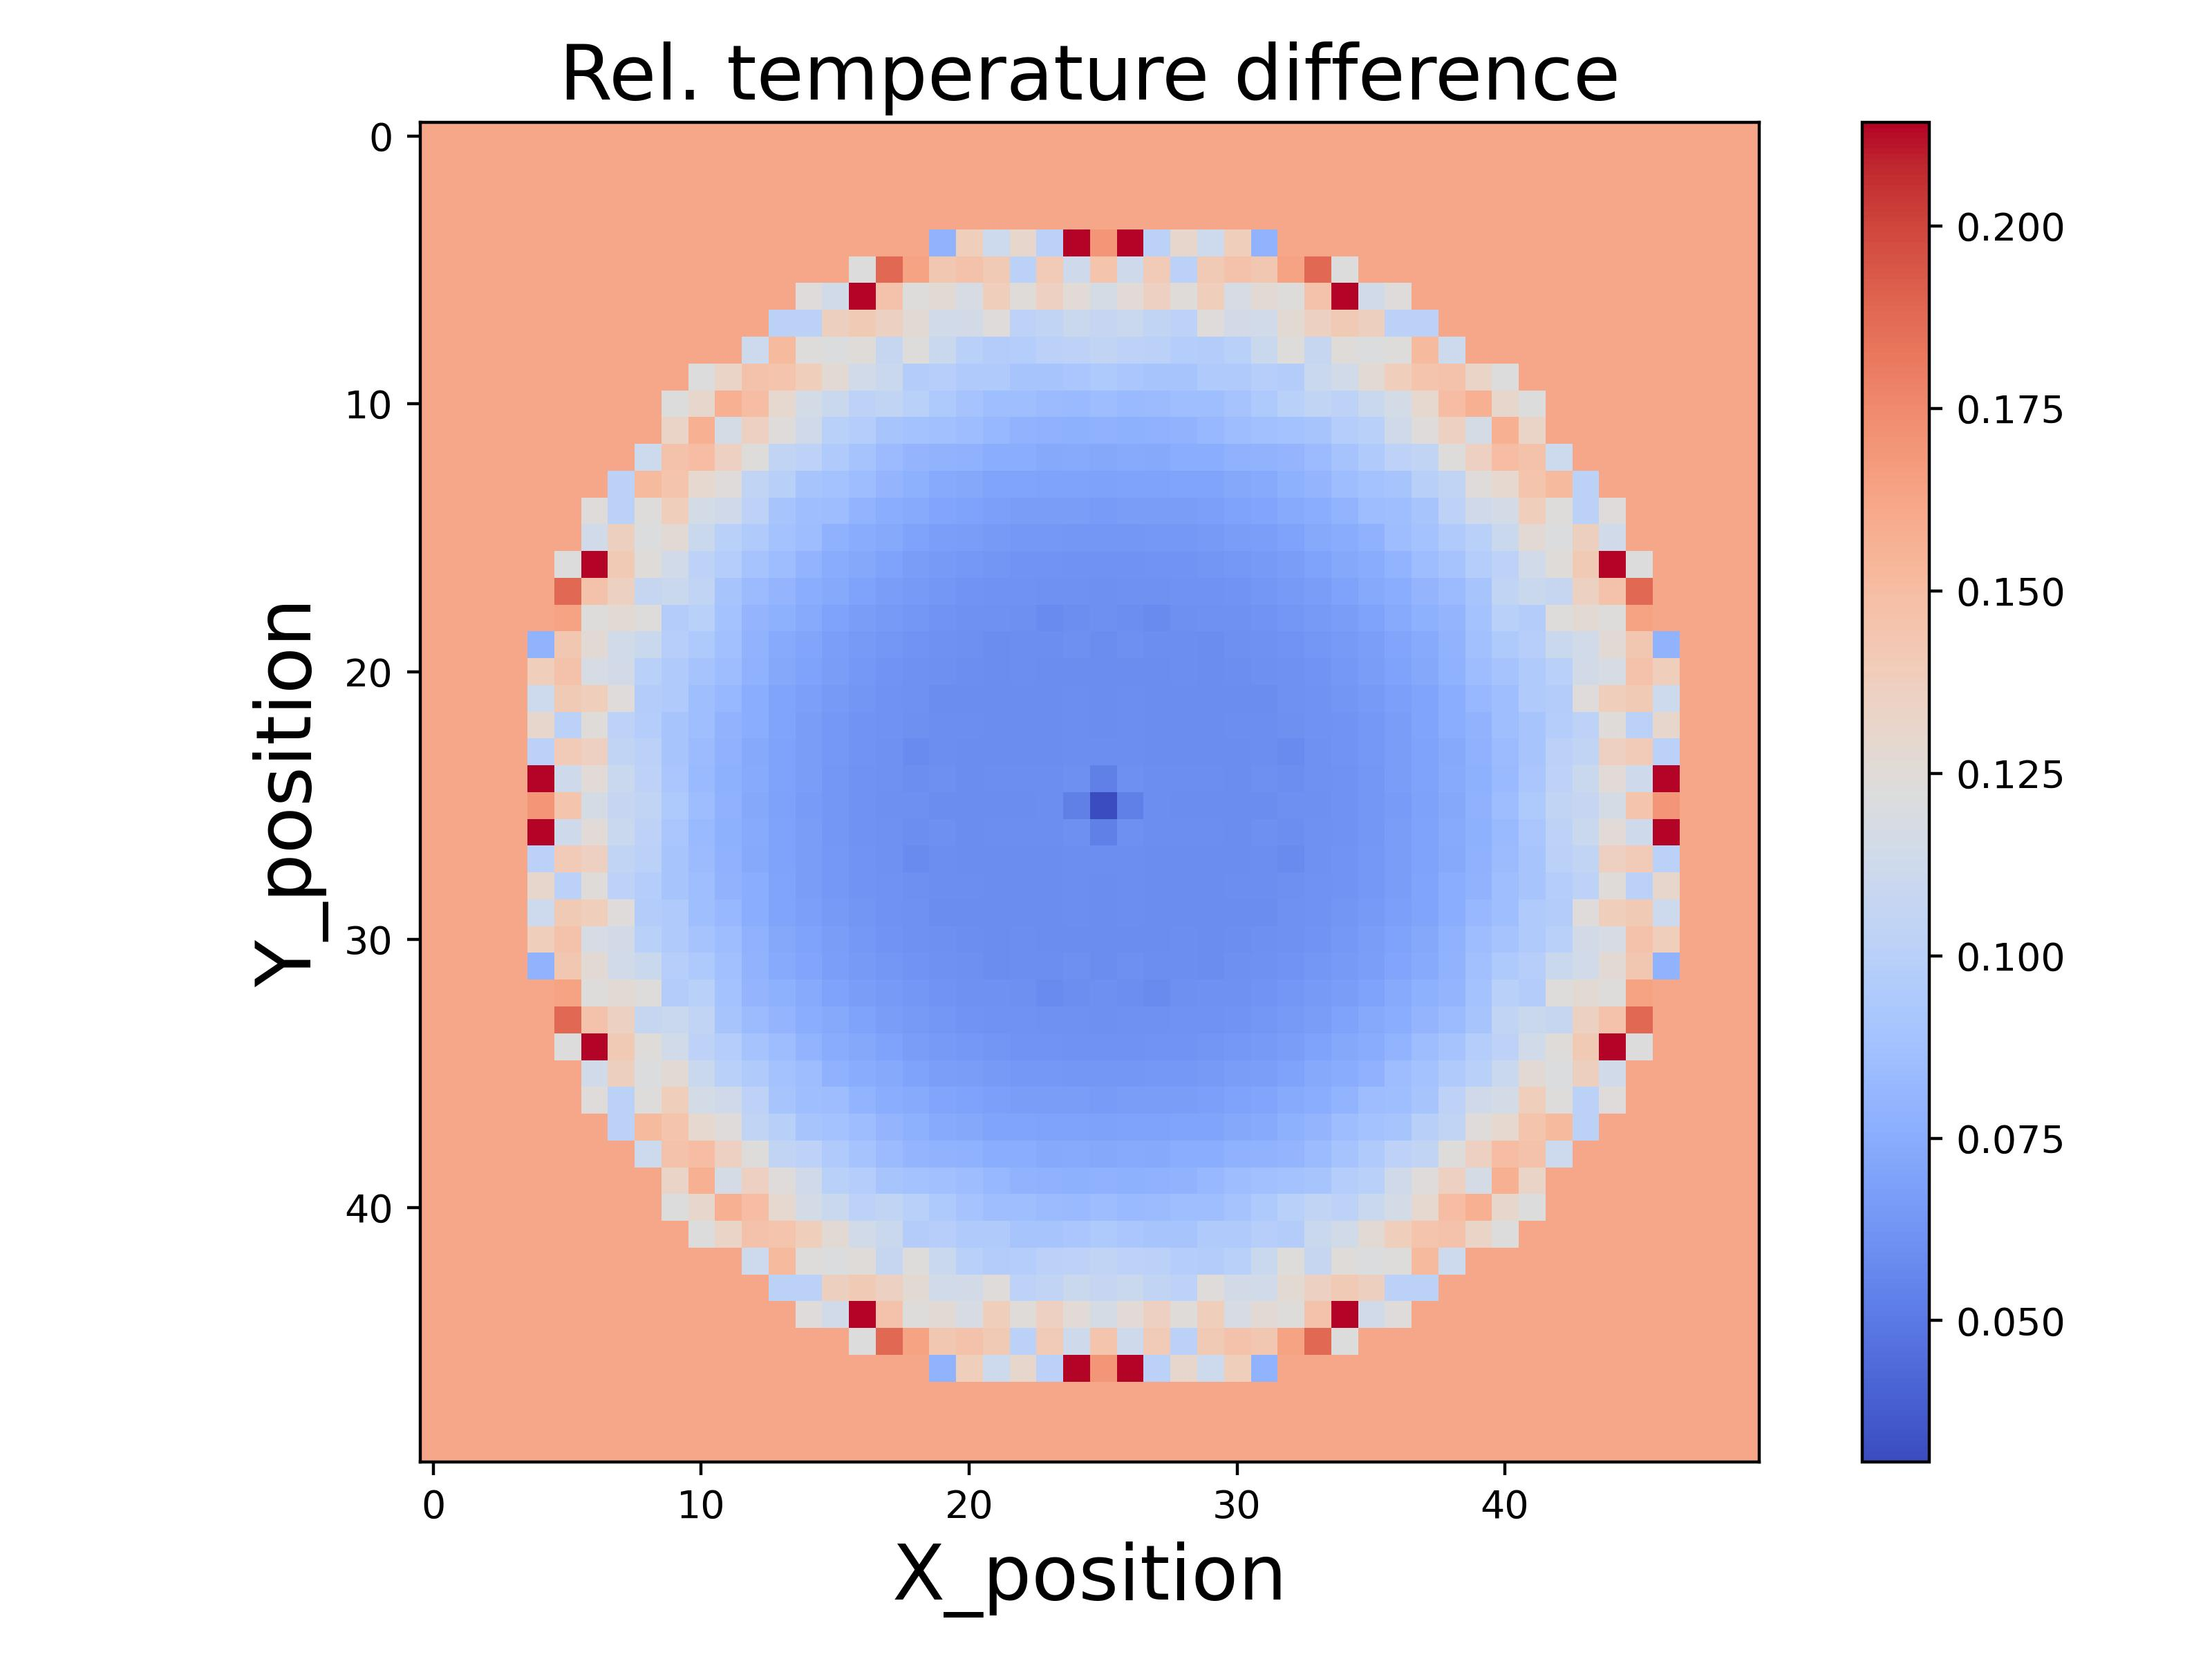
\includegraphics[width=\textwidth]{figures/raw_data/21/lin_square/T_bias.jpg}
            \subcaption{Model 1}
        \end{subfigure}
    \end{minipage}\\
    \begin{minipage}{\textwidth}
        \centering
        \begin{subfigure}{0.27\textwidth}
            \centering
            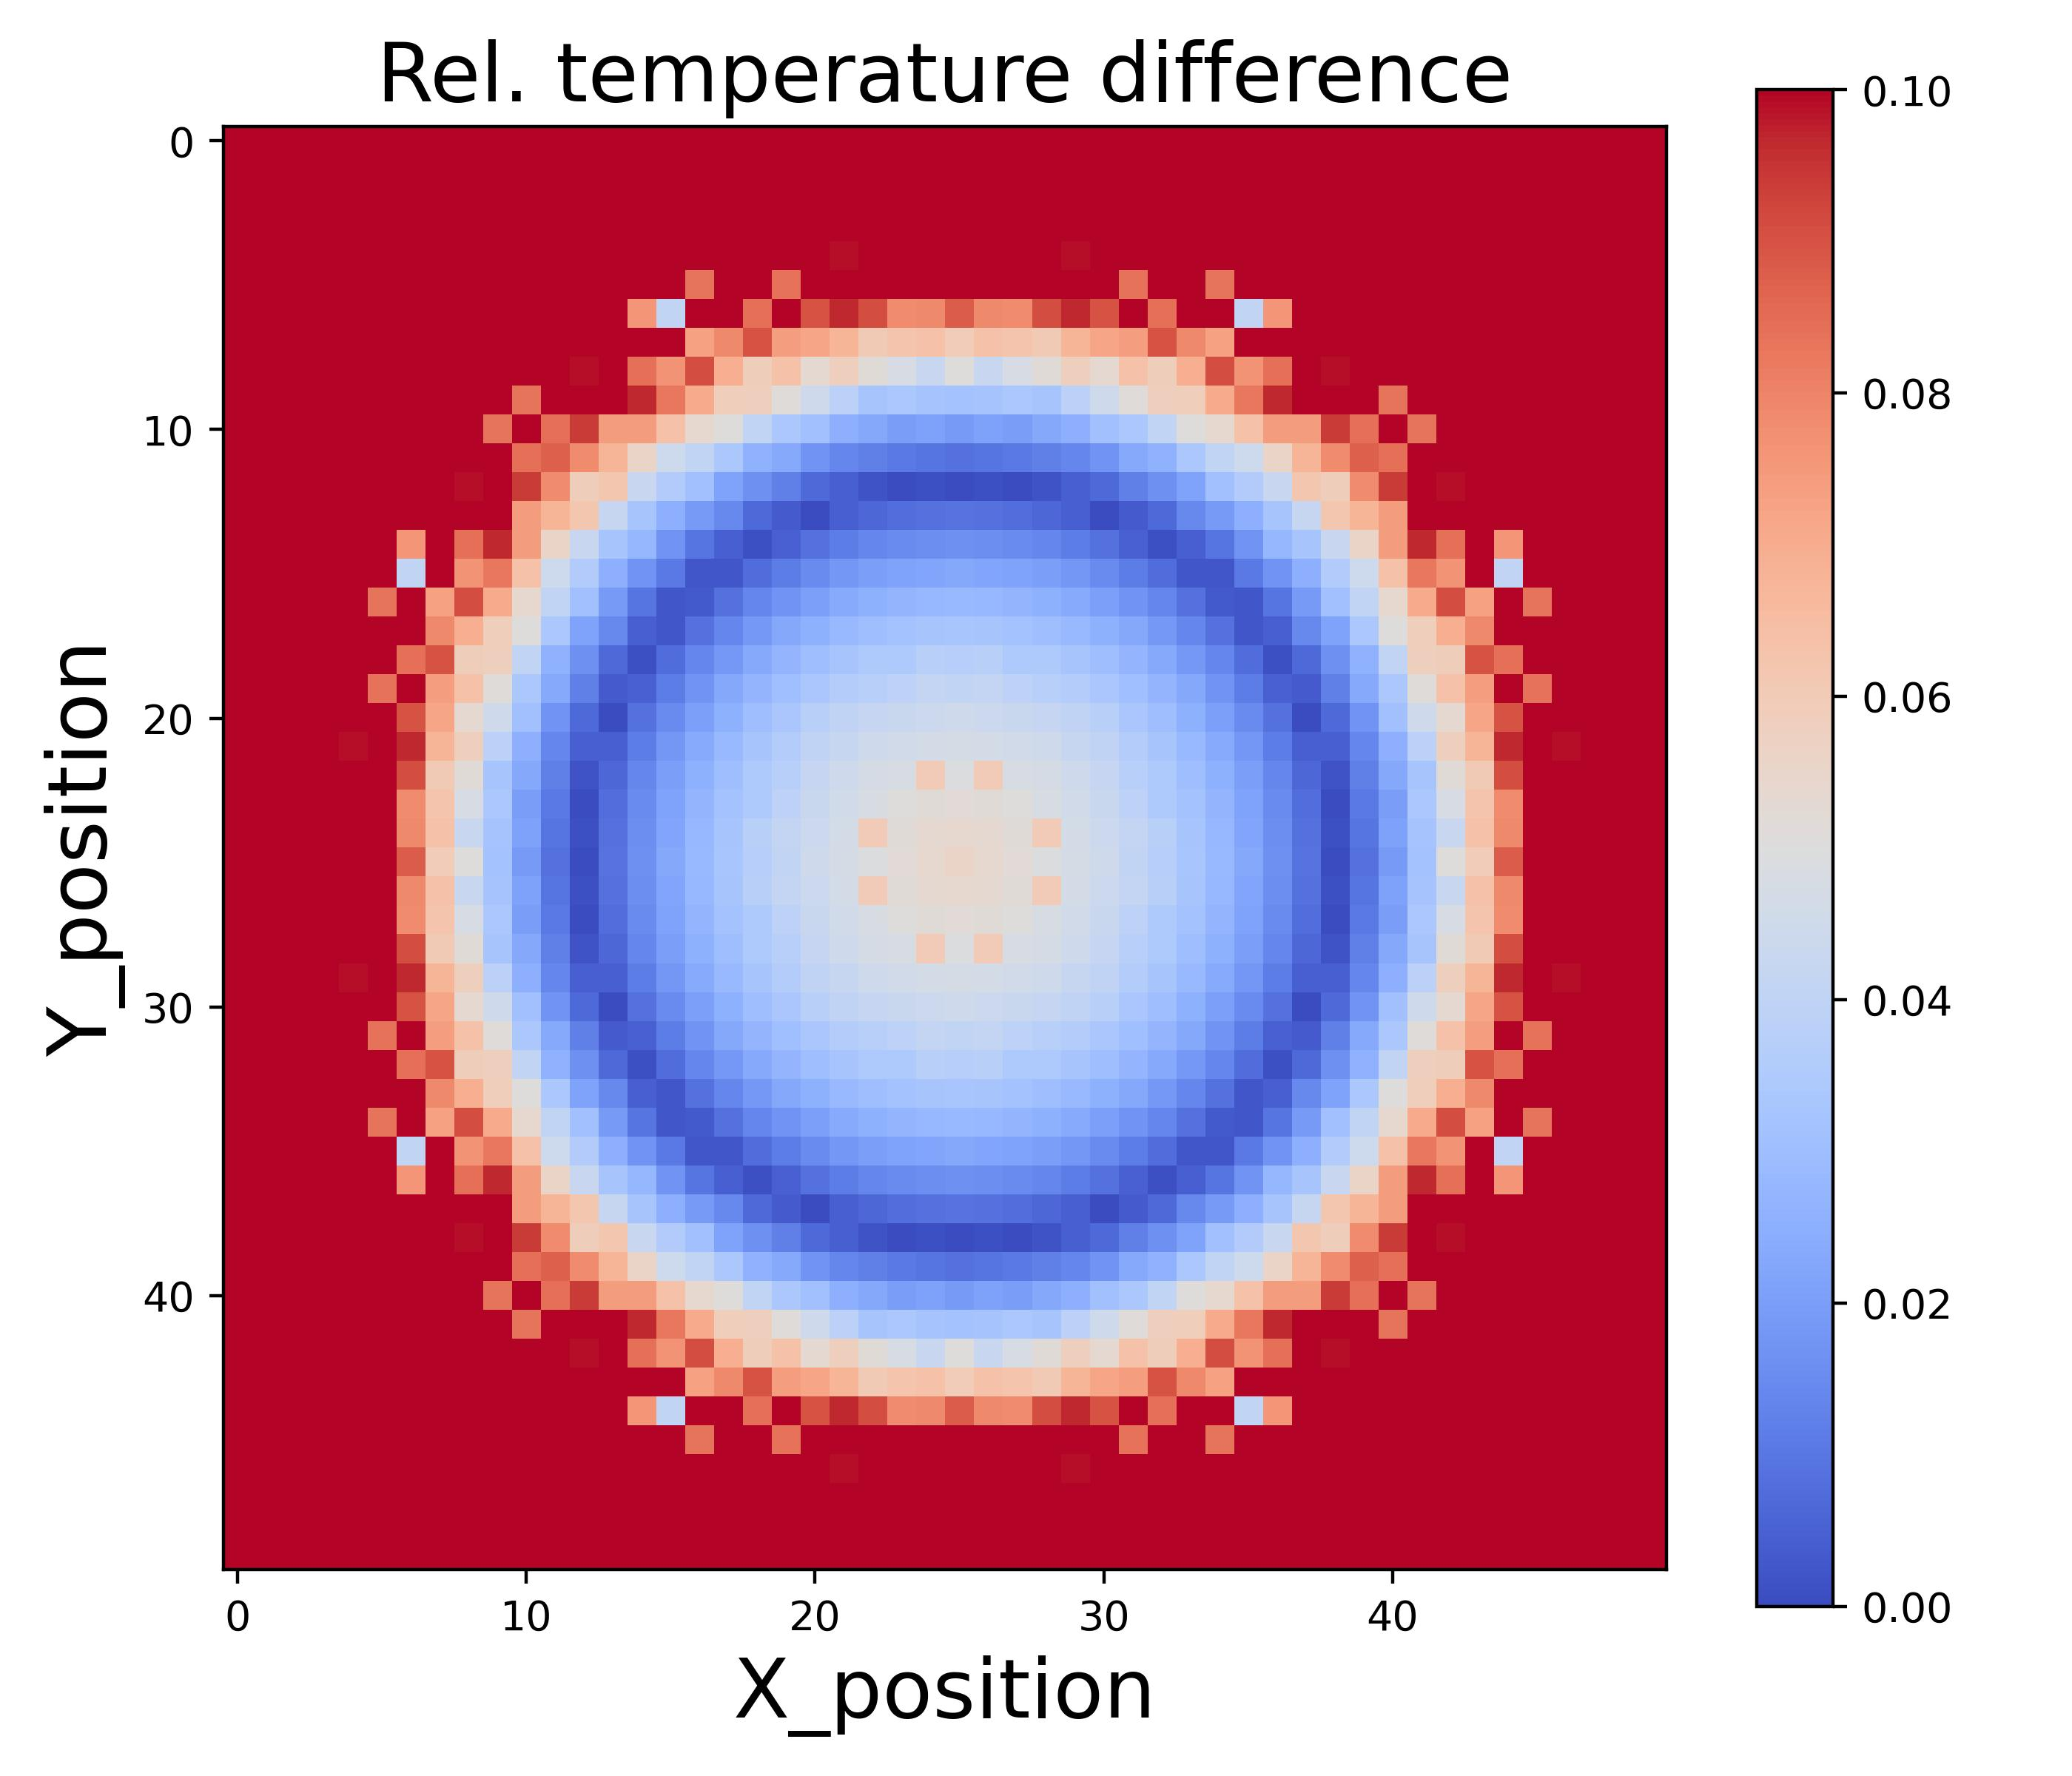
\includegraphics[width=\textwidth]{figures/raw_data/22/lin_square/T_bias.jpg}
            \subcaption{Model 2}
        \end{subfigure}
        \begin{subfigure}{0.27\textwidth}
            \centering
            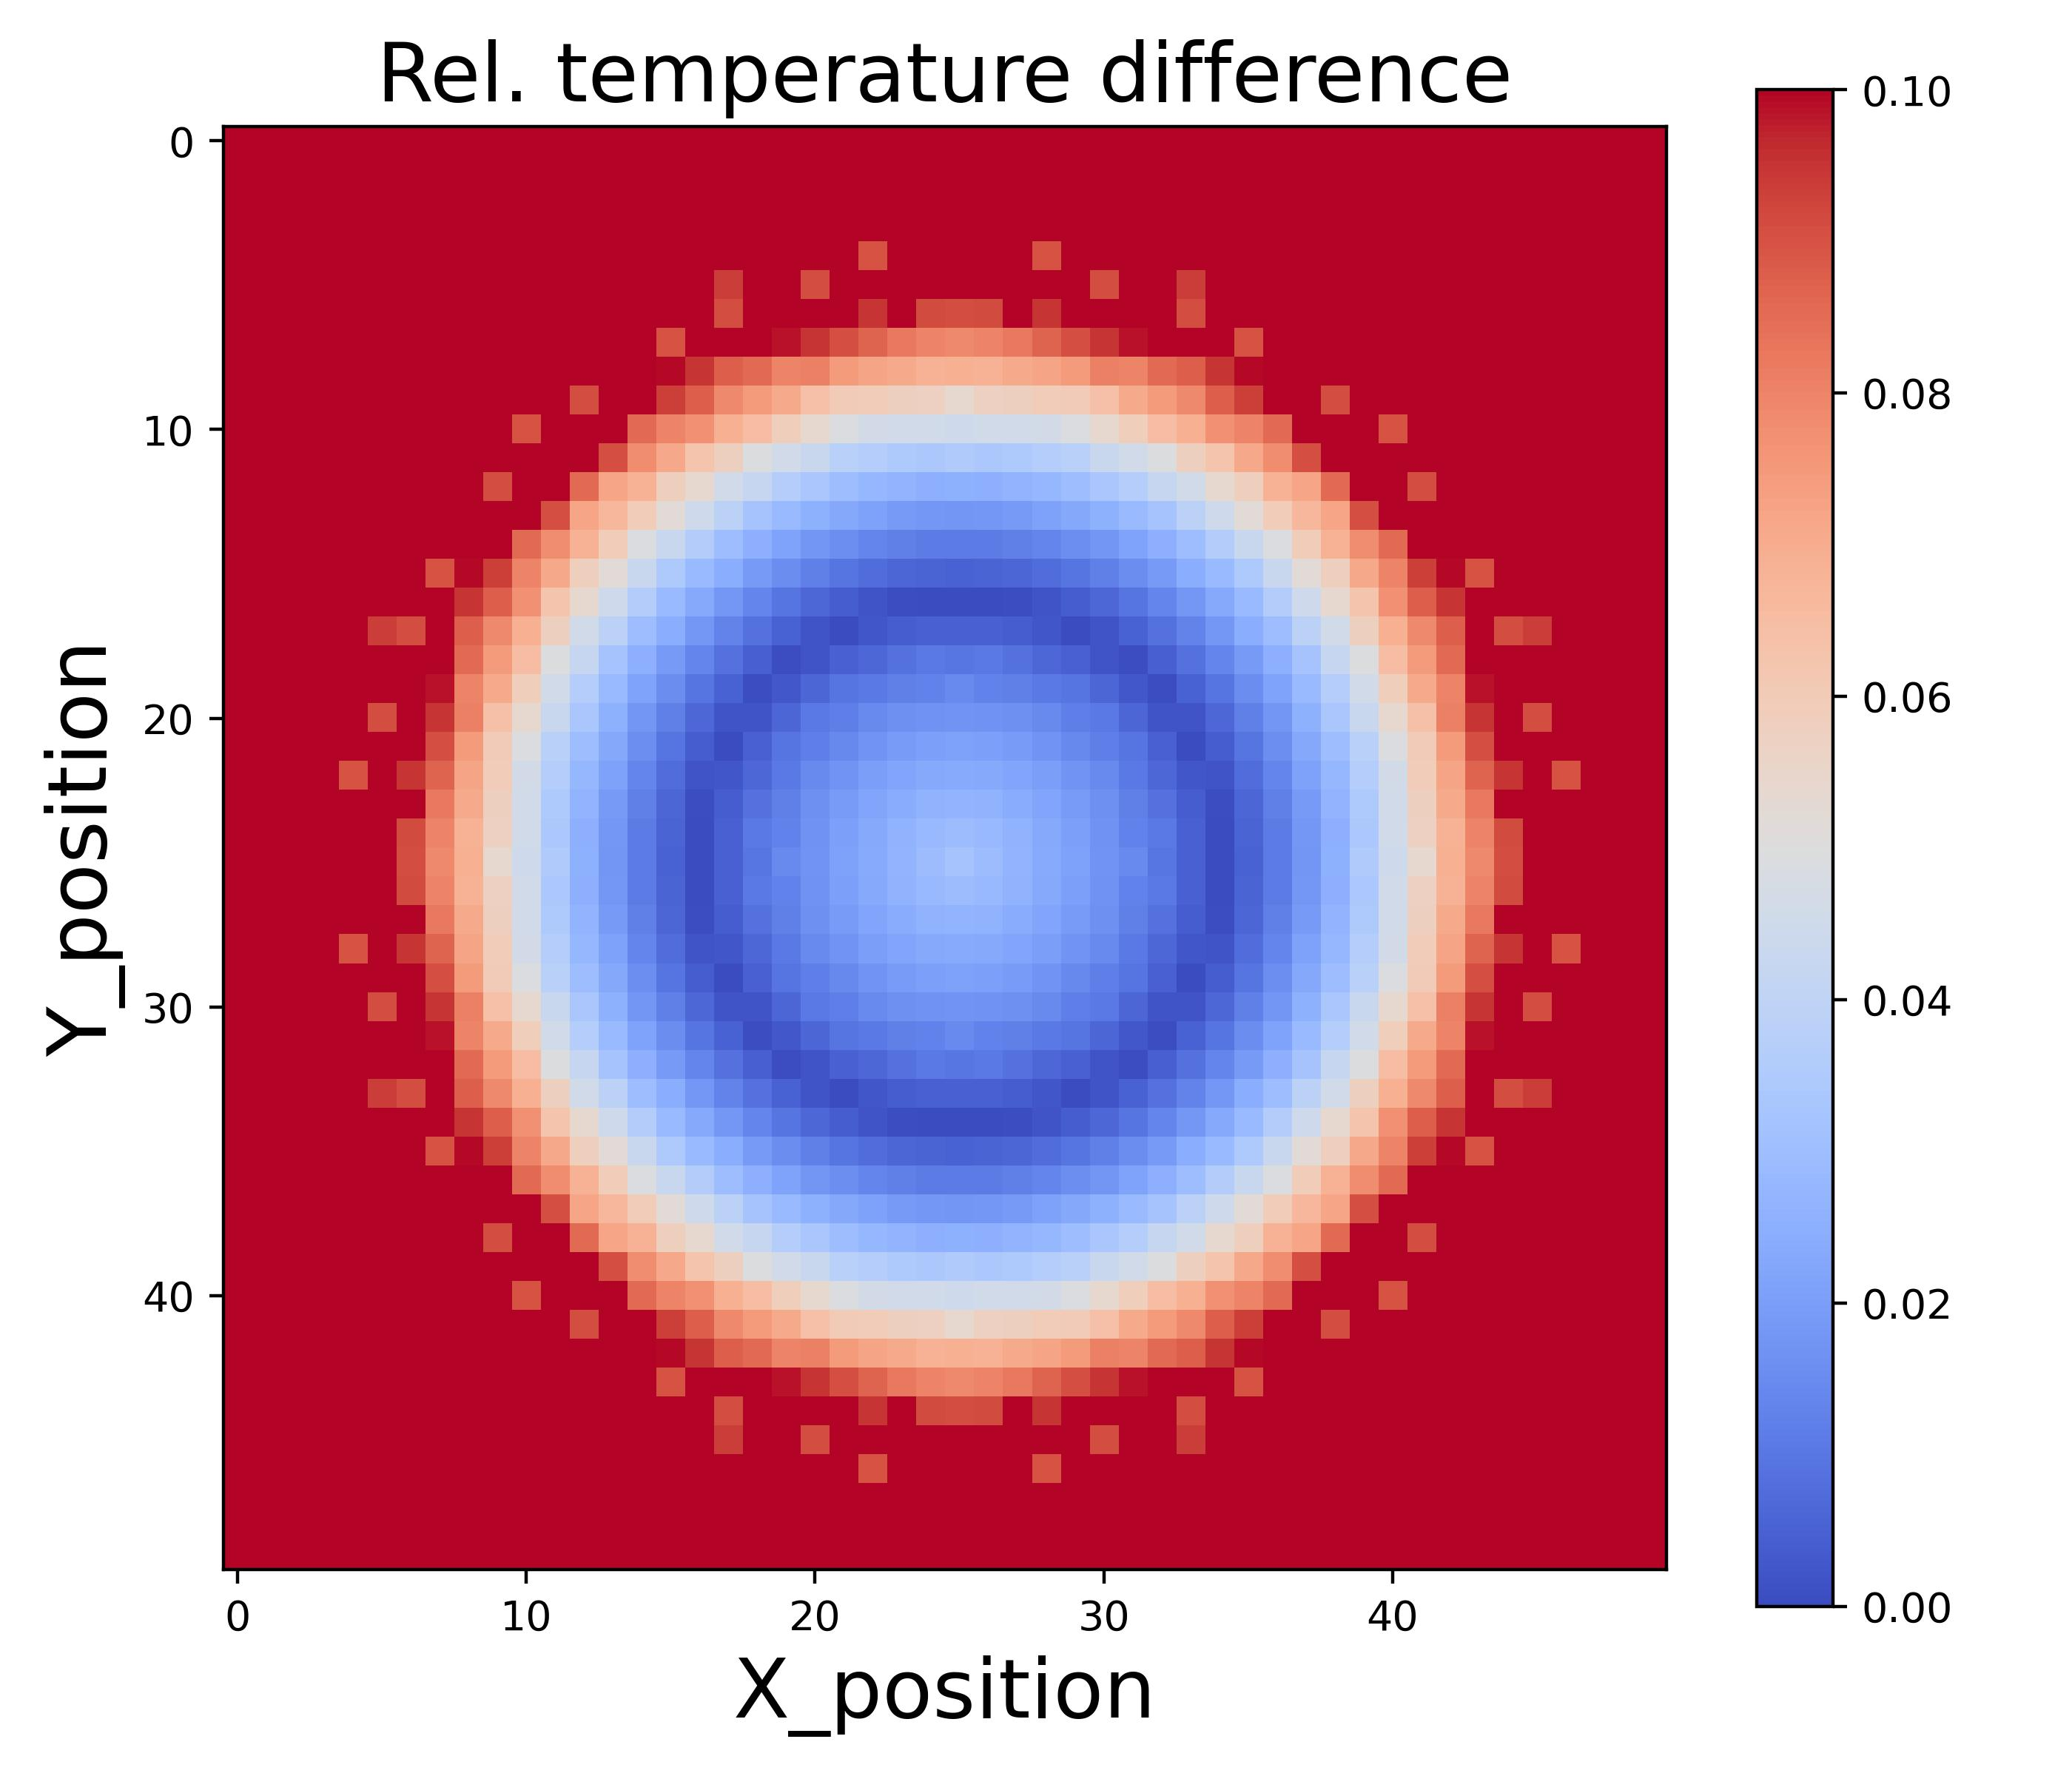
\includegraphics[width=\textwidth]{figures/raw_data/23/lin_square/T_bias.jpg}
            \subcaption{Model 3}
        \end{subfigure}
        \begin{subfigure}{0.27\textwidth}
            \centering
            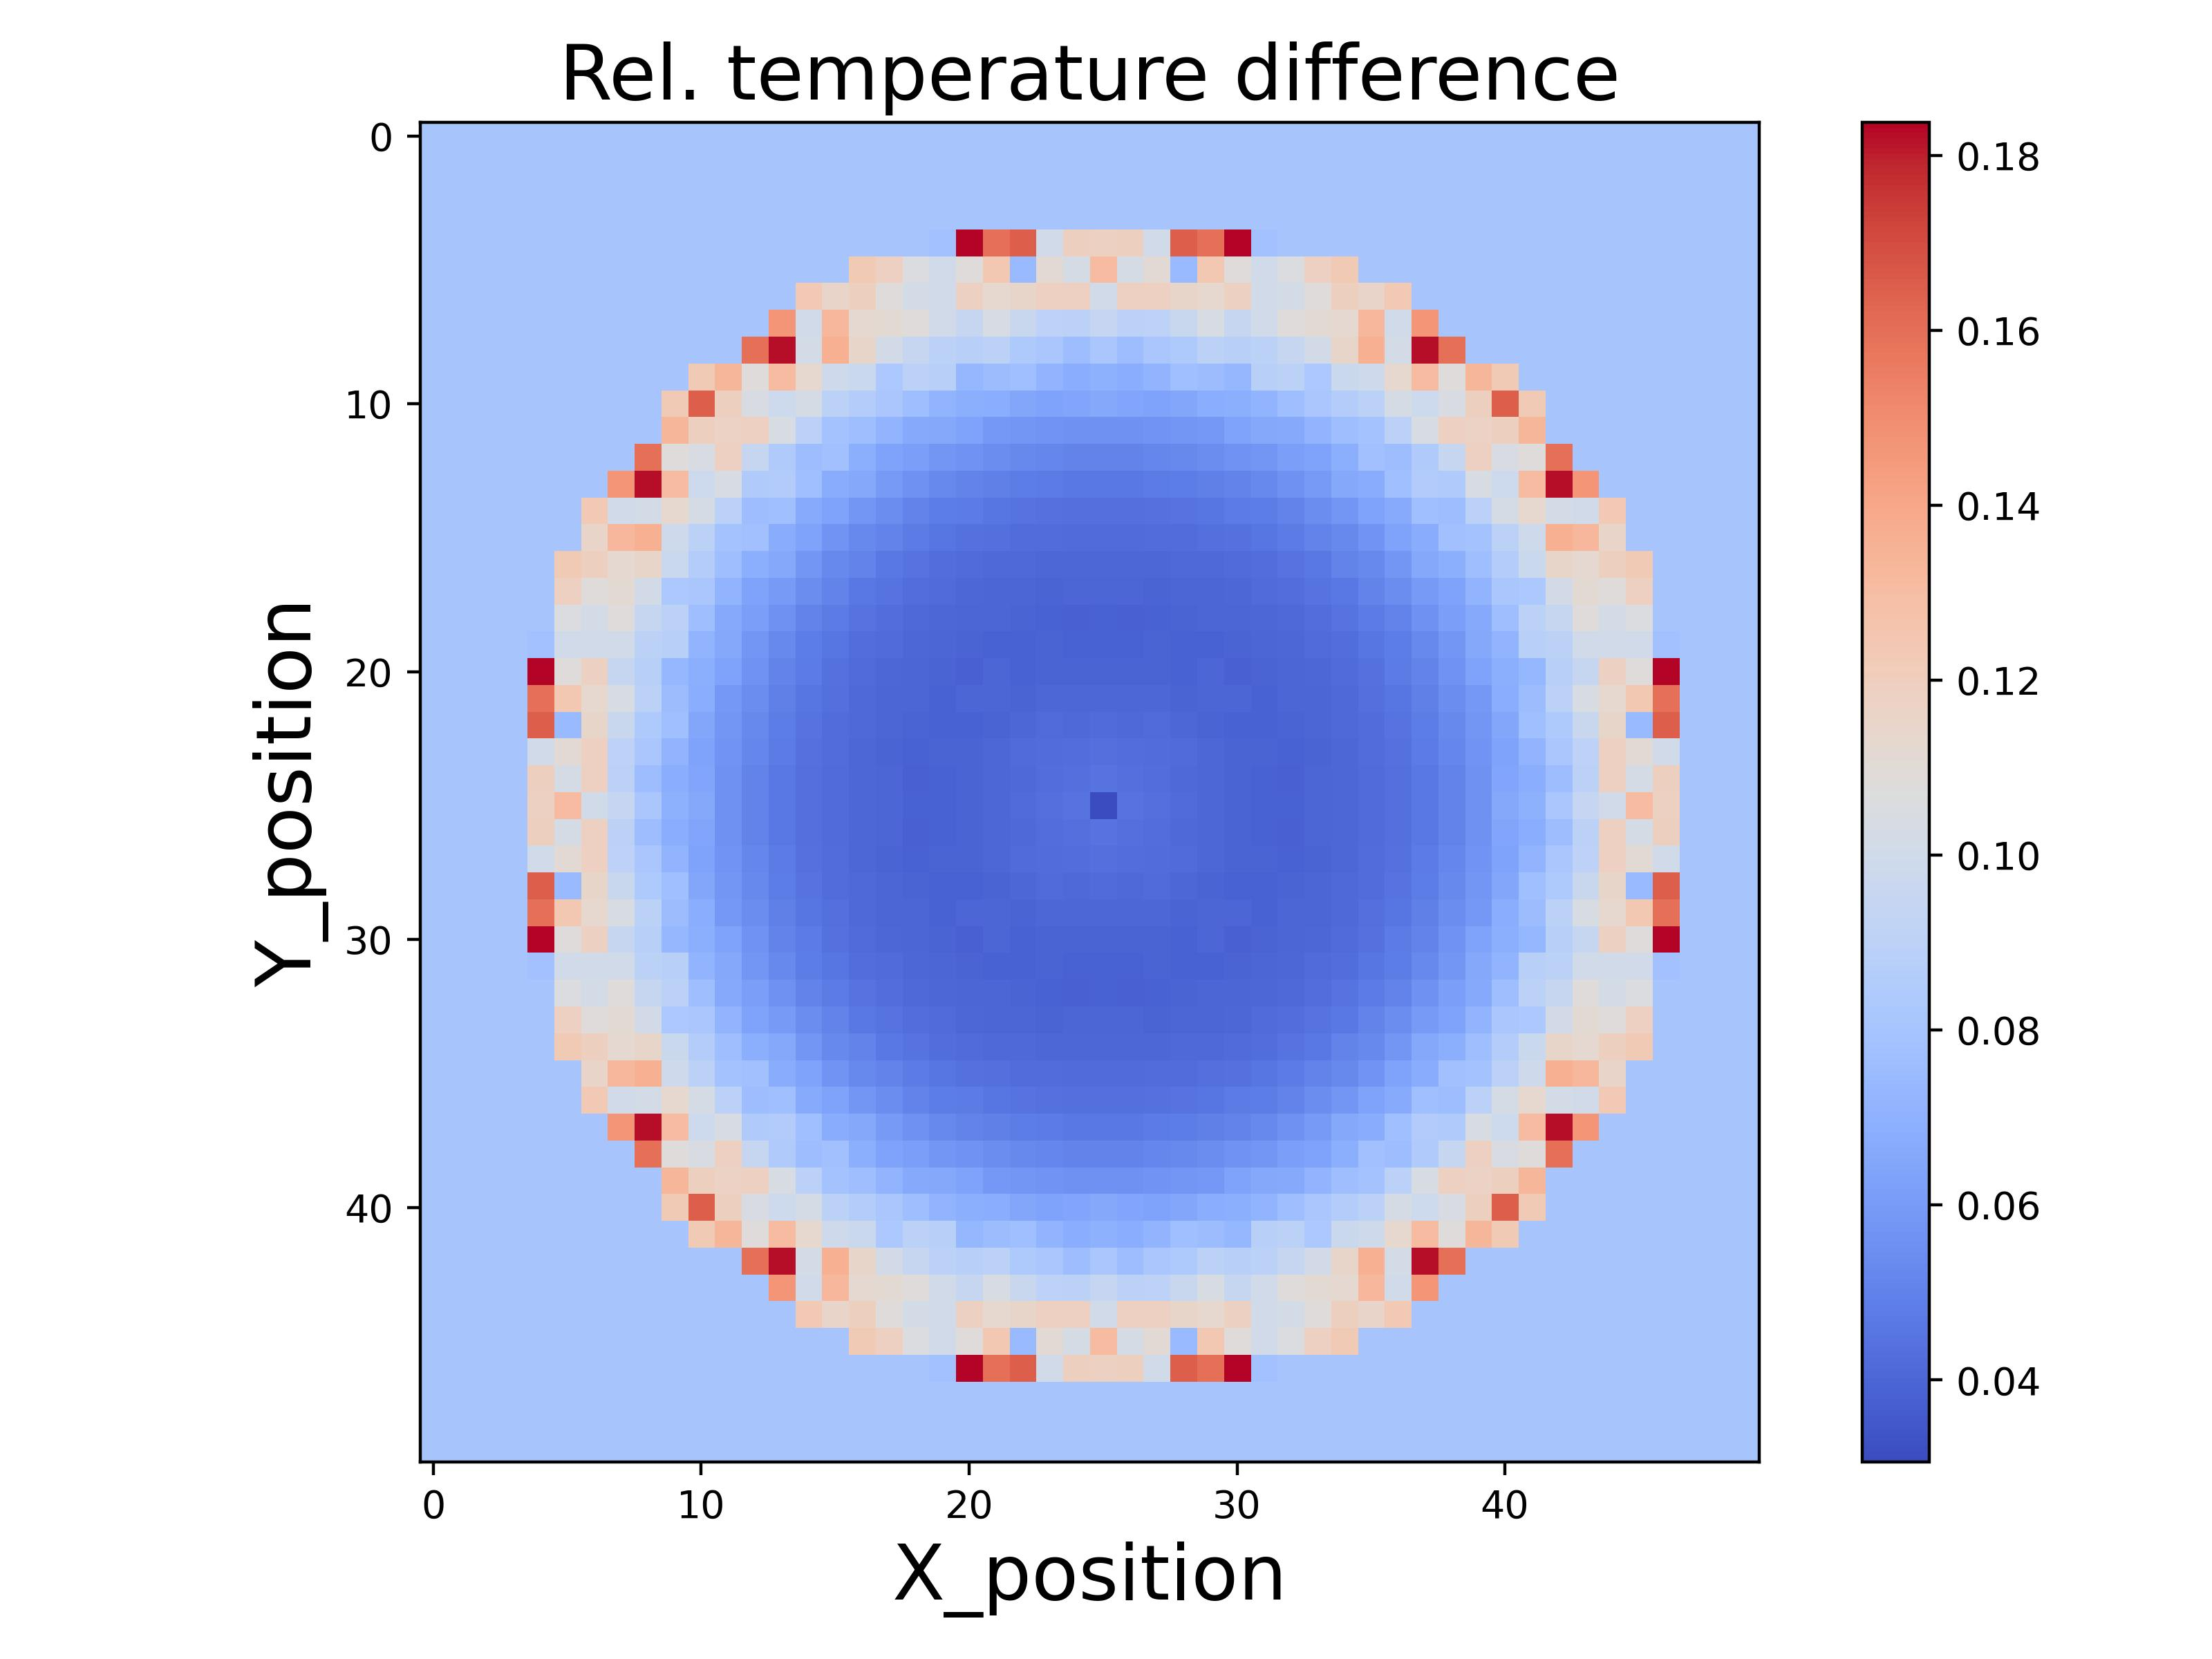
\includegraphics[width=\textwidth]{figures/raw_data/24/lin_square/T_bias.jpg}
            \subcaption{Model 4}
        \end{subfigure}
    \end{minipage}\\
    \begin{minipage}{\textwidth}
        \centering
        \begin{subfigure}{0.27\textwidth}
            \centering
            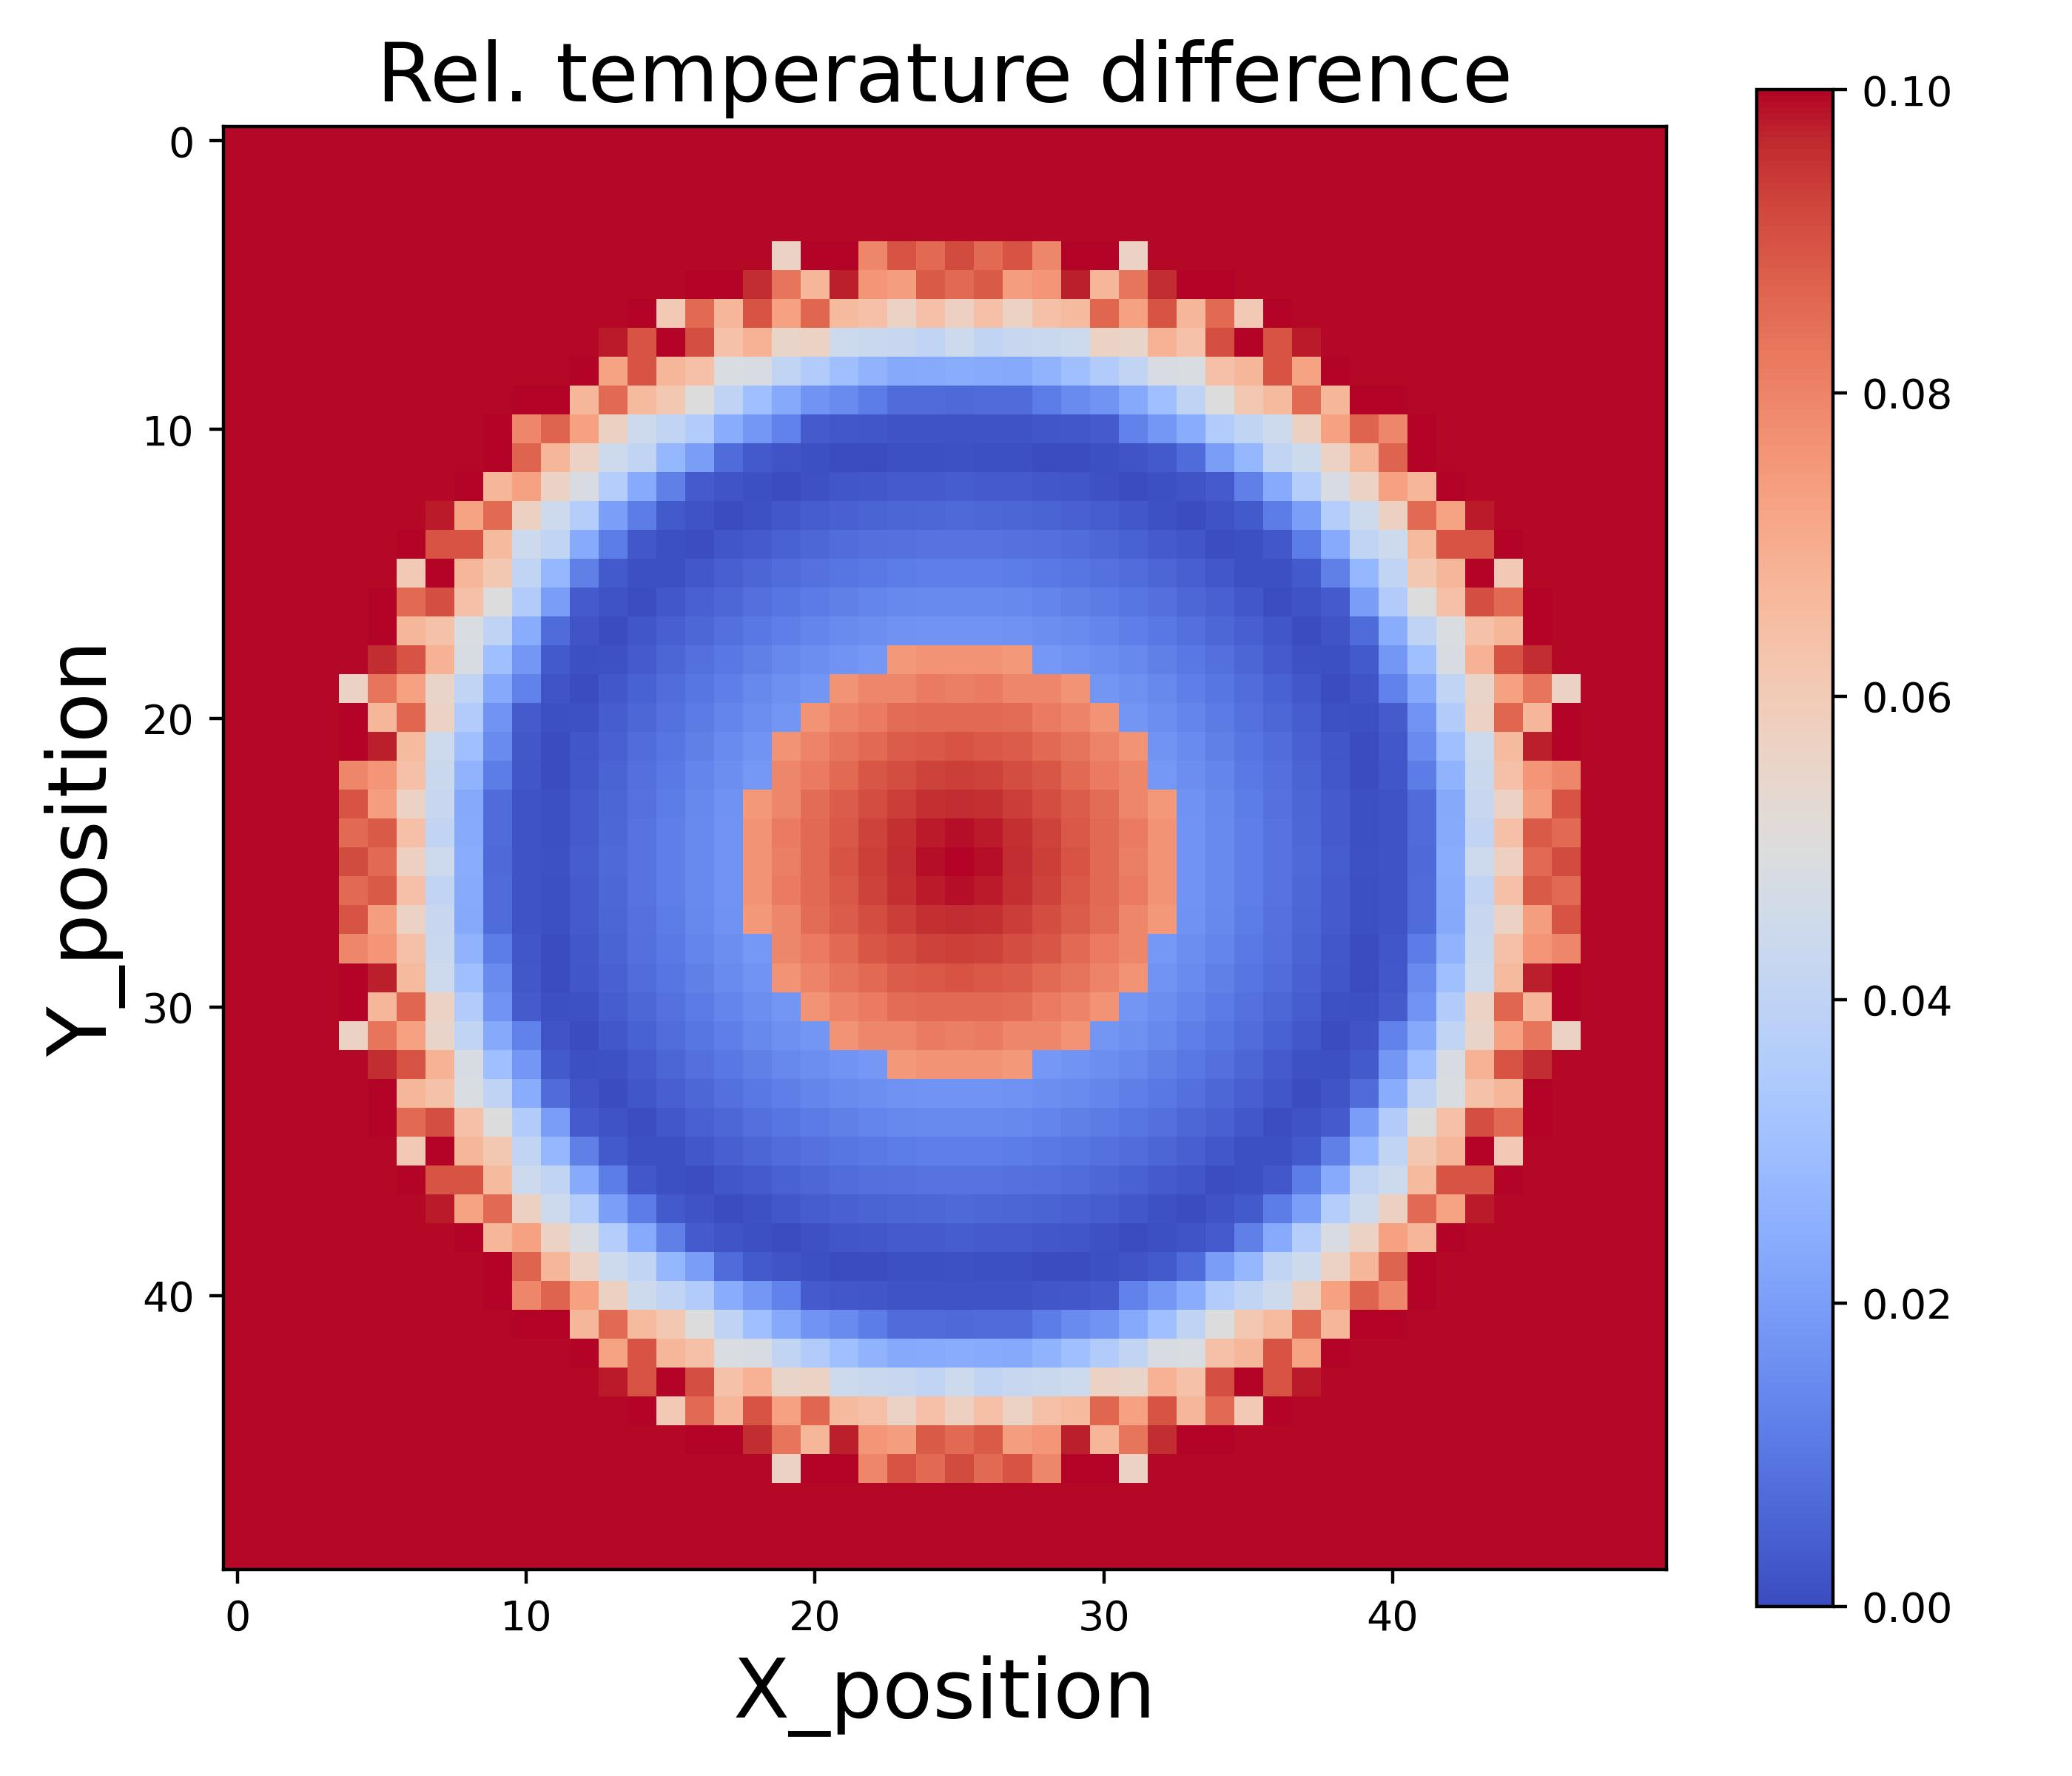
\includegraphics[width=\textwidth]{figures/raw_data/25/lin_square/T_bias.jpg}
            \subcaption{Model 5}
        \end{subfigure}
        \begin{subfigure}{0.27\textwidth}
            \centering
            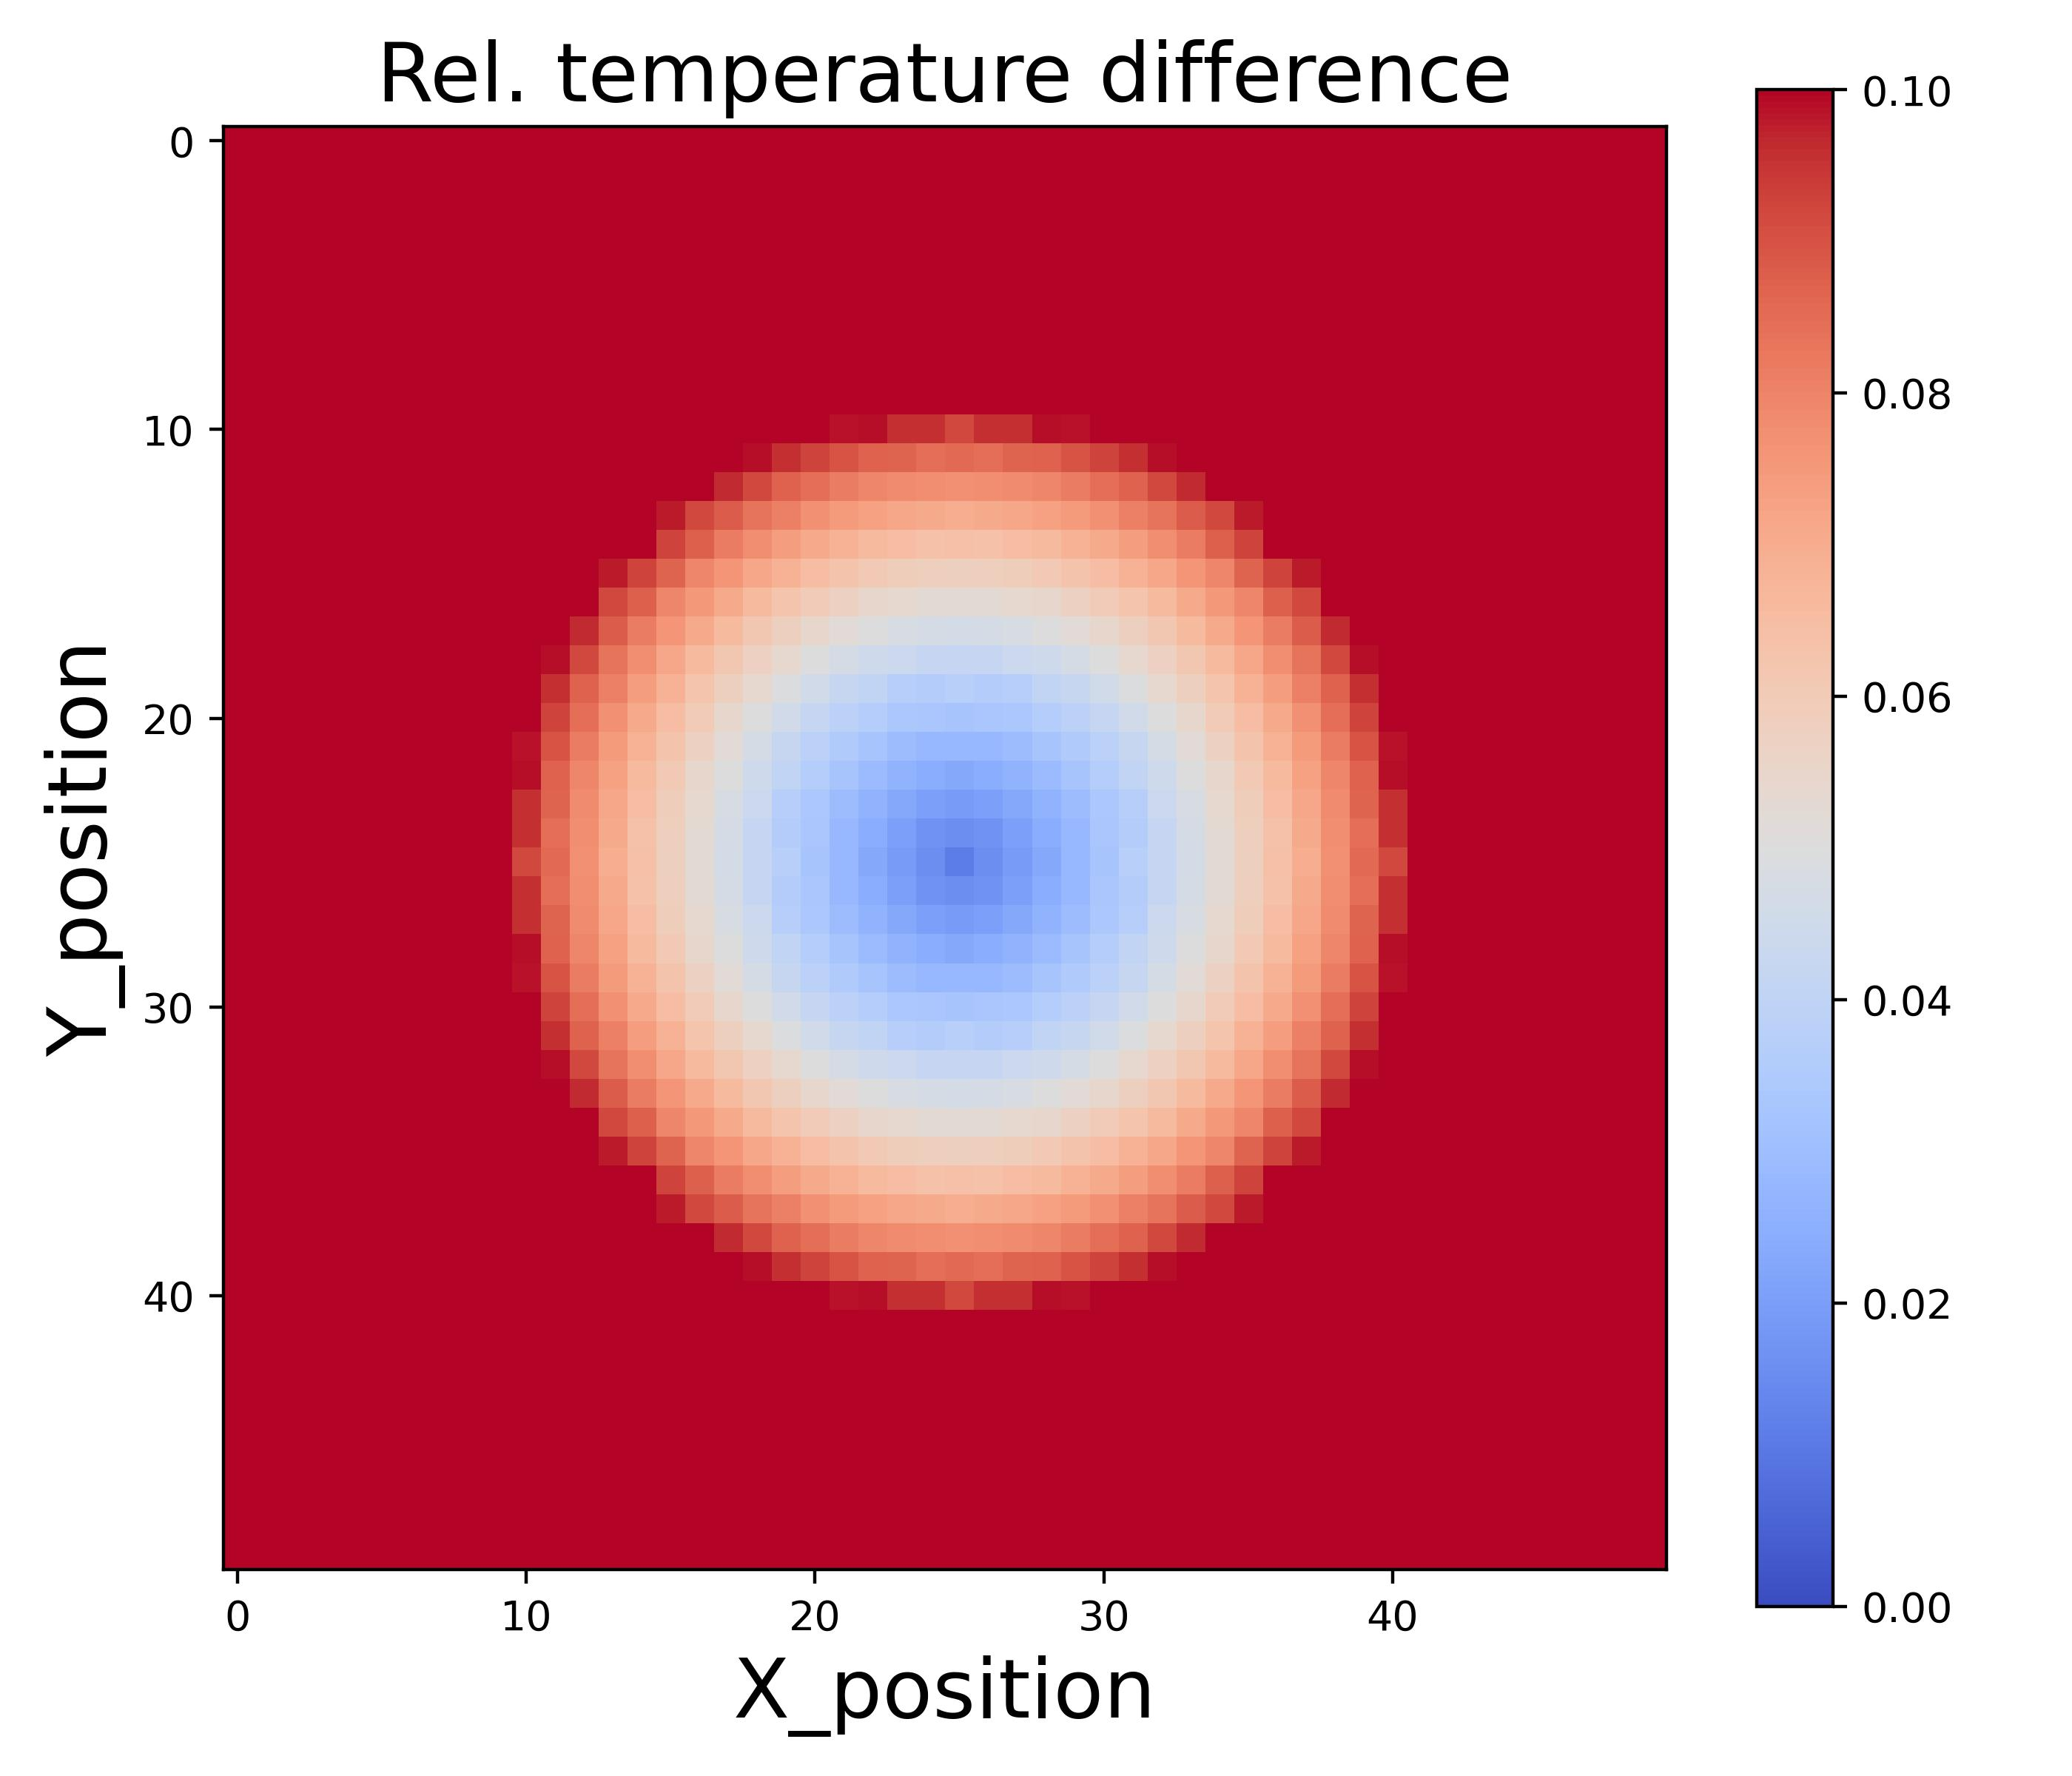
\includegraphics[width=\textwidth]{figures/raw_data/26/lin_square/T_bias.jpg}
            \subcaption{Model 6}
        \end{subfigure}
        \begin{subfigure}{0.27\textwidth}
            \centering
            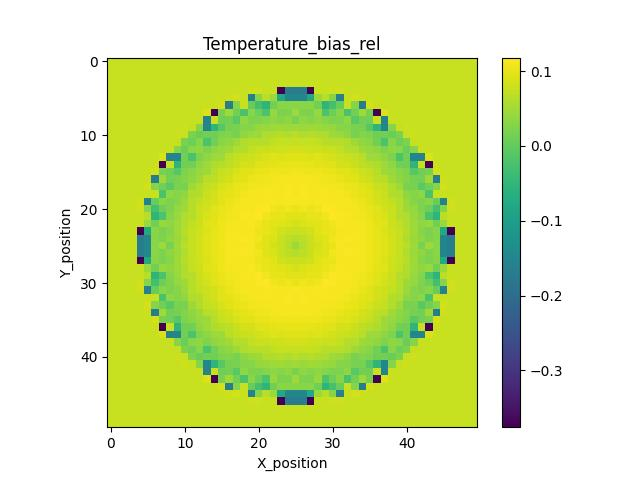
\includegraphics[width=\textwidth]{figures/raw_data/31/lin_square/T_bias.jpg}
            \subcaption{Model 7}
        \end{subfigure}
    \end{minipage}\\
    \begin{minipage}{\textwidth}
        \centering
        \begin{subfigure}{0.27\textwidth}
            \centering
            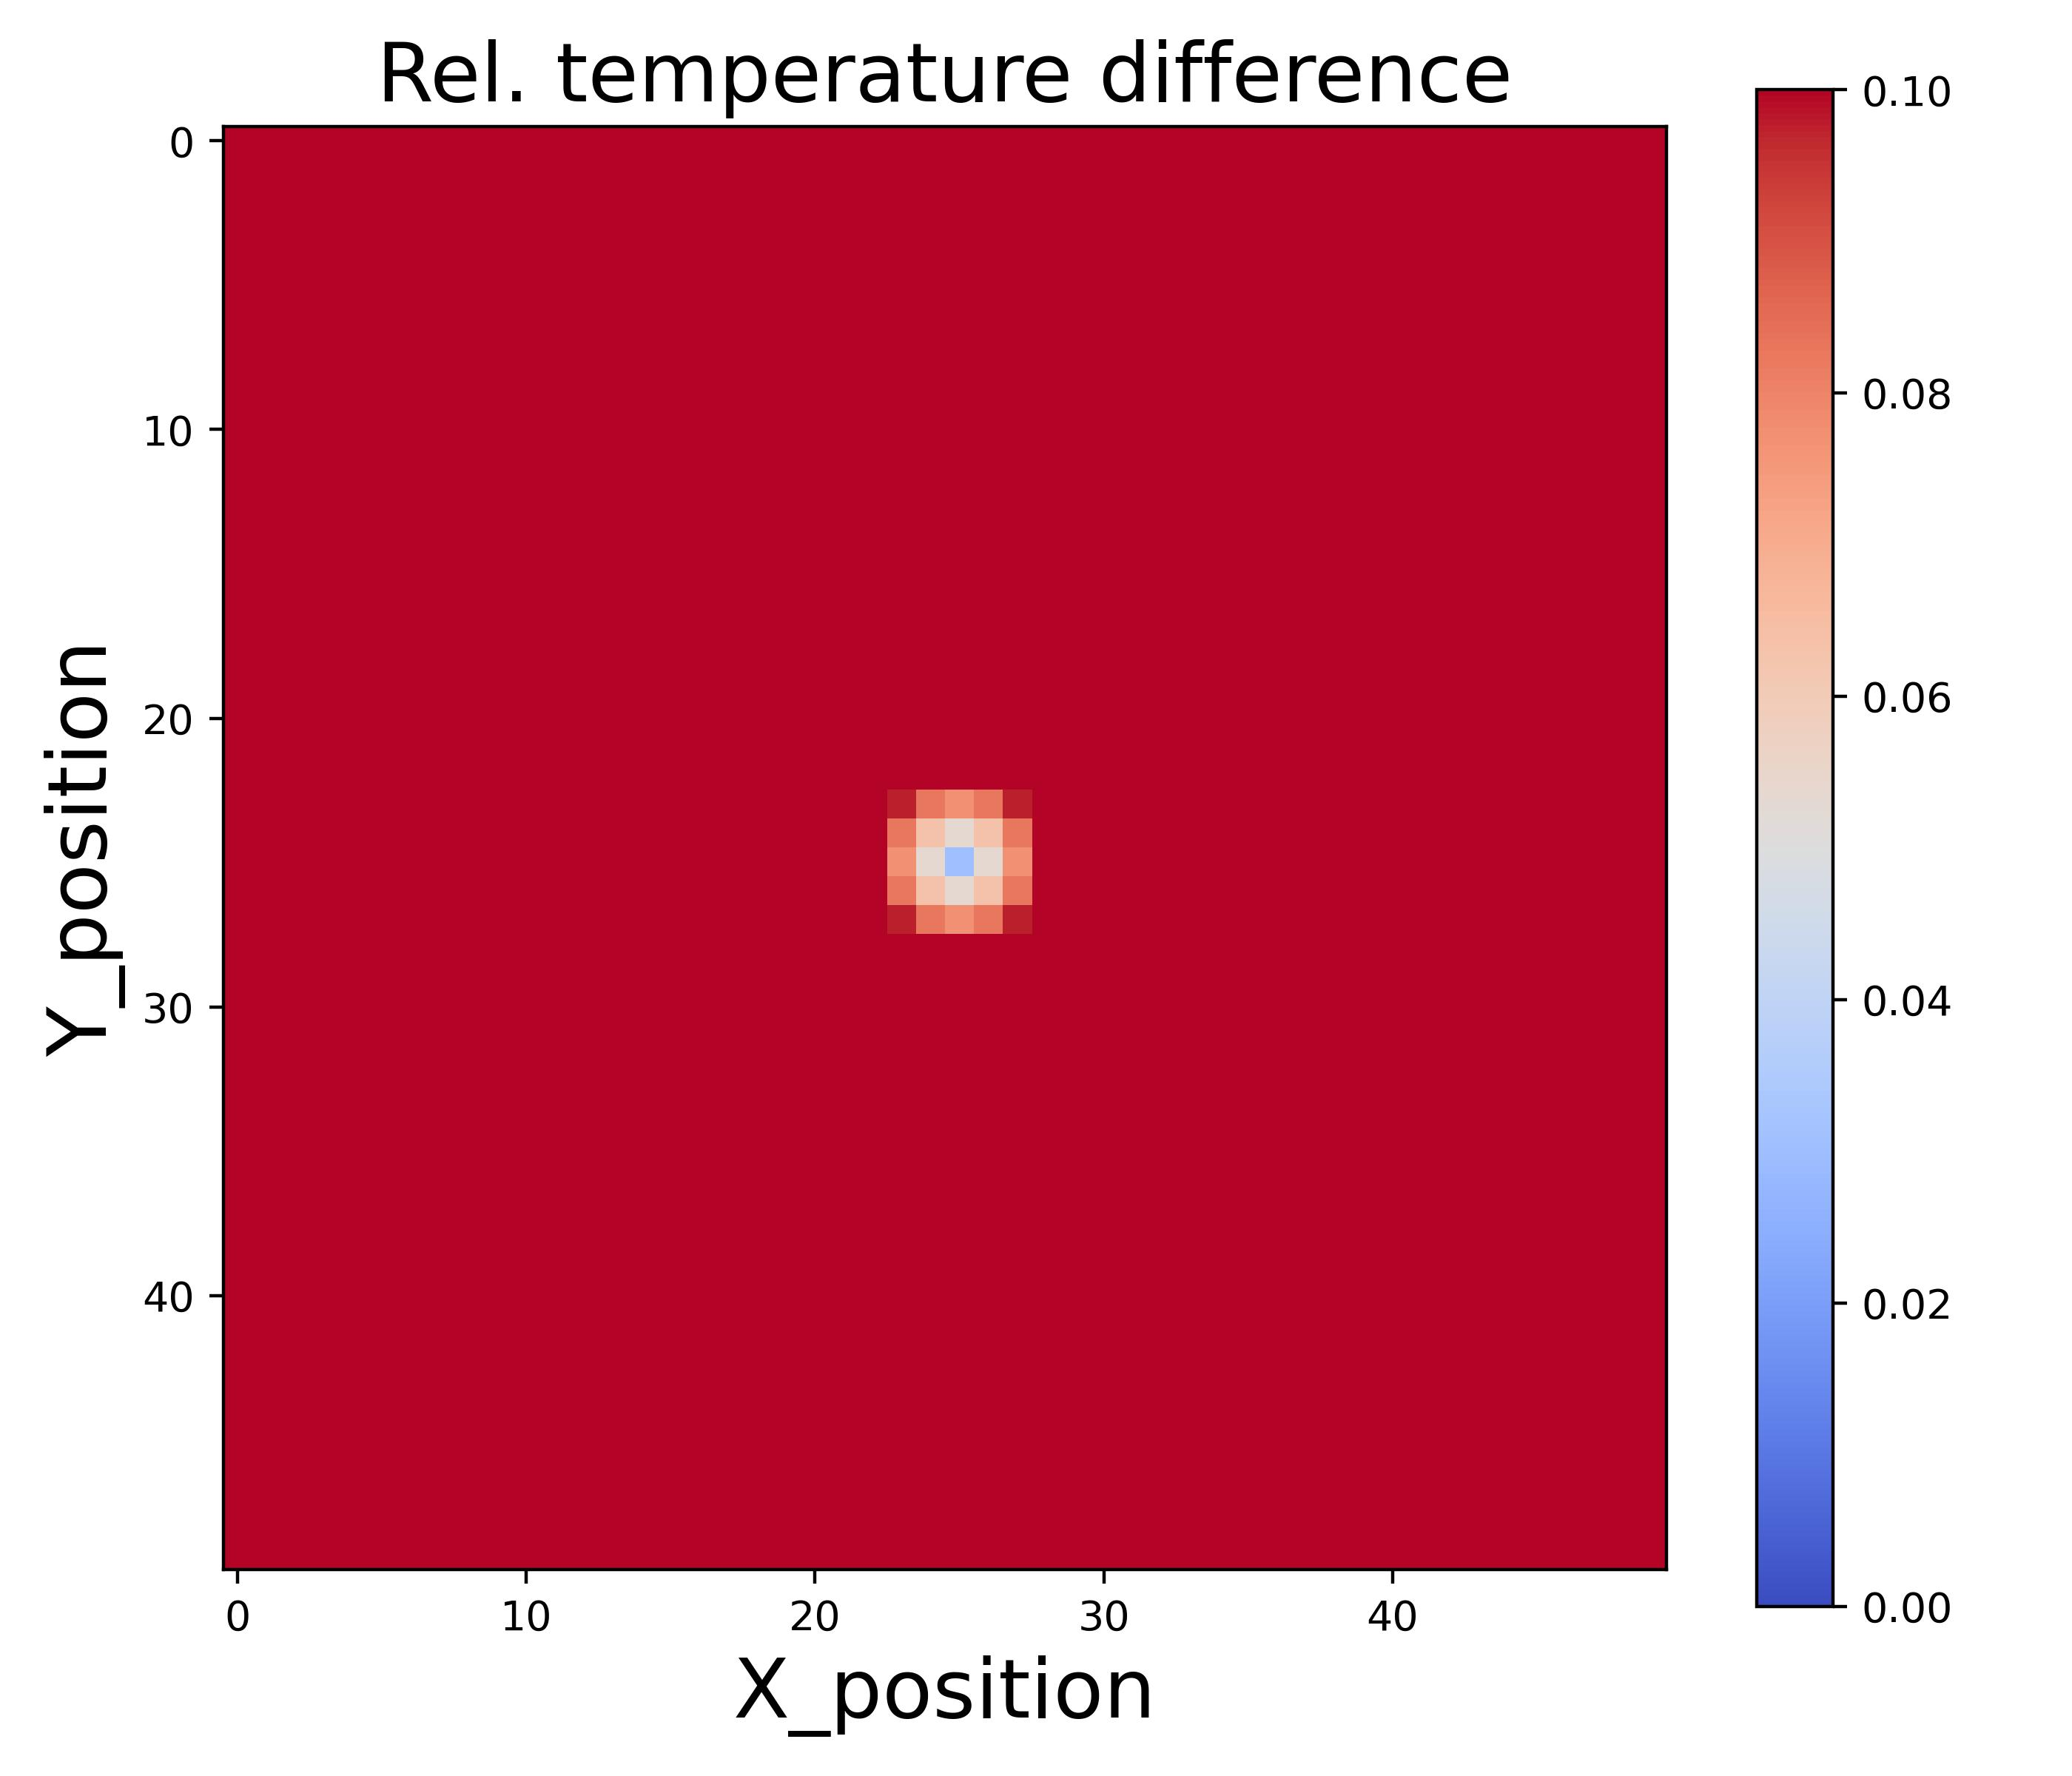
\includegraphics[width=\textwidth]{figures/raw_data/32/lin_square/T_bias.jpg}
            \subcaption{Model 8}
        \end{subfigure}
        \begin{subfigure}{0.27\textwidth}
            \centering
            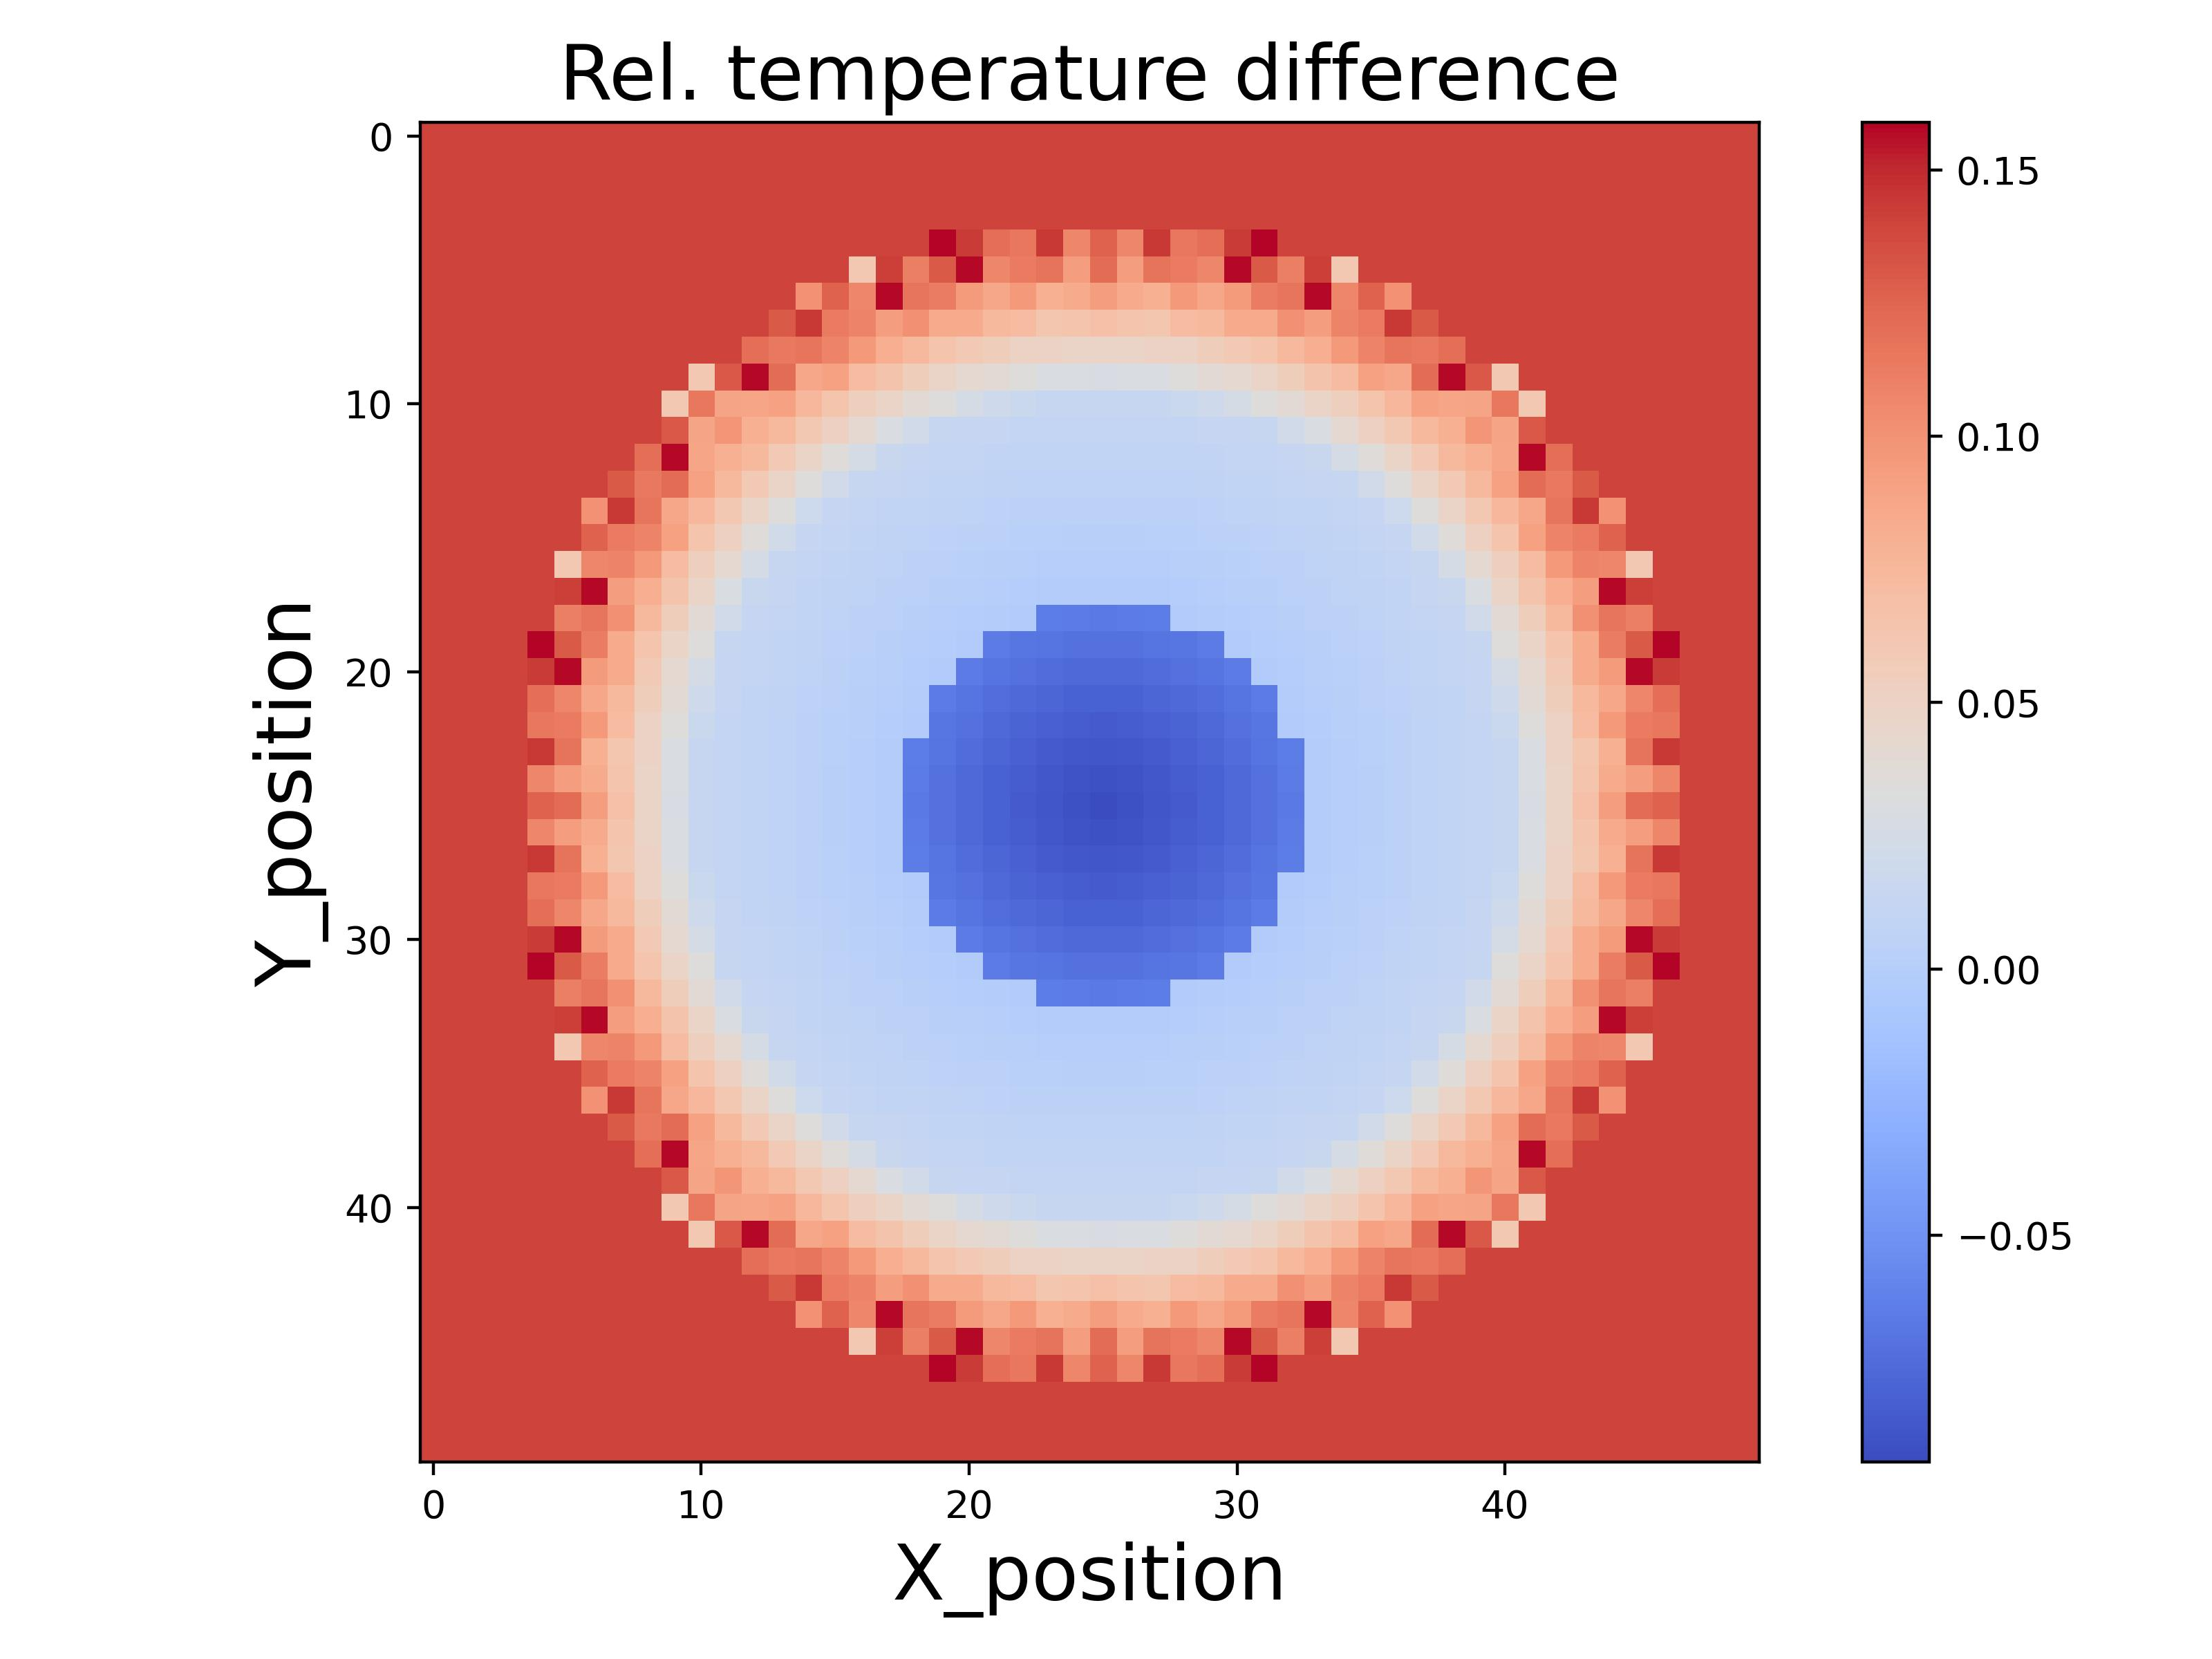
\includegraphics[width=\textwidth]{figures/raw_data/33/lin_square/T_bias.jpg}
            \subcaption{Model 9}
        \end{subfigure}
    \end{minipage}
    \caption{Temperature calculation results of linear square model}  
\end{figure}
\begin{figure}[p]
    \centering
    \begin{minipage}{\textwidth}
        \centering
        \begin{subfigure}{0.325\textwidth}
            \centering
            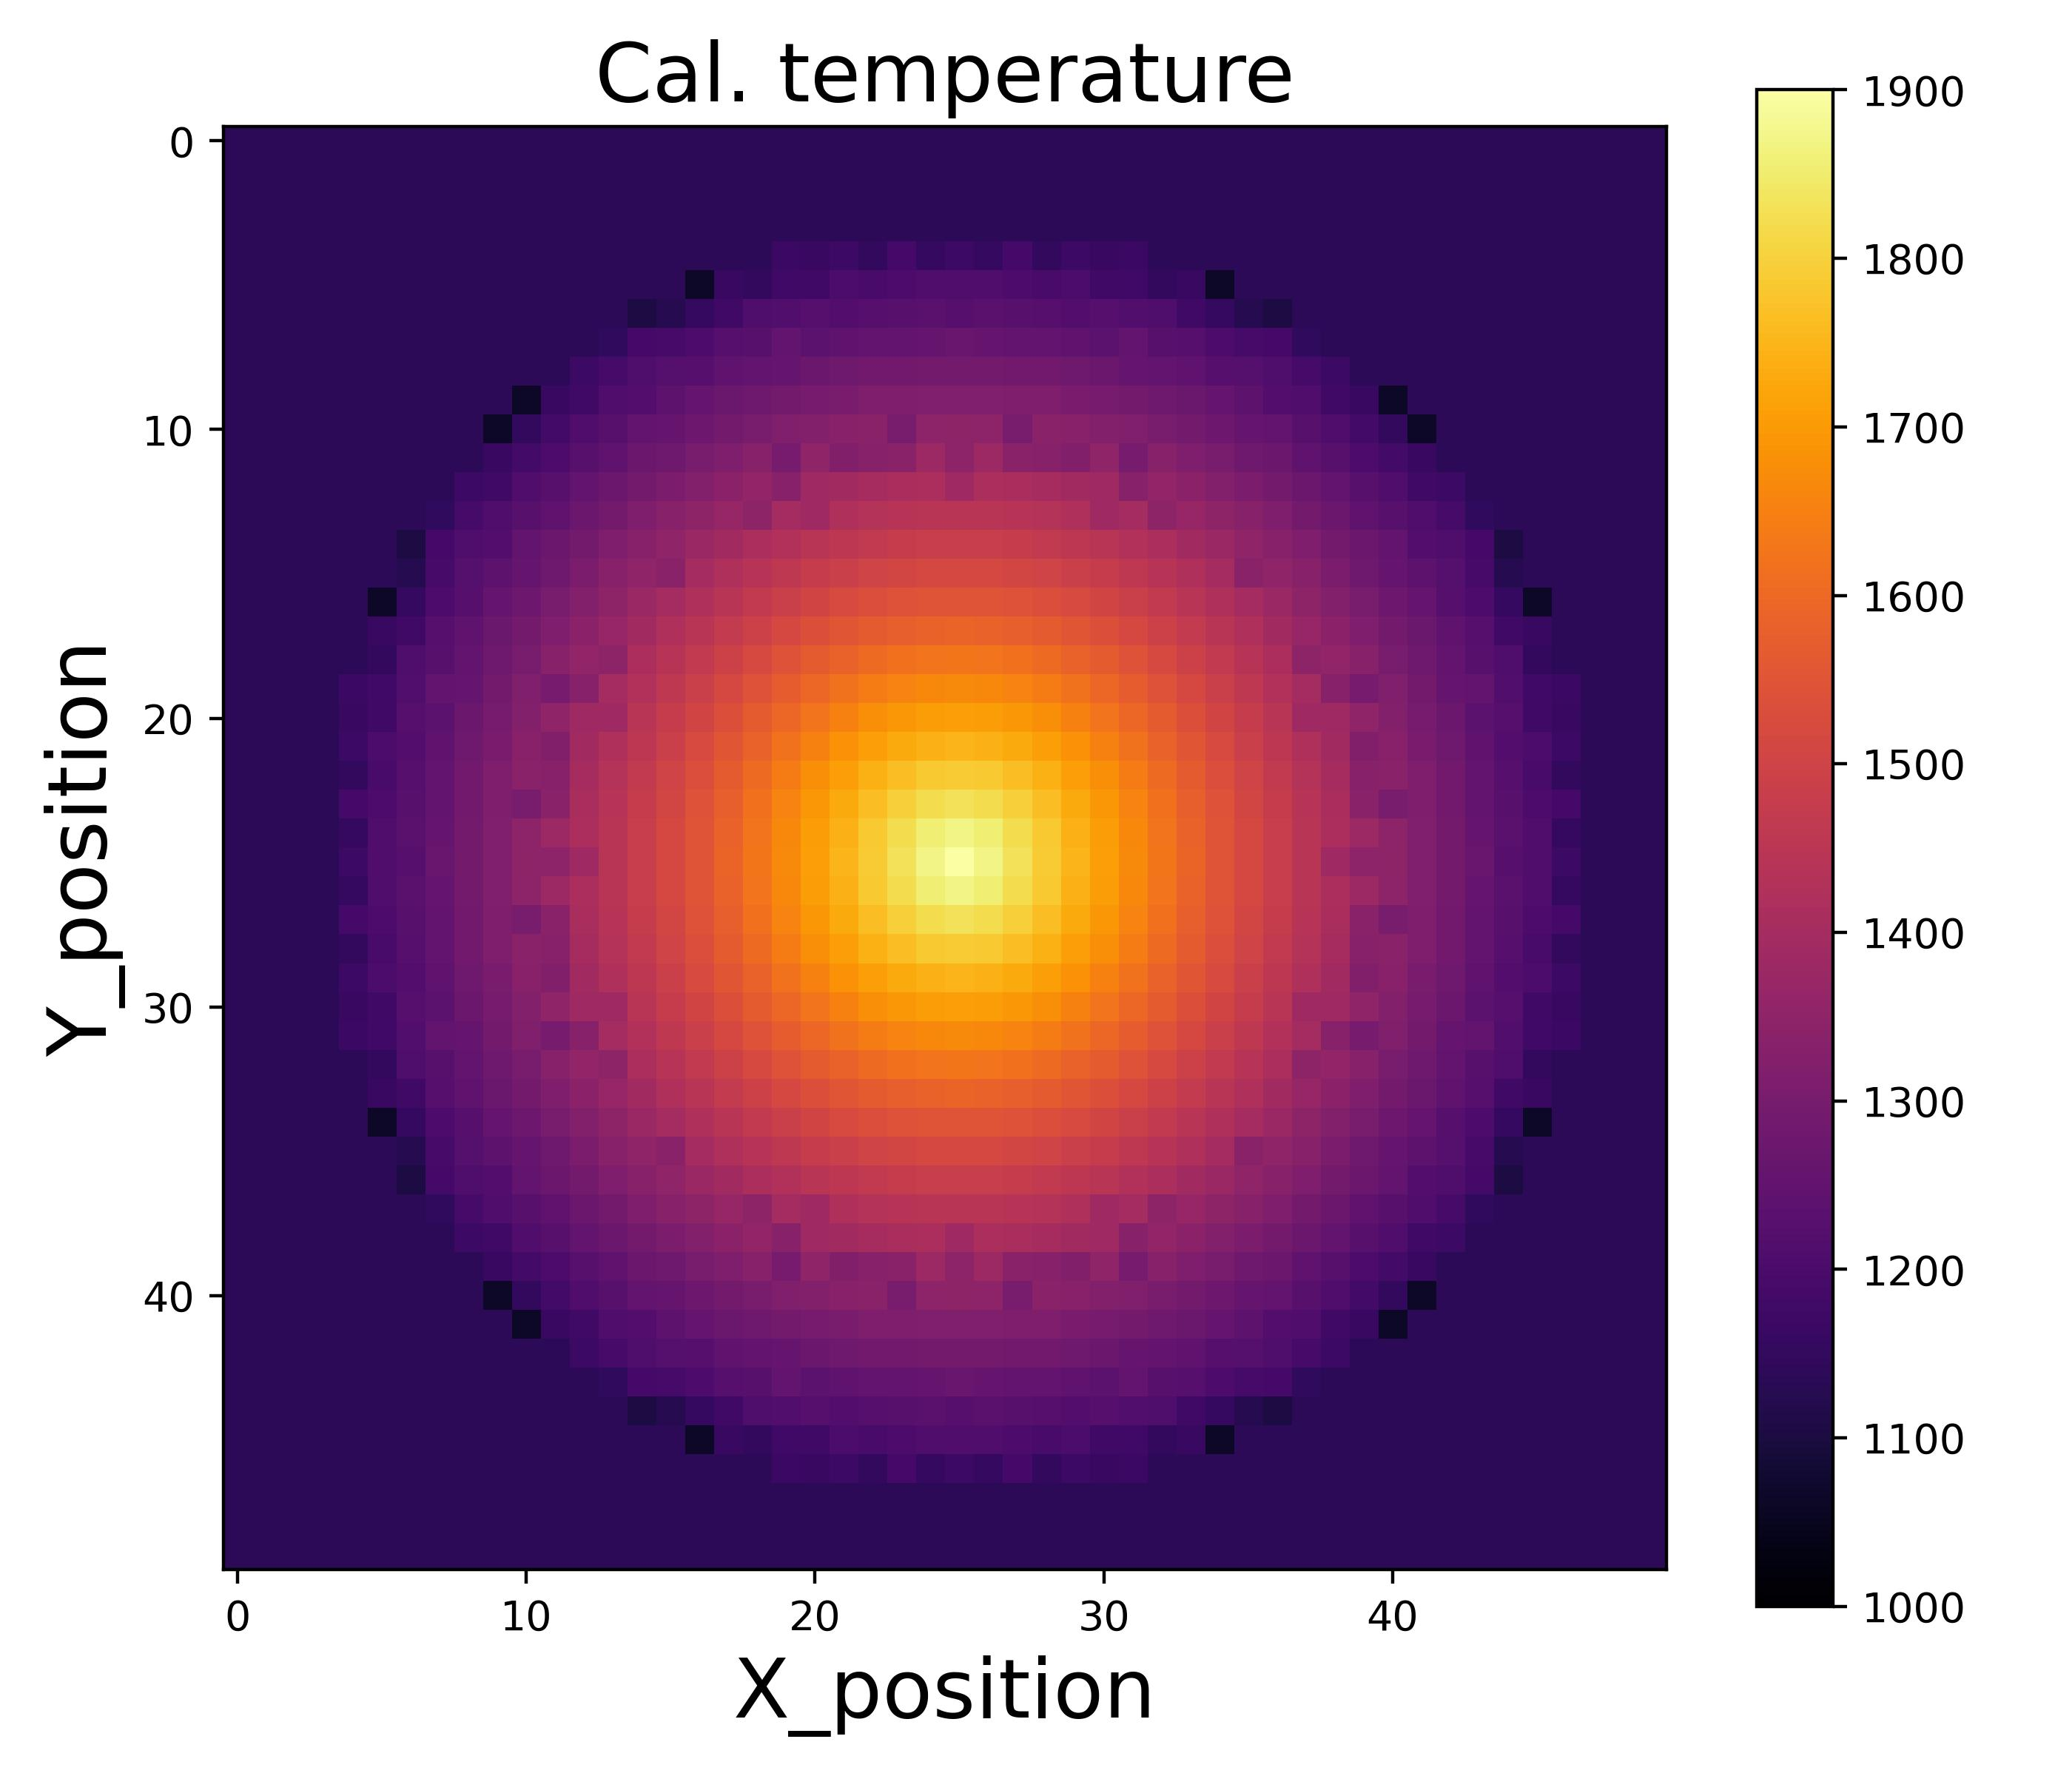
\includegraphics[width=\textwidth]{figures/raw_data/0/lin_square/T_cal.jpg}
            \subcaption{Black body material}
        \end{subfigure}
        \begin{subfigure}{0.325\textwidth}
            \centering
            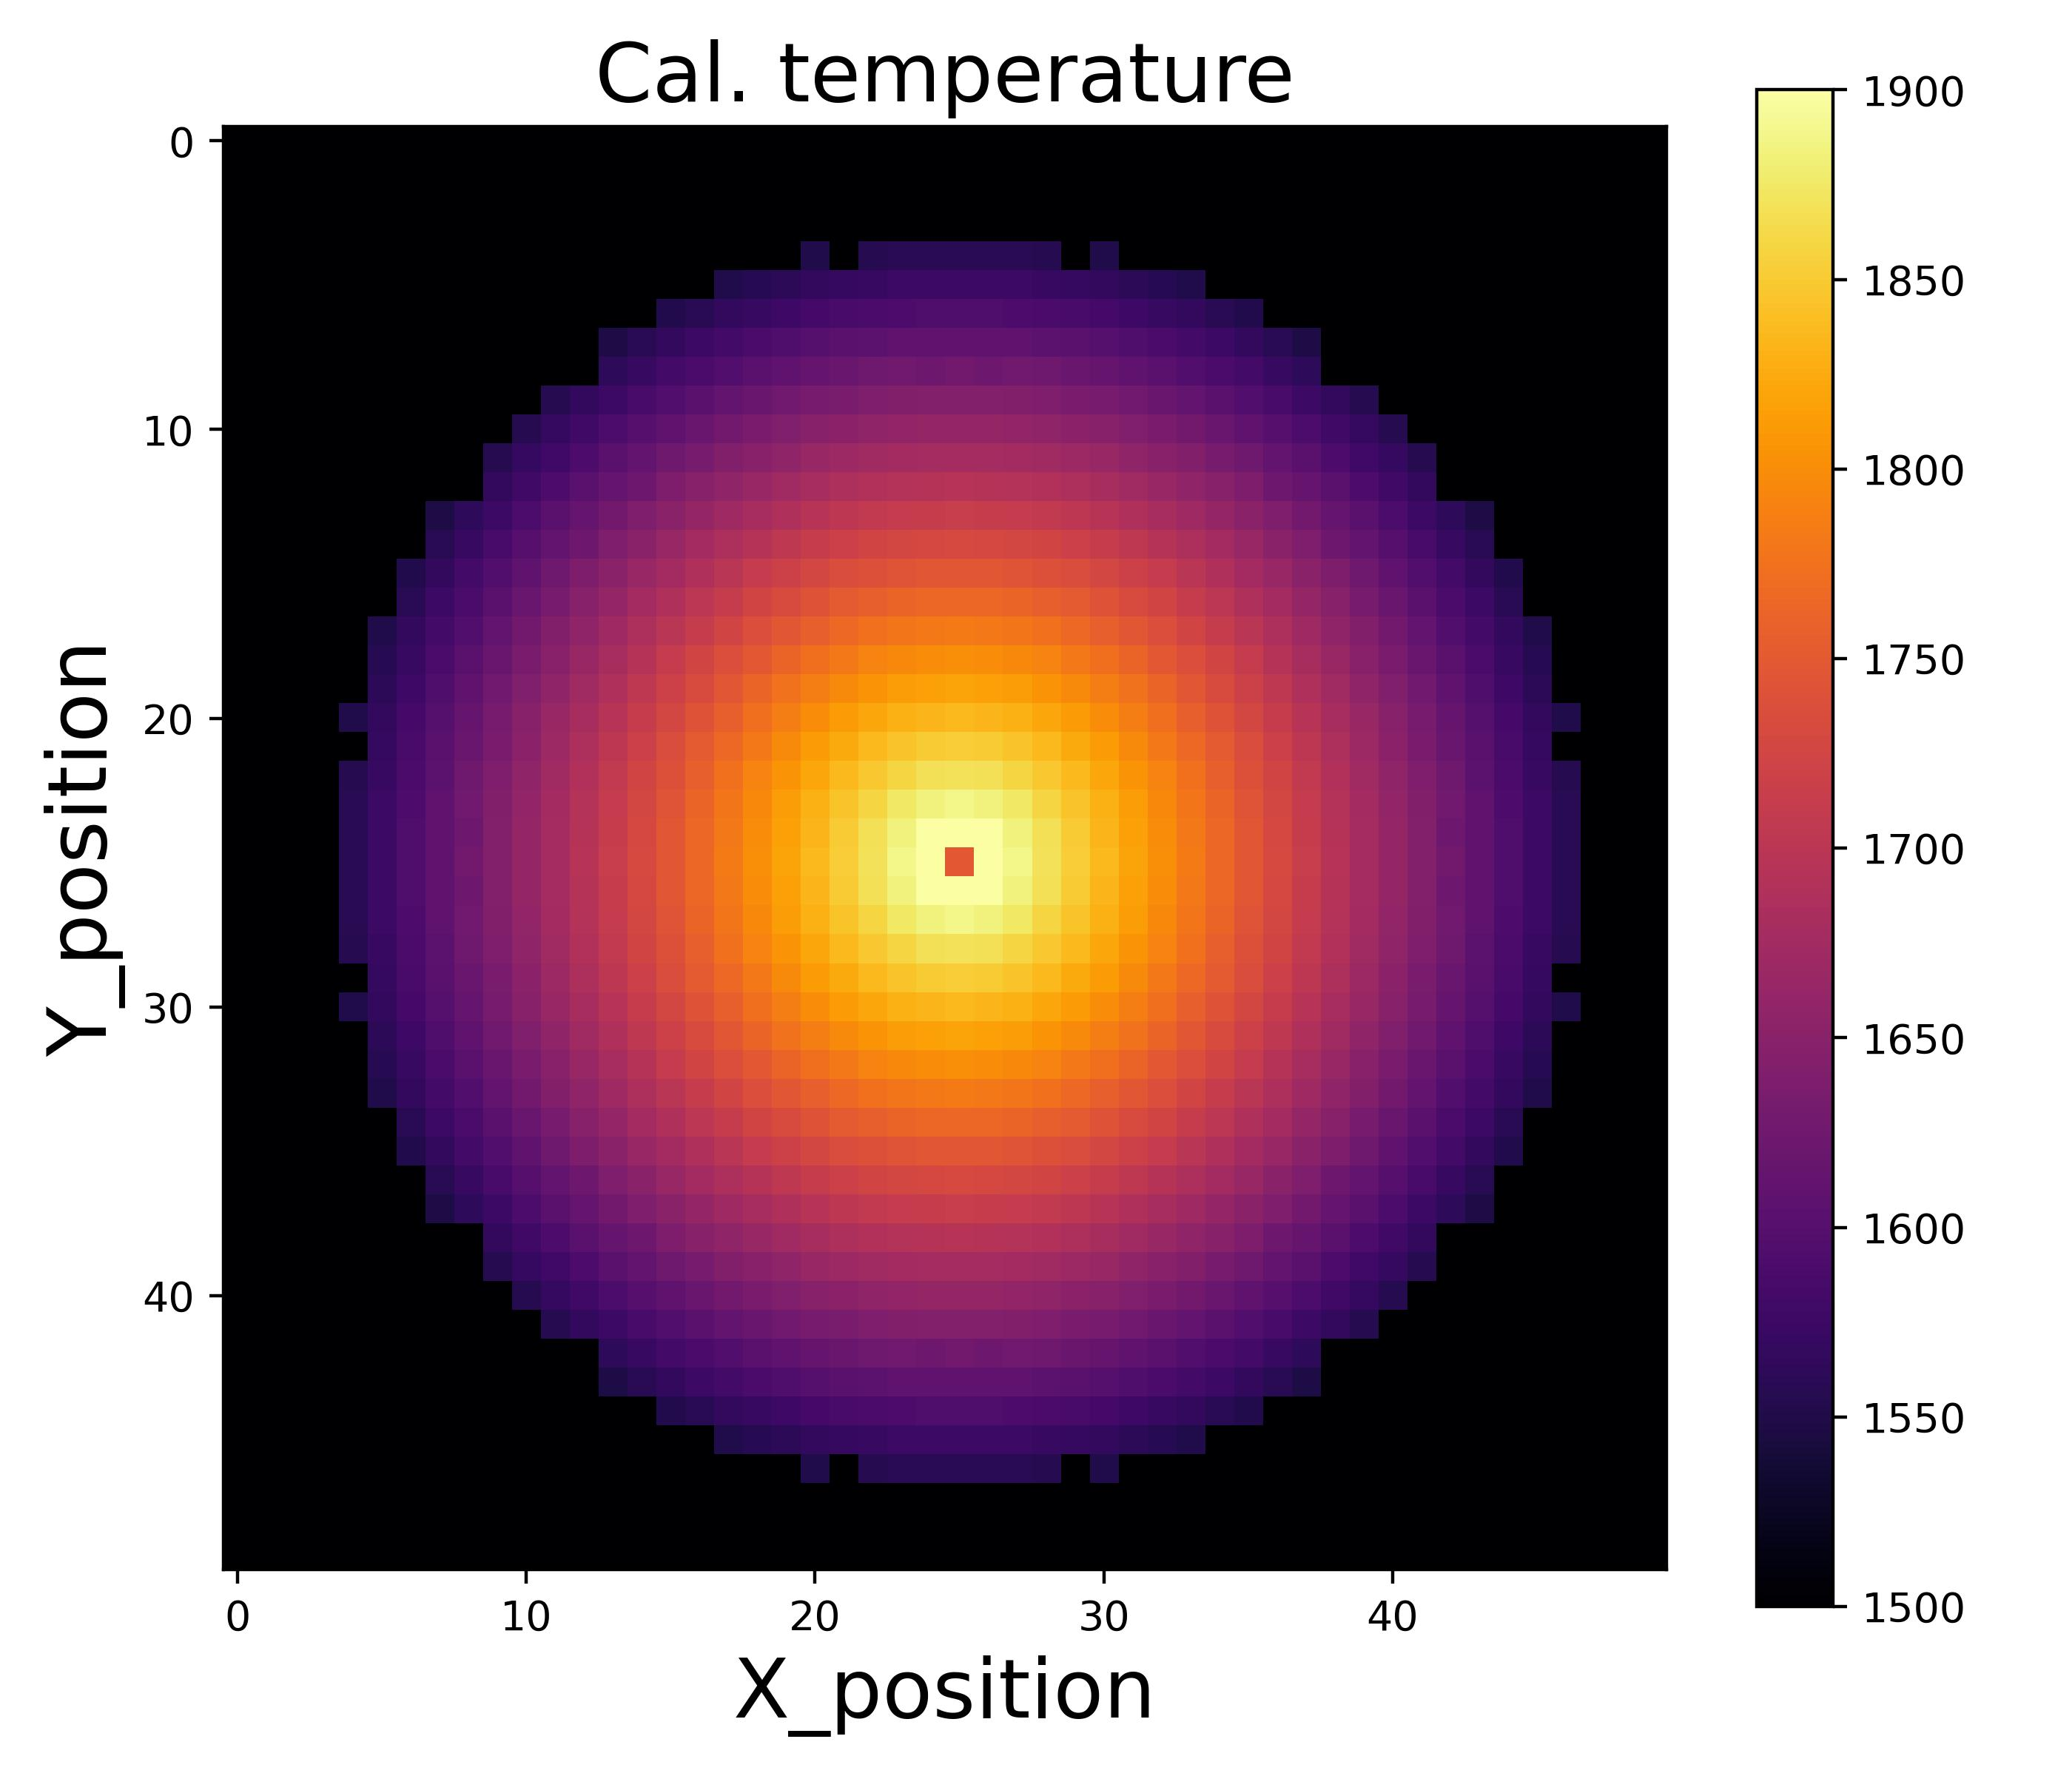
\includegraphics[width=\textwidth]{figures/raw_data/5/lin_square/T_cal.jpg}
            \subcaption{Real iron data}
        \end{subfigure}
        \begin{subfigure}{0.325\textwidth}
            \centering
            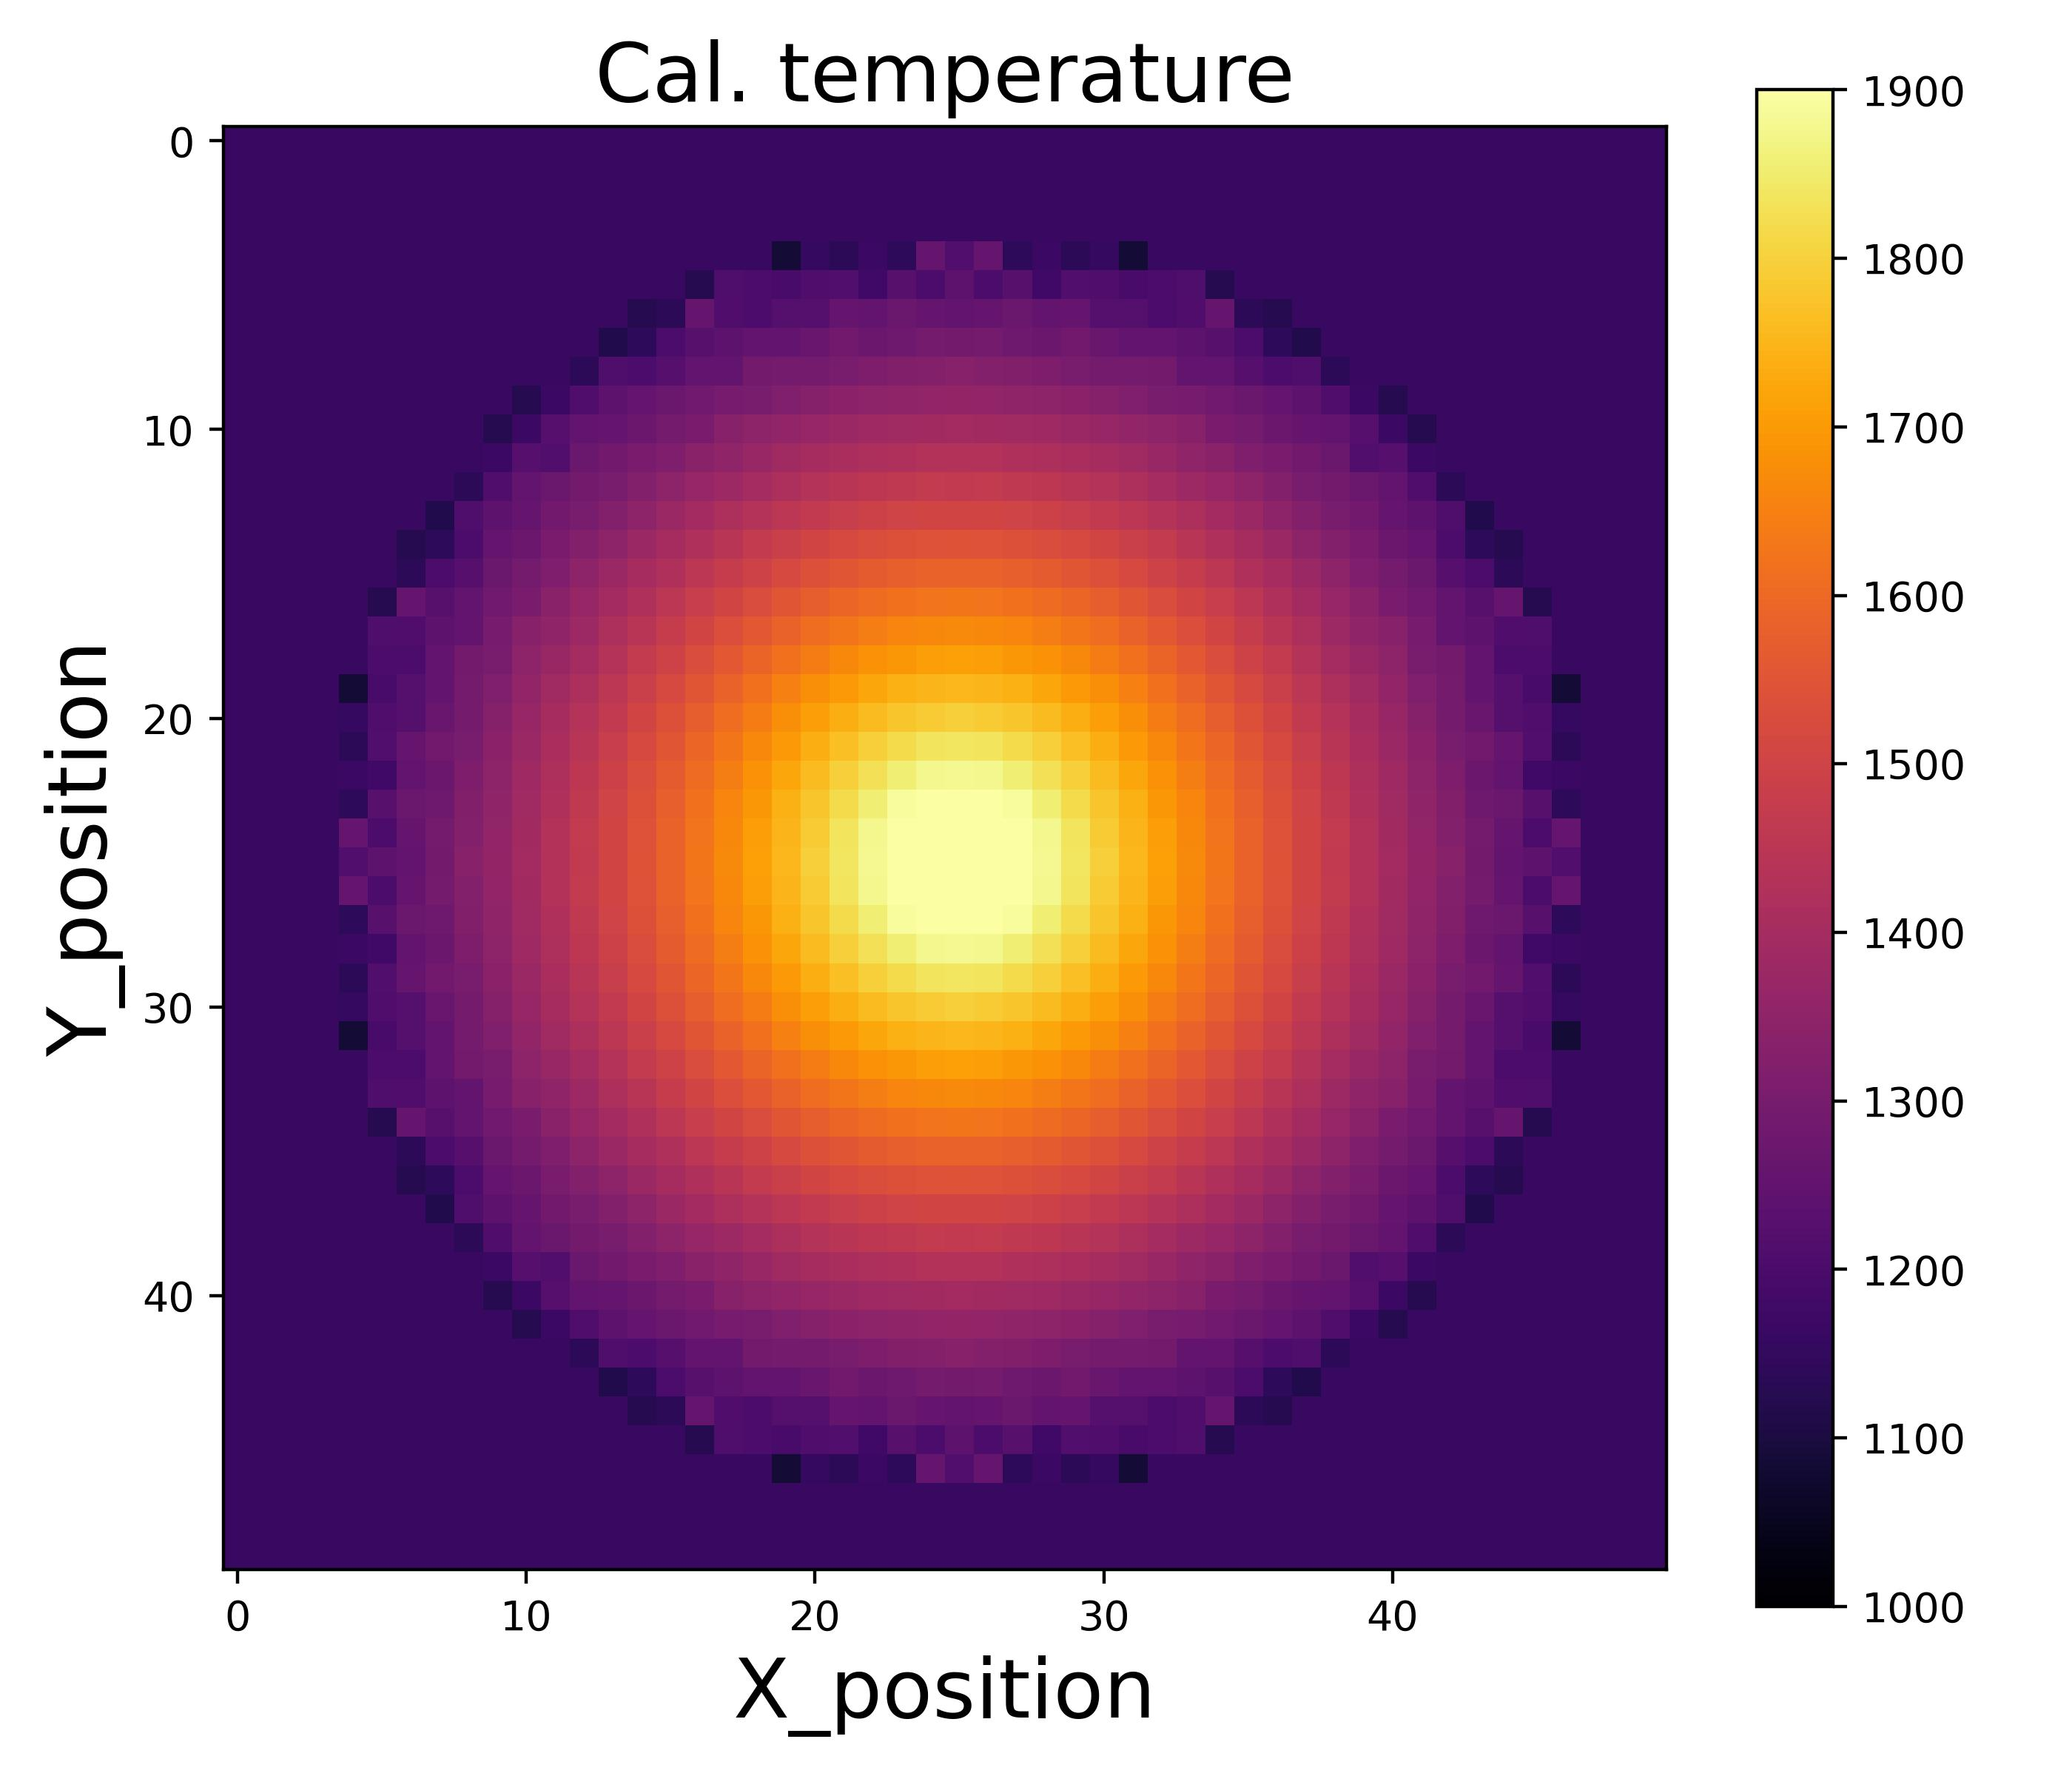
\includegraphics[width=\textwidth]{figures/raw_data/21/lin_square/T_cal.jpg}
            \subcaption{Model 1}
        \end{subfigure}
    \end{minipage}\\
    \begin{minipage}{\textwidth}
        \centering
        \begin{subfigure}{0.325\textwidth}
            \centering
            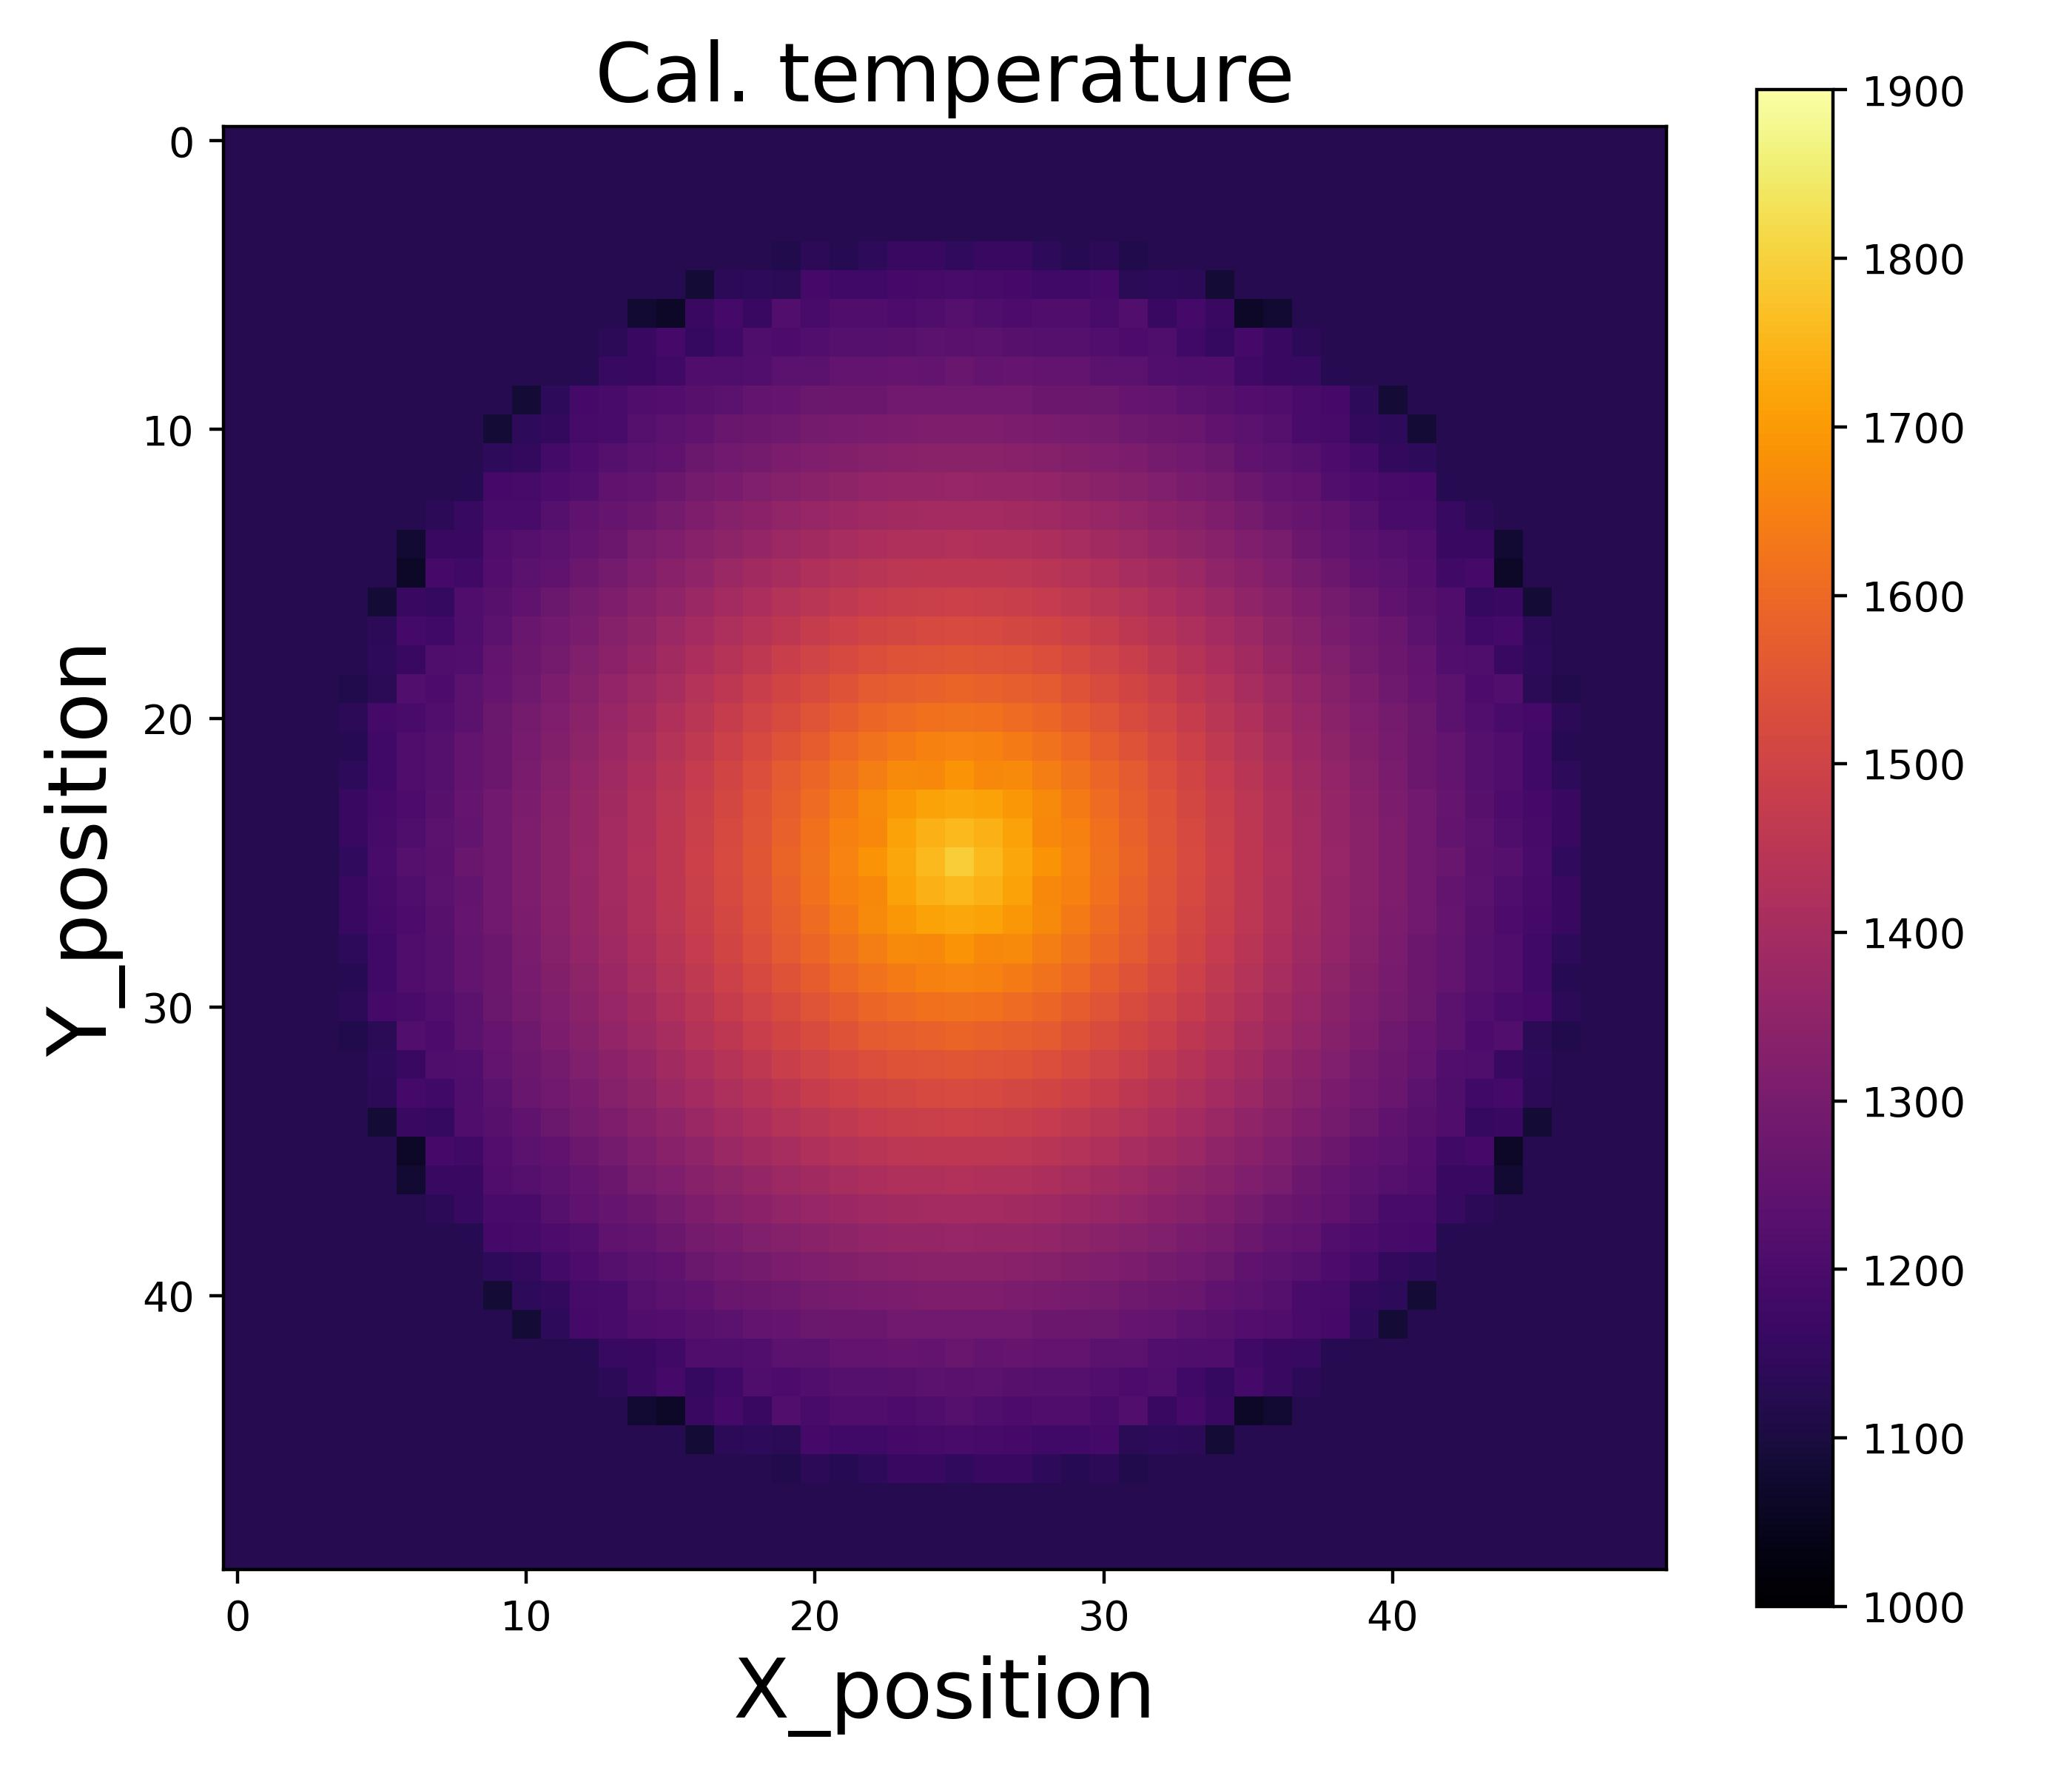
\includegraphics[width=\textwidth]{figures/raw_data/22/lin_square/T_cal.jpg}
            \subcaption{Model 2}
        \end{subfigure}
        \begin{subfigure}{0.325\textwidth}
            \centering
            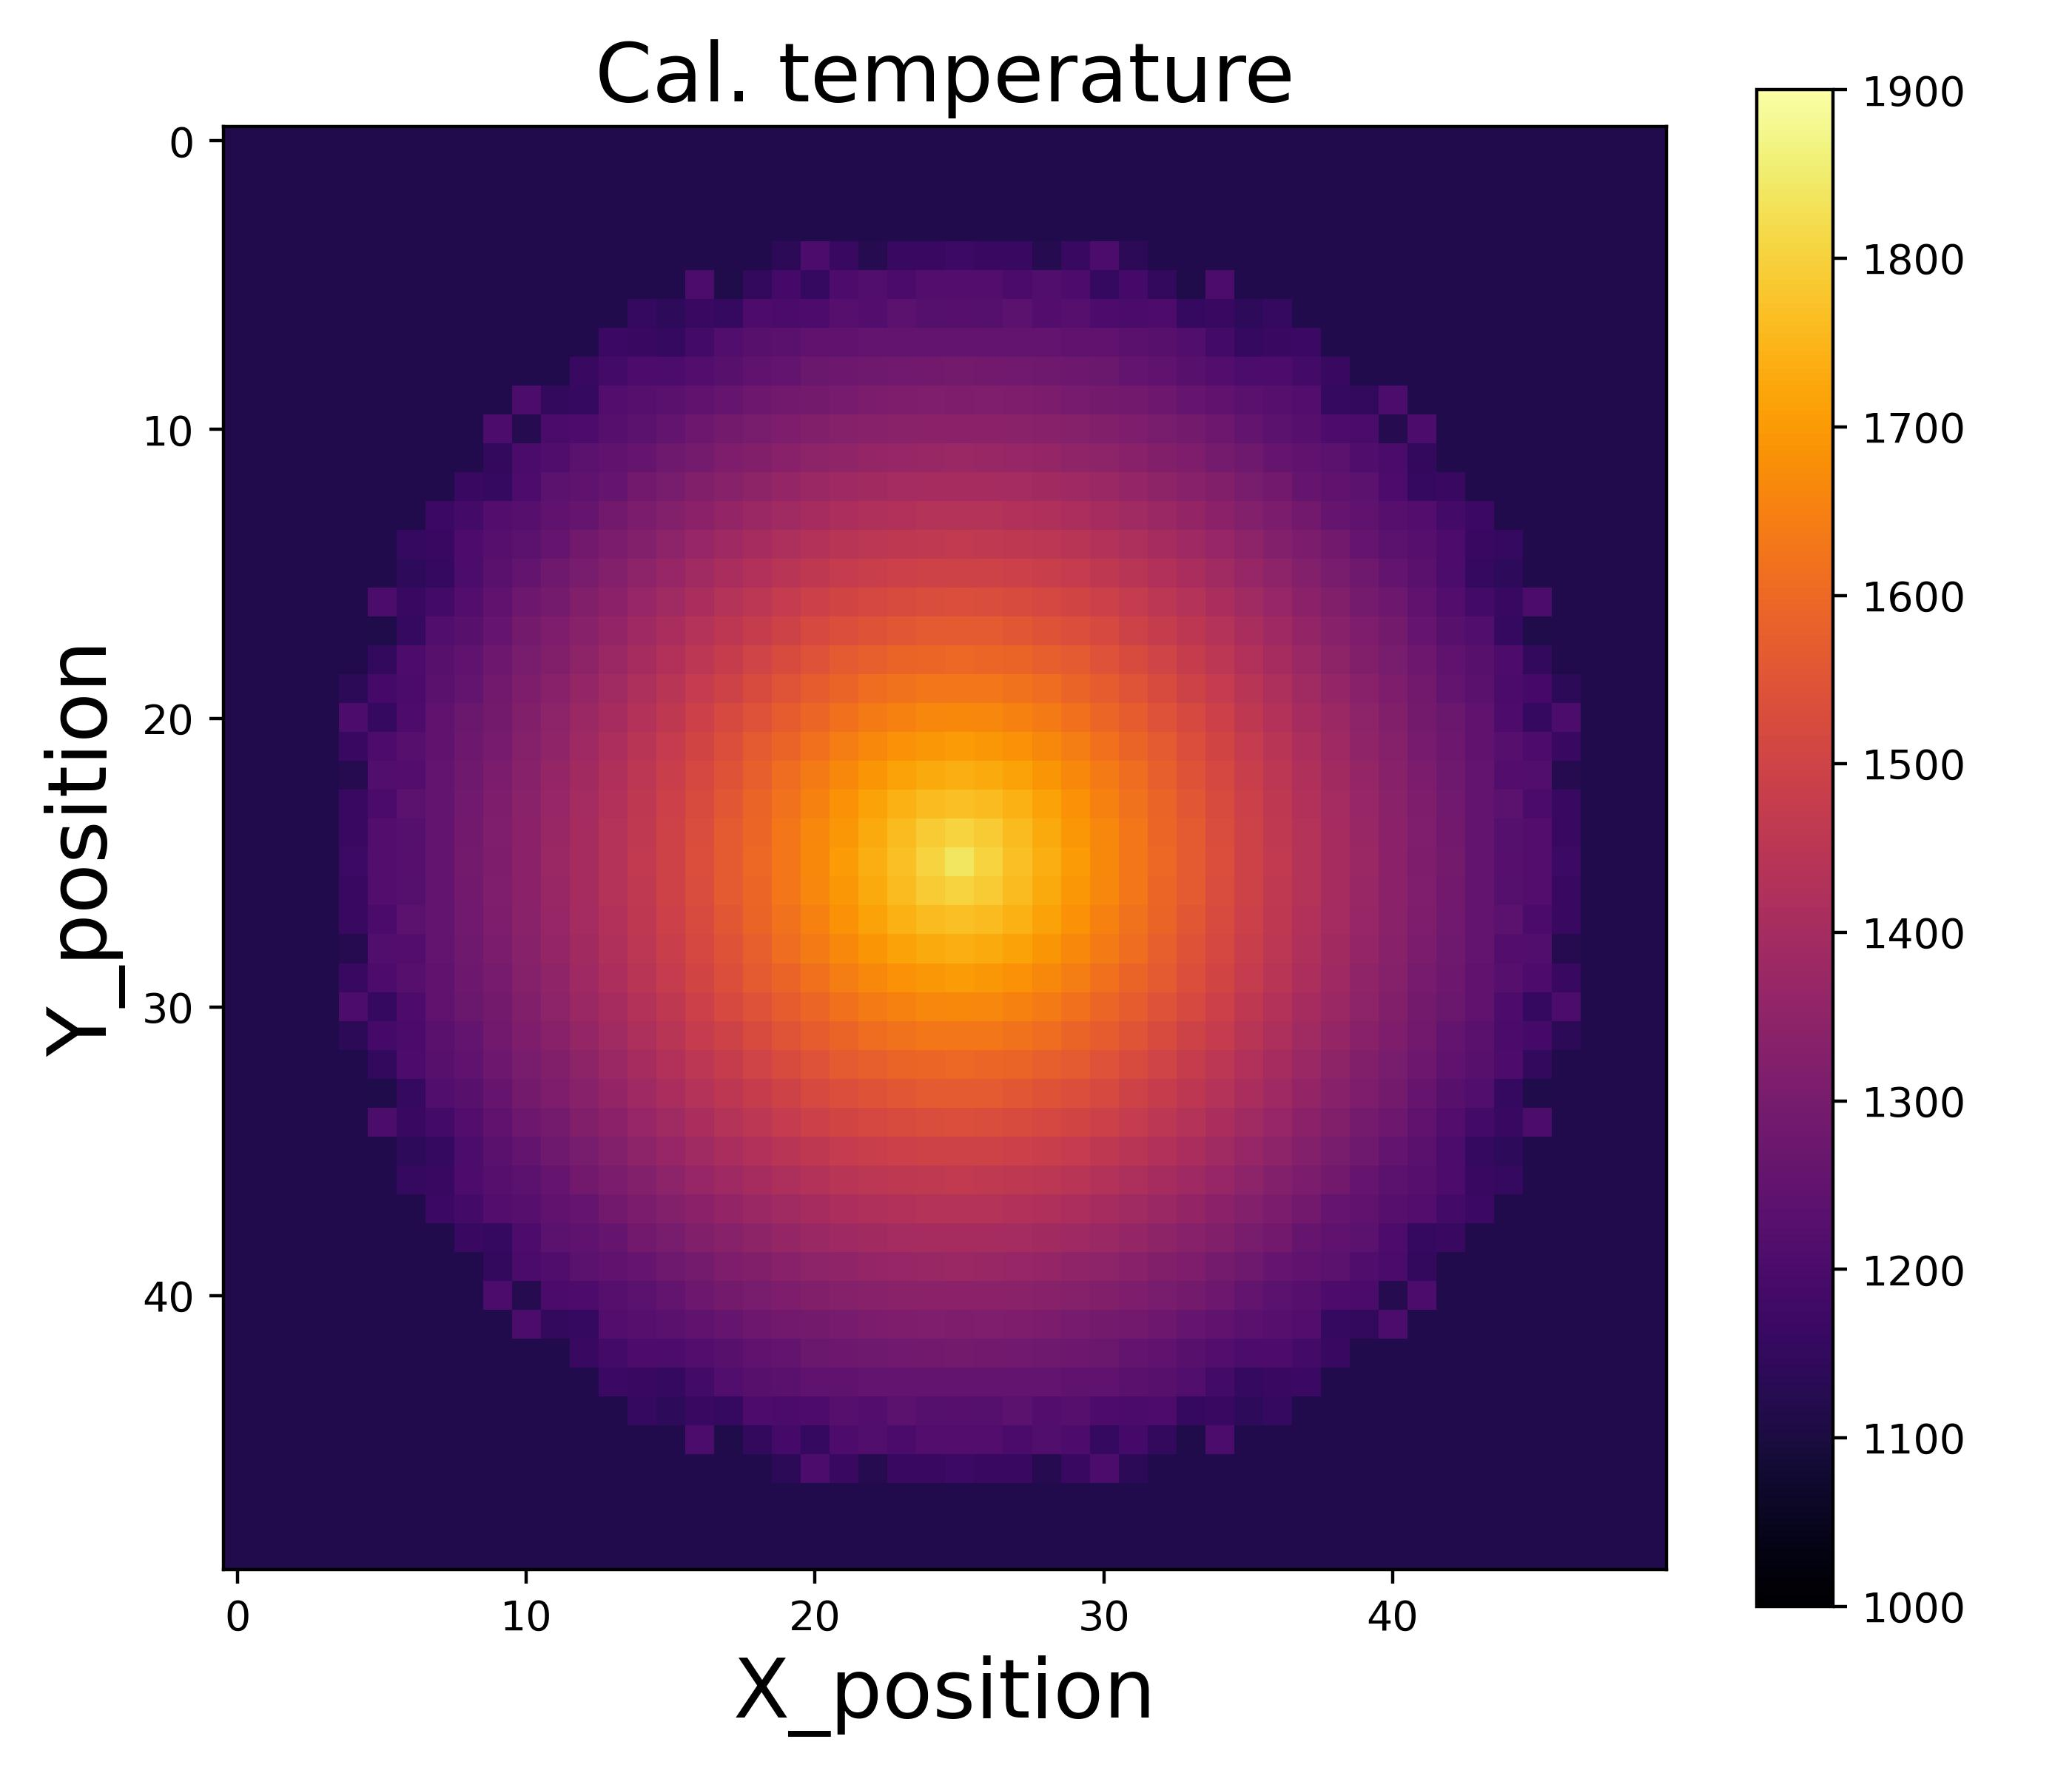
\includegraphics[width=\textwidth]{figures/raw_data/23/lin_square/T_cal.jpg}
            \subcaption{Model 3}
        \end{subfigure}
        \begin{subfigure}{0.325\textwidth}
            \centering
            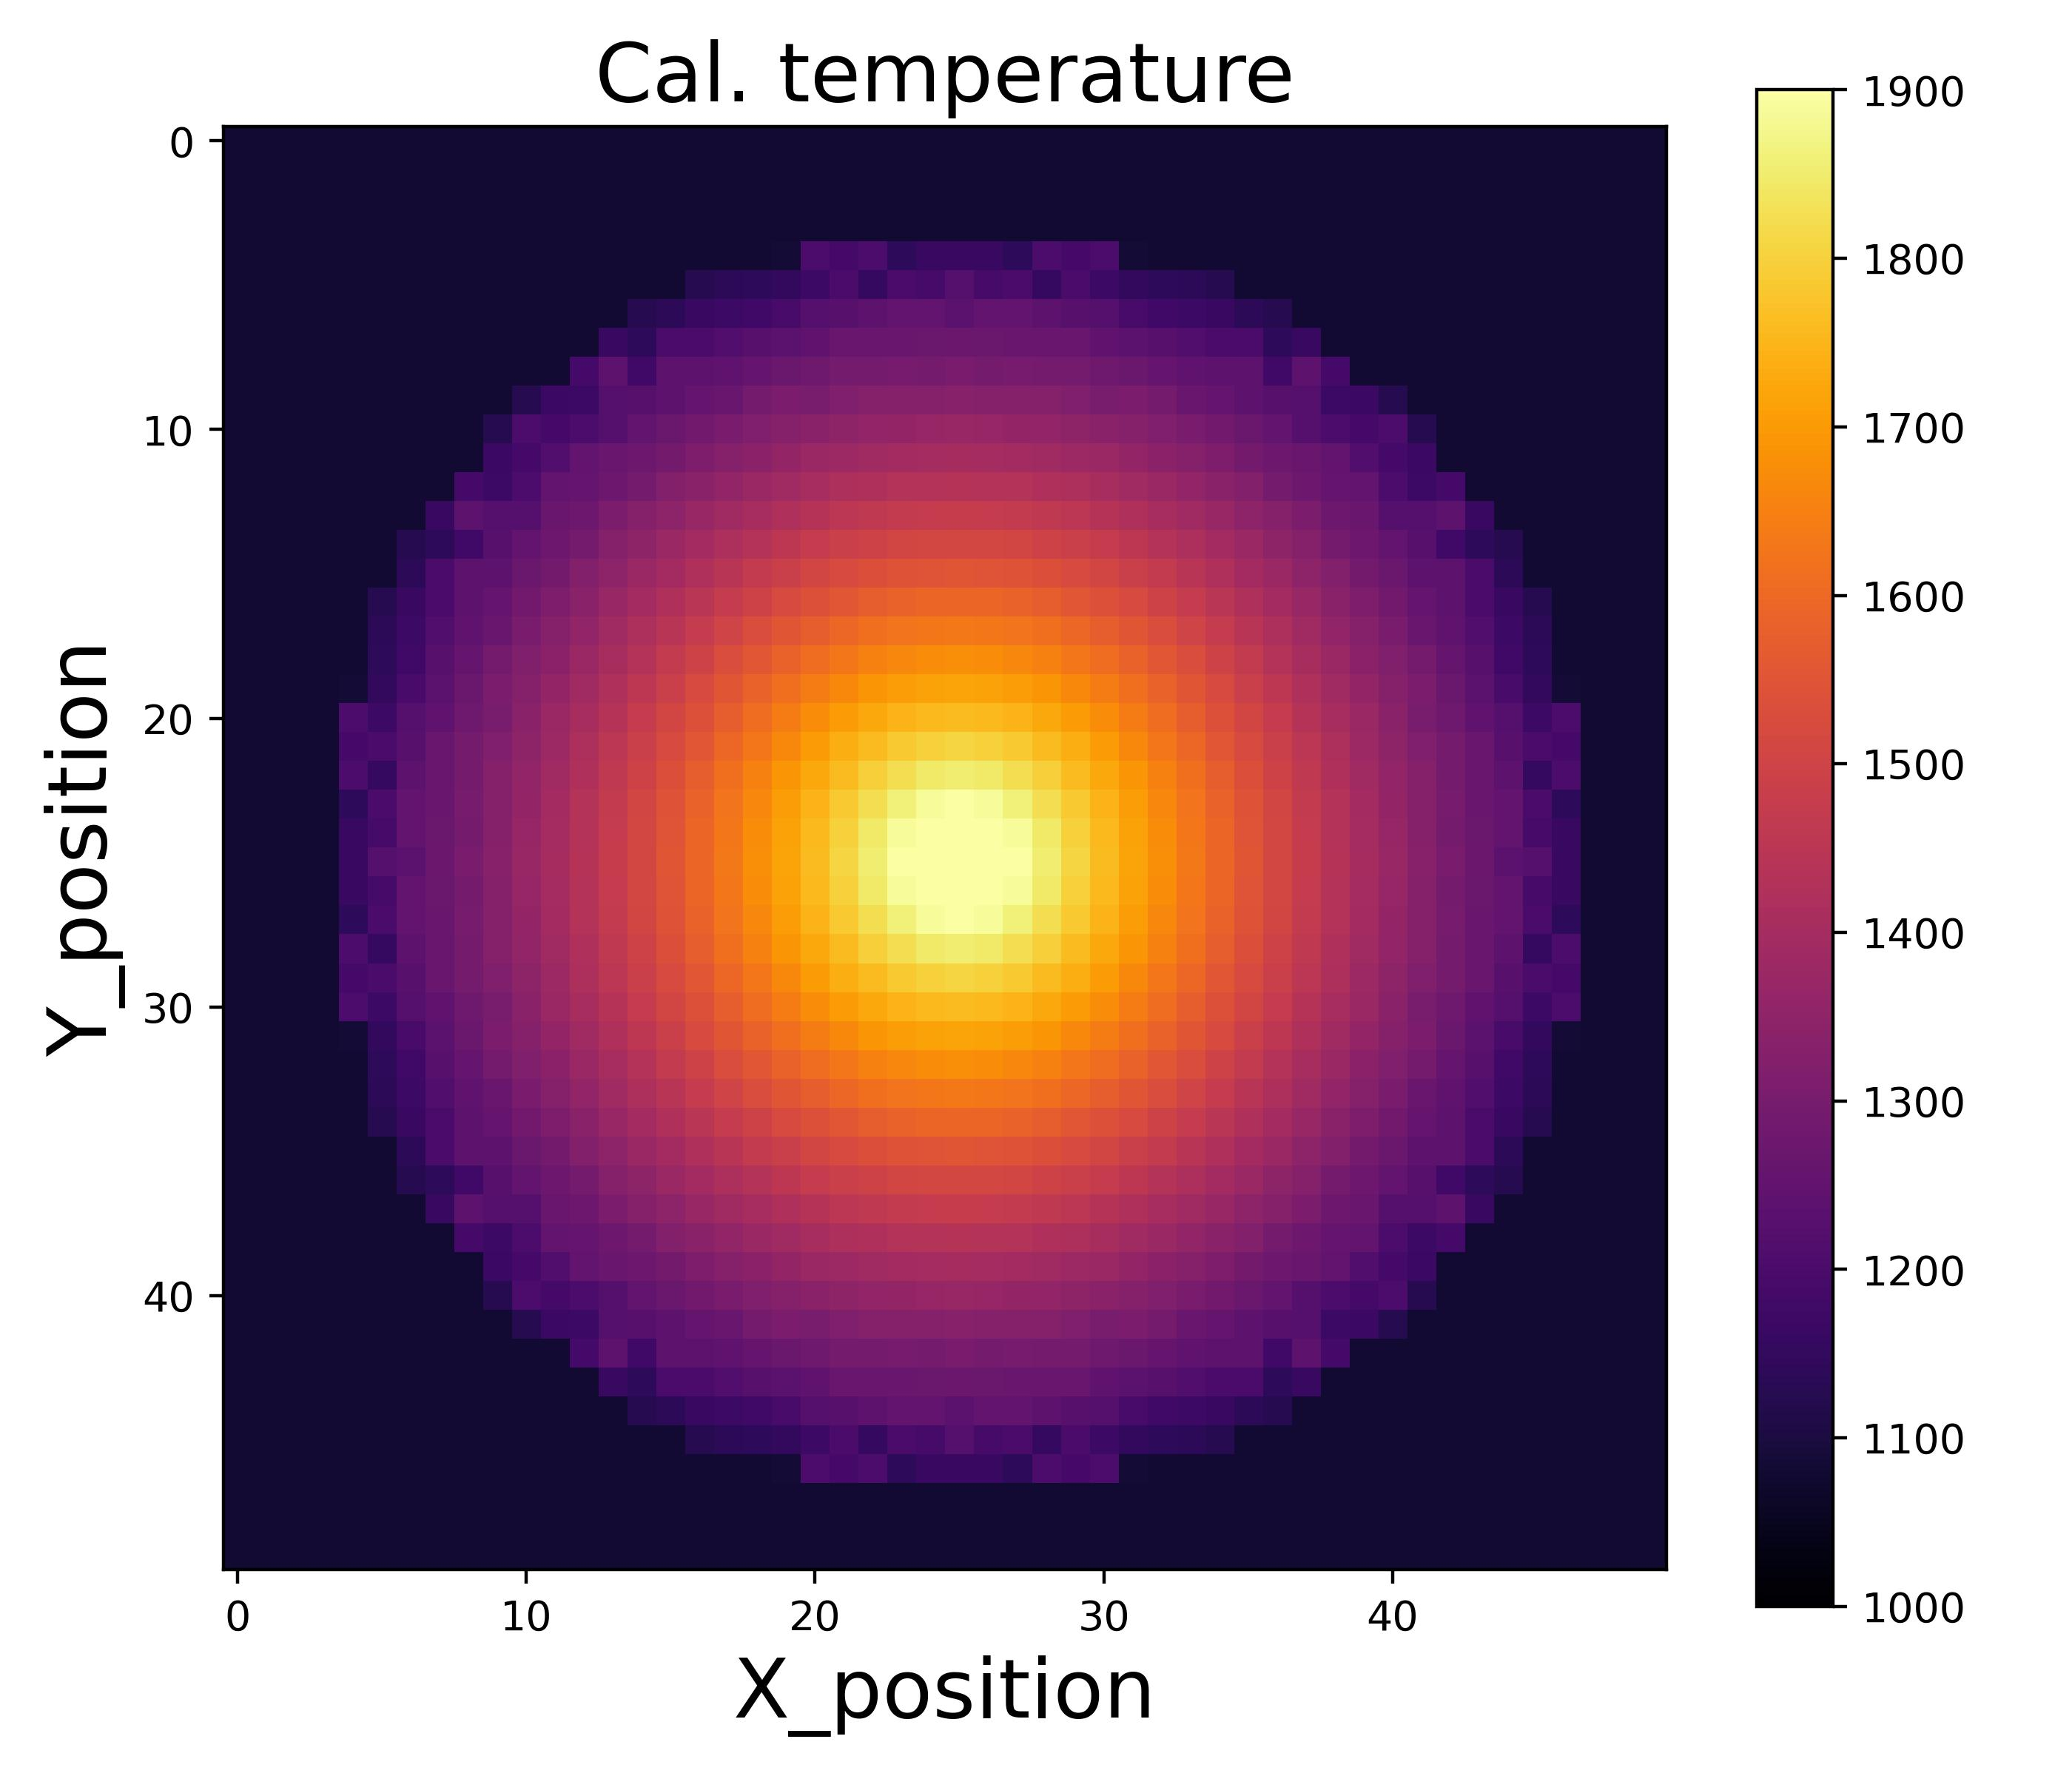
\includegraphics[width=\textwidth]{figures/raw_data/24/lin_square/T_cal.jpg}
            \subcaption{Model 4}
        \end{subfigure}
    \end{minipage}\\
    \begin{minipage}{\textwidth}
        \centering
        \begin{subfigure}{0.325\textwidth}
            \centering
            \includegraphics[width=\textwidth]{figures/raw_data/25/lin_square/T_cal.jpg}
            \subcaption{Model 5}
        \end{subfigure}
        \begin{subfigure}{0.325\textwidth}
            \centering
            \includegraphics[width=\textwidth]{figures/raw_data/26/lin_square/T_cal.jpg}
            \subcaption{Model 6}
        \end{subfigure}
        \begin{subfigure}{0.325\textwidth}
            \centering
            \includegraphics[width=\textwidth]{figures/raw_data/31/lin_square/T_cal.jpg}
            \subcaption{Model 7}
        \end{subfigure}
    \end{minipage}\\
    \begin{minipage}{\textwidth}
        \centering
        \begin{subfigure}{0.325\textwidth}
            \centering
            \includegraphics[width=\textwidth]{figures/raw_data/32/lin_square/T_cal.jpg}
            \subcaption{Model 8}
        \end{subfigure}
        \begin{subfigure}{0.325\textwidth}
            \centering
            \includegraphics[width=\textwidth]{figures/raw_data/33/lin_square/T_cal.jpg}
            \subcaption{Model 9}
        \end{subfigure}
    \end{minipage}
    \caption{Temperature calculation results of linear square model}  
\end{figure}
\begin{figure}[p]
    \centering
    \begin{minipage}{\textwidth}
        \centering
        \begin{subfigure}{0.325\textwidth}
            \centering
            \includegraphics[width=\textwidth]{figures/raw_data/0/lin_square/emi_cal.jpg}
            \subcaption{Black body material}
        \end{subfigure}
        \begin{subfigure}{0.325\textwidth}
            \centering
            \includegraphics[width=\textwidth]{figures/raw_data/5/lin_square/emi_cal.jpg}
            \subcaption{Real iron data}
        \end{subfigure}
        \begin{subfigure}{0.325\textwidth}
            \centering
            \includegraphics[width=\textwidth]{figures/raw_data/21/lin_square/emi_cal.jpg}
            \subcaption{Model 1}
        \end{subfigure}
    \end{minipage}\\
    \begin{minipage}{\textwidth}
        \centering
        \begin{subfigure}{0.325\textwidth}
            \centering
            \includegraphics[width=\textwidth]{figures/raw_data/22/lin_square/emi_cal.jpg}
            \subcaption{Model 2}
        \end{subfigure}
        \begin{subfigure}{0.325\textwidth}
            \centering
            \includegraphics[width=\textwidth]{figures/raw_data/23/lin_square/emi_cal.jpg}
            \subcaption{Model 3}
        \end{subfigure}
        \begin{subfigure}{0.325\textwidth}
            \centering
            \includegraphics[width=\textwidth]{figures/raw_data/24/lin_square/emi_cal.jpg}
            \subcaption{Model 4}
        \end{subfigure}
    \end{minipage}\\
    \begin{minipage}{\textwidth}
        \centering
        \begin{subfigure}{0.325\textwidth}
            \centering
            \includegraphics[width=\textwidth]{figures/raw_data/25/lin_square/emi_cal.jpg}
            \subcaption{Model 5}
        \end{subfigure}
        \begin{subfigure}{0.325\textwidth}
            \centering
            \includegraphics[width=\textwidth]{figures/raw_data/26/lin_square/emi_cal.jpg}
            \subcaption{Model 6}
        \end{subfigure}
        \begin{subfigure}{0.325\textwidth}
            \centering
            \includegraphics[width=\textwidth]{figures/raw_data/31/lin_square/emi_cal.jpg}
            \subcaption{Model 7}
        \end{subfigure}
    \end{minipage}\\
    \begin{minipage}{\textwidth}
        \centering
        \begin{subfigure}{0.325\textwidth}
            \centering
            \includegraphics[width=\textwidth]{figures/raw_data/32/lin_square/emi_cal.jpg}
            \subcaption{Model 8}
        \end{subfigure}
        \begin{subfigure}{0.325\textwidth}
            \centering
            \includegraphics[width=\textwidth]{figures/raw_data/33/lin_square/emi_cal.jpg}
            \subcaption{Model 9}
        \end{subfigure}
    \end{minipage}
    \caption{Emissivity calculation results of linear square model}  
\end{figure}


\newpage
\subsection{Quadratic model}
\begin{figure}[h]
    \centering
    \begin{minipage}{\textwidth}
        \centering
        \begin{subfigure}{0.27\textwidth}
            \centering
            \includegraphics[width=\textwidth]{figures/raw_data/0/quad/T_bias.jpg}
            \subcaption{Black body material}
        \end{subfigure}
        \begin{subfigure}{0.27\textwidth}
            \centering
            \includegraphics[width=\textwidth]{figures/raw_data/5/quad/T_bias.jpg}
            \subcaption{Real iron data}
        \end{subfigure}
        \begin{subfigure}{0.27\textwidth}
            \centering
            \includegraphics[width=\textwidth]{figures/raw_data/21/quad/T_bias.jpg}
            \subcaption{Model 1}
        \end{subfigure}
    \end{minipage}\\
    \begin{minipage}{\textwidth}
        \centering
        \begin{subfigure}{0.27\textwidth}
            \centering
            \includegraphics[width=\textwidth]{figures/raw_data/22/quad/T_bias.jpg}
            \subcaption{Model 2}
        \end{subfigure}
        \begin{subfigure}{0.27\textwidth}
            \centering
            \includegraphics[width=\textwidth]{figures/raw_data/23/quad/T_bias.jpg}
            \subcaption{Model 3}
        \end{subfigure}
        \begin{subfigure}{0.27\textwidth}
            \centering
            \includegraphics[width=\textwidth]{figures/raw_data/24/quad/T_bias.jpg}
            \subcaption{Model 4}
        \end{subfigure}
    \end{minipage}\\
    \begin{minipage}{\textwidth}
        \centering
        \begin{subfigure}{0.27\textwidth}
            \centering
            \includegraphics[width=\textwidth]{figures/raw_data/25/quad/T_bias.jpg}
            \subcaption{Model 5}
        \end{subfigure}
        \begin{subfigure}{0.27\textwidth}
            \centering
            \includegraphics[width=\textwidth]{figures/raw_data/26/quad/T_bias.jpg}
            \subcaption{Model 6}
        \end{subfigure}
        \begin{subfigure}{0.27\textwidth}
            \centering
            \includegraphics[width=\textwidth]{figures/raw_data/31/quad/T_bias.jpg}
            \subcaption{Model 7}
        \end{subfigure}
    \end{minipage}\\
    \begin{minipage}{\textwidth}
        \centering
        \begin{subfigure}{0.27\textwidth}
            \centering
            \includegraphics[width=\textwidth]{figures/raw_data/32/quad/T_bias.jpg}
            \subcaption{Model 8}
        \end{subfigure}
        \begin{subfigure}{0.27\textwidth}
            \centering
            \includegraphics[width=\textwidth]{figures/raw_data/33/quad/T_bias.jpg}
            \subcaption{Model 9}
        \end{subfigure}
    \end{minipage}
    \caption{Temperature calculation results of quadratic model}  
\end{figure}
\begin{figure}[p]
    \centering
    \begin{minipage}{\textwidth}
        \centering
        \begin{subfigure}{0.325\textwidth}
            \centering
            \includegraphics[width=\textwidth]{figures/raw_data/0/quad/T_cal.jpg}
            \subcaption{Black body material}
        \end{subfigure}
        \begin{subfigure}{0.325\textwidth}
            \centering
            \includegraphics[width=\textwidth]{figures/raw_data/5/quad/T_cal.jpg}
            \subcaption{Real iron data}
        \end{subfigure}
        \begin{subfigure}{0.325\textwidth}
            \centering
            \includegraphics[width=\textwidth]{figures/raw_data/21/quad/T_cal.jpg}
            \subcaption{Model 1}
        \end{subfigure}
    \end{minipage}\\
    \begin{minipage}{\textwidth}
        \centering
        \begin{subfigure}{0.325\textwidth}
            \centering
            \includegraphics[width=\textwidth]{figures/raw_data/22/quad/T_cal.jpg}
            \subcaption{Model 2}
        \end{subfigure}
        \begin{subfigure}{0.325\textwidth}
            \centering
            \includegraphics[width=\textwidth]{figures/raw_data/23/quad/T_cal.jpg}
            \subcaption{Model 3}
        \end{subfigure}
        \begin{subfigure}{0.325\textwidth}
            \centering
            \includegraphics[width=\textwidth]{figures/raw_data/24/quad/T_cal.jpg}
            \subcaption{Model 4}
        \end{subfigure}
    \end{minipage}\\
    \begin{minipage}{\textwidth}
        \centering
        \begin{subfigure}{0.325\textwidth}
            \centering
            \includegraphics[width=\textwidth]{figures/raw_data/25/quad/T_cal.jpg}
            \subcaption{Model 5}
        \end{subfigure}
        \begin{subfigure}{0.325\textwidth}
            \centering
            \includegraphics[width=\textwidth]{figures/raw_data/26/quad/T_cal.jpg}
            \subcaption{Model 6}
        \end{subfigure}
        \begin{subfigure}{0.325\textwidth}
            \centering
            \includegraphics[width=\textwidth]{figures/raw_data/31/quad/T_cal.jpg}
            \subcaption{Model 7}
        \end{subfigure}
    \end{minipage}\\
    \begin{minipage}{\textwidth}
        \centering
        \begin{subfigure}{0.325\textwidth}
            \centering
            \includegraphics[width=\textwidth]{figures/raw_data/32/quad/T_cal.jpg}
            \subcaption{Model 8}
        \end{subfigure}
        \begin{subfigure}{0.325\textwidth}
            \centering
            \includegraphics[width=\textwidth]{figures/raw_data/33/quad/T_cal.jpg}
            \subcaption{Model 9}
        \end{subfigure}
    \end{minipage}
    \caption{Temperature calculation results of quadratic model}  
\end{figure}
\begin{figure}[p]
    \centering
    \begin{minipage}{\textwidth}
        \centering
        \begin{subfigure}{0.325\textwidth}
            \centering
            \includegraphics[width=\textwidth]{figures/raw_data/0/quad/emi_cal.jpg}
            \subcaption{Black body material}
        \end{subfigure}
        \begin{subfigure}{0.325\textwidth}
            \centering
            \includegraphics[width=\textwidth]{figures/raw_data/5/quad/emi_cal.jpg}
            \subcaption{Real iron data}
        \end{subfigure}
        \begin{subfigure}{0.325\textwidth}
            \centering
            \includegraphics[width=\textwidth]{figures/raw_data/21/quad/emi_cal.jpg}
            \subcaption{Model 1}
        \end{subfigure}
    \end{minipage}\\
    \begin{minipage}{\textwidth}
        \centering
        \begin{subfigure}{0.325\textwidth}
            \centering
            \includegraphics[width=\textwidth]{figures/raw_data/22/quad/emi_cal.jpg}
            \subcaption{Model 2}
        \end{subfigure}
        \begin{subfigure}{0.325\textwidth}
            \centering
            \includegraphics[width=\textwidth]{figures/raw_data/23/quad/emi_cal.jpg}
            \subcaption{Model 3}
        \end{subfigure}
        \begin{subfigure}{0.325\textwidth}
            \centering
            \includegraphics[width=\textwidth]{figures/raw_data/24/quad/emi_cal.jpg}
            \subcaption{Model 4}
        \end{subfigure}
    \end{minipage}\\
    \begin{minipage}{\textwidth}
        \centering
        \begin{subfigure}{0.325\textwidth}
            \centering
            \includegraphics[width=\textwidth]{figures/raw_data/25/quad/emi_cal.jpg}
            \subcaption{Model 5}
        \end{subfigure}
        \begin{subfigure}{0.325\textwidth}
            \centering
            \includegraphics[width=\textwidth]{figures/raw_data/26/quad/emi_cal.jpg}
            \subcaption{Model 6}
        \end{subfigure}
        \begin{subfigure}{0.325\textwidth}
            \centering
            \includegraphics[width=\textwidth]{figures/raw_data/31/quad/emi_cal.jpg}
            \subcaption{Model 7}
        \end{subfigure}
    \end{minipage}\\
    \begin{minipage}{\textwidth}
        \centering
        \begin{subfigure}{0.325\textwidth}
            \centering
            \includegraphics[width=\textwidth]{figures/raw_data/32/quad/emi_cal.jpg}
            \subcaption{Model 8}
        \end{subfigure}
        \begin{subfigure}{0.325\textwidth}
            \centering
            \includegraphics[width=\textwidth]{figures/raw_data/33/quad/emi_cal.jpg}
            \subcaption{Model 9}
        \end{subfigure}
    \end{minipage}
    \caption{Emissivity calculation results of quadratic model}  
\end{figure}


\newpage
\subsection{Exponential model}
\begin{figure}[h]
    \centering
    \begin{minipage}{\textwidth}
        \centering
        \begin{subfigure}{0.27\textwidth}
            \centering
            \includegraphics[width=\textwidth]{figures/raw_data/0/exp/T_bias.jpg}
            \subcaption{Black body material}
        \end{subfigure}
        \begin{subfigure}{0.27\textwidth}
            \centering
            \includegraphics[width=\textwidth]{figures/raw_data/5/exp/T_bias.jpg}
            \subcaption{Real iron data}
        \end{subfigure}
        \begin{subfigure}{0.27\textwidth}
            \centering
            \includegraphics[width=\textwidth]{figures/raw_data/21/exp/T_bias.jpg}
            \subcaption{Model 1}
        \end{subfigure}
    \end{minipage}\\
    \begin{minipage}{\textwidth}
        \centering
        \begin{subfigure}{0.27\textwidth}
            \centering
            \includegraphics[width=\textwidth]{figures/raw_data/22/exp/T_bias.jpg}
            \subcaption{Model 2}
        \end{subfigure}
        \begin{subfigure}{0.27\textwidth}
            \centering
            \includegraphics[width=\textwidth]{figures/raw_data/23/exp/T_bias.jpg}
            \subcaption{Model 3}
        \end{subfigure}
        \begin{subfigure}{0.27\textwidth}
            \centering
            \includegraphics[width=\textwidth]{figures/raw_data/24/exp/T_bias.jpg}
            \subcaption{Model 4}
        \end{subfigure}
    \end{minipage}\\
    \begin{minipage}{\textwidth}
        \centering
        \begin{subfigure}{0.27\textwidth}
            \centering
            \includegraphics[width=\textwidth]{figures/raw_data/25/exp/T_bias.jpg}
            \subcaption{Model 5}
        \end{subfigure}
        \begin{subfigure}{0.27\textwidth}
            \centering
            \includegraphics[width=\textwidth]{figures/raw_data/26/exp/T_bias.jpg}
            \subcaption{Model 6}
        \end{subfigure}
        \begin{subfigure}{0.27\textwidth}
            \centering
            \includegraphics[width=\textwidth]{figures/raw_data/31/exp/T_bias.jpg}
            \subcaption{Model 7}
        \end{subfigure}
    \end{minipage}\\
    \begin{minipage}{\textwidth}
        \centering
        \begin{subfigure}{0.27\textwidth}
            \centering
            \includegraphics[width=\textwidth]{figures/raw_data/32/exp/T_bias.jpg}
            \subcaption{Model 8}
        \end{subfigure}
        \begin{subfigure}{0.27\textwidth}
            \centering
            \includegraphics[width=\textwidth]{figures/raw_data/33/exp/T_bias.jpg}
            \subcaption{Model 9}
        \end{subfigure}
    \end{minipage}
    \caption{Temperature calculation results of exponential model}  
\end{figure}
\begin{figure}[p]
    \centering
    \begin{minipage}{\textwidth}
        \centering
        \begin{subfigure}{0.325\textwidth}
            \centering
            \includegraphics[width=\textwidth]{figures/raw_data/0/exp/T_cal.jpg}
            \subcaption{Black body material}
        \end{subfigure}
        \begin{subfigure}{0.325\textwidth}
            \centering
            \includegraphics[width=\textwidth]{figures/raw_data/5/exp/T_cal.jpg}
            \subcaption{Real iron data}
        \end{subfigure}
        \begin{subfigure}{0.325\textwidth}
            \centering
            \includegraphics[width=\textwidth]{figures/raw_data/21/exp/T_cal.jpg}
            \subcaption{Model 1}
        \end{subfigure}
    \end{minipage}\\
    \begin{minipage}{\textwidth}
        \centering
        \begin{subfigure}{0.325\textwidth}
            \centering
            \includegraphics[width=\textwidth]{figures/raw_data/22/exp/T_cal.jpg}
            \subcaption{Model 2}
        \end{subfigure}
        \begin{subfigure}{0.325\textwidth}
            \centering
            \includegraphics[width=\textwidth]{figures/raw_data/23/exp/T_cal.jpg}
            \subcaption{Model 3}
        \end{subfigure}
        \begin{subfigure}{0.325\textwidth}
            \centering
            \includegraphics[width=\textwidth]{figures/raw_data/24/exp/T_cal.jpg}
            \subcaption{Model 4}
        \end{subfigure}
    \end{minipage}\\
    \begin{minipage}{\textwidth}
        \centering
        \begin{subfigure}{0.325\textwidth}
            \centering
            \includegraphics[width=\textwidth]{figures/raw_data/25/exp/T_cal.jpg}
            \subcaption{Model 5}
        \end{subfigure}
        \begin{subfigure}{0.325\textwidth}
            \centering
            \includegraphics[width=\textwidth]{figures/raw_data/26/exp/T_cal.jpg}
            \subcaption{Model 6}
        \end{subfigure}
        \begin{subfigure}{0.325\textwidth}
            \centering
            \includegraphics[width=\textwidth]{figures/raw_data/31/exp/T_cal.jpg}
            \subcaption{Model 7}
        \end{subfigure}
    \end{minipage}\\
    \begin{minipage}{\textwidth}
        \centering
        \begin{subfigure}{0.325\textwidth}
            \centering
            \includegraphics[width=\textwidth]{figures/raw_data/32/exp/T_cal.jpg}
            \subcaption{Model 8}
        \end{subfigure}
        \begin{subfigure}{0.325\textwidth}
            \centering
            \includegraphics[width=\textwidth]{figures/raw_data/33/exp/T_cal.jpg}
            \subcaption{Model 9}
        \end{subfigure}
    \end{minipage}
    \caption{Temperature calculation results of exponential model}  
\end{figure}
\begin{figure}[p]
    \centering
    \begin{minipage}{\textwidth}
        \centering
        \begin{subfigure}{0.325\textwidth}
            \centering
            \includegraphics[width=\textwidth]{figures/raw_data/0/exp/emi_cal.jpg}
            \subcaption{Black body material}
        \end{subfigure}
        \begin{subfigure}{0.325\textwidth}
            \centering
            \includegraphics[width=\textwidth]{figures/raw_data/5/exp/emi_cal.jpg}
            \subcaption{Real iron data}
        \end{subfigure}
        \begin{subfigure}{0.325\textwidth}
            \centering
            \includegraphics[width=\textwidth]{figures/raw_data/21/exp/emi_cal.jpg}
            \subcaption{Model 1}
        \end{subfigure}
    \end{minipage}\\
    \begin{minipage}{\textwidth}
        \centering
        \begin{subfigure}{0.325\textwidth}
            \centering
            \includegraphics[width=\textwidth]{figures/raw_data/22/exp/emi_cal.jpg}
            \subcaption{Model 2}
        \end{subfigure}
        \begin{subfigure}{0.325\textwidth}
            \centering
            \includegraphics[width=\textwidth]{figures/raw_data/23/exp/emi_cal.jpg}
            \subcaption{Model 3}
        \end{subfigure}
        \begin{subfigure}{0.325\textwidth}
            \centering
            \includegraphics[width=\textwidth]{figures/raw_data/24/exp/emi_cal.jpg}
            \subcaption{Model 4}
        \end{subfigure}
    \end{minipage}\\
    \begin{minipage}{\textwidth}
        \centering
        \begin{subfigure}{0.325\textwidth}
            \centering
            \includegraphics[width=\textwidth]{figures/raw_data/25/exp/emi_cal.jpg}
            \subcaption{Model 5}
        \end{subfigure}
        \begin{subfigure}{0.325\textwidth}
            \centering
            \includegraphics[width=\textwidth]{figures/raw_data/26/exp/emi_cal.jpg}
            \subcaption{Model 6}
        \end{subfigure}
        \begin{subfigure}{0.325\textwidth}
            \centering
            \includegraphics[width=\textwidth]{figures/raw_data/31/exp/emi_cal.jpg}
            \subcaption{Model 7}
        \end{subfigure}
    \end{minipage}\\
    \begin{minipage}{\textwidth}
        \centering
        \begin{subfigure}{0.325\textwidth}
            \centering
            \includegraphics[width=\textwidth]{figures/raw_data/32/exp/emi_cal.jpg}
            \subcaption{Model 8}
        \end{subfigure}
        \begin{subfigure}{0.325\textwidth}
            \centering
            \includegraphics[width=\textwidth]{figures/raw_data/33/exp/emi_cal.jpg}
            \subcaption{Model 9}
        \end{subfigure}
    \end{minipage}
    \caption{Emissivity calculation results of exponential model}  
\end{figure}


\newpage
\subsection{Mixed model}
\begin{figure}[h]
    \centering
    \begin{minipage}{\textwidth}
        \centering
        \begin{subfigure}{0.27\textwidth}
            \centering
            \includegraphics[width=\textwidth]{figures/raw_data/0/mix/T_bias.jpg}
            \subcaption{Black body material}
        \end{subfigure}
        \begin{subfigure}{0.27\textwidth}
            \centering
            \includegraphics[width=\textwidth]{figures/raw_data/5/mix/T_bias.jpg}
            \subcaption{Real iron data}
        \end{subfigure}
        \begin{subfigure}{0.27\textwidth}
            \centering
            \includegraphics[width=\textwidth]{figures/raw_data/21/mix/T_bias.jpg}
            \subcaption{Model 1}
        \end{subfigure}
    \end{minipage}\\
    \begin{minipage}{\textwidth}
        \centering
        \begin{subfigure}{0.27\textwidth}
            \centering
            \includegraphics[width=\textwidth]{figures/raw_data/22/mix/T_bias.jpg}
            \subcaption{Model 2}
        \end{subfigure}
        \begin{subfigure}{0.27\textwidth}
            \centering
            \includegraphics[width=\textwidth]{figures/raw_data/23/mix/T_bias.jpg}
            \subcaption{Model 3}
        \end{subfigure}
        \begin{subfigure}{0.27\textwidth}
            \centering
            \includegraphics[width=\textwidth]{figures/raw_data/24/mix/T_bias.jpg}
            \subcaption{Model 4}
        \end{subfigure}
    \end{minipage}\\
    \begin{minipage}{\textwidth}
        \centering
        \begin{subfigure}{0.27\textwidth}
            \centering
            \includegraphics[width=\textwidth]{figures/raw_data/25/mix/T_bias.jpg}
            \subcaption{Model 5}
        \end{subfigure}
        \begin{subfigure}{0.27\textwidth}
            \centering
            \includegraphics[width=\textwidth]{figures/raw_data/26/mix/T_bias.jpg}
            \subcaption{Model 6}
        \end{subfigure}
        \begin{subfigure}{0.27\textwidth}
            \centering
            \includegraphics[width=\textwidth]{figures/raw_data/31/mix/T_bias.jpg}
            \subcaption{Model 7}
        \end{subfigure}
    \end{minipage}\\
    \begin{minipage}{\textwidth}
        \centering
        \begin{subfigure}{0.27\textwidth}
            \centering
            \includegraphics[width=\textwidth]{figures/raw_data/32/mix/T_bias.jpg}
            \subcaption{Model 8}
        \end{subfigure}
        \begin{subfigure}{0.27\textwidth}
            \centering
            \includegraphics[width=\textwidth]{figures/raw_data/33/mix/T_bias.jpg}
            \subcaption{Model 9}
        \end{subfigure}
    \end{minipage}
    \caption{Temperature calculation results of mixed model}  
\end{figure}
\begin{figure}[p]
    \centering
    \begin{minipage}{\textwidth}
        \centering
        \begin{subfigure}{0.325\textwidth}
            \centering
            \includegraphics[width=\textwidth]{figures/raw_data/0/mix/T_cal.jpg}
            \subcaption{Black body material}
        \end{subfigure}
        \begin{subfigure}{0.325\textwidth}
            \centering
            \includegraphics[width=\textwidth]{figures/raw_data/5/mix/T_cal.jpg}
            \subcaption{Real iron data}
        \end{subfigure}
        \begin{subfigure}{0.325\textwidth}
            \centering
            \includegraphics[width=\textwidth]{figures/raw_data/21/mix/T_cal.jpg}
            \subcaption{Model 1}
        \end{subfigure}
    \end{minipage}\\
    \begin{minipage}{\textwidth}
        \centering
        \begin{subfigure}{0.325\textwidth}
            \centering
            \includegraphics[width=\textwidth]{figures/raw_data/22/mix/T_cal.jpg}
            \subcaption{Model 2}
        \end{subfigure}
        \begin{subfigure}{0.325\textwidth}
            \centering
            \includegraphics[width=\textwidth]{figures/raw_data/23/mix/T_cal.jpg}
            \subcaption{Model 3}
        \end{subfigure}
        \begin{subfigure}{0.325\textwidth}
            \centering
            \includegraphics[width=\textwidth]{figures/raw_data/24/mix/T_cal.jpg}
            \subcaption{Model 4}
        \end{subfigure}
    \end{minipage}\\
    \begin{minipage}{\textwidth}
        \centering
        \begin{subfigure}{0.325\textwidth}
            \centering
            \includegraphics[width=\textwidth]{figures/raw_data/25/mix/T_cal.jpg}
            \subcaption{Model 5}
        \end{subfigure}
        \begin{subfigure}{0.325\textwidth}
            \centering
            \includegraphics[width=\textwidth]{figures/raw_data/26/mix/T_cal.jpg}
            \subcaption{Model 6}
        \end{subfigure}
        \begin{subfigure}{0.325\textwidth}
            \centering
            \includegraphics[width=\textwidth]{figures/raw_data/31/mix/T_cal.jpg}
            \subcaption{Model 7}
        \end{subfigure}
    \end{minipage}\\
    \begin{minipage}{\textwidth}
        \centering
        \begin{subfigure}{0.325\textwidth}
            \centering
            \includegraphics[width=\textwidth]{figures/raw_data/32/mix/T_cal.jpg}
            \subcaption{Model 8}
        \end{subfigure}
        \begin{subfigure}{0.325\textwidth}
            \centering
            \includegraphics[width=\textwidth]{figures/raw_data/33/mix/T_cal.jpg}
            \subcaption{Model 9}
        \end{subfigure}
    \end{minipage}
    \caption{Temperature calculation results of mixed model}
\end{figure}
\begin{figure}[p]
    \centering
    \begin{minipage}{\textwidth}
        \centering
        \begin{subfigure}{0.325\textwidth}
            \centering
            \includegraphics[width=\textwidth]{figures/raw_data/0/mix/emi_cal.jpg}
            \subcaption{Black body material}
        \end{subfigure}
        \begin{subfigure}{0.325\textwidth}
            \centering
            \includegraphics[width=\textwidth]{figures/raw_data/5/mix/emi_cal.jpg}
            \subcaption{Real iron data}
        \end{subfigure}
        \begin{subfigure}{0.325\textwidth}
            \centering
            \includegraphics[width=\textwidth]{figures/raw_data/21/mix/emi_cal.jpg}
            \subcaption{Model 1}
        \end{subfigure}
    \end{minipage}\\
    \begin{minipage}{\textwidth}
        \centering
        \begin{subfigure}{0.325\textwidth}
            \centering
            \includegraphics[width=\textwidth]{figures/raw_data/22/mix/emi_cal.jpg}
            \subcaption{Model 2}
        \end{subfigure}
        \begin{subfigure}{0.325\textwidth}
            \centering
            \includegraphics[width=\textwidth]{figures/raw_data/23/mix/emi_cal.jpg}
            \subcaption{Model 3}
        \end{subfigure}
        \begin{subfigure}{0.325\textwidth}
            \centering
            \includegraphics[width=\textwidth]{figures/raw_data/24/mix/emi_cal.jpg}
            \subcaption{Model 4}
        \end{subfigure}
    \end{minipage}\\
    \begin{minipage}{\textwidth}
        \centering
        \begin{subfigure}{0.325\textwidth}
            \centering
            \includegraphics[width=\textwidth]{figures/raw_data/25/mix/emi_cal.jpg}
            \subcaption{Model 5}
        \end{subfigure}
        \begin{subfigure}{0.325\textwidth}
            \centering
            \includegraphics[width=\textwidth]{figures/raw_data/26/mix/emi_cal.jpg}
            \subcaption{Model 6}
        \end{subfigure}
        \begin{subfigure}{0.325\textwidth}
            \centering
            \includegraphics[width=\textwidth]{figures/raw_data/31/mix/emi_cal.jpg}
            \subcaption{Model 7}
        \end{subfigure}
    \end{minipage}\\
    \begin{minipage}{\textwidth}
        \centering
        \begin{subfigure}{0.325\textwidth}
            \centering
            \includegraphics[width=\textwidth]{figures/raw_data/32/mix/emi_cal.jpg}
            \subcaption{Model 8}
        \end{subfigure}
        \begin{subfigure}{0.325\textwidth}
            \centering
            \includegraphics[width=\textwidth]{figures/raw_data/33/mix/emi_cal.jpg}
            \subcaption{Model 9}
        \end{subfigure}
    \end{minipage}
    \caption{Emissivity calculation results of mixed model}  
\end{figure}

\newpage
\section{Calaulation results of temperature estimation algorithm at high temperature}
\subsection{Linear model}
\begin{figure}[h]
    \centering
    \begin{minipage}{\textwidth}
        \centering
        \begin{subfigure}{0.27\textwidth}
            \centering
            \includegraphics[width=\textwidth]{figures/raw_data/0/T3500/linear/T_cal.jpg}
            \subcaption{Black body material}
        \end{subfigure}
        \begin{subfigure}{0.27\textwidth}
            \centering
            \includegraphics[width=\textwidth]{figures/raw_data/5/T3500/linear/T_cal.jpg}
            \subcaption{Real iron data}
        \end{subfigure}
        \begin{subfigure}{0.27\textwidth}
            \centering
            \includegraphics[width=\textwidth]{figures/raw_data/21/T3500/linear/T_cal.jpg}
            \subcaption{Model 1}
        \end{subfigure}
    \end{minipage}\\
    \begin{minipage}{\textwidth}
        \centering
        \begin{subfigure}{0.27\textwidth}
            \centering
            \includegraphics[width=\textwidth]{figures/raw_data/22/T3500/linear/T_cal.jpg}
            \subcaption{Model 2}
        \end{subfigure}
        \begin{subfigure}{0.27\textwidth}
            \centering
            \includegraphics[width=\textwidth]{figures/raw_data/32/T3500/linear/T_cal.jpg}
            \subcaption{Model 8}
        \end{subfigure}
        \begin{subfigure}{0.27\textwidth}
            \centering
            \includegraphics[width=\textwidth]{figures/raw_data/33/T3500/linear/T_cal.jpg}
            \subcaption{Model 9}
        \end{subfigure}
    \end{minipage}
    \caption{Temperature calculation results of linear model}  
\end{figure}

\begin{figure}[h]
    \centering
    \begin{minipage}{\textwidth}
        \centering
        \begin{subfigure}{0.27\textwidth}
            \centering
            \includegraphics[width=\textwidth]{figures/raw_data/0/T3500/linear/emi_cal.jpg}
            \subcaption{Black body material}
        \end{subfigure}
        \begin{subfigure}{0.27\textwidth}
            \centering
            \includegraphics[width=\textwidth]{figures/raw_data/5/T3500/linear/emi_cal.jpg}
            \subcaption{Real iron data}
        \end{subfigure}
        \begin{subfigure}{0.27\textwidth}
            \centering
            \includegraphics[width=\textwidth]{figures/raw_data/21/T3500/linear/emi_cal.jpg}
            \subcaption{Model 1}
        \end{subfigure}
    \end{minipage}\\
    \begin{minipage}{\textwidth}
        \centering
        \begin{subfigure}{0.27\textwidth}
            \centering
            \includegraphics[width=\textwidth]{figures/raw_data/22/T3500/linear/emi_cal.jpg}
            \subcaption{Model 2}
        \end{subfigure}
        \begin{subfigure}{0.27\textwidth}
            \centering
            \includegraphics[width=\textwidth]{figures/raw_data/32/T3500/linear/emi_cal.jpg}
            \subcaption{Model 8}
        \end{subfigure}
        \begin{subfigure}{0.27\textwidth}
            \centering
            \includegraphics[width=\textwidth]{figures/raw_data/33/T3500/linear/emi_cal.jpg}
            \subcaption{Model 9}
        \end{subfigure}
    \end{minipage}
    \caption{Emissivity calculation results of linear model}  
\end{figure}

\newpage
\subsection{Linear square model}
\begin{figure}[h]
    \centering
    \begin{minipage}{\textwidth}
        \centering
        \begin{subfigure}{0.27\textwidth}
            \centering
            \includegraphics[width=\textwidth]{figures/raw_data/0/T3500/lin_square/T_cal.jpg}
            \subcaption{Black body material}
        \end{subfigure}
        \begin{subfigure}{0.27\textwidth}
            \centering
            \includegraphics[width=\textwidth]{figures/raw_data/5/T3500/lin_square/T_cal.jpg}
            \subcaption{Real iron data}
        \end{subfigure}
        \begin{subfigure}{0.27\textwidth}
            \centering
            \includegraphics[width=\textwidth]{figures/raw_data/21/T3500/lin_square/T_cal.jpg}
            \subcaption{Model 1}
        \end{subfigure}
    \end{minipage}\\
    \begin{minipage}{\textwidth}
        \centering
        \begin{subfigure}{0.27\textwidth}
            \centering
            \includegraphics[width=\textwidth]{figures/raw_data/22/T3500/lin_square/T_cal.jpg}
            \subcaption{Model 2}
        \end{subfigure}
        \begin{subfigure}{0.27\textwidth}
            \centering
            \includegraphics[width=\textwidth]{figures/raw_data/32/T3500/lin_square/T_cal.jpg}
            \subcaption{Model 8}
        \end{subfigure}
        \begin{subfigure}{0.27\textwidth}
            \centering
            \includegraphics[width=\textwidth]{figures/raw_data/33/T3500/lin_square/T_cal.jpg}
            \subcaption{Model 9}
        \end{subfigure}
    \end{minipage}
    \caption{Temperature calculation results of linear square model}  
\end{figure}

\begin{figure}[h]
    \centering
    \begin{minipage}{\textwidth}
        \centering
        \begin{subfigure}{0.27\textwidth}
            \centering
            \includegraphics[width=\textwidth]{figures/raw_data/0/T3500/lin_square/emi_cal.jpg}
            \subcaption{Black body material}
        \end{subfigure}
        \begin{subfigure}{0.27\textwidth}
            \centering
            \includegraphics[width=\textwidth]{figures/raw_data/5/T3500/lin_square/emi_cal.jpg}
            \subcaption{Real iron data}
        \end{subfigure}
        \begin{subfigure}{0.27\textwidth}
            \centering
            \includegraphics[width=\textwidth]{figures/raw_data/21/T3500/lin_square/emi_cal.jpg}
            \subcaption{Model 1}
        \end{subfigure}
    \end{minipage}\\
    \begin{minipage}{\textwidth}
        \centering
        \begin{subfigure}{0.27\textwidth}
            \centering
            \includegraphics[width=\textwidth]{figures/raw_data/22/T3500/lin_square/emi_cal.jpg}
            \subcaption{Model 2}
        \end{subfigure}
        \begin{subfigure}{0.27\textwidth}
            \centering
            \includegraphics[width=\textwidth]{figures/raw_data/32/T3500/lin_square/emi_cal.jpg}
            \subcaption{Model 8}
        \end{subfigure}
        \begin{subfigure}{0.27\textwidth}
            \centering
            \includegraphics[width=\textwidth]{figures/raw_data/33/T3500/lin_square/emi_cal.jpg}
            \subcaption{Model 9}
        \end{subfigure}
    \end{minipage}
    \caption{Emissivity calculation results of linear square model}  
\end{figure}

\newpage
\subsection{Exponential model}
\begin{figure}[h]
    \centering
    \begin{minipage}{\textwidth}
        \centering
        \begin{subfigure}{0.27\textwidth}
            \centering
            \includegraphics[width=\textwidth]{figures/raw_data/0/T3500/exp/T_cal.jpg}
            \subcaption{Black body material}
        \end{subfigure}
        \begin{subfigure}{0.27\textwidth}
            \centering
            \includegraphics[width=\textwidth]{figures/raw_data/5/T3500/exp/T_cal.jpg}
            \subcaption{Real iron data}
        \end{subfigure}
        \begin{subfigure}{0.27\textwidth}
            \centering
            \includegraphics[width=\textwidth]{figures/raw_data/21/T3500/exp/T_cal.jpg}
            \subcaption{Model 1}
        \end{subfigure}
    \end{minipage}\\
    \begin{minipage}{\textwidth}
        \centering
        \begin{subfigure}{0.27\textwidth}
            \centering
            \includegraphics[width=\textwidth]{figures/raw_data/22/T3500/exp/T_cal.jpg}
            \subcaption{Model 2}
        \end{subfigure}
        \begin{subfigure}{0.27\textwidth}
            \centering
            \includegraphics[width=\textwidth]{figures/raw_data/32/T3500/exp/T_cal.jpg}
            \subcaption{Model 8}
        \end{subfigure}
        \begin{subfigure}{0.27\textwidth}
            \centering
            \includegraphics[width=\textwidth]{figures/raw_data/33/T3500/exp/T_cal.jpg}
            \subcaption{Model 9}
        \end{subfigure}
    \end{minipage}
    \caption{Temperature calculation results of exponential model}  
\end{figure}

\begin{figure}[h]
    \centering
    \begin{minipage}{\textwidth}
        \centering
        \begin{subfigure}{0.27\textwidth}
            \centering
            \includegraphics[width=\textwidth]{figures/raw_data/0/T3500/exp/emi_cal.jpg}
            \subcaption{Black body material}
        \end{subfigure}
        \begin{subfigure}{0.27\textwidth}
            \centering
            \includegraphics[width=\textwidth]{figures/raw_data/5/T3500/exp/emi_cal.jpg}
            \subcaption{Real iron data}
        \end{subfigure}
        \begin{subfigure}{0.27\textwidth}
            \centering
            \includegraphics[width=\textwidth]{figures/raw_data/21/T3500/exp/emi_cal.jpg}
            \subcaption{Model 1}
        \end{subfigure}
    \end{minipage}\\
    \begin{minipage}{\textwidth}
        \centering
        \begin{subfigure}{0.27\textwidth}
            \centering
            \includegraphics[width=\textwidth]{figures/raw_data/22/T3500/exp/emi_cal.jpg}
            \subcaption{Model 2}
        \end{subfigure}
        \begin{subfigure}{0.27\textwidth}
            \centering
            \includegraphics[width=\textwidth]{figures/raw_data/32/T3500/exp/emi_cal.jpg}
            \subcaption{Model 8}
        \end{subfigure}
        \begin{subfigure}{0.27\textwidth}
            \centering
            \includegraphics[width=\textwidth]{figures/raw_data/33/T3500/exp/emi_cal.jpg}
            \subcaption{Model 9}
        \end{subfigure}
    \end{minipage}
    \caption{Emissivity calculation results of exponential model}  
\end{figure}
}